\documentclass{beamer}

\usepackage[utf8]{inputenc}
\usepackage{color, xcolor}

% \usepackage[hidelinks]{hyperref}[citecolor=green]
% \usepackage{cite}
% \usepackage{appendix}

\usepackage{multicol}
\usepackage{fancyhdr}
\usepackage{listings}
\usepackage{graphicx, subfig}
\usepackage{float}
\usepackage{enumerate}

\usepackage{amsfonts}
\usepackage{eucal}
\usepackage{amsmath}
\usepackage{amssymb}
\usepackage{gensymb}
\usepackage{amsthm}
\usepackage{makecell}
\usepackage[ruled]{algorithm2e}
\usepackage{tikz}
\usetikzlibrary{positioning}

\usepackage[backend=bibtex,style=authoryear]{biblatex}
\bibliography{reference.bib}
\setbeamerfont{footnote}{size=\tiny}
\renewcommand{\thefootnote}{[\arabic{footnote}]}

\title{Gender classification via functional connectivity}
\author{GUO Siye \quad LIU Chang \quad WANG Zeyu \quad ZHANG Qidan}
% \author{
%     \parbox{0.2\textwidth}{
%         \centering Name 1 \\
%         \centering Student No 1
%     }
%     \parbox{0.2\textwidth}{
%         \centering Name 2 \\
%         \centering Student No 2
%     }
%     \parbox{0.2\textwidth}{
%         \centering Name 3 \\
%         \centering Student No 3
%     }
%     \parbox{0.2\textwidth}{
%         \centering Name 4 \\
%         \centering Student No 4
%     }
% }
% \institute{institute}
\date{\today}

\usetheme{Madrid}
\usecolortheme{default}
\setbeamertemplate{navigation symbols}{}

\setbeamertemplate{footline}
{
  \leavevmode%
  \hbox{%
  \begin{beamercolorbox}[wd=0.3\paperwidth,ht=2.25ex,dp=1ex,center]{author in head/foot}%
    \usebeamerfont{author in head/foot}\insertsection
  \end{beamercolorbox}%
  \begin{beamercolorbox}[wd=.4\paperwidth,ht=2.25ex,dp=1ex,center]{title in head/foot}%
    \usebeamerfont{title in head/foot}\inserttitle
  \end{beamercolorbox}%
  \begin{beamercolorbox}[wd=.3\paperwidth,ht=2.25ex,dp=1ex,right]{date in head/foot}%
    \usebeamerfont{date in head/foot}\insertshortdate{}\hspace*{2em}
    \insertframenumber{} / \inserttotalframenumber\hspace*{2ex}
  \end{beamercolorbox}}%
  \vskip0pt%
}

\begin{document}

\section*{Cover}
\frame{\titlepage}

\section*{Contents}
\begin{frame}{Contents}
    \tableofcontents
\end{frame}

\section{Introduction}

\begin{frame}{Introduction}

    The previous work shows that there exists gender differences for structure connectivity or brain image\footfullcite{Gong2009-gu}\footfullcite{Dibaji2023-bn}\footfullcite{Ebel2023-pu}:

    \begin{itemize}
        \item Women showed greater overall cortical connectivity and the underlying organization of their cortical networks was more efficient compared with men;
        \item Gender differences may be reflected in anatomical structures.
    \end{itemize}

    Some research on disease also report the gender effect\footfullcite{Sendi2023-nu} or regard the gender as potential confounding effects\footfullcite{Yan2019-yc}.

\end{frame}

\begin{frame}{Introduction}

    \begin{table}[H]
        \centering
        \begin{tabular}{|c|c|c|c|}
            \hline
            Model                                                       & Result                                         \\
            \hline
            SVM\footfullcite{Al_Zoubi2020-ij}                           & \makecell{across sample AUC: $0.718 (\pm 0.2)$ \\  within sample AUC: $0.716 (\pm 0.156)$}       \\
            \hline
            CNN\footfullcite{Leming2021-on}                             & \makecell{rsfMRI AUC: $0.8923$                 \\ tfMRI AUC 0.7683}   \\
            \hline
            SVM\footfullcite{Weis2020-cc}                               & \makecell{avg ACC: $0.687$                     \\ max ACC: $0.751$} \\
            \hline
            Partial least squares regression\footfullcite{Zhang2018-fi} & AUC: $0.93$, ACC: $0.85$
            \\
            \hline
        \end{tabular}
        \caption{The models and results of previous papers using static functional connectivity (sFC) to predict gender.}
    \end{table}

\end{frame}

\begin{frame}{Introduction}

    \begin{table}[H]
        \centering
        \begin{tabular}{|c|c|c|c|}
            \hline
            Model                                  & Result                                    \\
            \hline
            CNN and LSTM\footfullcite{Fan2020-ql}  & AUC: $0.9805$, ACC: $0.9305 (\pm 0.0191)$
            \\
            \hline
            Statistic analysis\footfullcite{Menon2019-ef}
                                                   & \makecell{Pearson dFC: ACC: $0.7984$      \\
            Partial sFC: ACC: $0.9005$                                                         \\
                Pearson sFC: ACC: $0.6839$}
            \\
            \hline
            Random forest\footfullcite{Sen2021-ws} & ACC: $0.94$                               \\
            \hline
        \end{tabular}
        \caption{The models and results of previous papers using dynamic functional connectivity (dFC) to predict gender.}
    \end{table}

\end{frame}

\section{Materials and methods}

\begin{frame}{HCP dataset\footfullcite{Glasser2013-ha}\footfullcite{Van_Essen2012-gc}}

    \begin{itemize}
        \item Originates from brain data of more than 1000 healthy adults;
        \item Collects a large amount of neuroimaging data that reflects the functional connectivity of the human brain;
        \item Covers a variety of experimental conditions, including task state, resting state, etc;
        \item Widely used in various neuroscience studies, such as psychiatric studies.
    \end{itemize}

\end{frame}

\begin{frame}{Preprocessing}

    The following is one of the most commonly used preprocessing method\footfullcite{Filippini2009-so}\footfullcite{Beckmann2004-jg}\footfullcite{Smith2011-ki}\footfullcite{Smith2013-gg} (and also used by HCP dataset):

    \begin{itemize}
        \item Pre-process fMRI image data including spatial normalization, noise reduction, etc;
        \item Use group-ICA to decompose the brain regions;
        \item For each brain region, compute the representative timeseries;
        \item Compute the functional connectivity via partial correlation.
    \end{itemize}

    For the dynamic functional connectivity, we apply the sliding window method\footfullcite{Allen2014-tl} and compute the partial correlation in each window.

\end{frame}

% \begin{frame}{Preprocessing - Examples}

%     \begin{figure}[H]
%         \centering
%         \subfloat[$N_{node} = 15$]{
%             \begin{minipage}[b]{0.2\textwidth}
%                 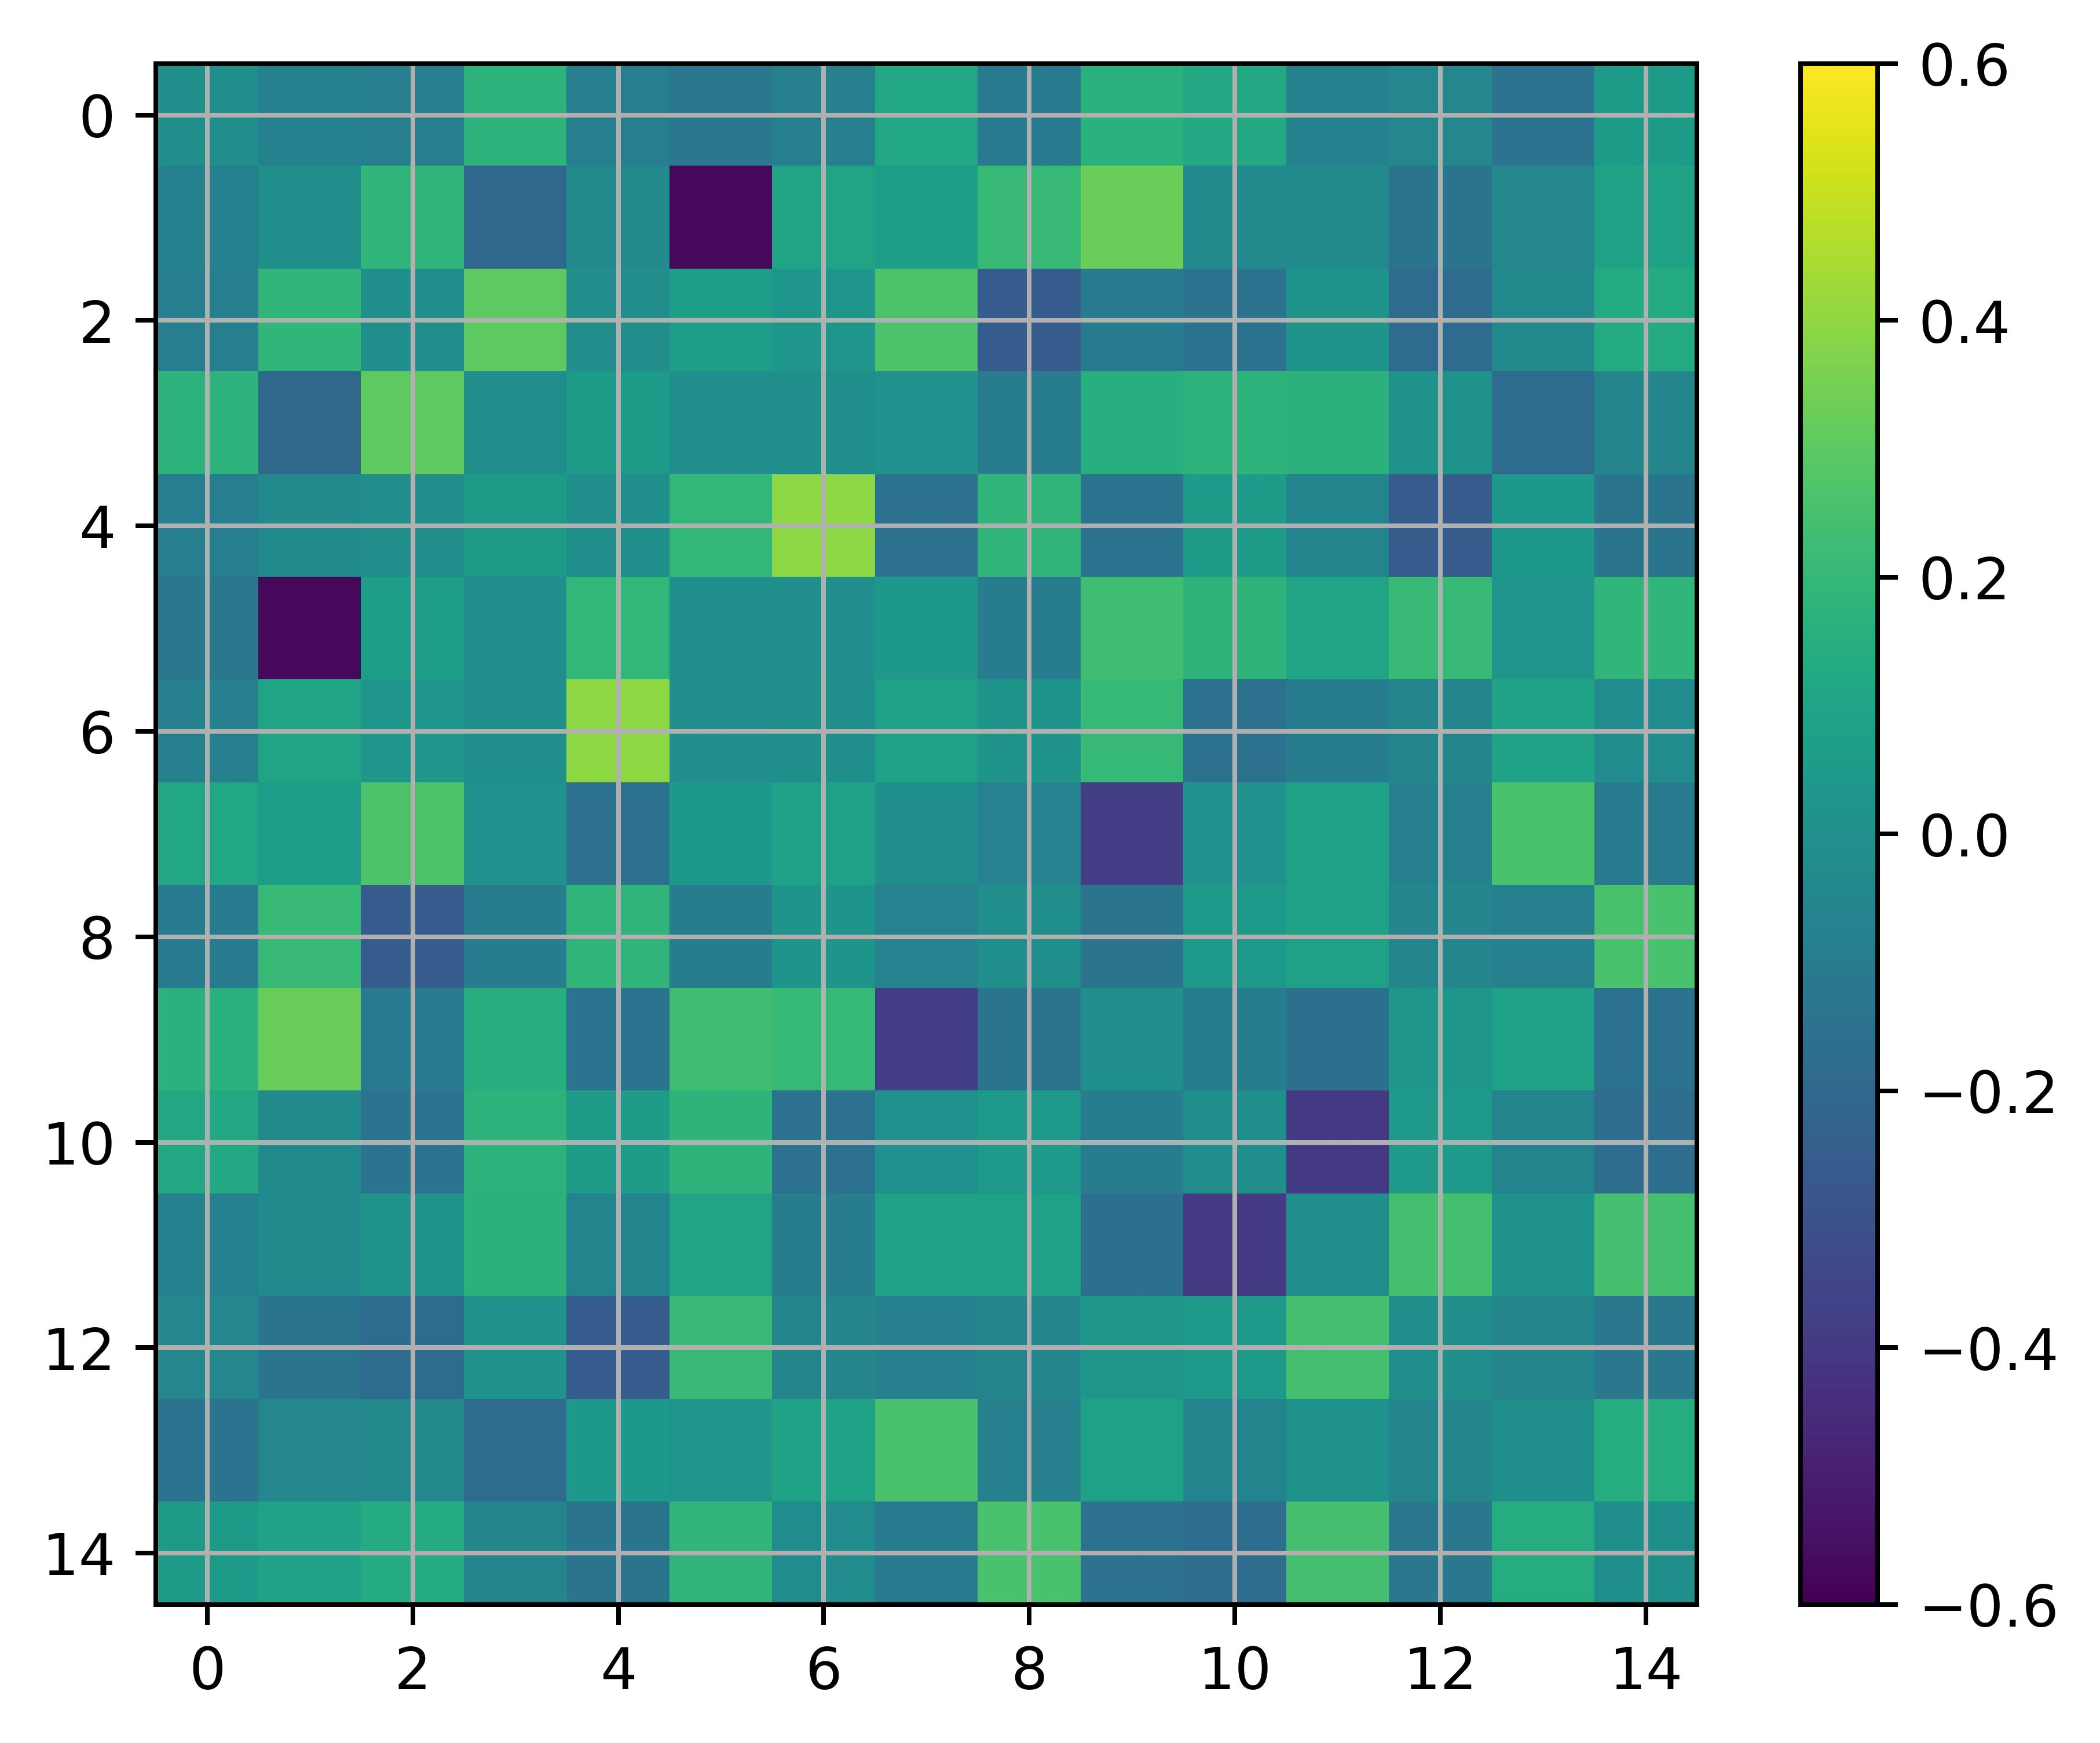
\includegraphics[width=1\textwidth]{../Analysis/DFC/size=480_step=180_rho=0.1/node=15_id=100206/0.jpg}
%                 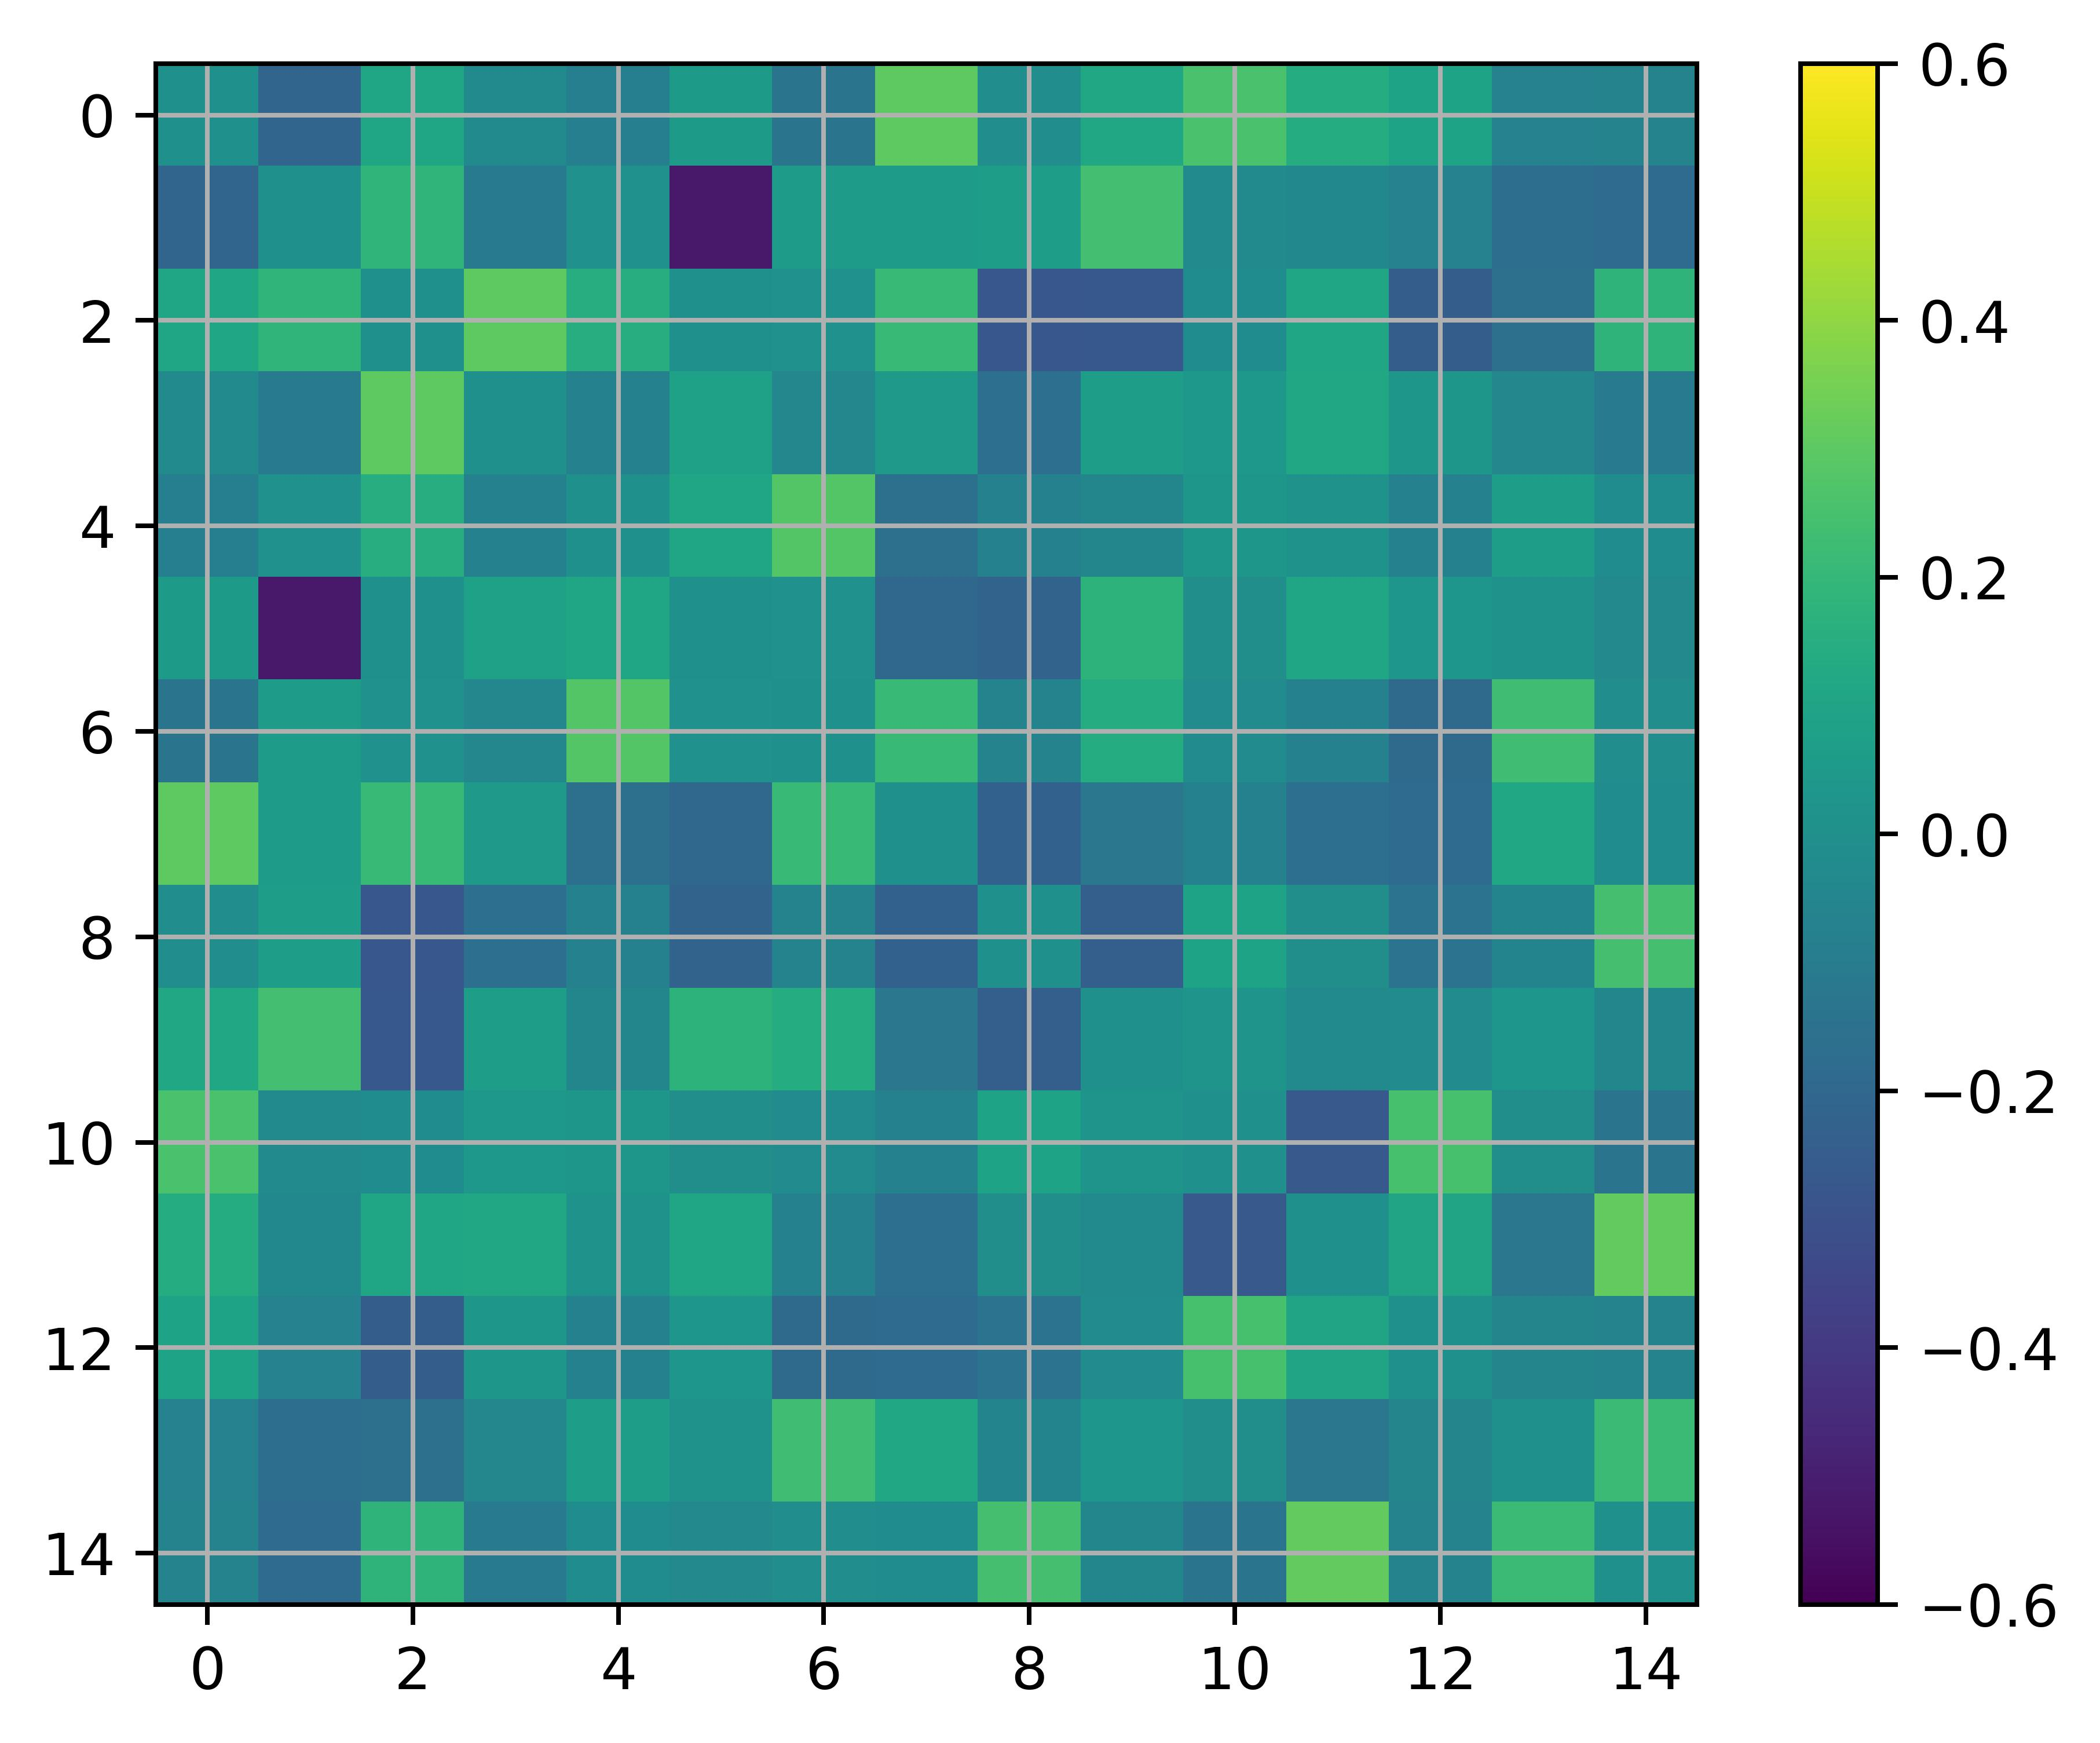
\includegraphics[width=1\textwidth]{../Analysis/DFC/size=480_step=180_rho=0.1/node=15_id=100206/10.jpg}
%                 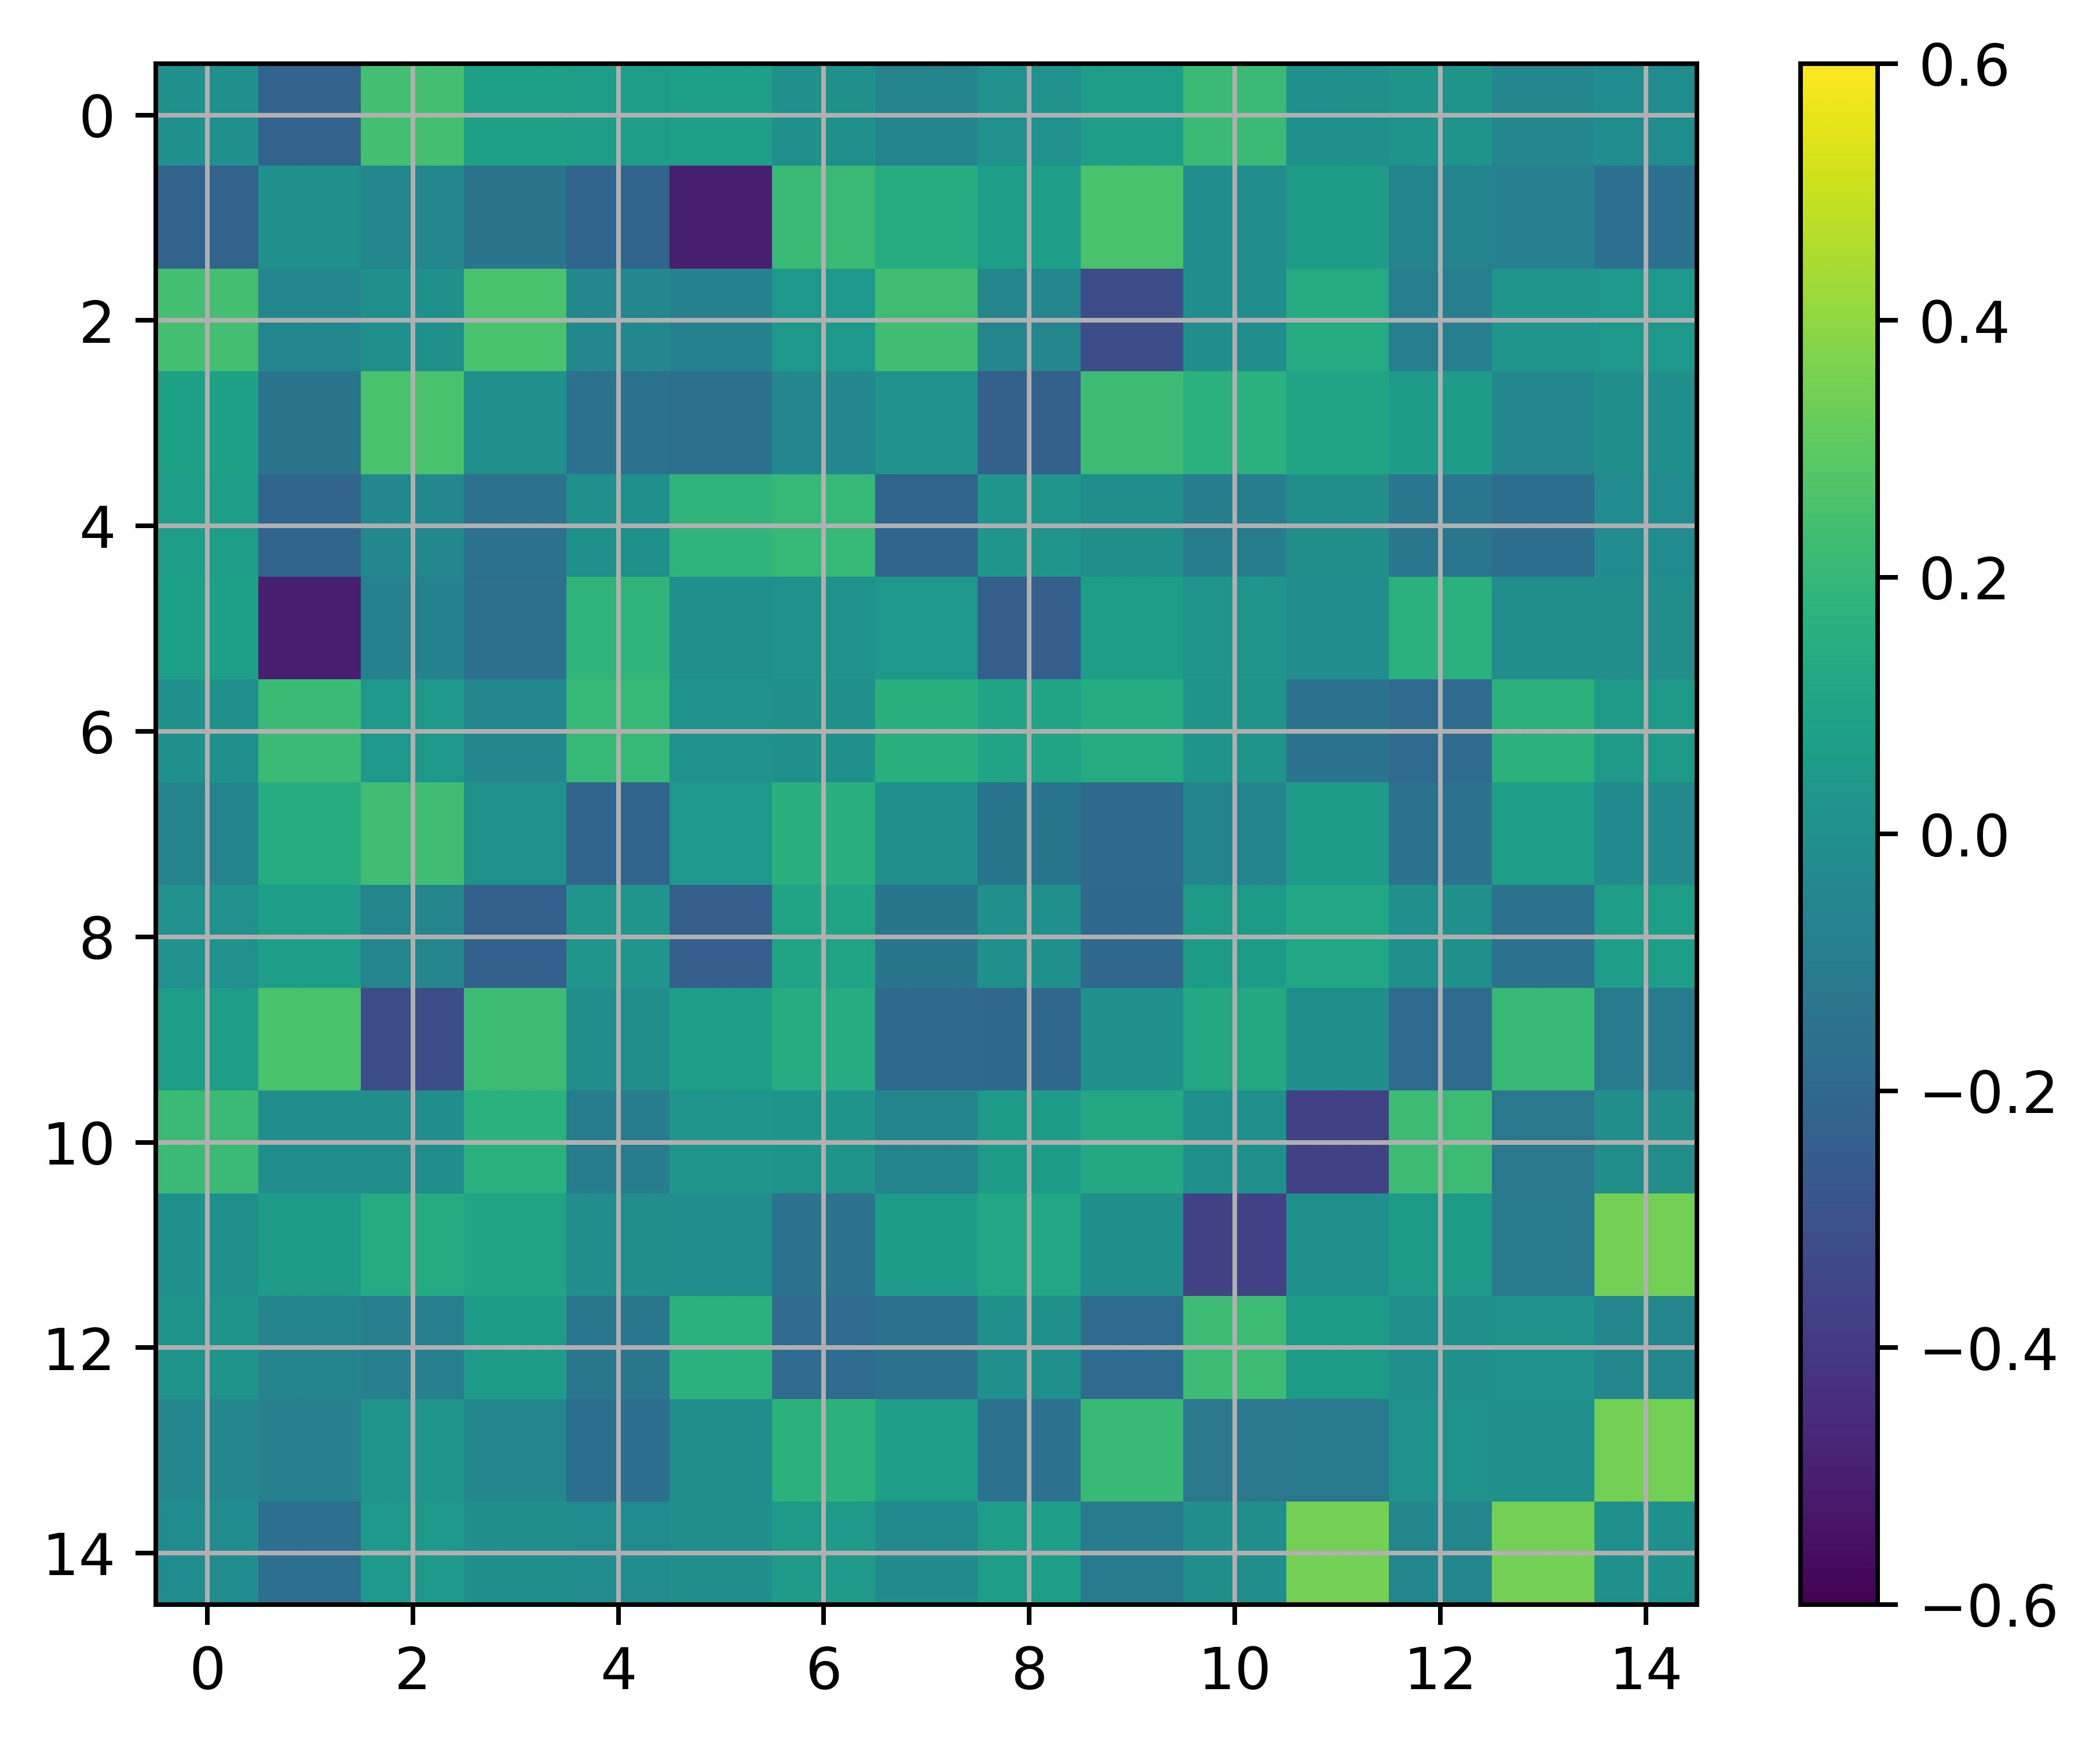
\includegraphics[width=1\textwidth]{../Analysis/DFC/size=480_step=180_rho=0.1/node=15_id=100206/20.jpg}
%             \end{minipage}
%         }
%         \subfloat[$N_{node} = 25$]{
%             \begin{minipage}[b]{0.2\textwidth}
%                 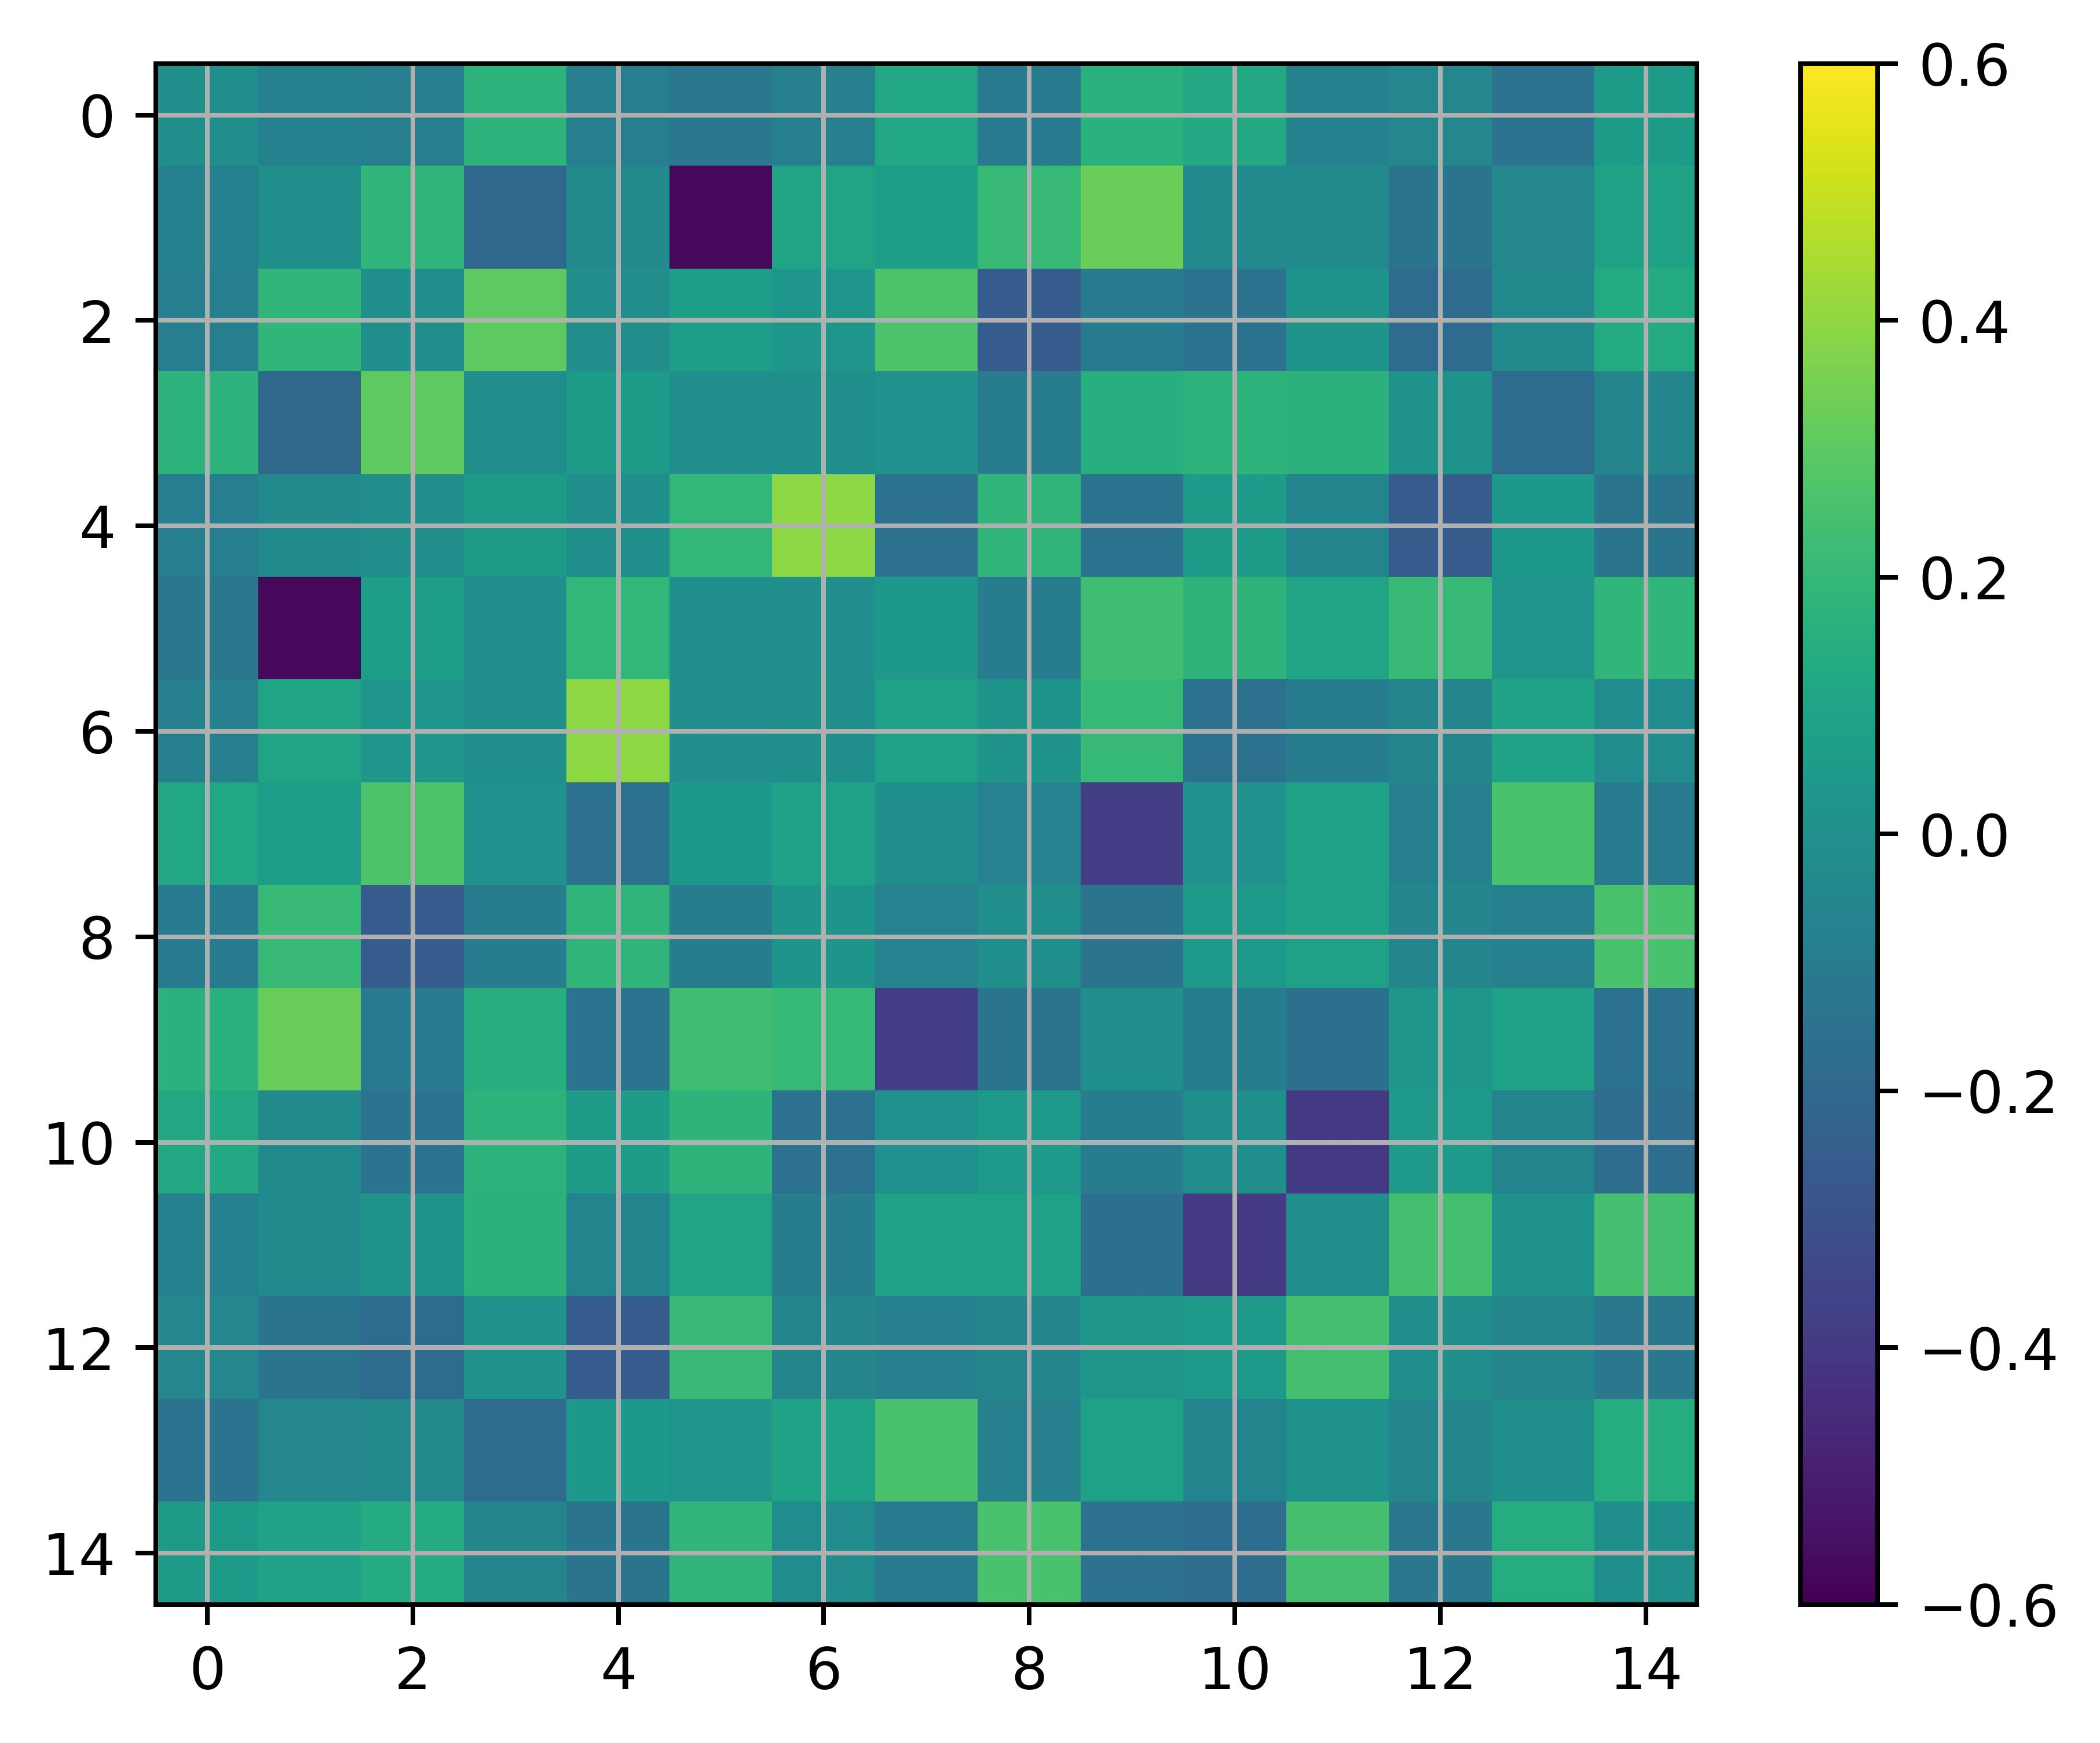
\includegraphics[width=1\textwidth]{../Analysis/DFC/size=480_step=180_rho=0.1/node=15_id=100206/0.jpg}
%                 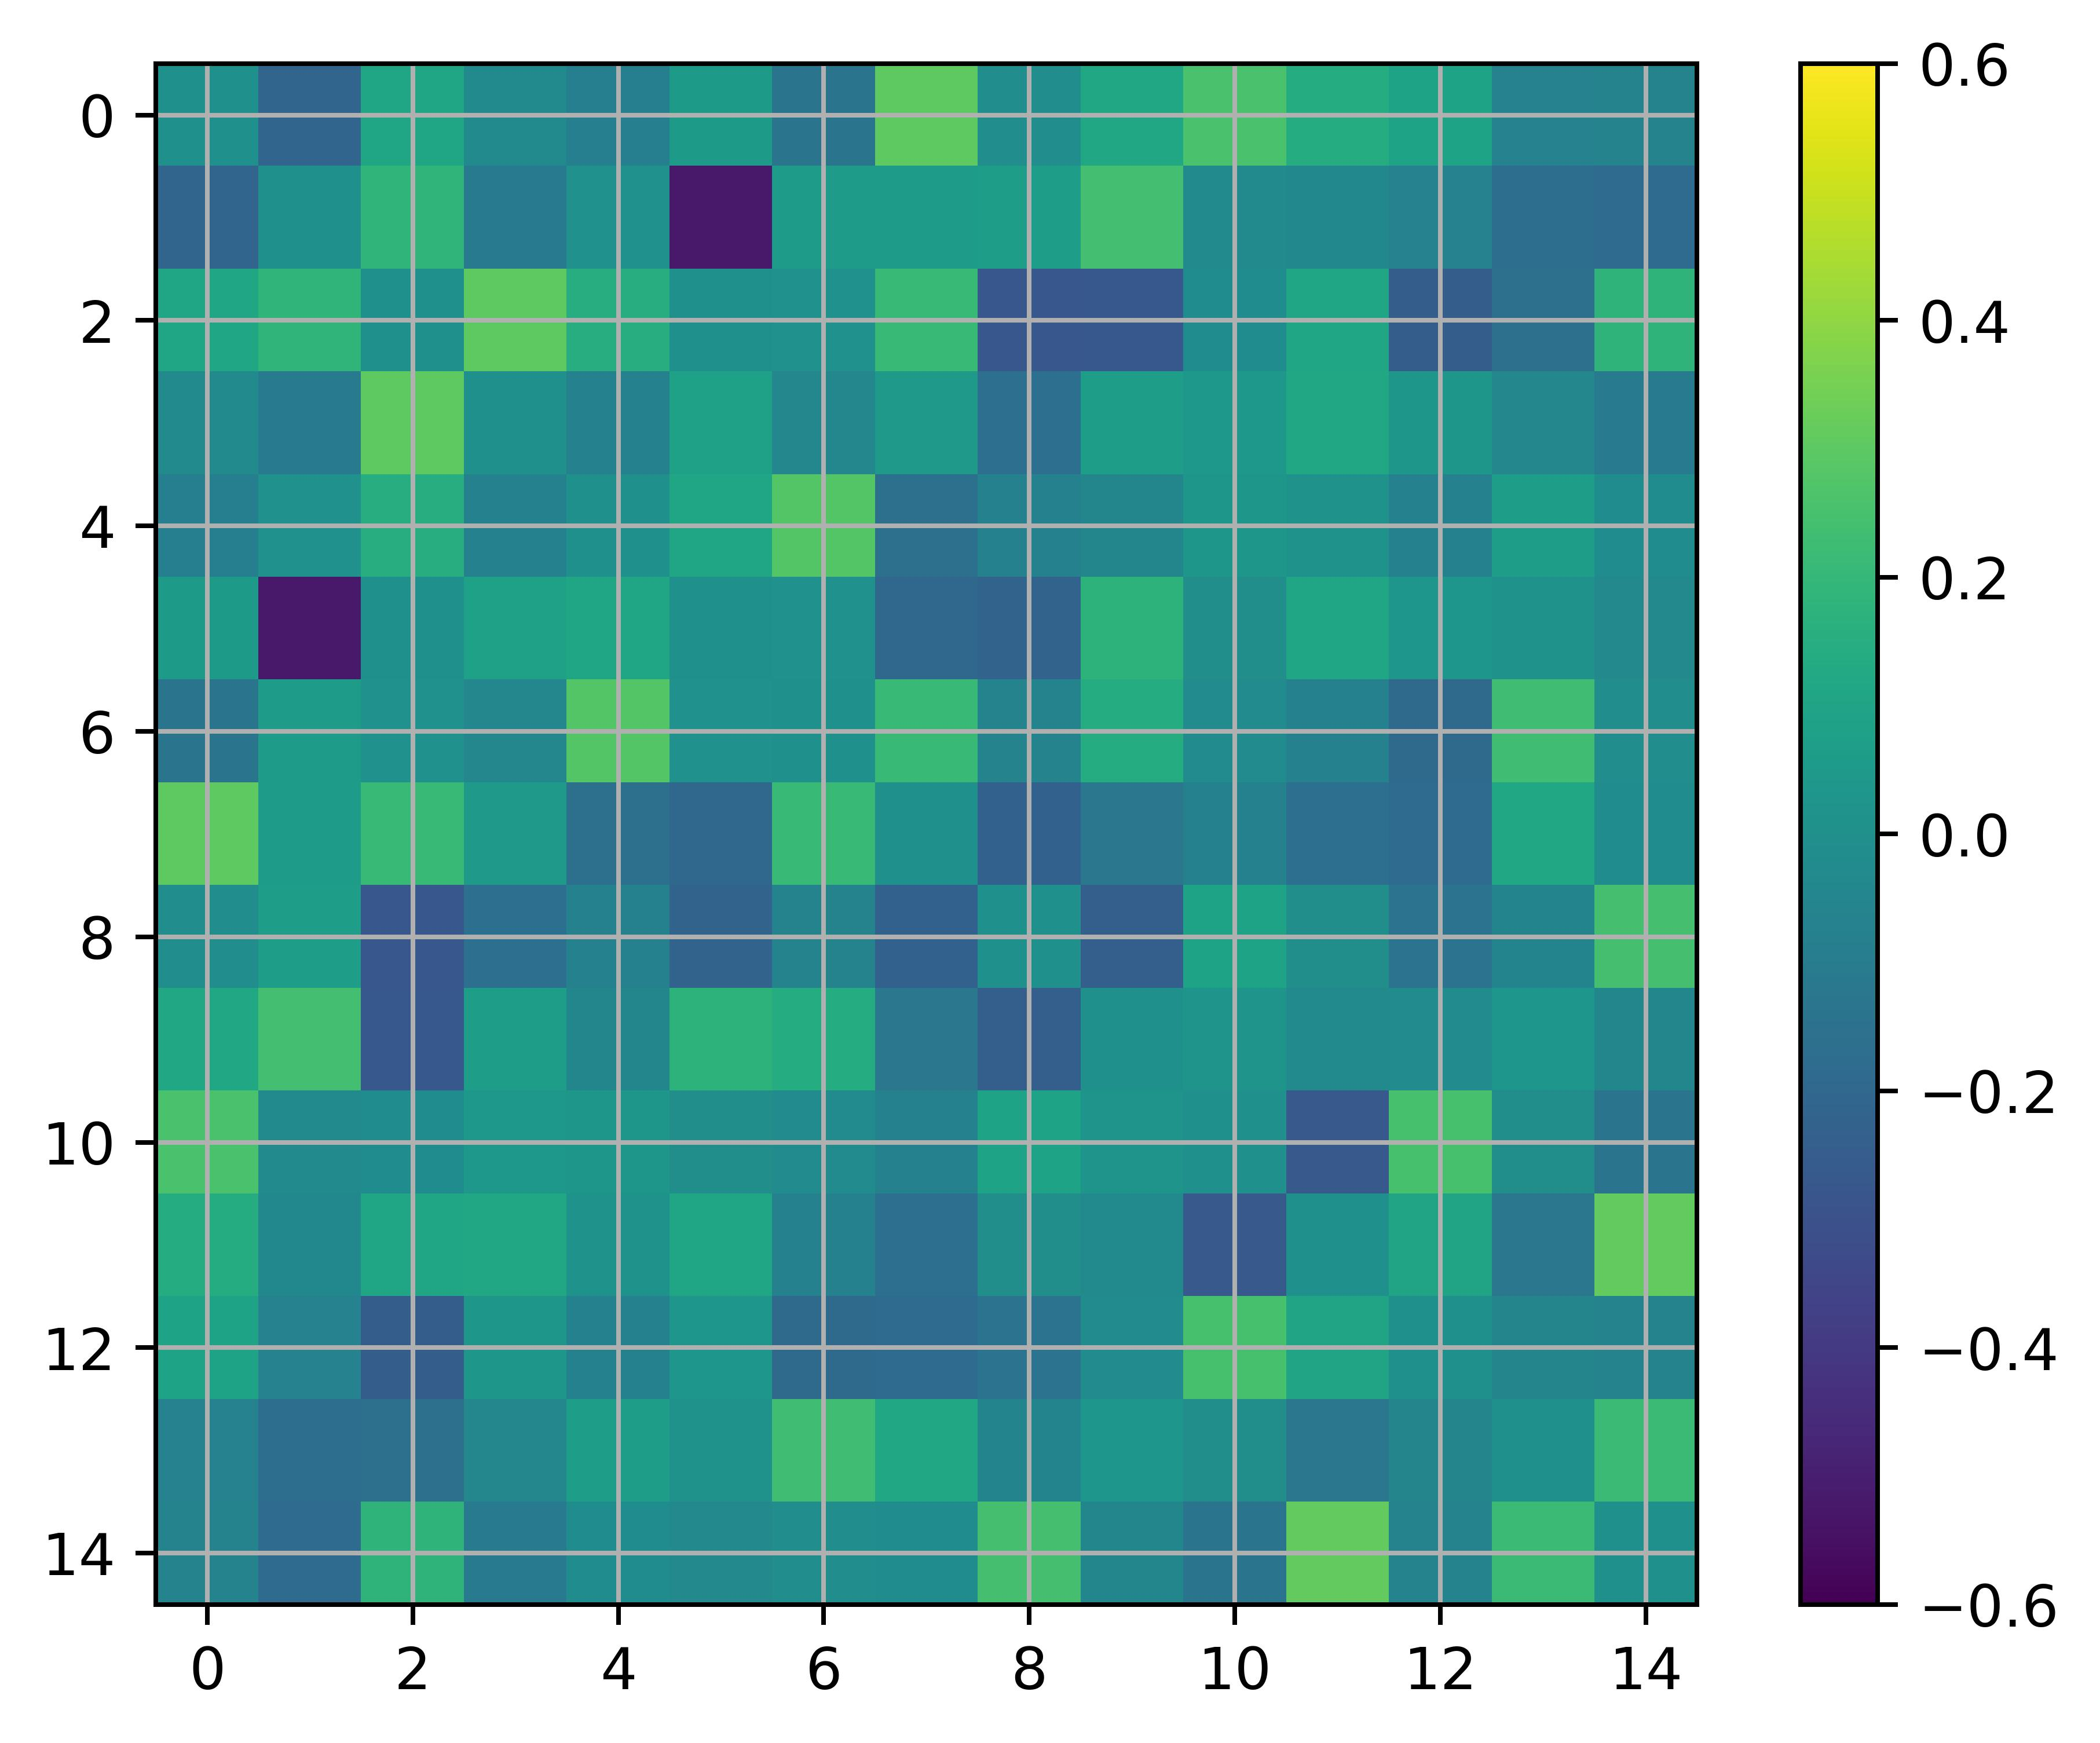
\includegraphics[width=1\textwidth]{../Analysis/DFC/size=480_step=180_rho=0.1/node=15_id=100206/10.jpg}
%                 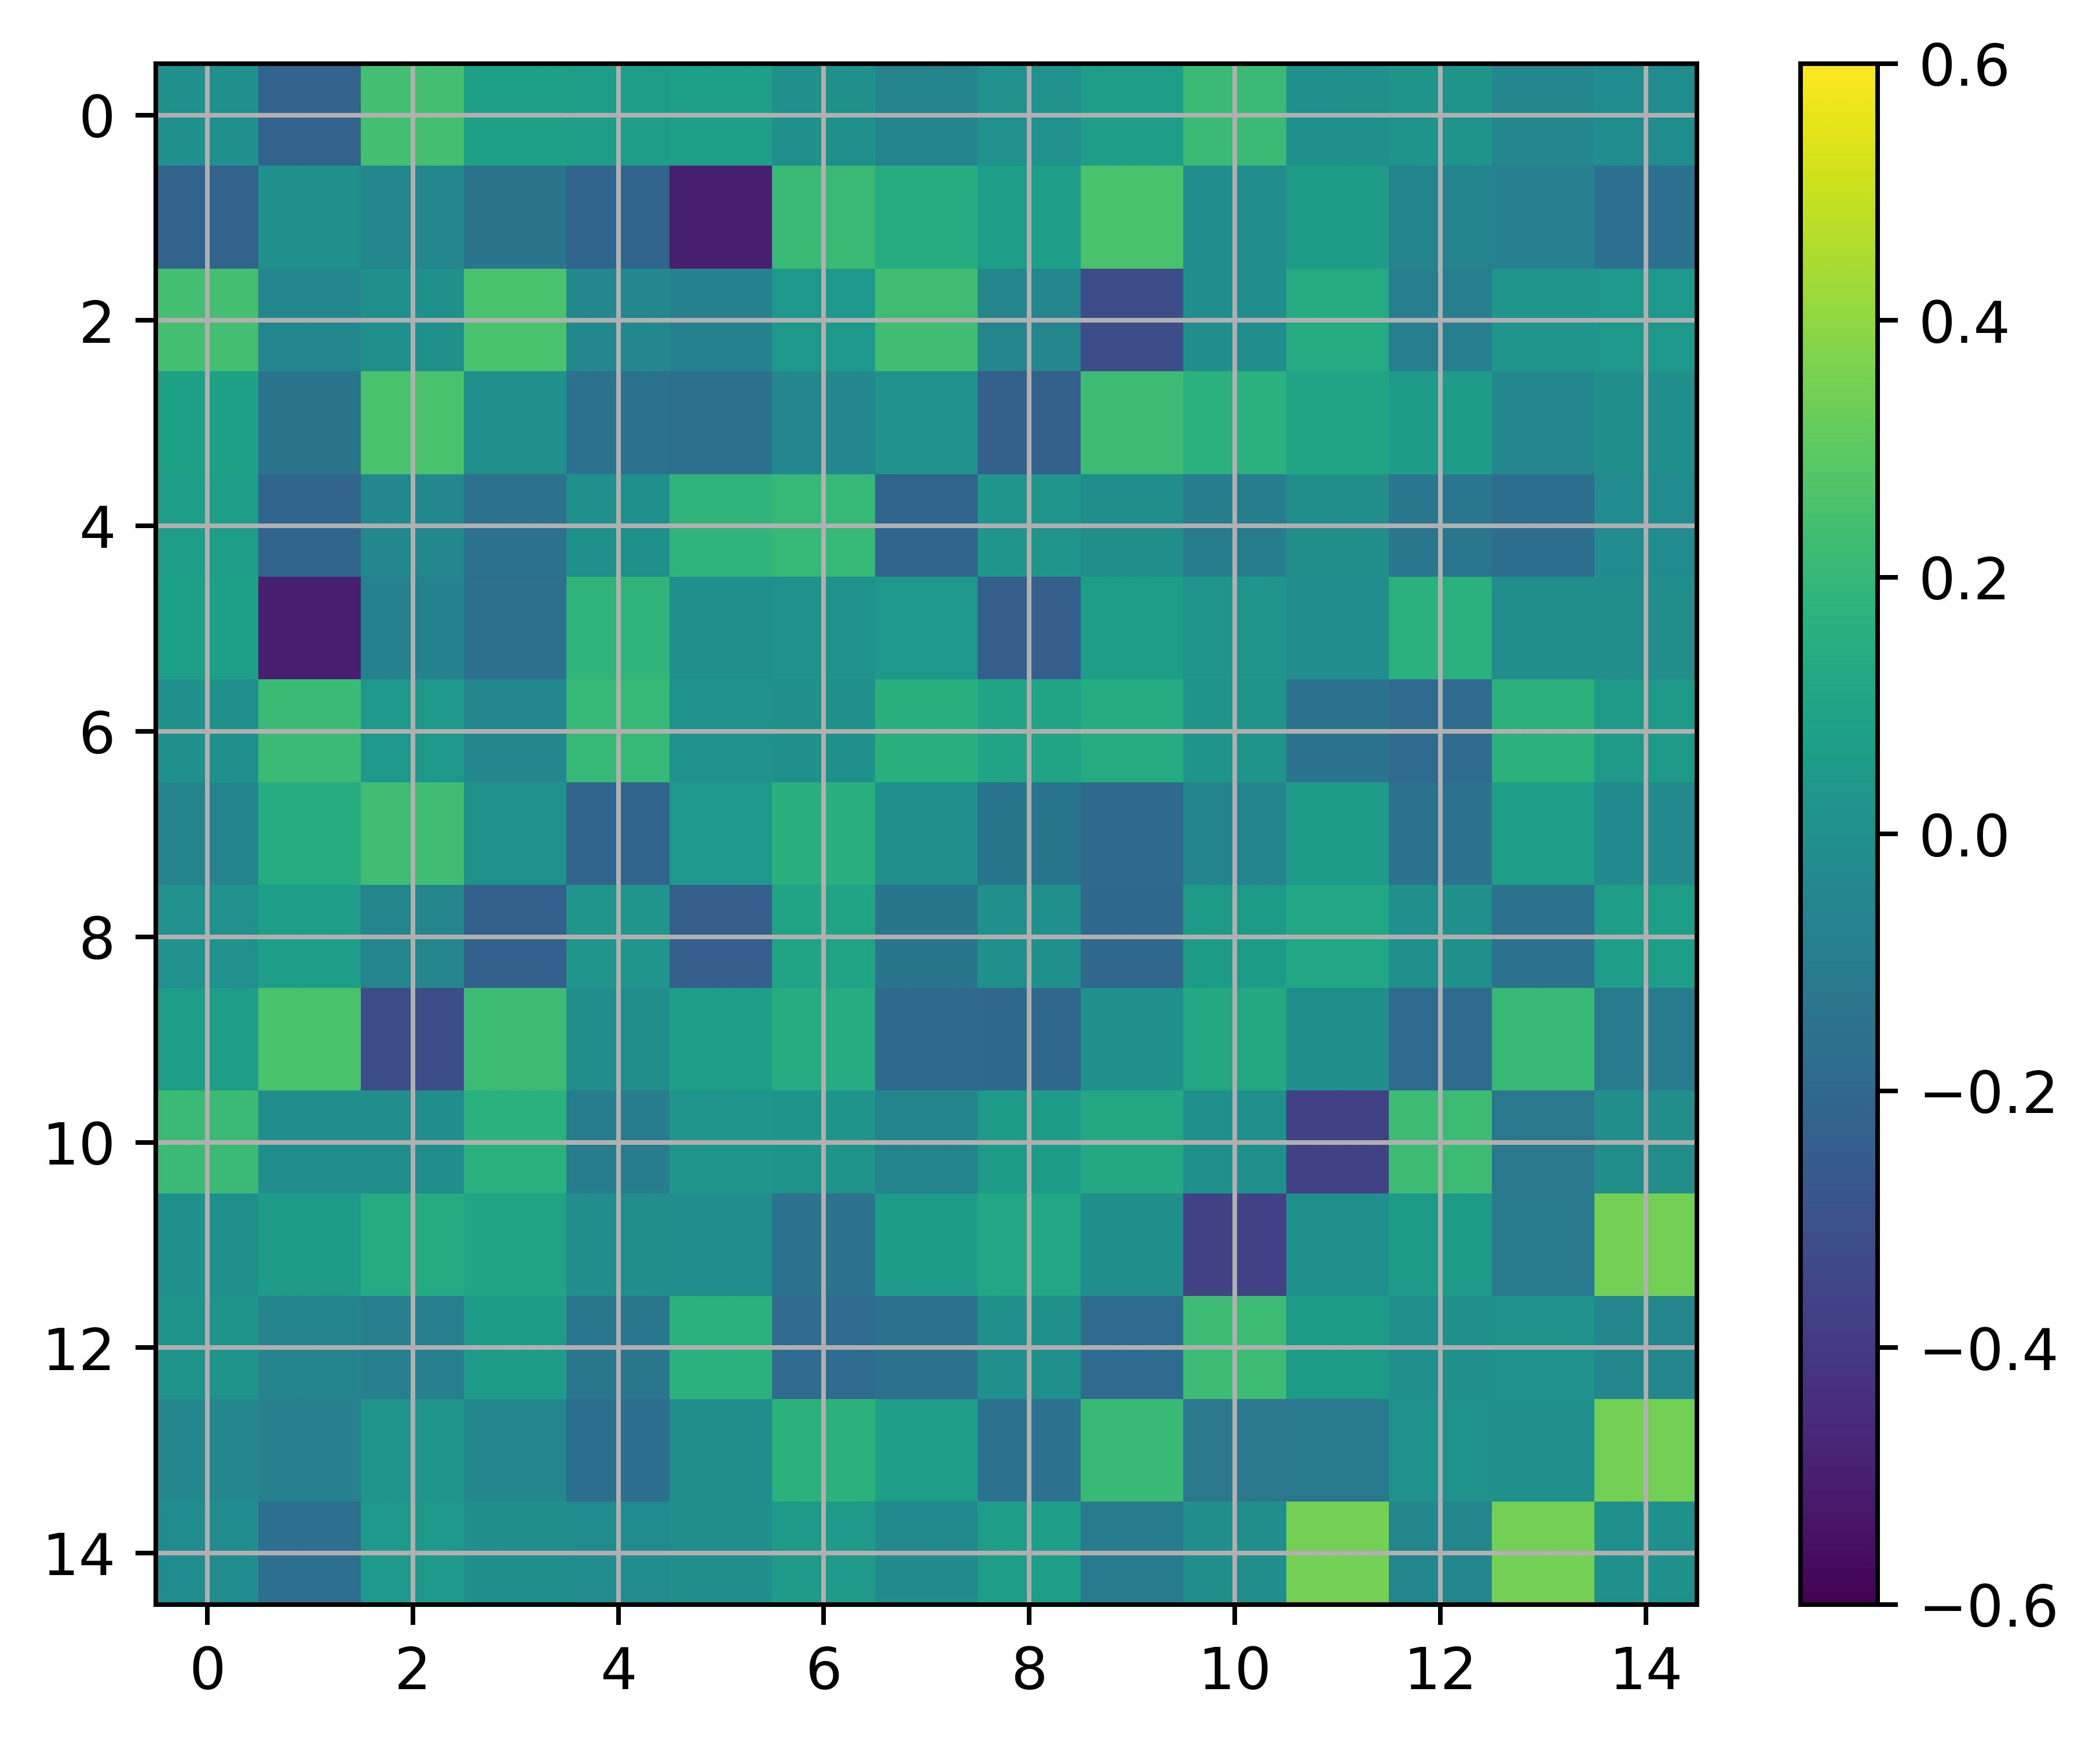
\includegraphics[width=1\textwidth]{../Analysis/DFC/size=480_step=180_rho=0.1/node=15_id=100206/20.jpg}
%             \end{minipage}
%         }
%         \subfloat[$N_{node} = 50$]{
%             \begin{minipage}[b]{0.2\textwidth}
%                 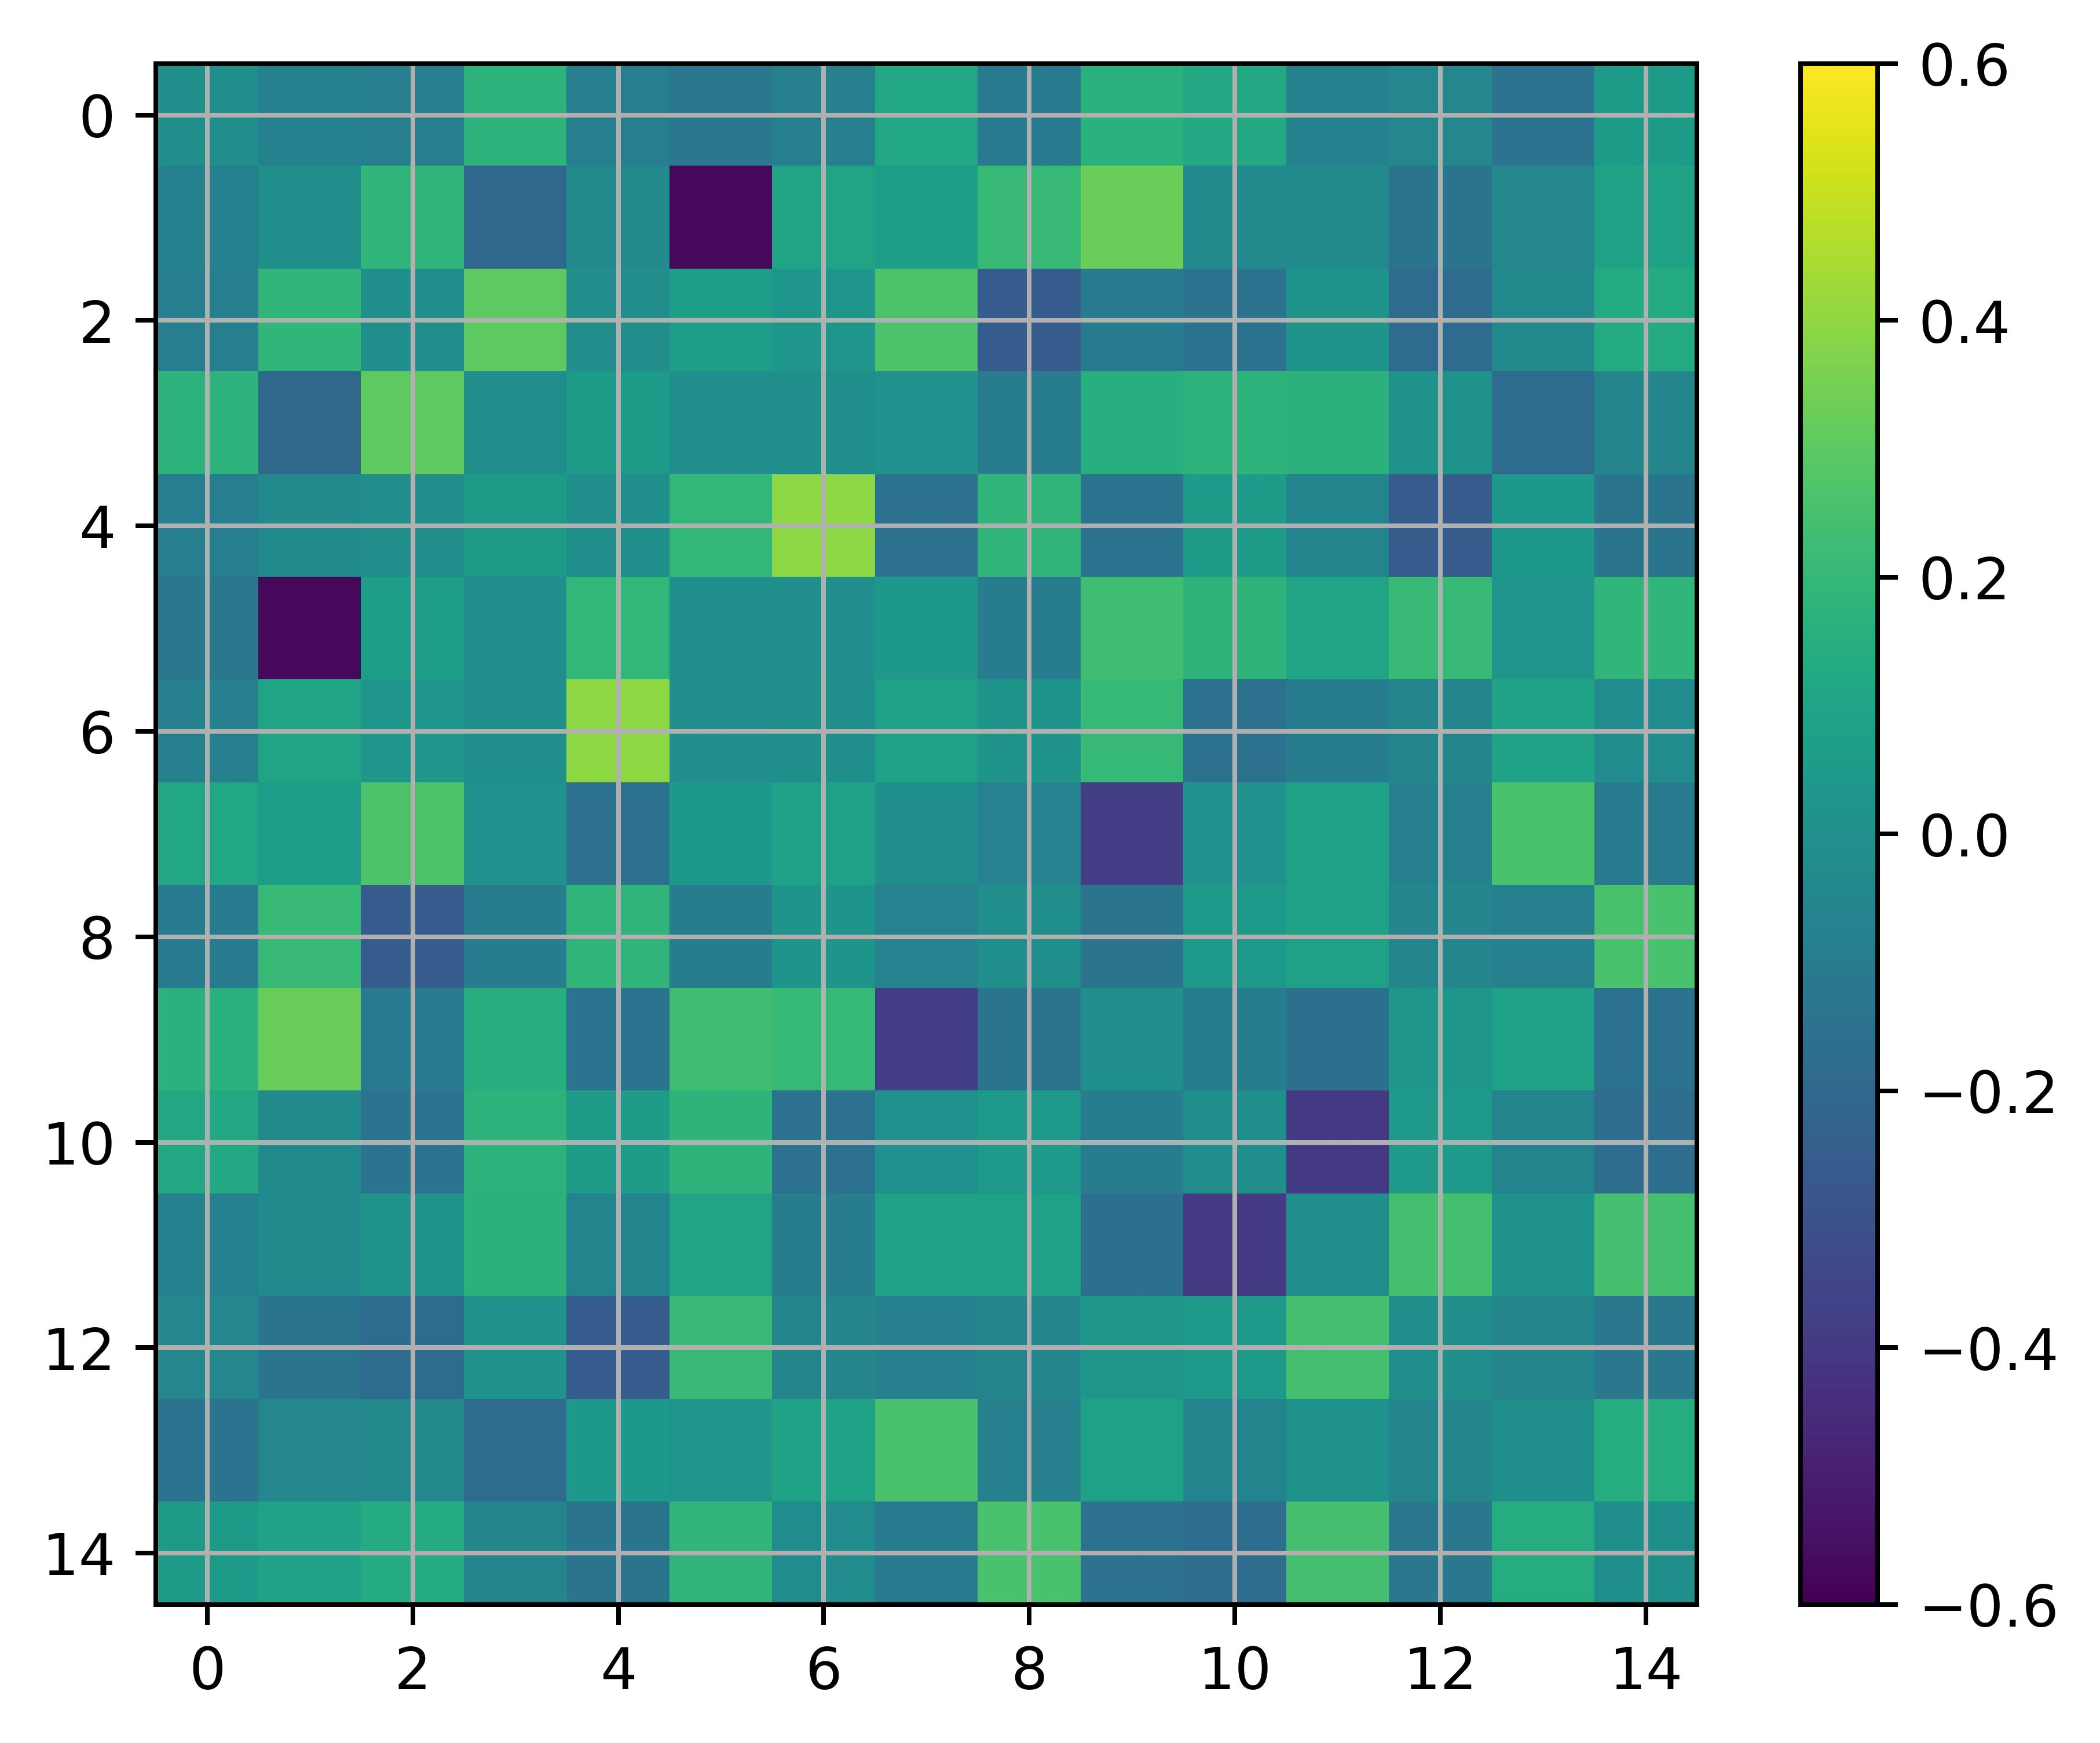
\includegraphics[width=1\textwidth]{../Analysis/DFC/size=480_step=180_rho=0.1/node=15_id=100206/0.jpg}
%                 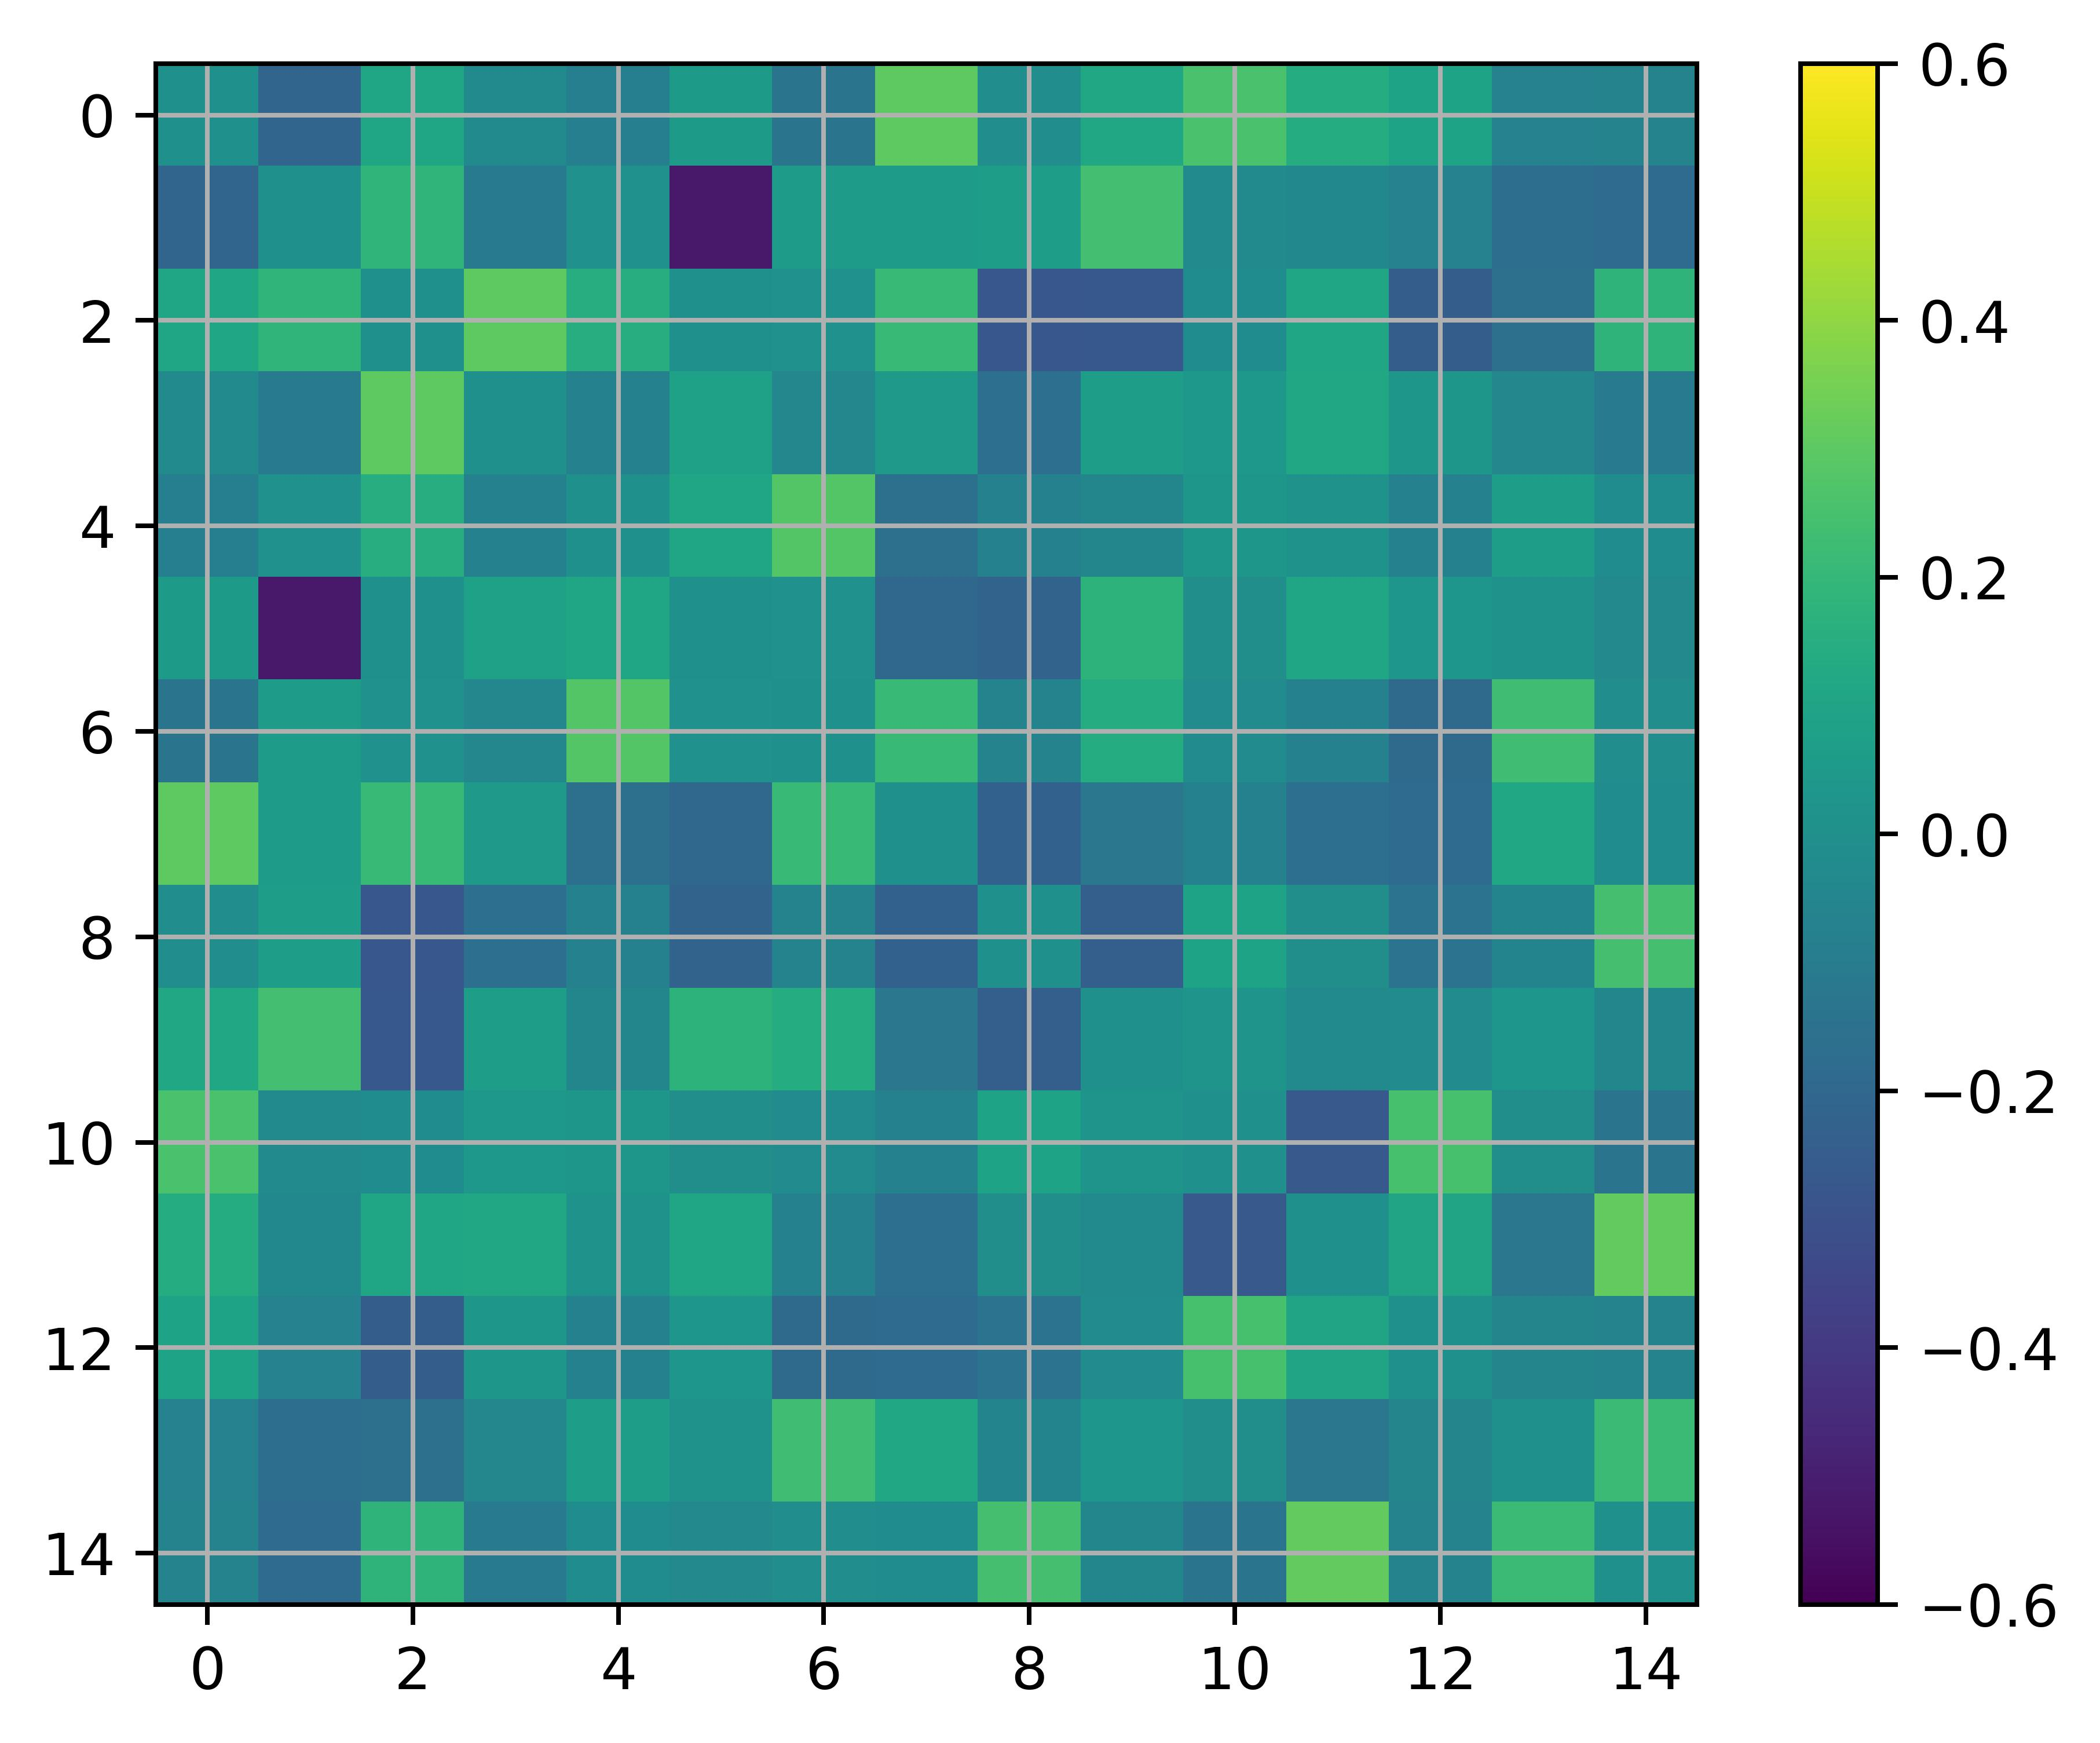
\includegraphics[width=1\textwidth]{../Analysis/DFC/size=480_step=180_rho=0.1/node=15_id=100206/10.jpg}
%                 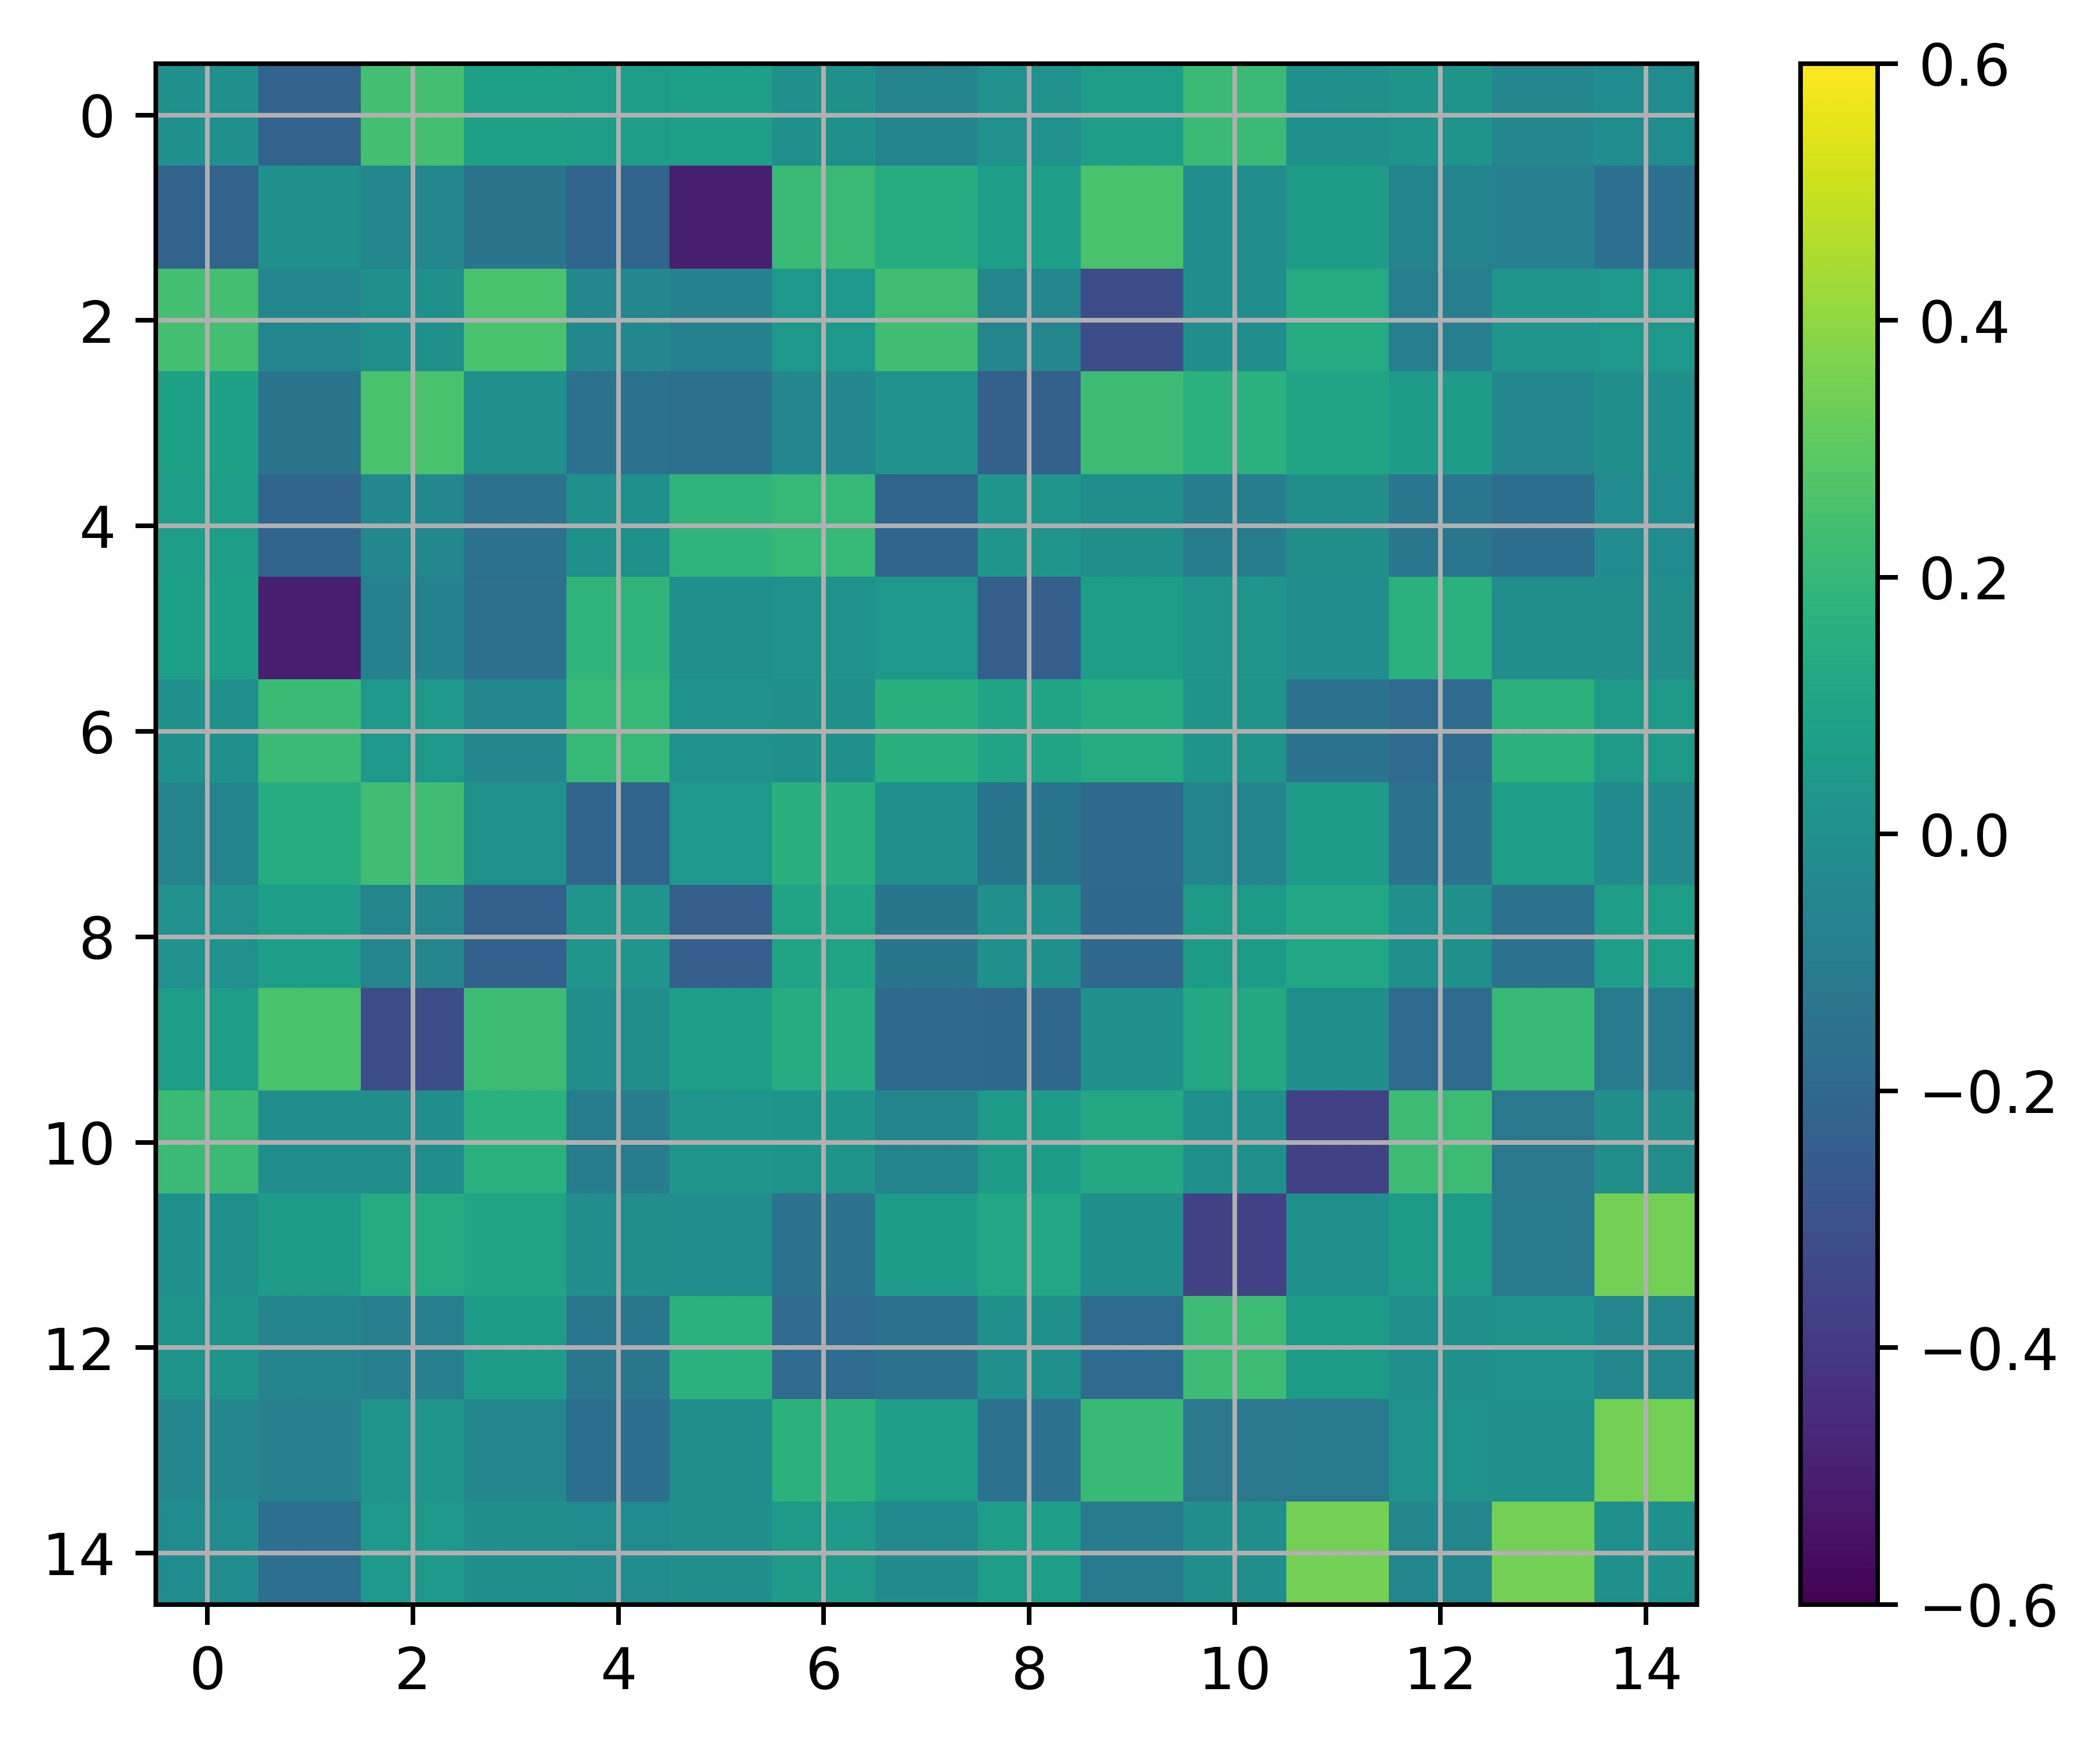
\includegraphics[width=1\textwidth]{../Analysis/DFC/size=480_step=180_rho=0.1/node=15_id=100206/20.jpg}
%             \end{minipage}
%         }
%         % \caption{LDA for static connectivity with $N_{node} = 15$.}
%         % \label{LDA-example-1}
%     \end{figure}

% \end{frame}

\begin{frame}{Preprocessing - Examples}

    \begin{figure}[H]
        \centering
        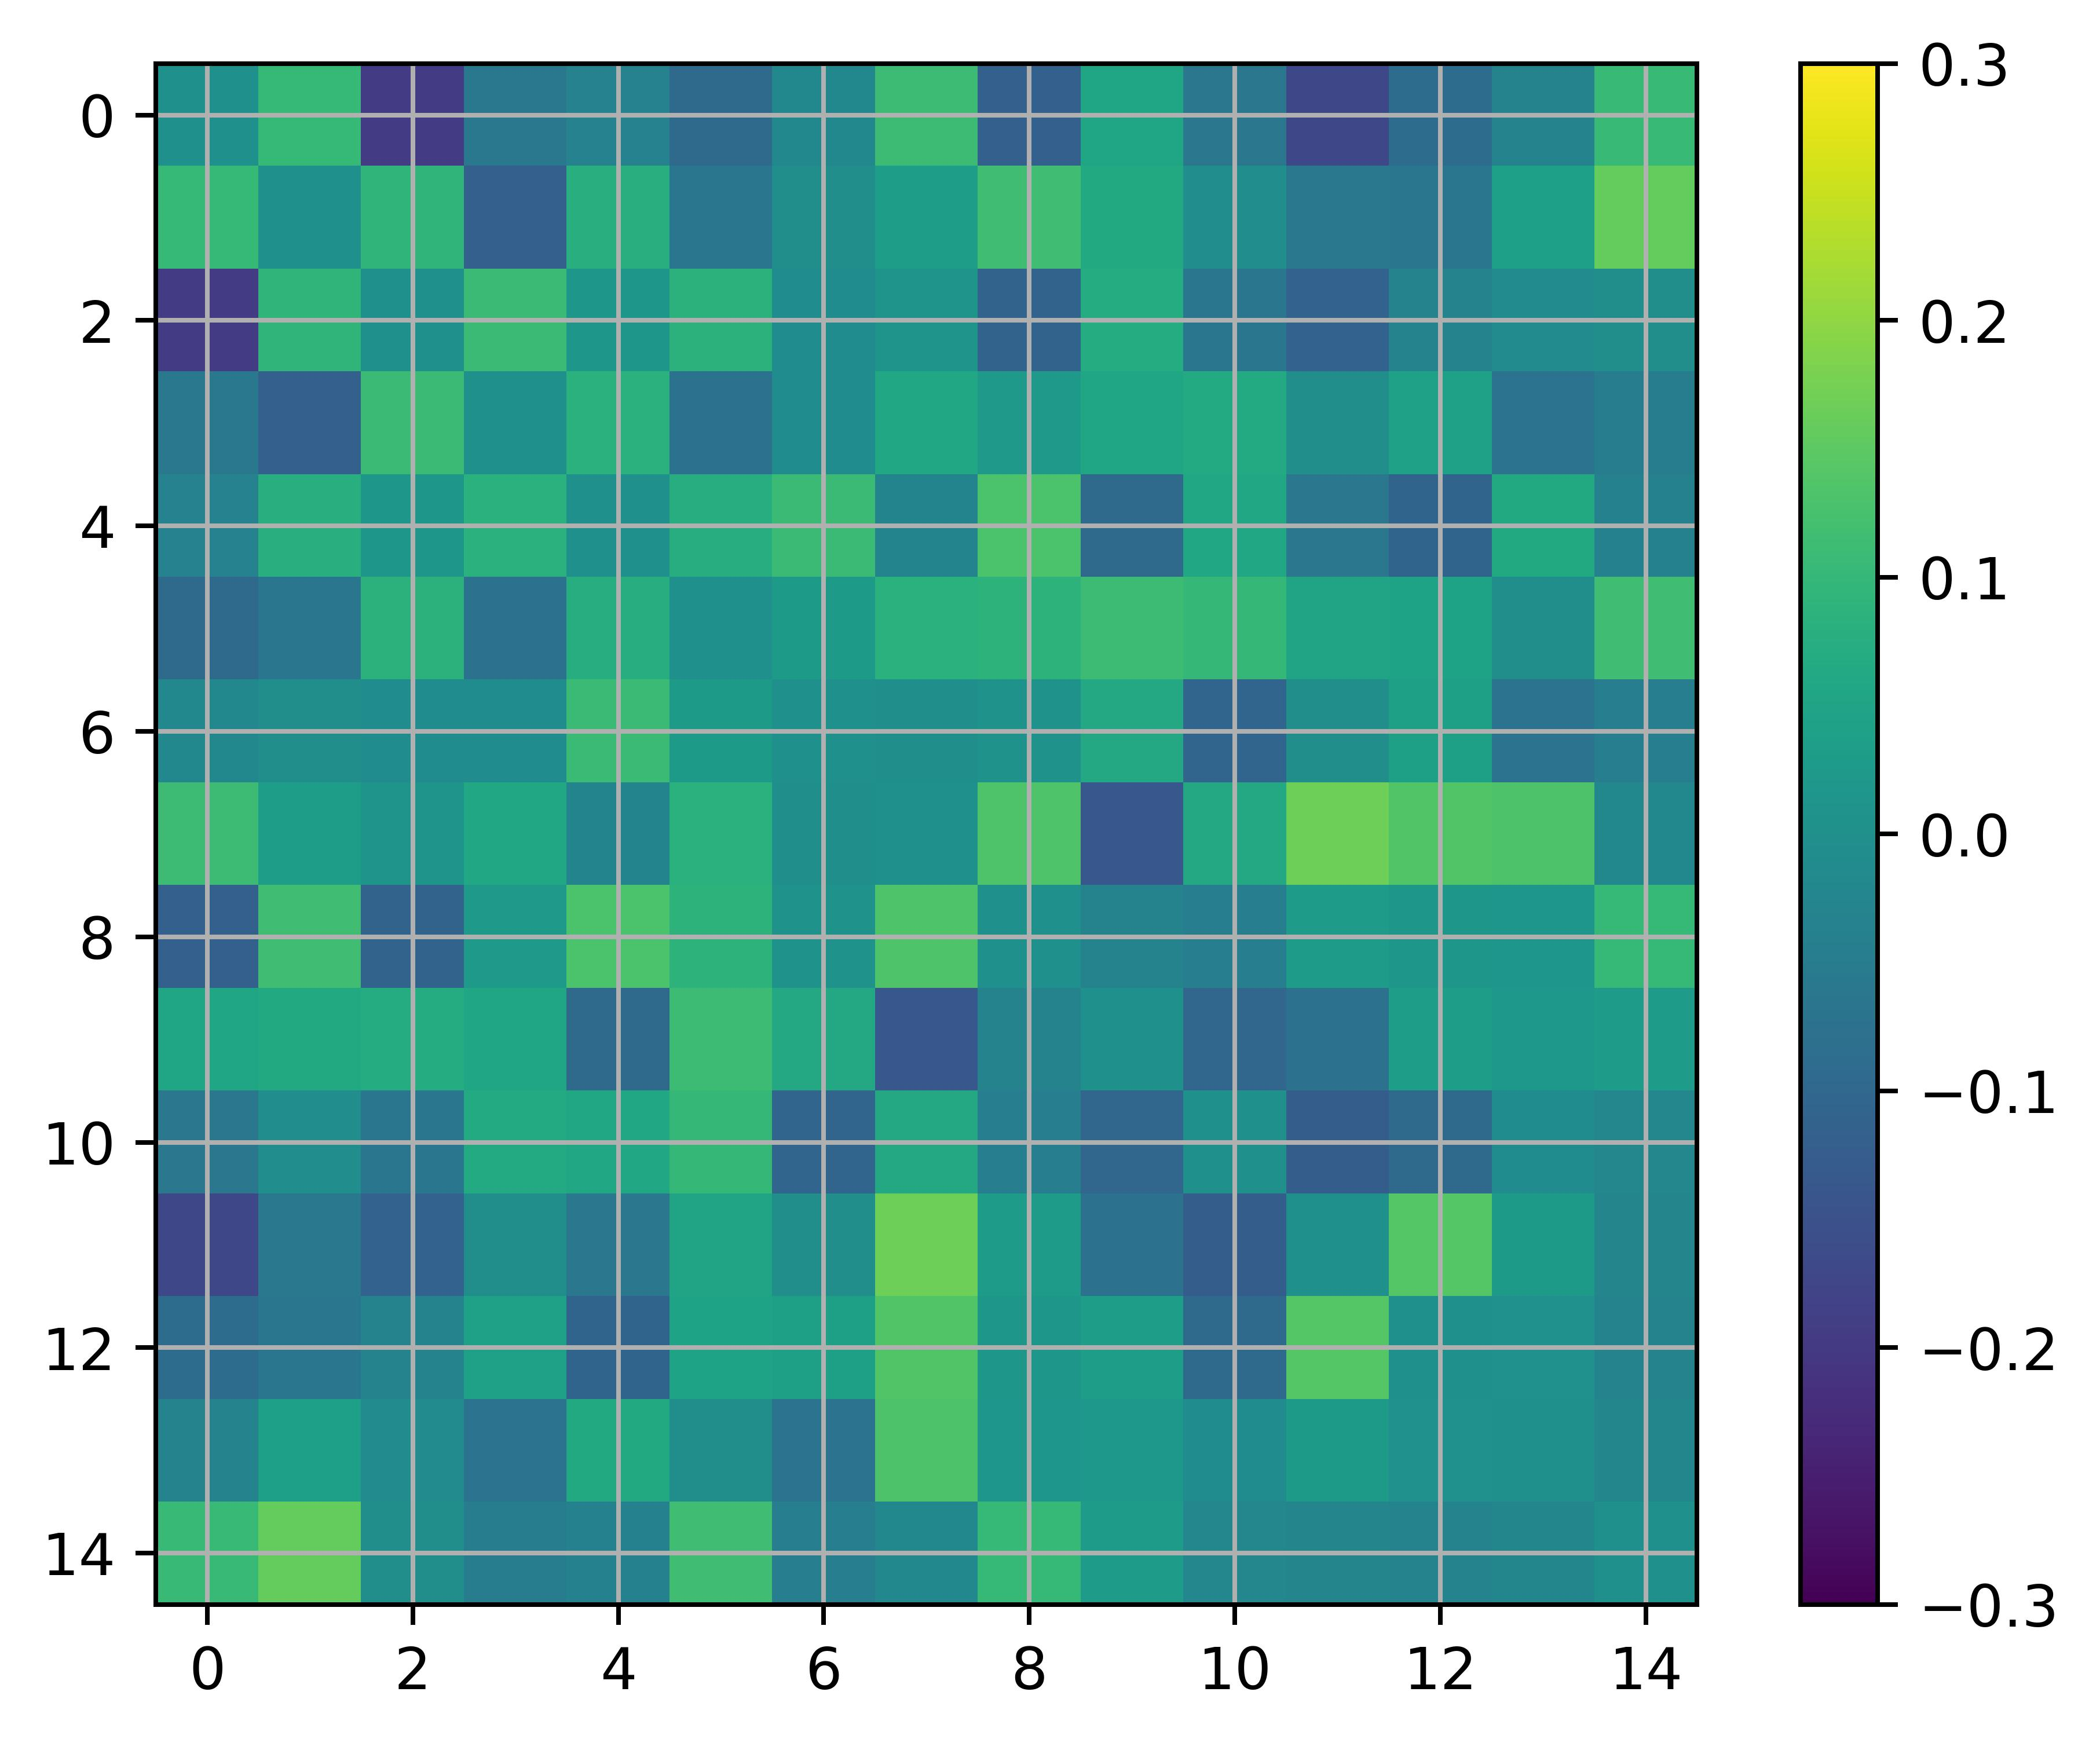
\includegraphics[width=0.2\textwidth]{../Analysis/DFC/size=480_step=180_rho=0.1/node=15_id=100206/c_0.jpg}
        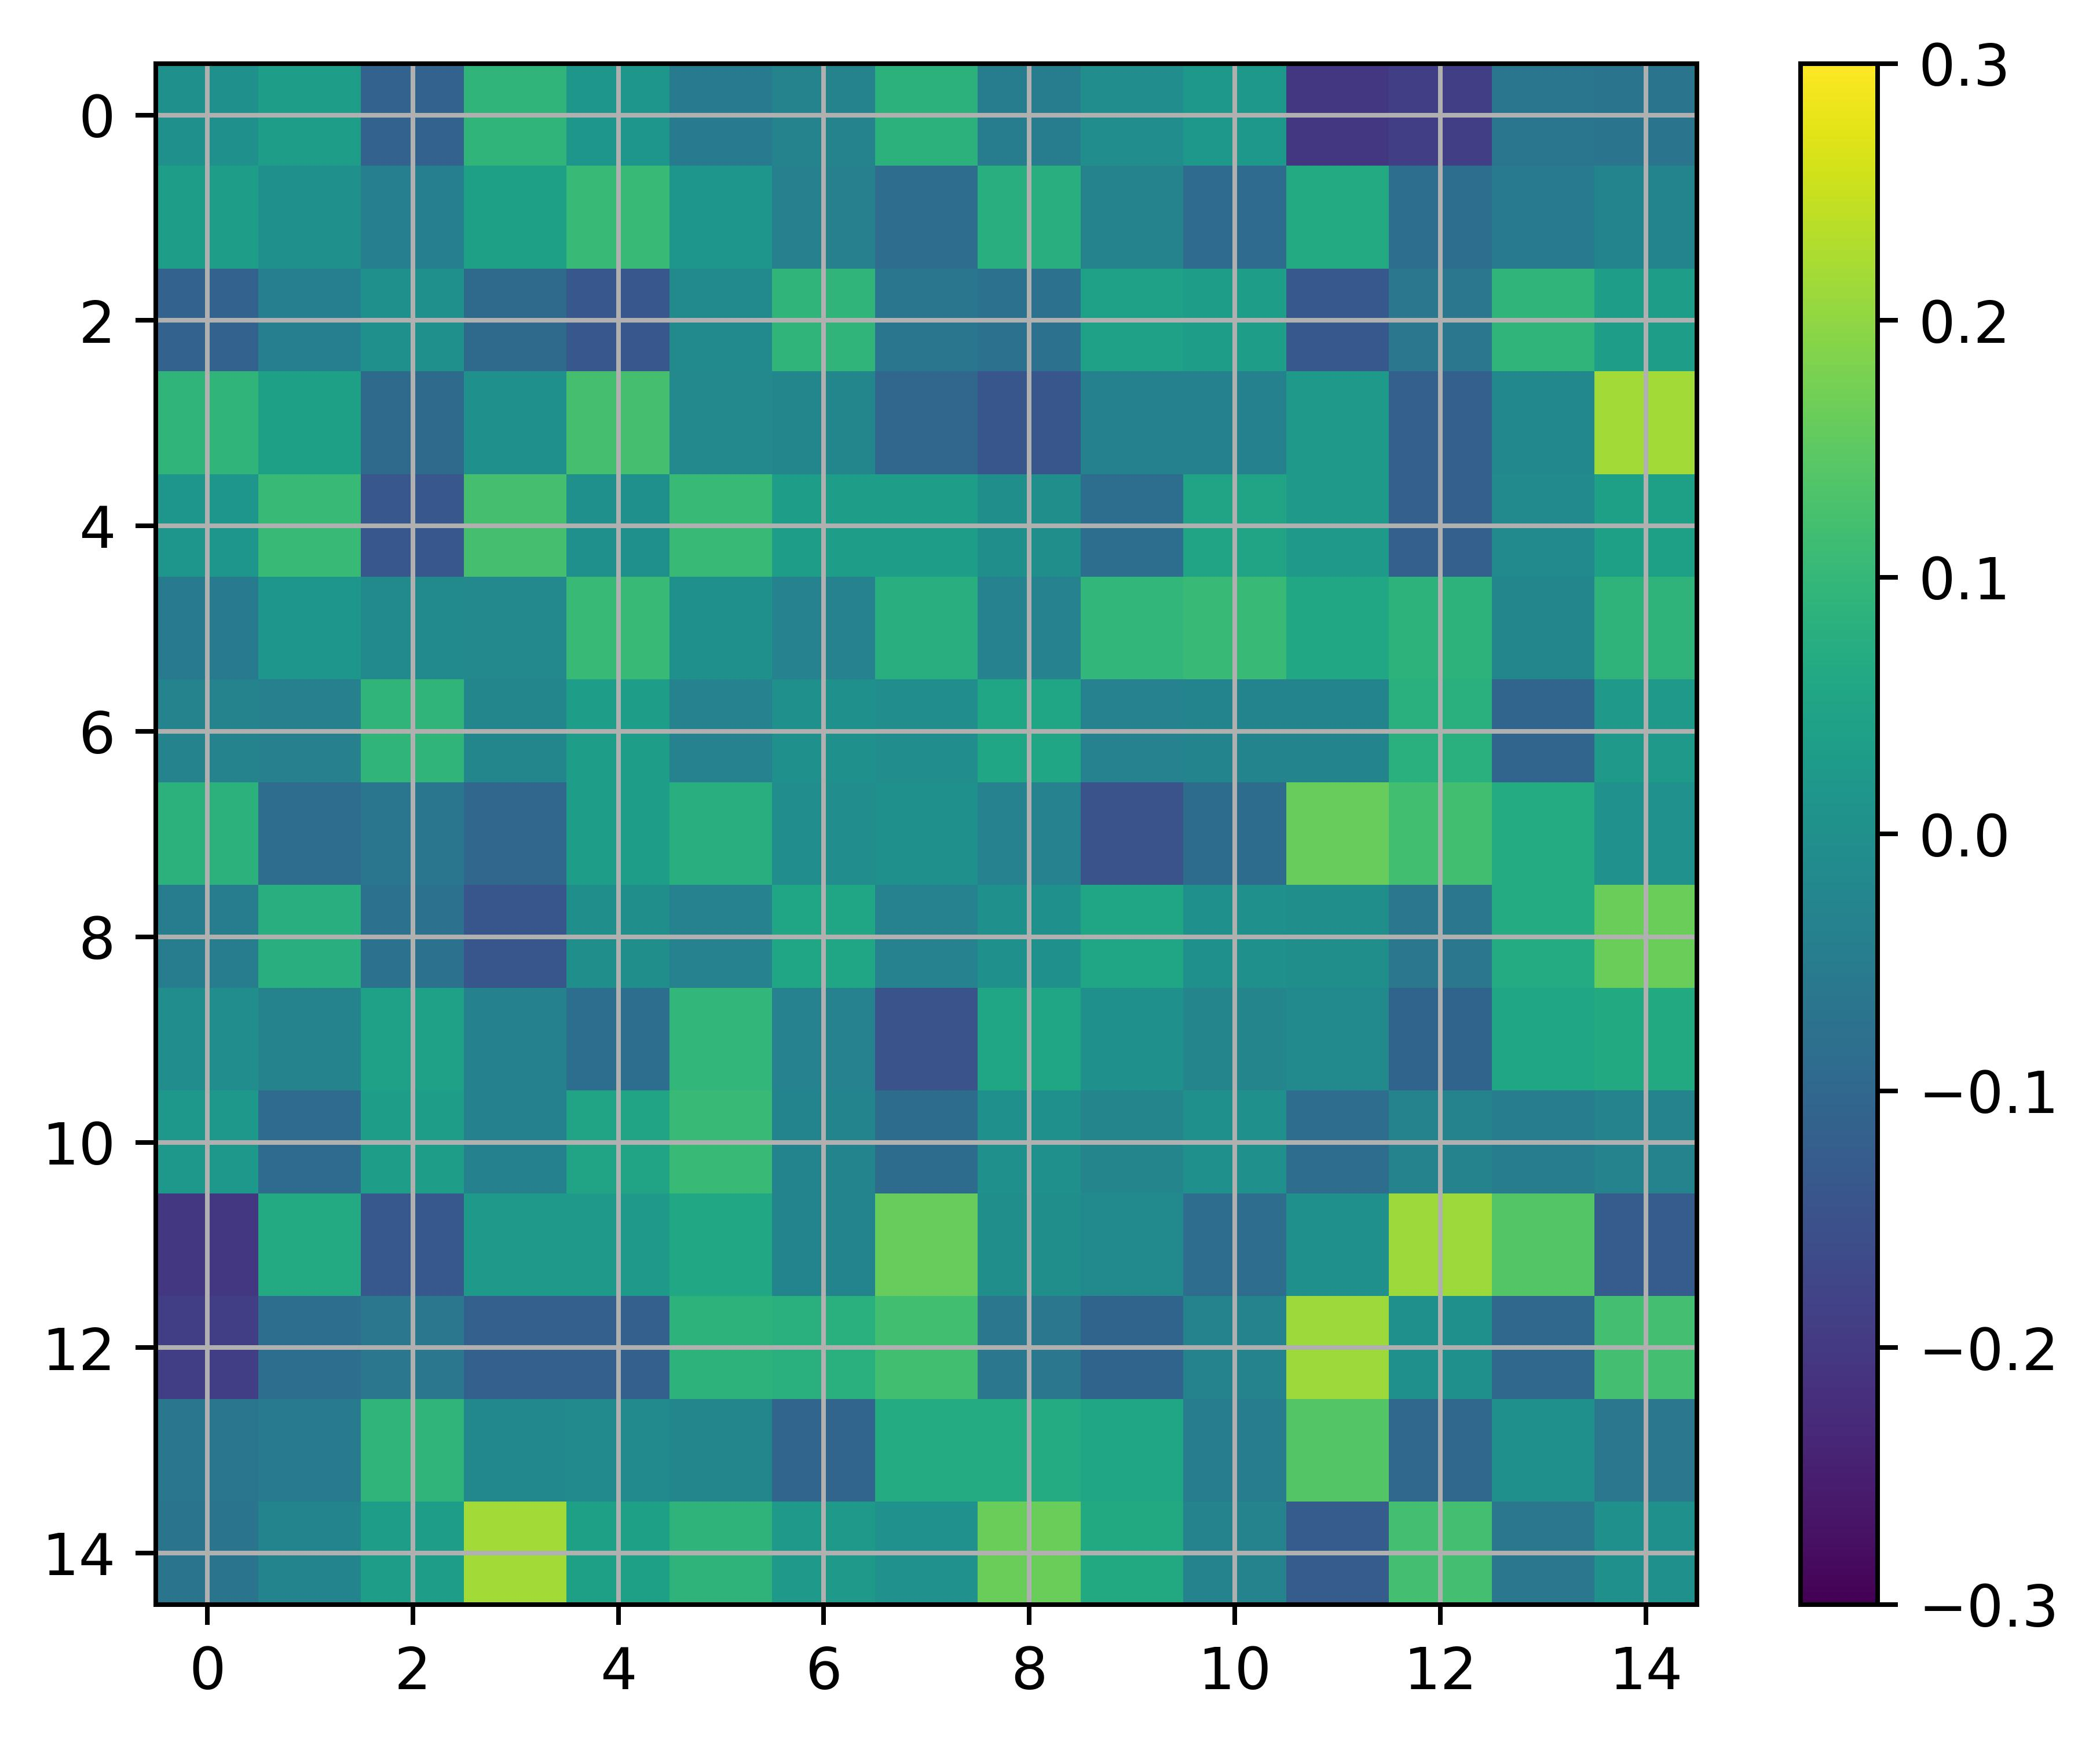
\includegraphics[width=0.2\textwidth]{../Analysis/DFC/size=480_step=180_rho=0.1/node=15_id=100206/c_2.jpg}
        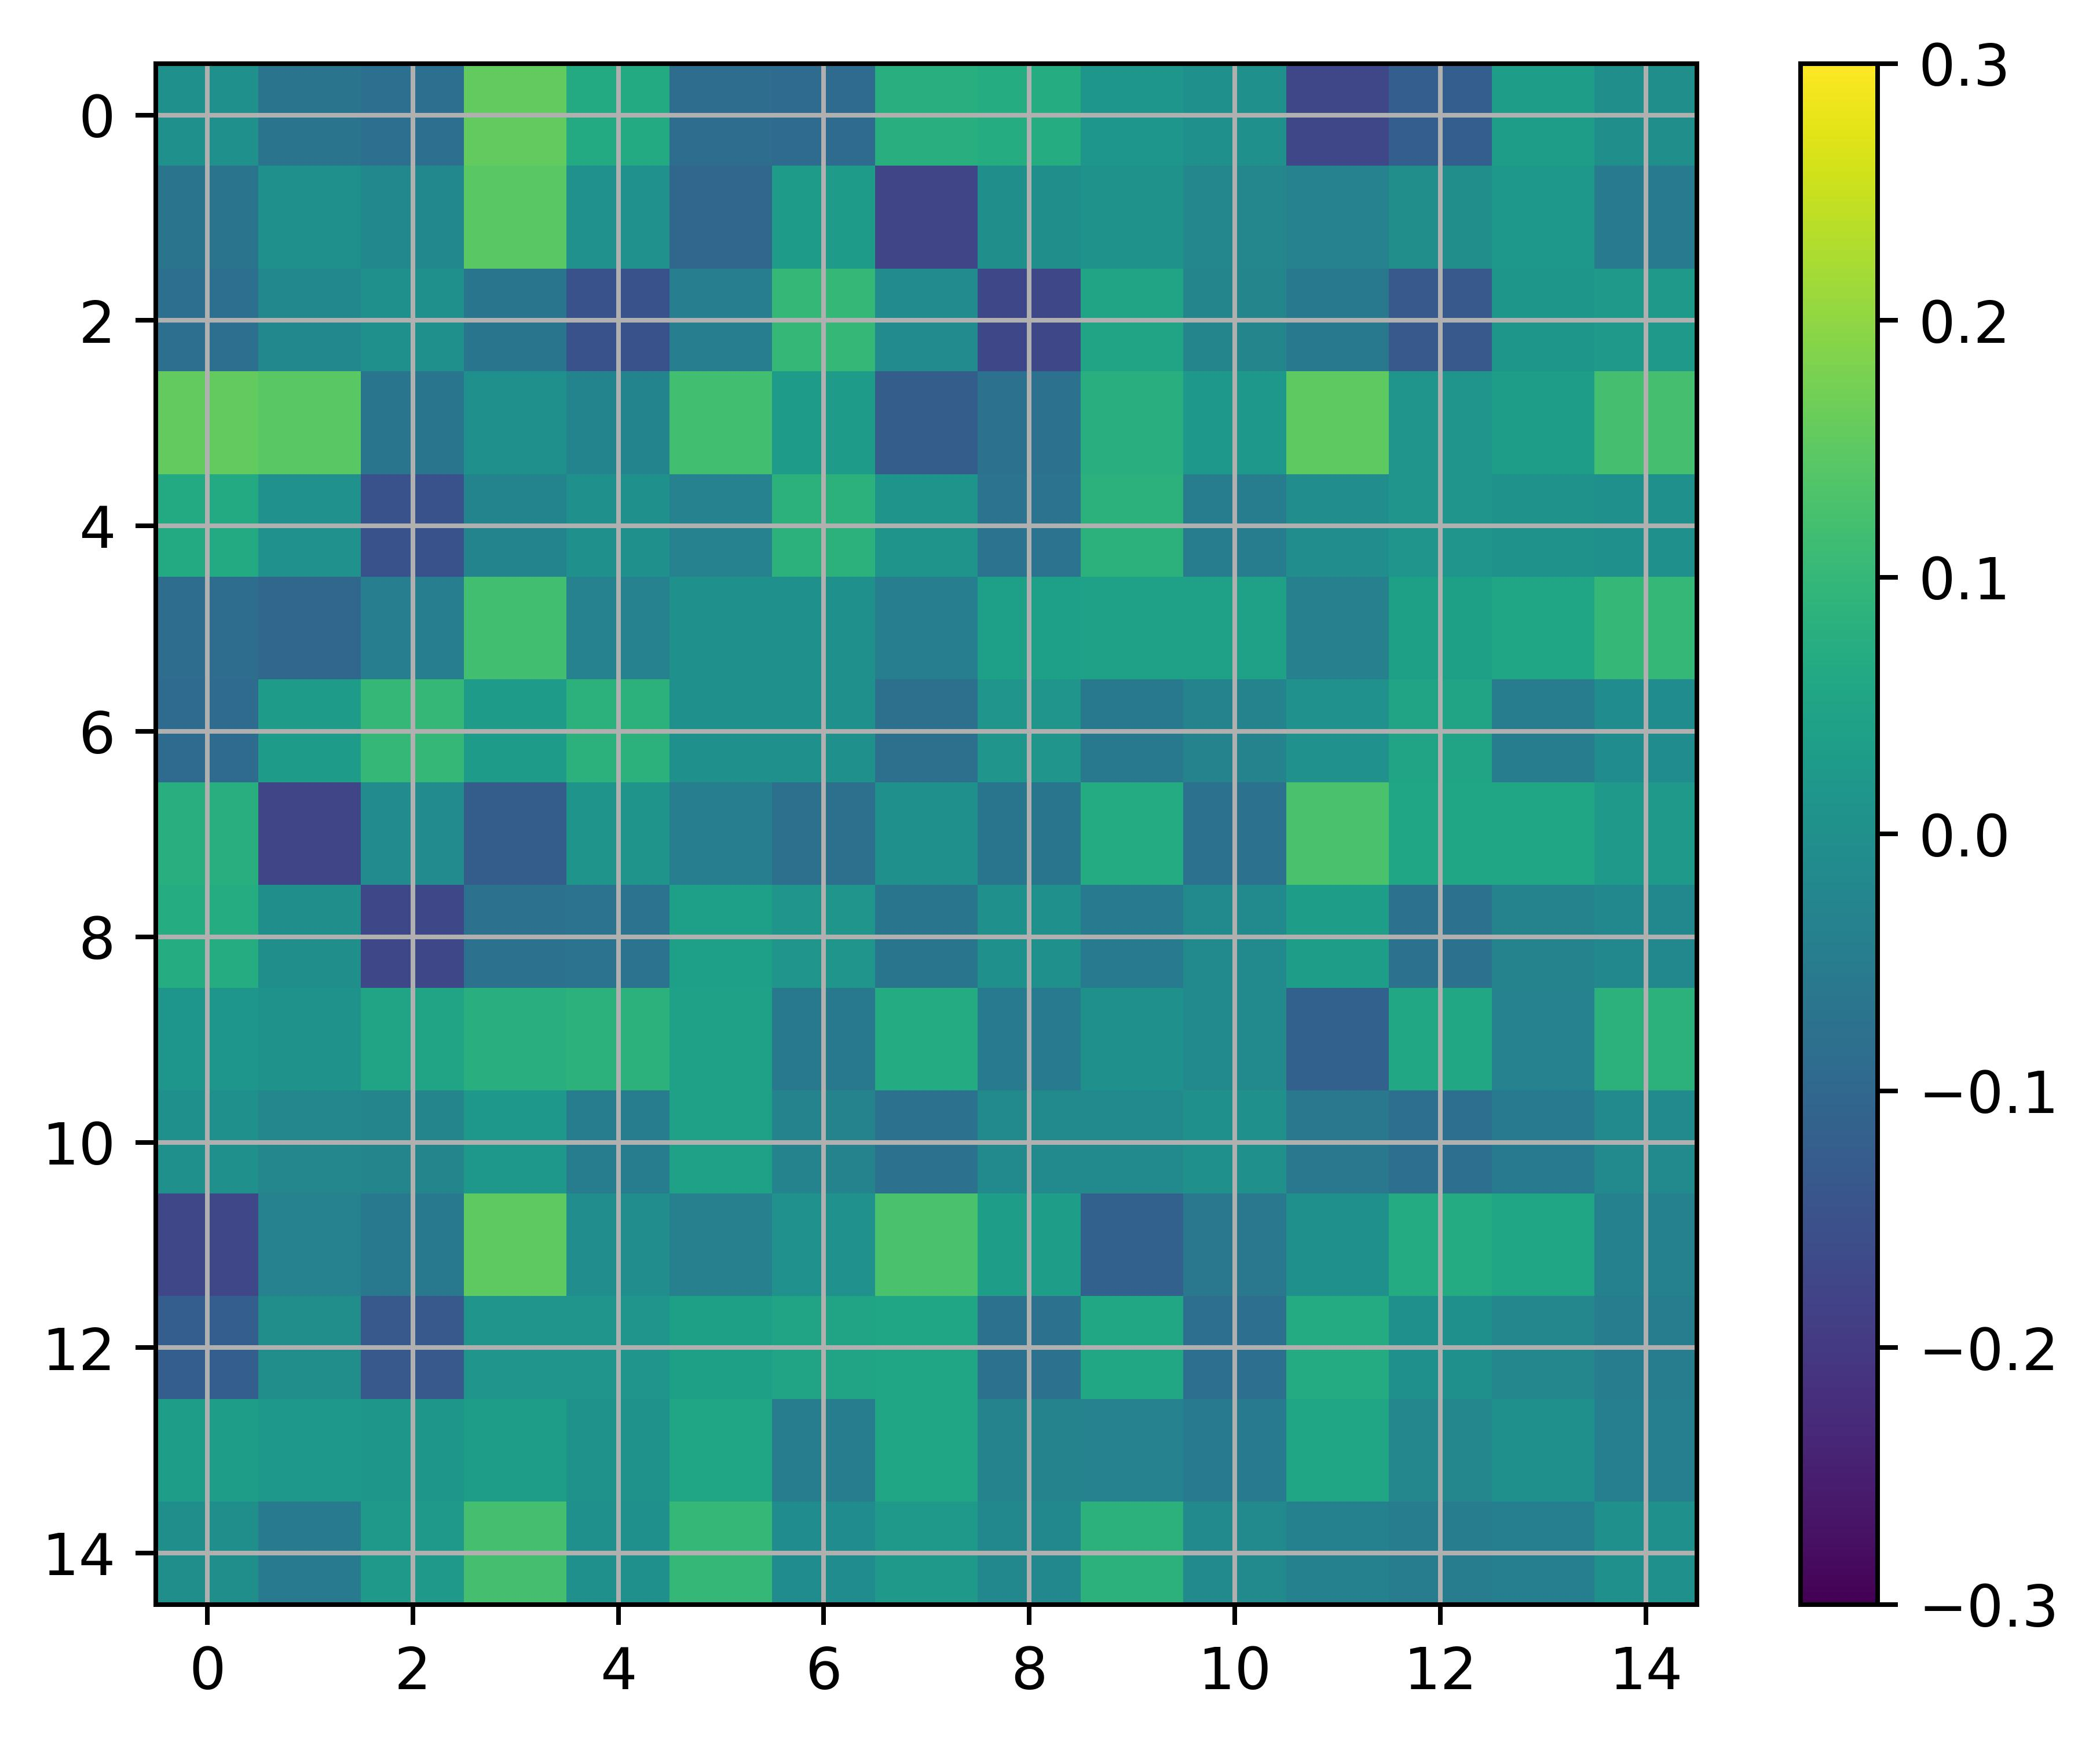
\includegraphics[width=0.2\textwidth]{../Analysis/DFC/size=480_step=180_rho=0.1/node=15_id=100206/c_4.jpg}
        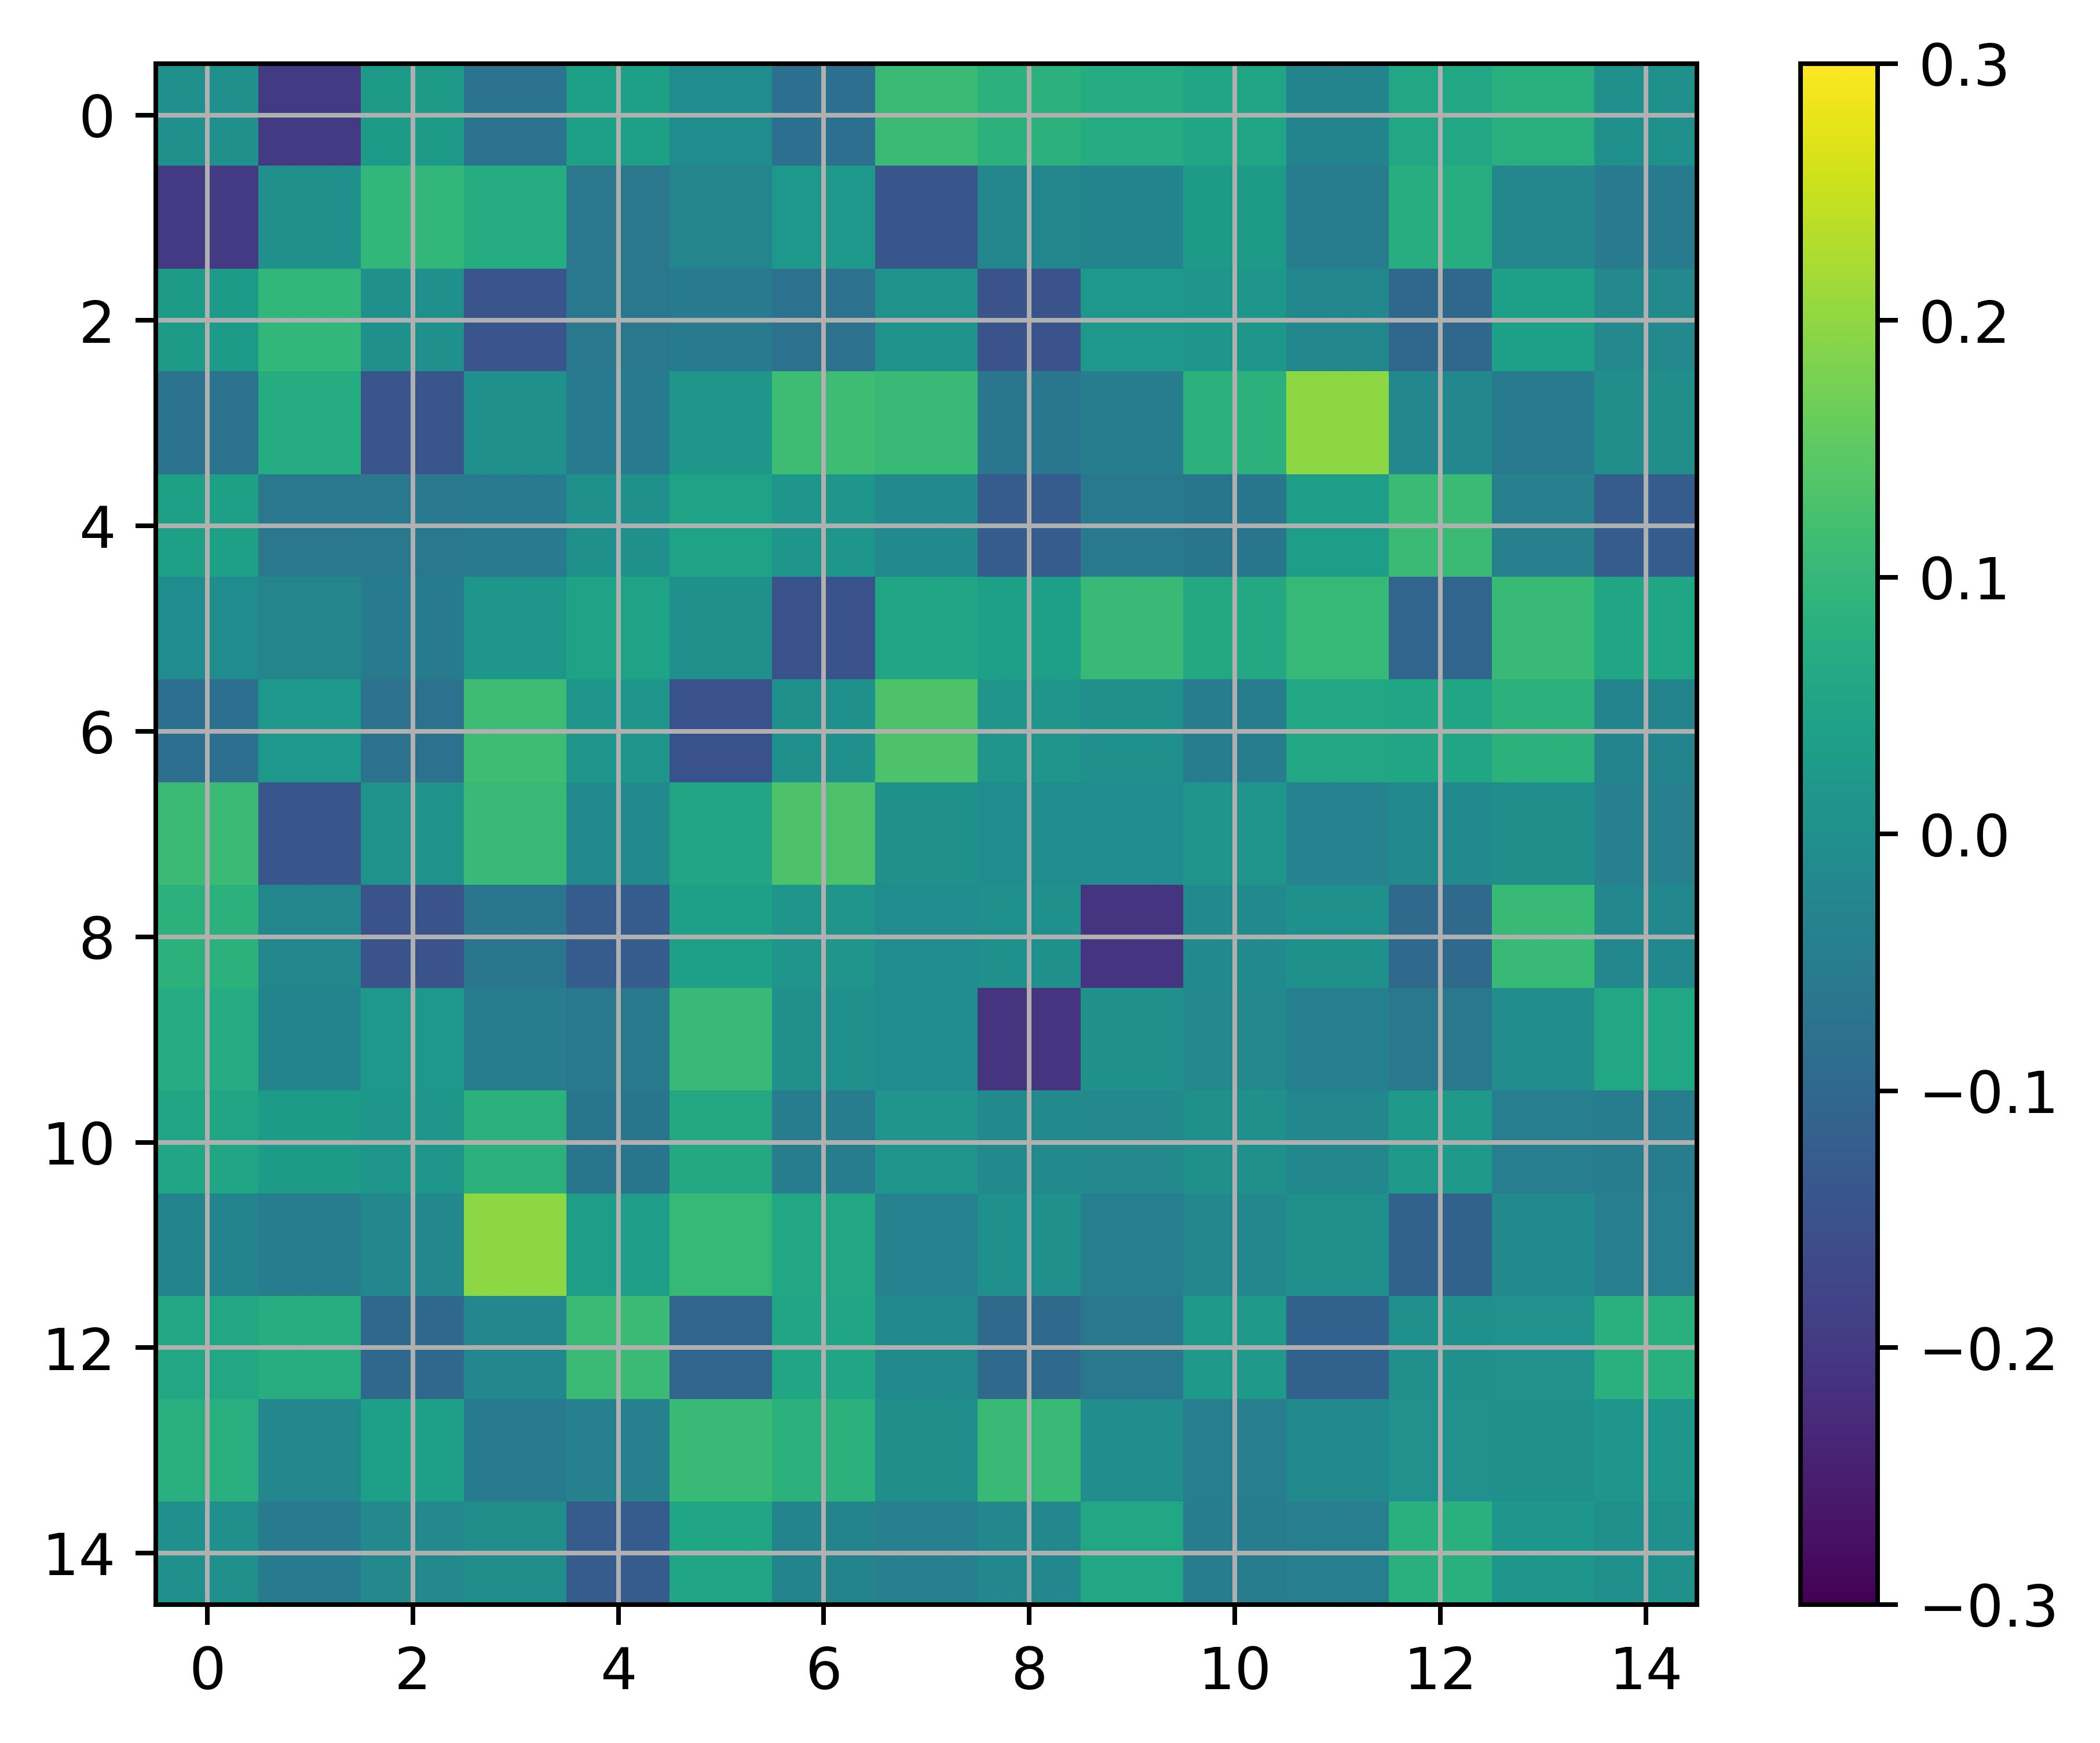
\includegraphics[width=0.2\textwidth]{../Analysis/DFC/size=480_step=180_rho=0.1/node=15_id=100206/c_6.jpg} \\
        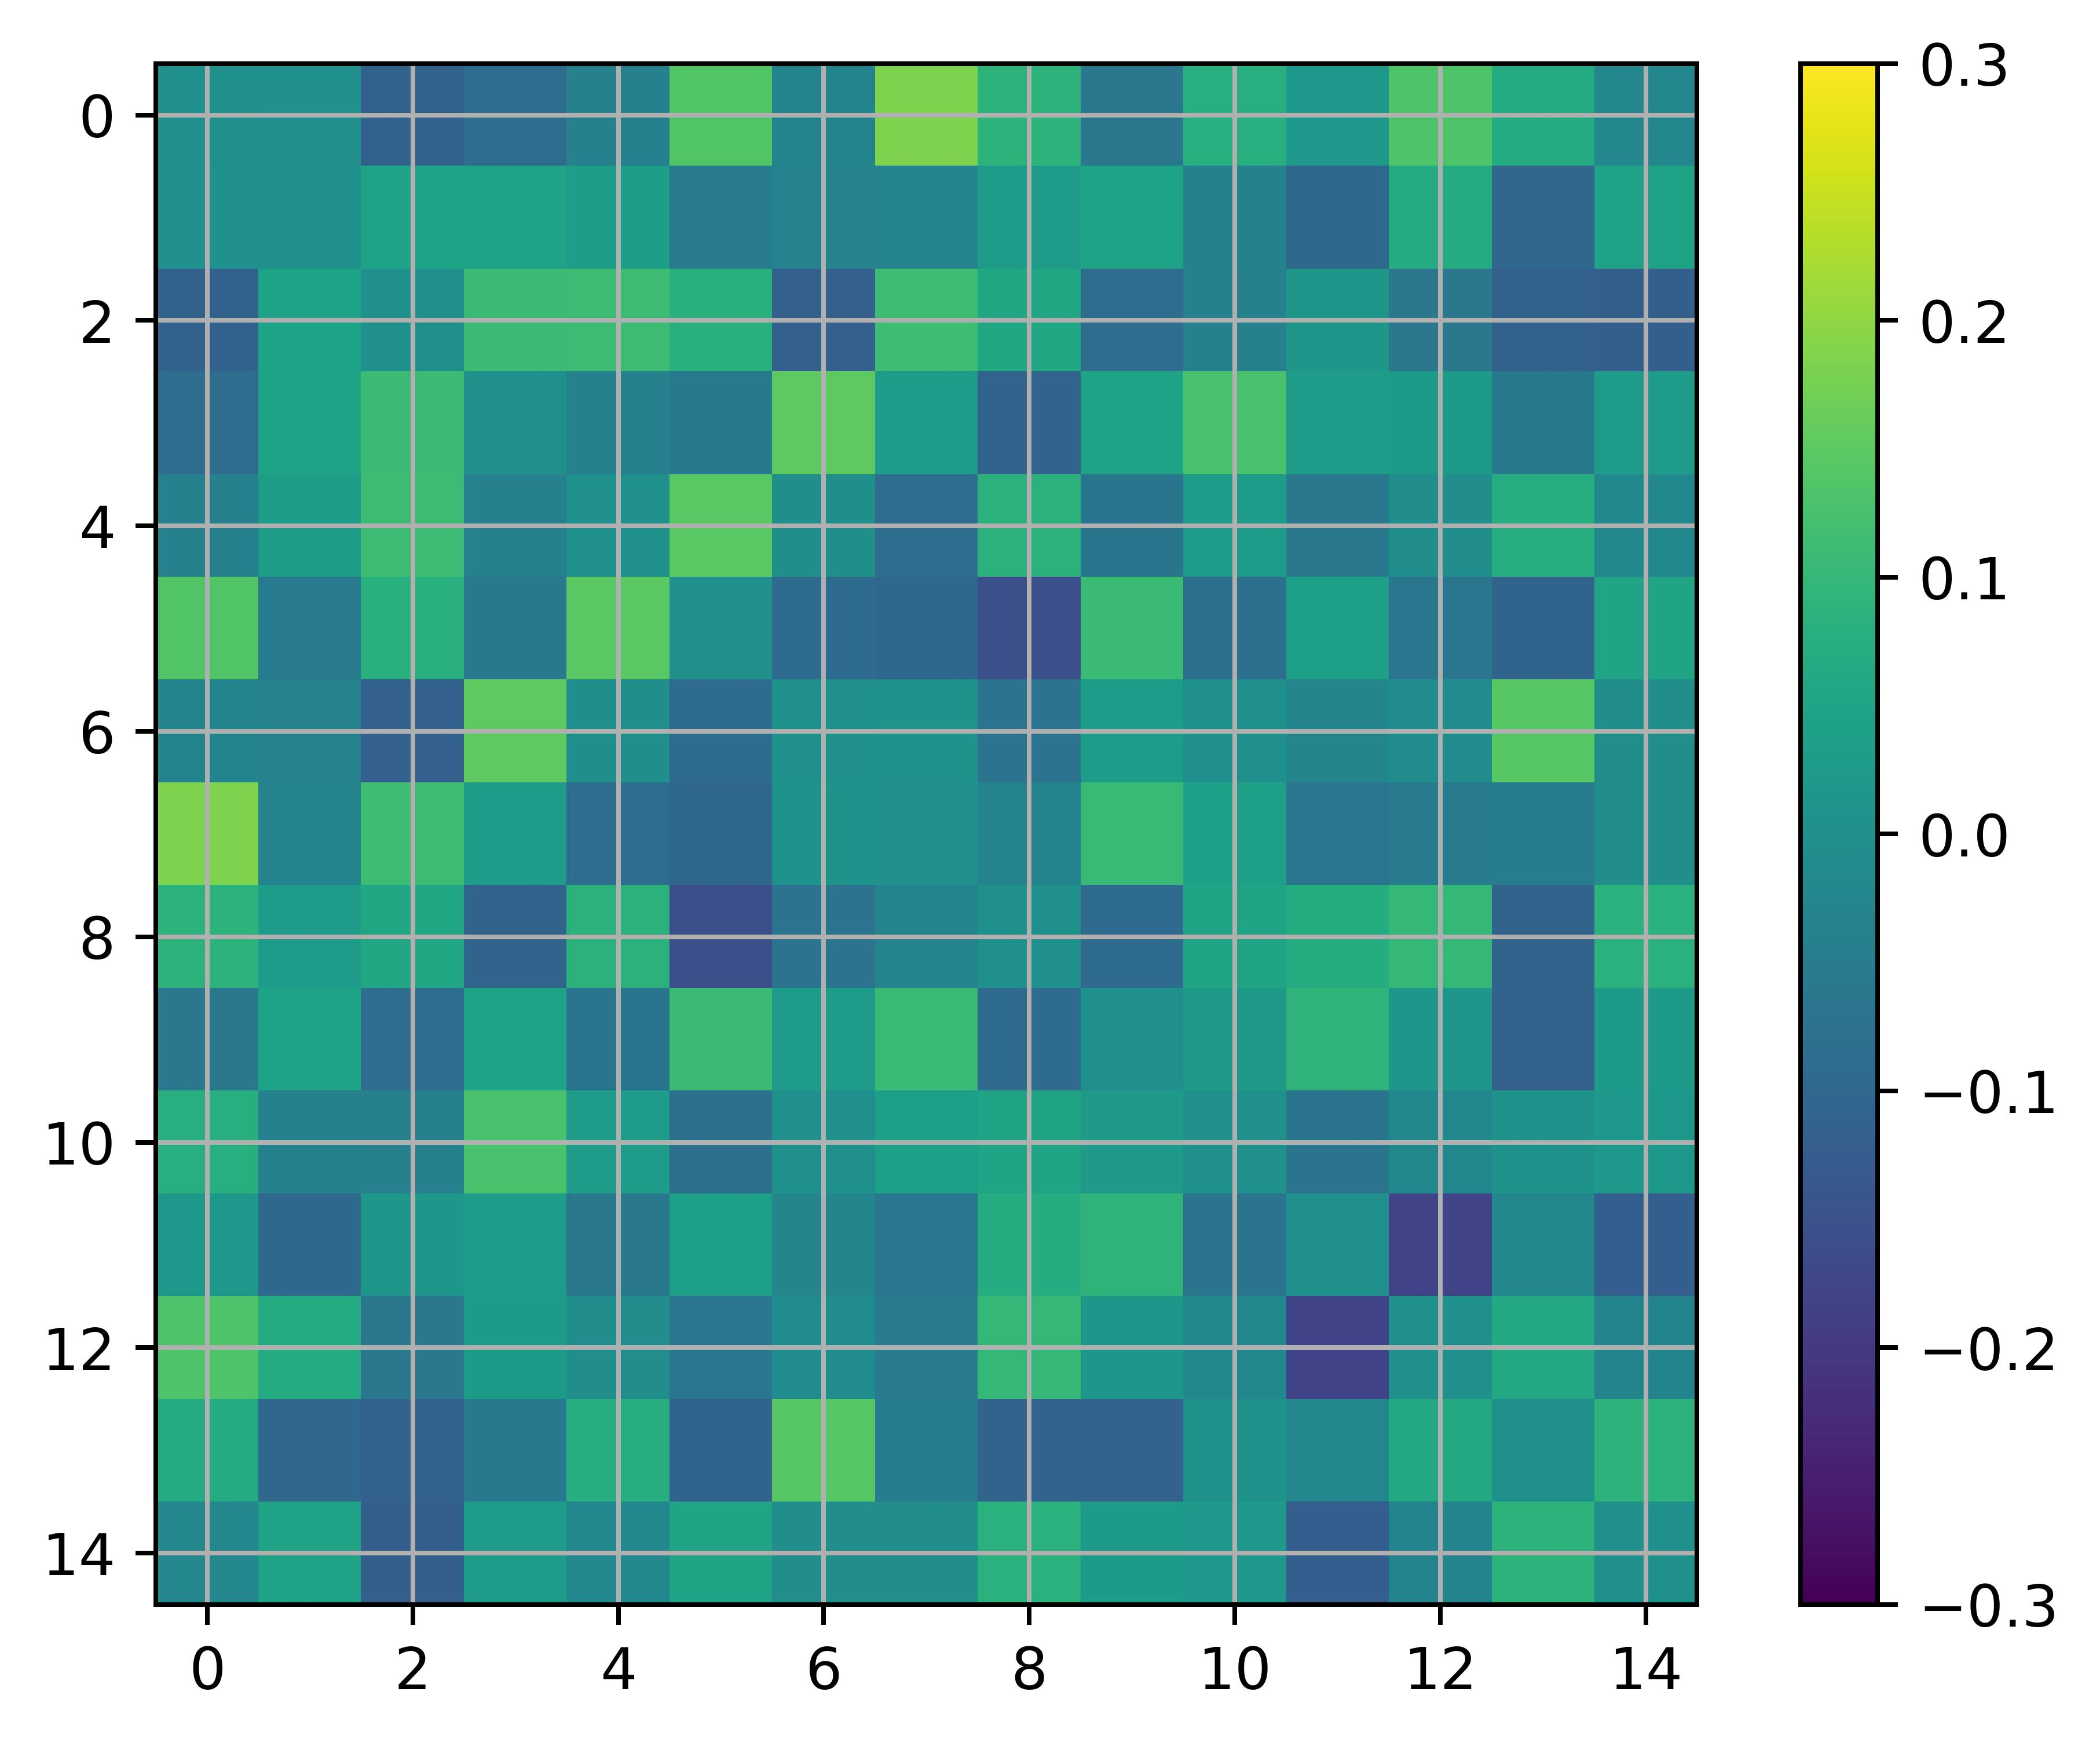
\includegraphics[width=0.2\textwidth]{../Analysis/DFC/size=480_step=180_rho=0.1/node=15_id=100206/c_8.jpg}
        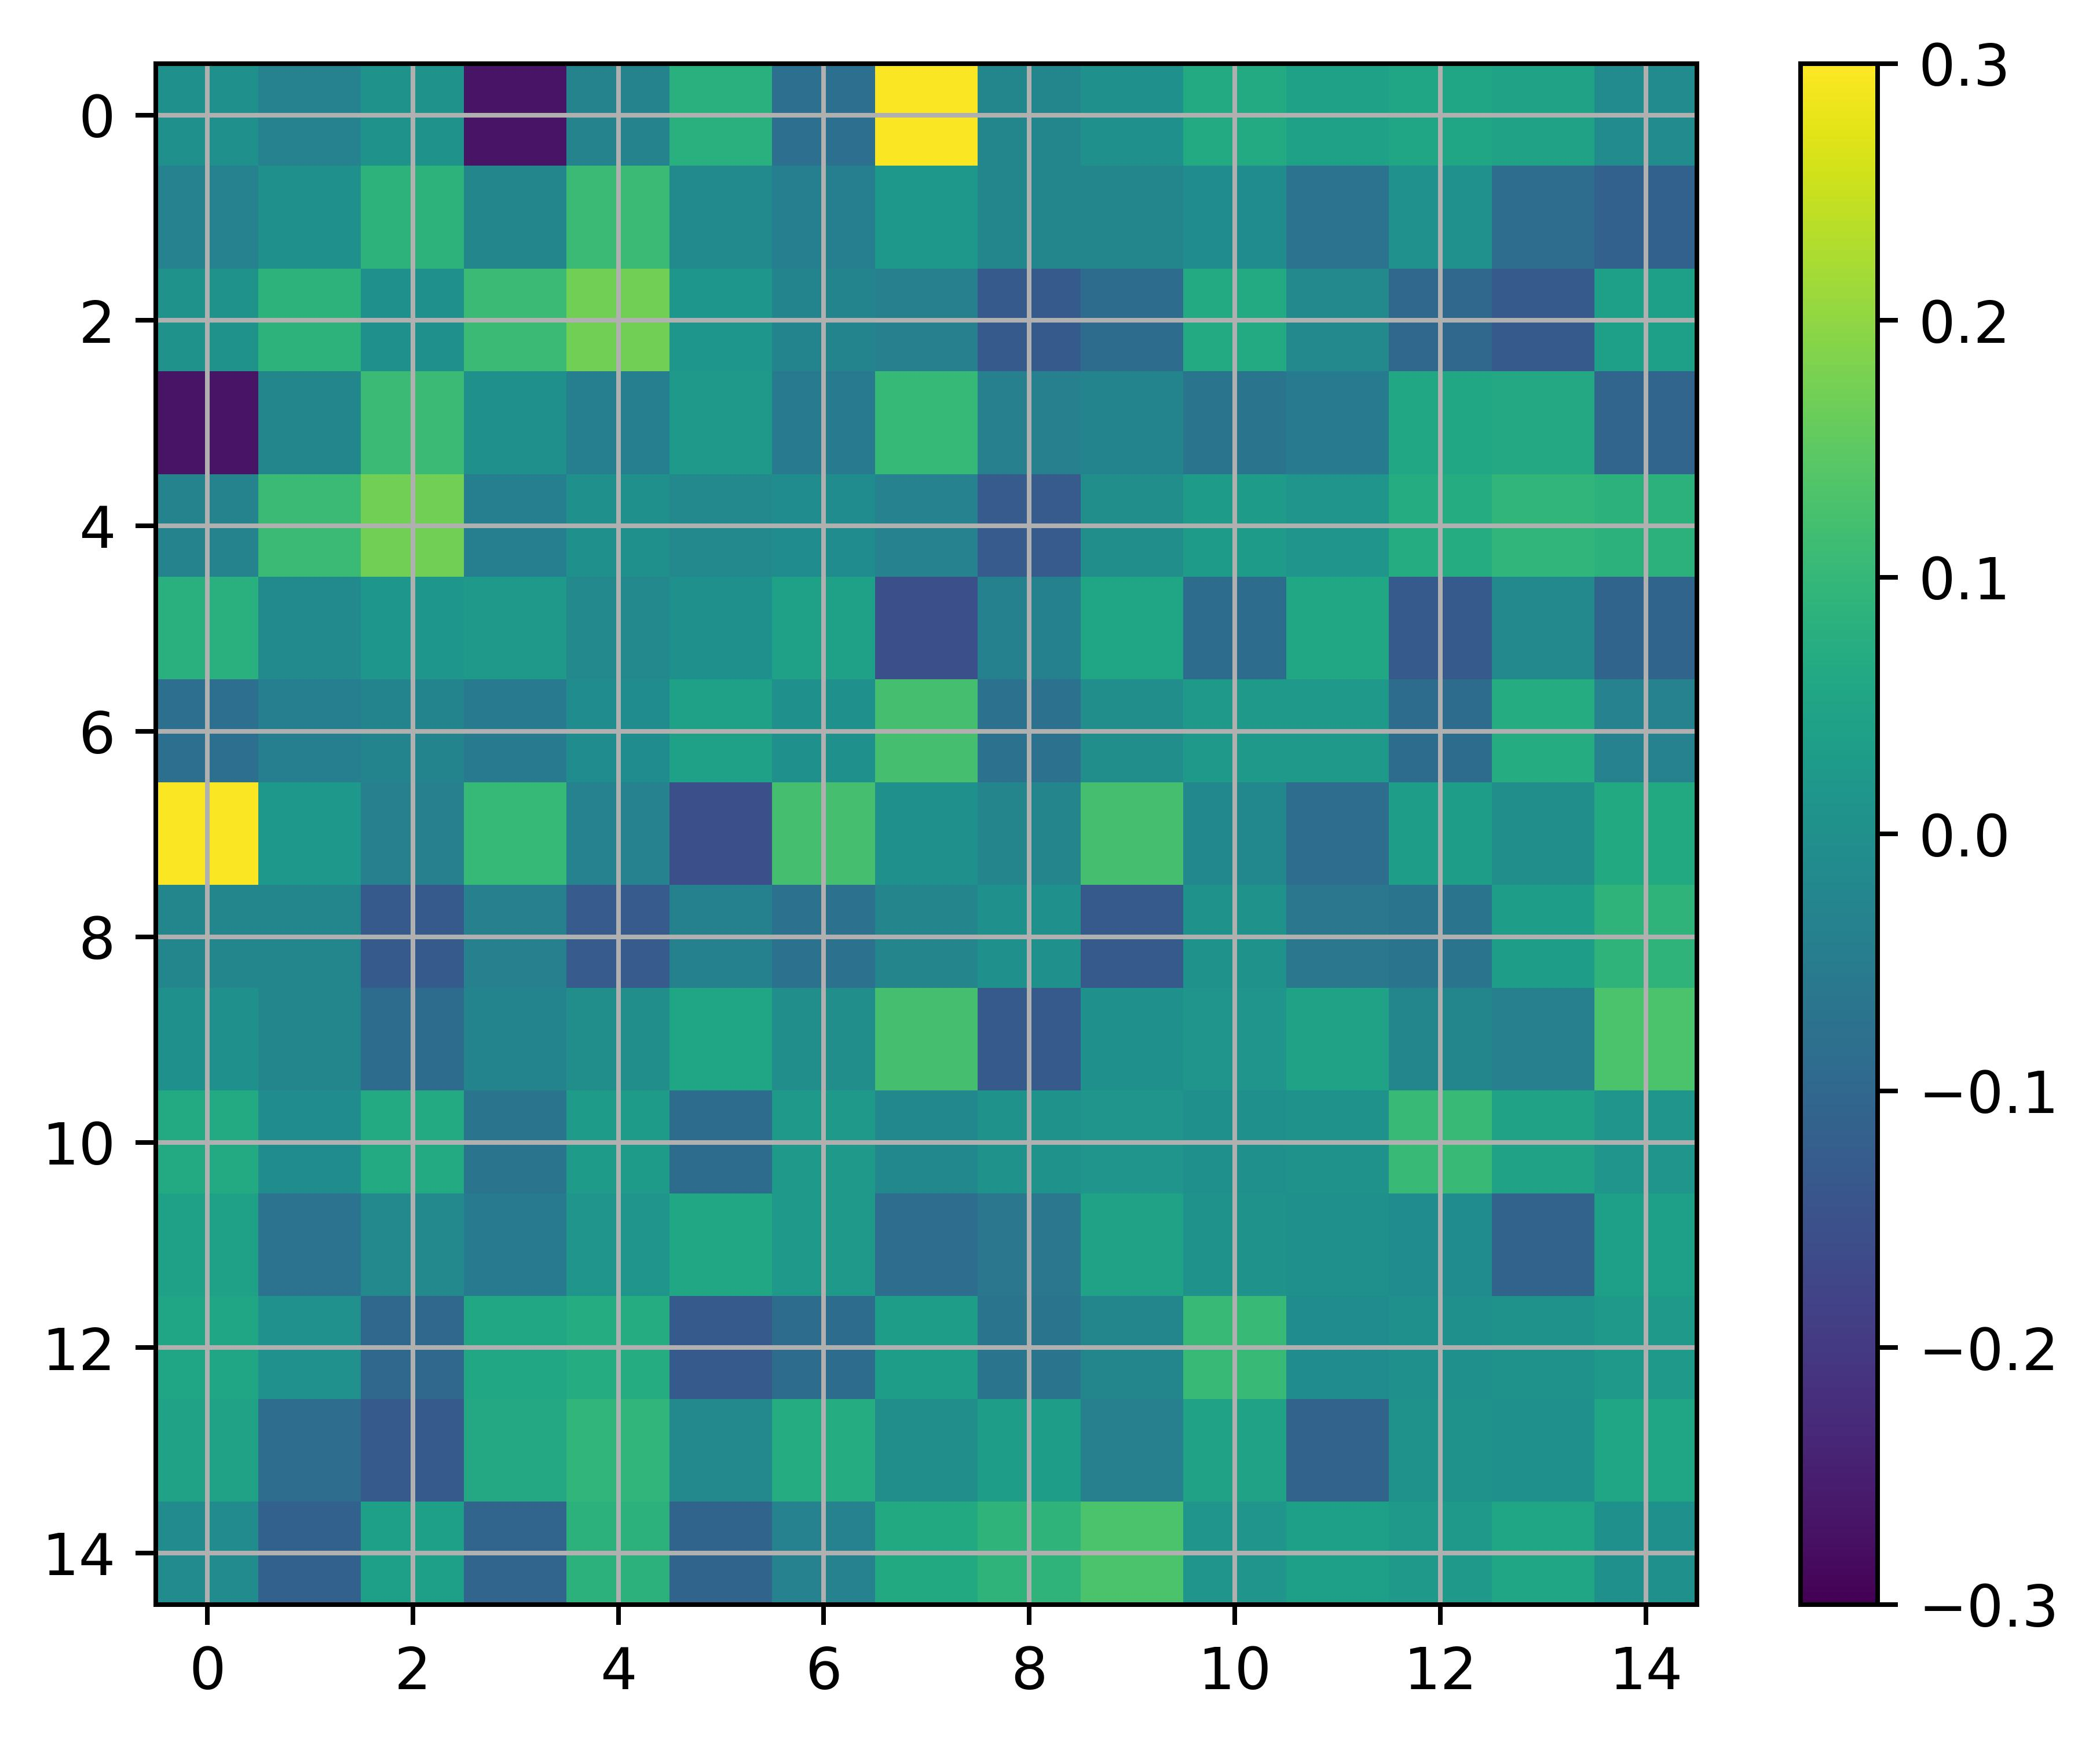
\includegraphics[width=0.2\textwidth]{../Analysis/DFC/size=480_step=180_rho=0.1/node=15_id=100206/c_10.jpg}
        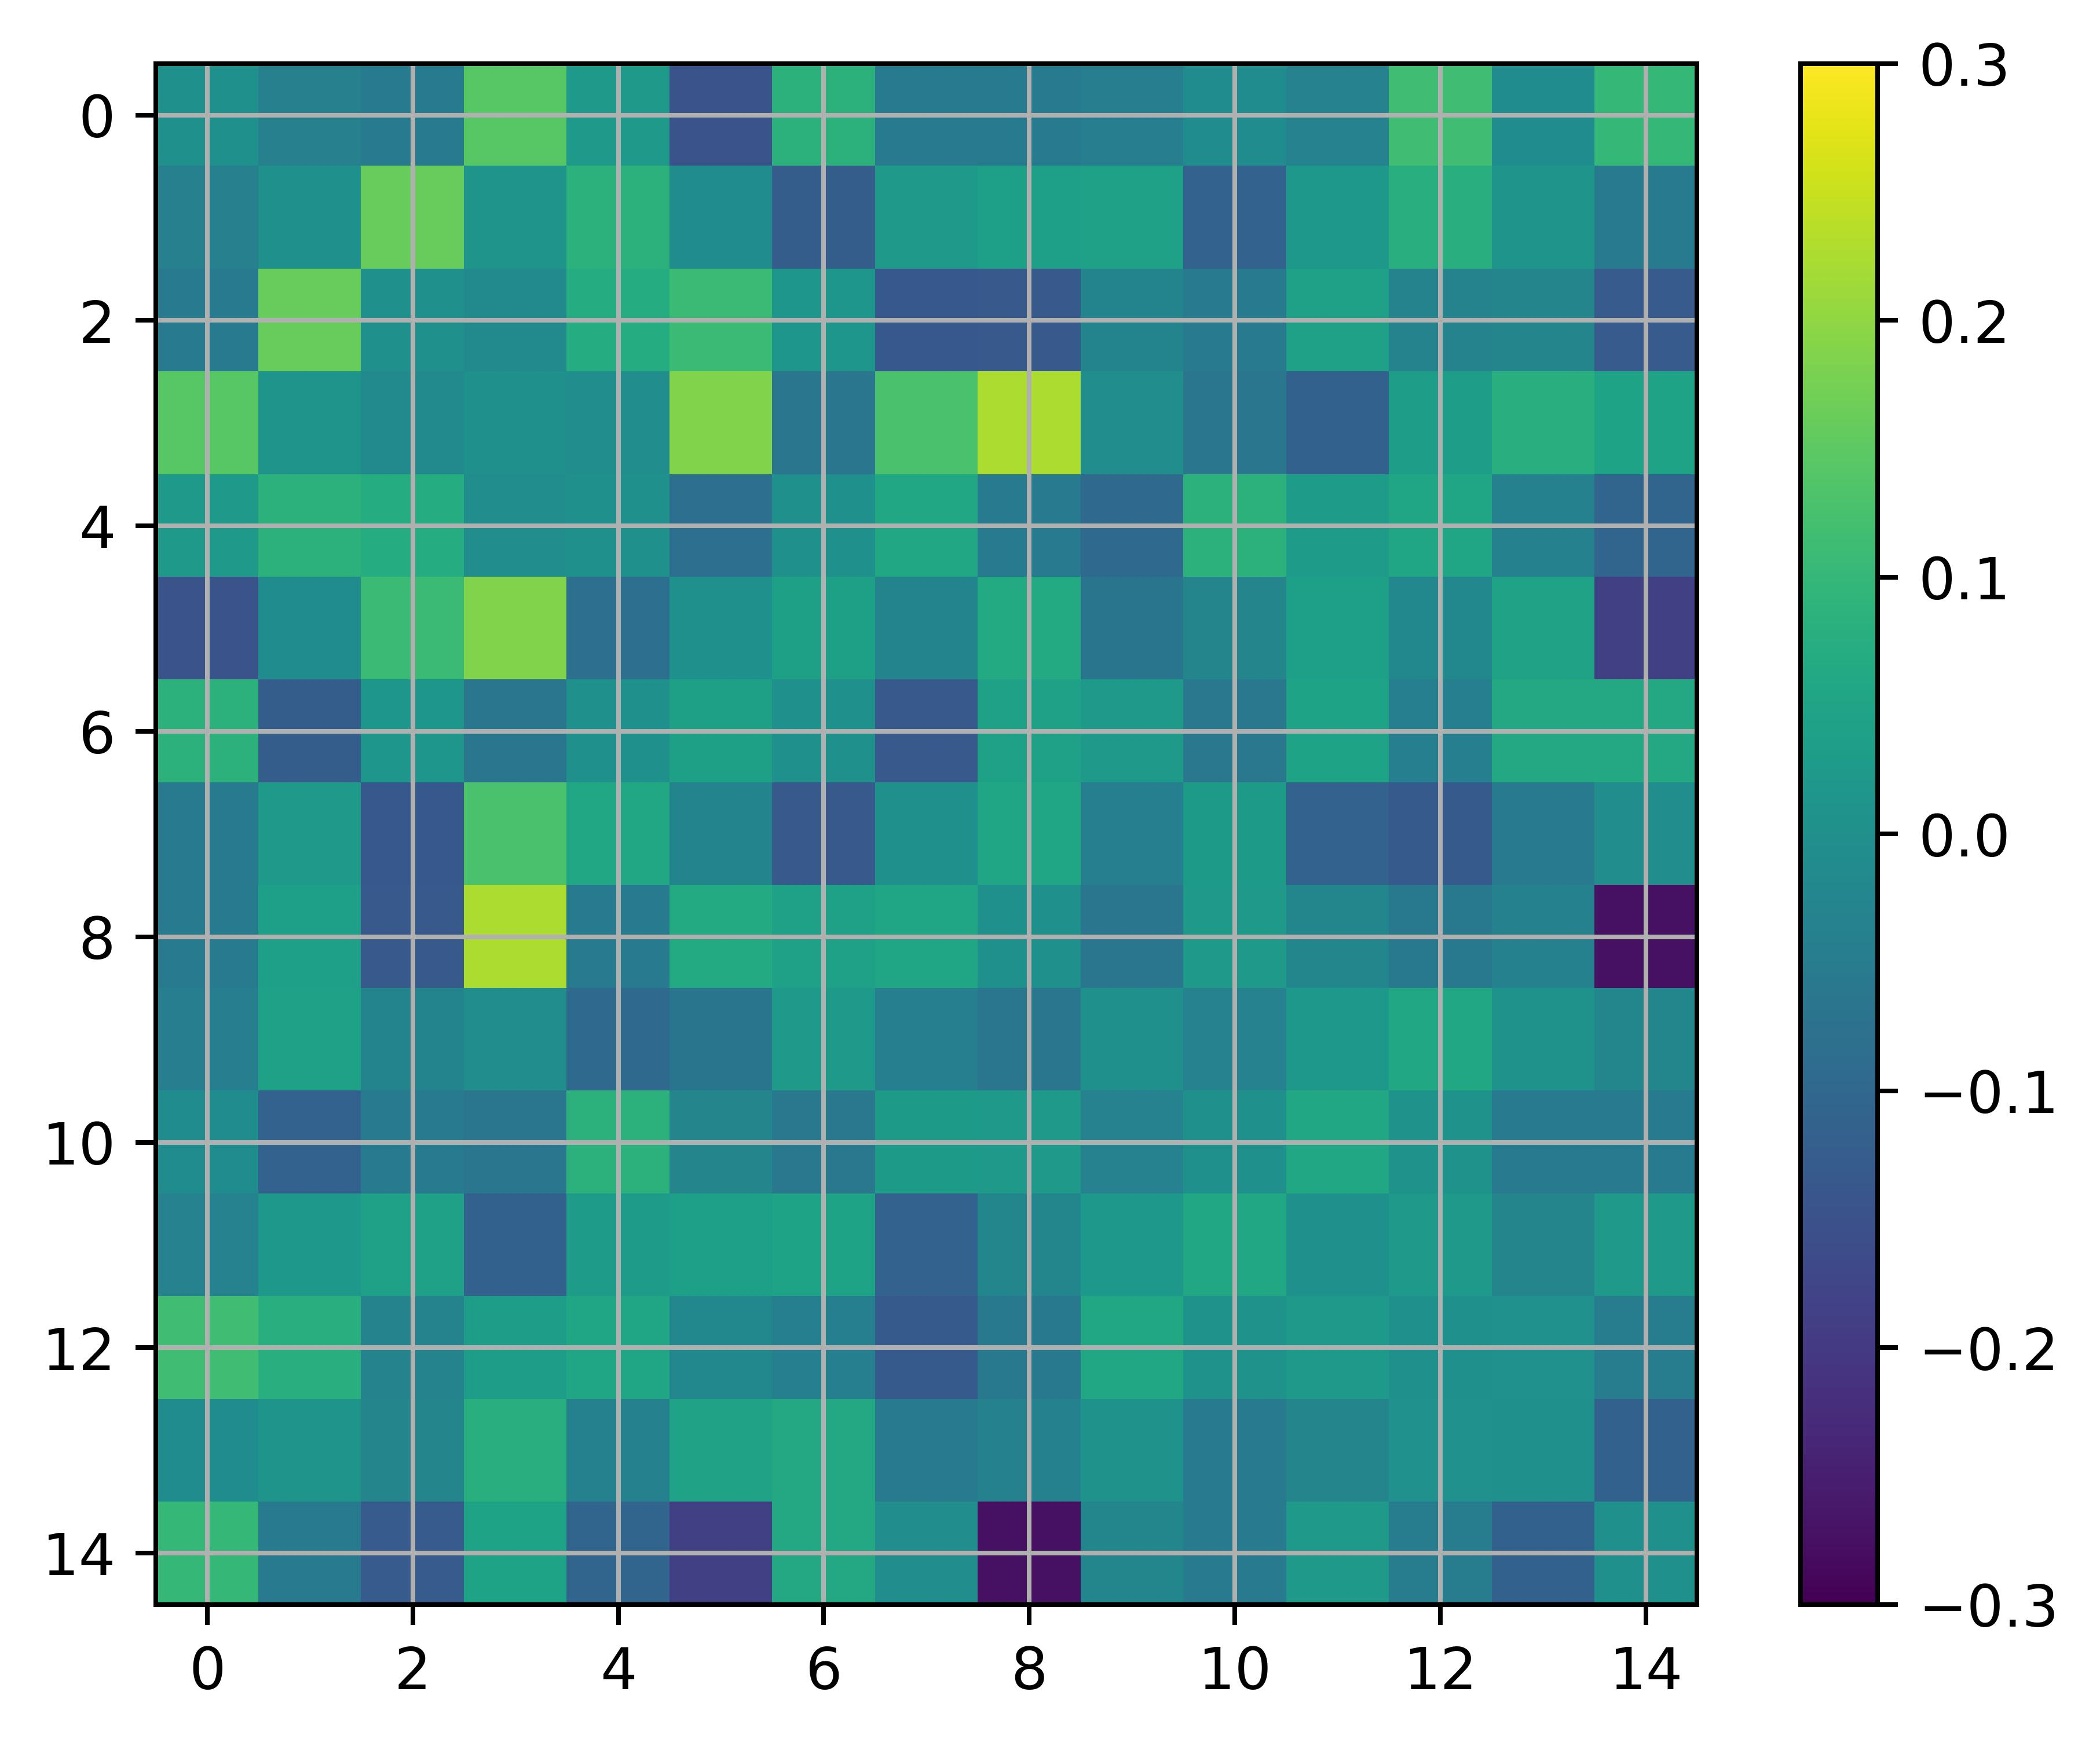
\includegraphics[width=0.2\textwidth]{../Analysis/DFC/size=480_step=180_rho=0.1/node=15_id=100206/c_12.jpg}
        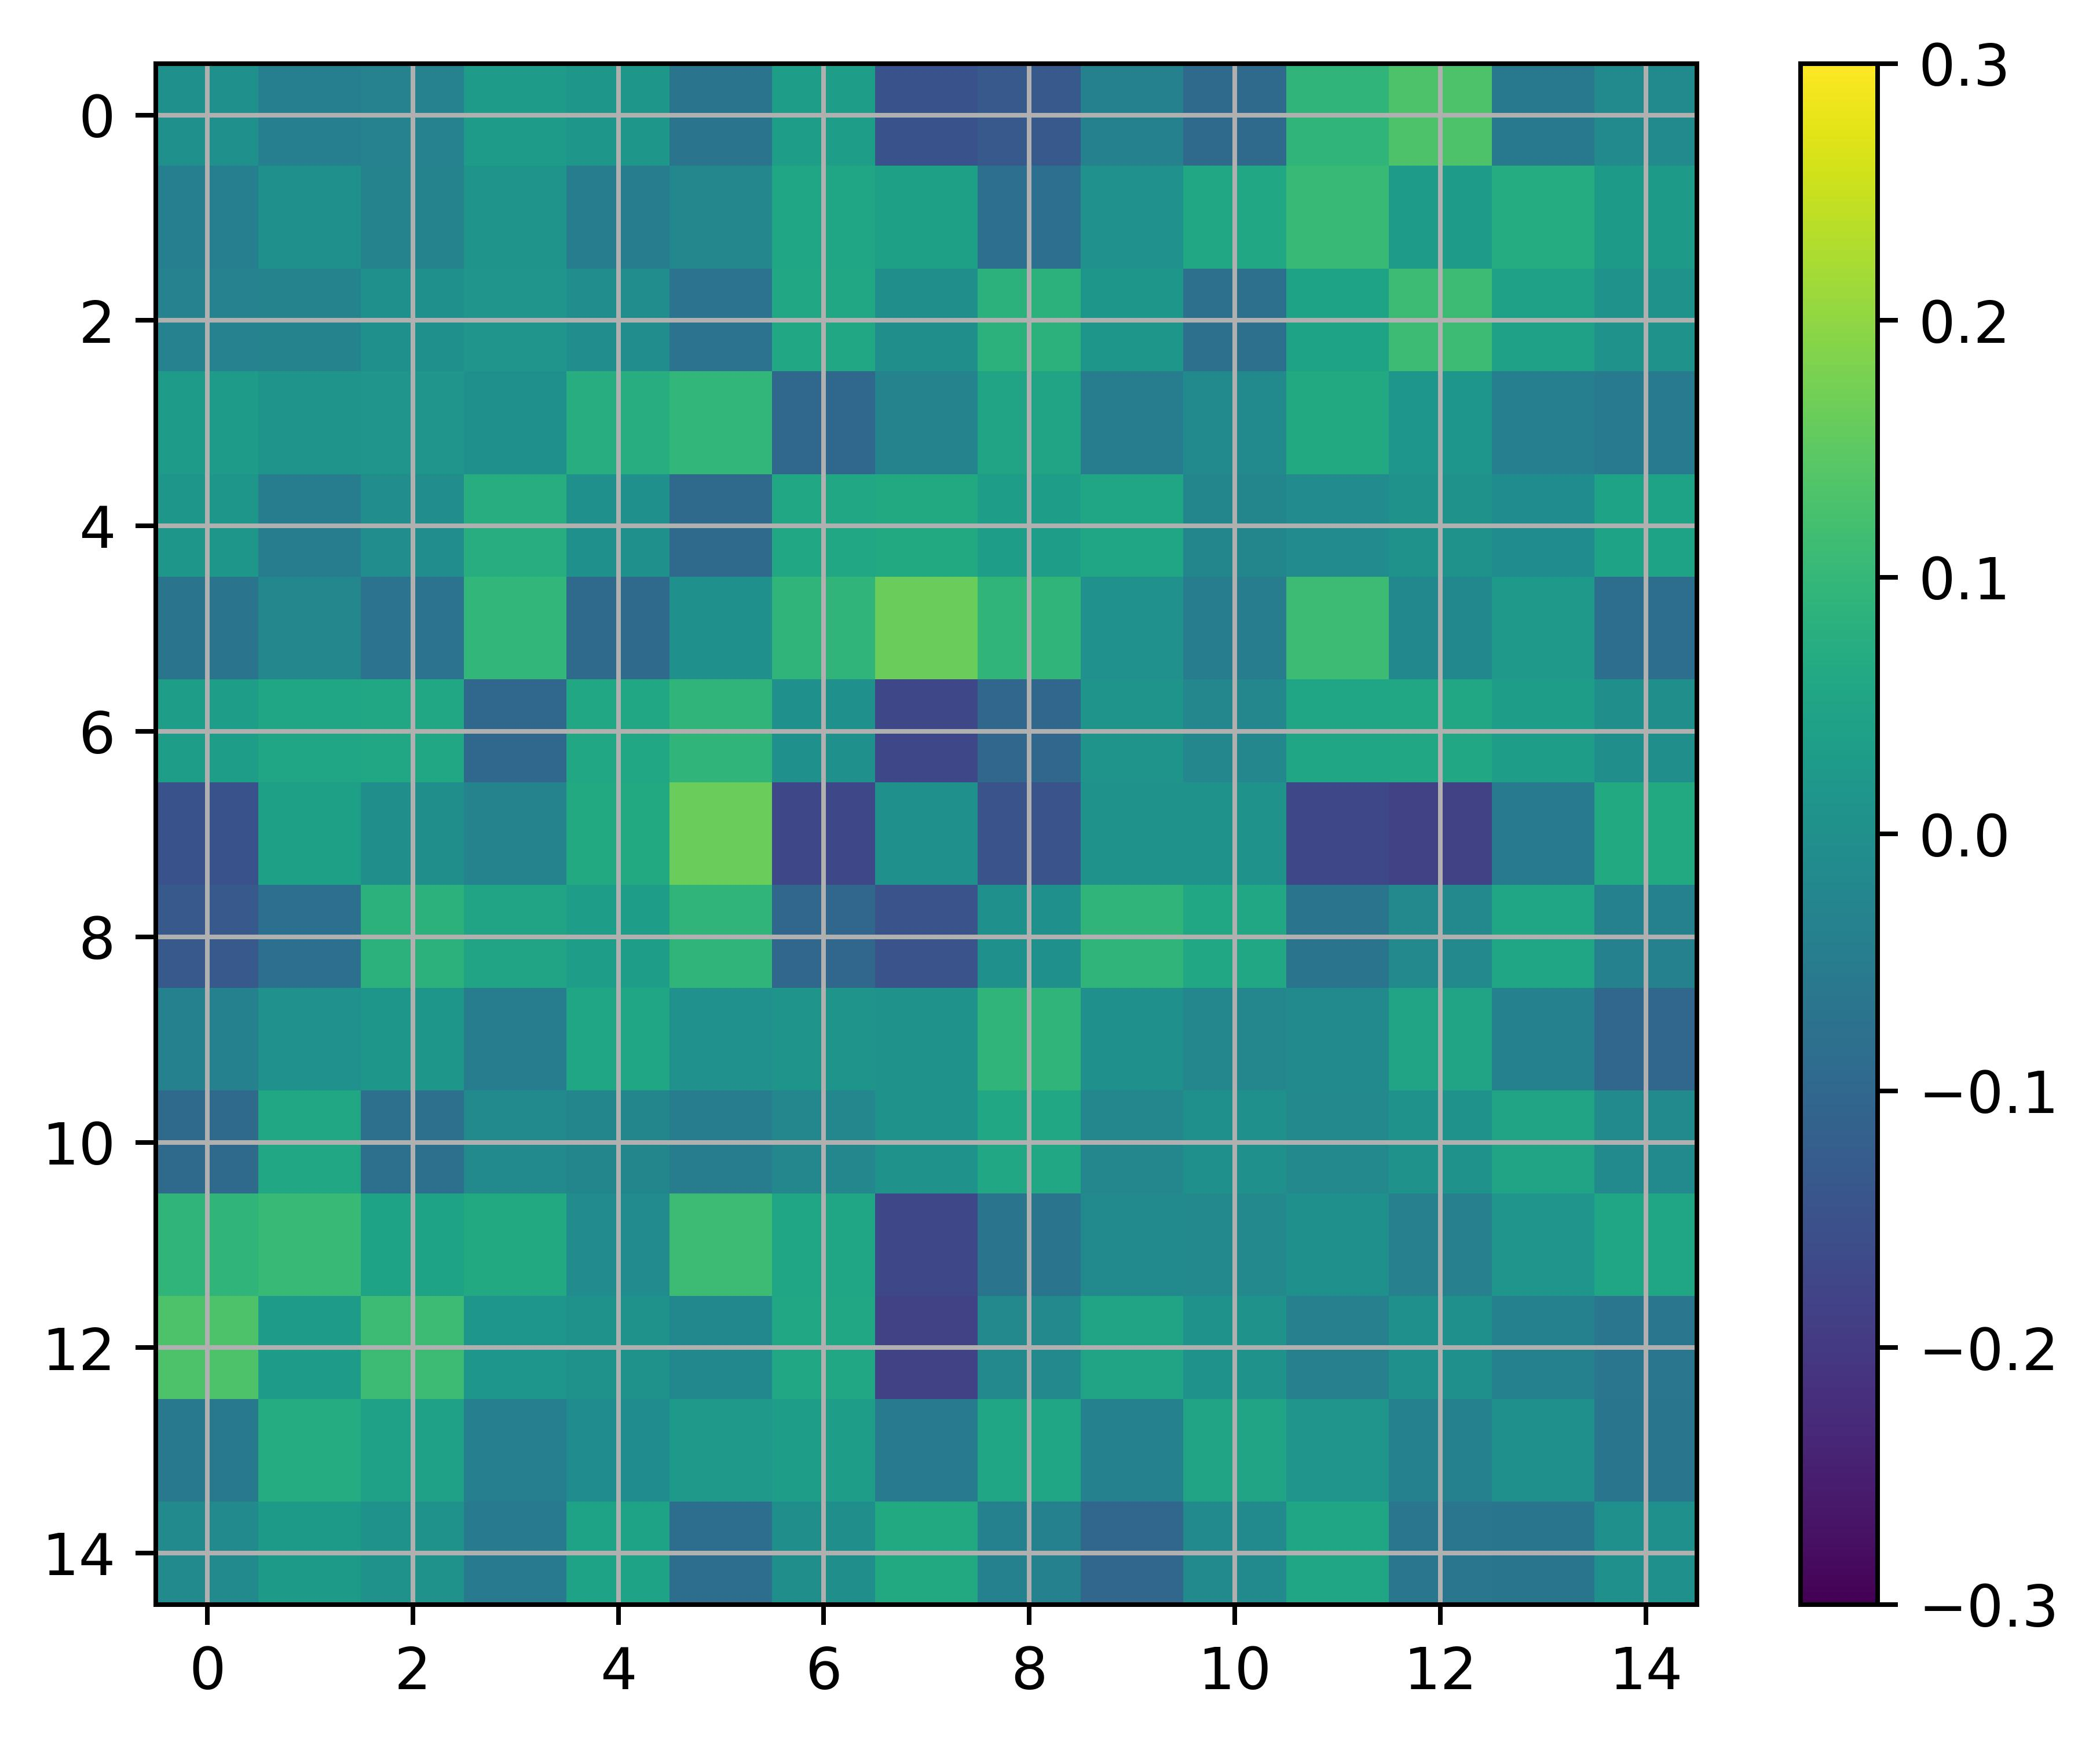
\includegraphics[width=0.2\textwidth]{../Analysis/DFC/size=480_step=180_rho=0.1/node=15_id=100206/c_14.jpg} \\
        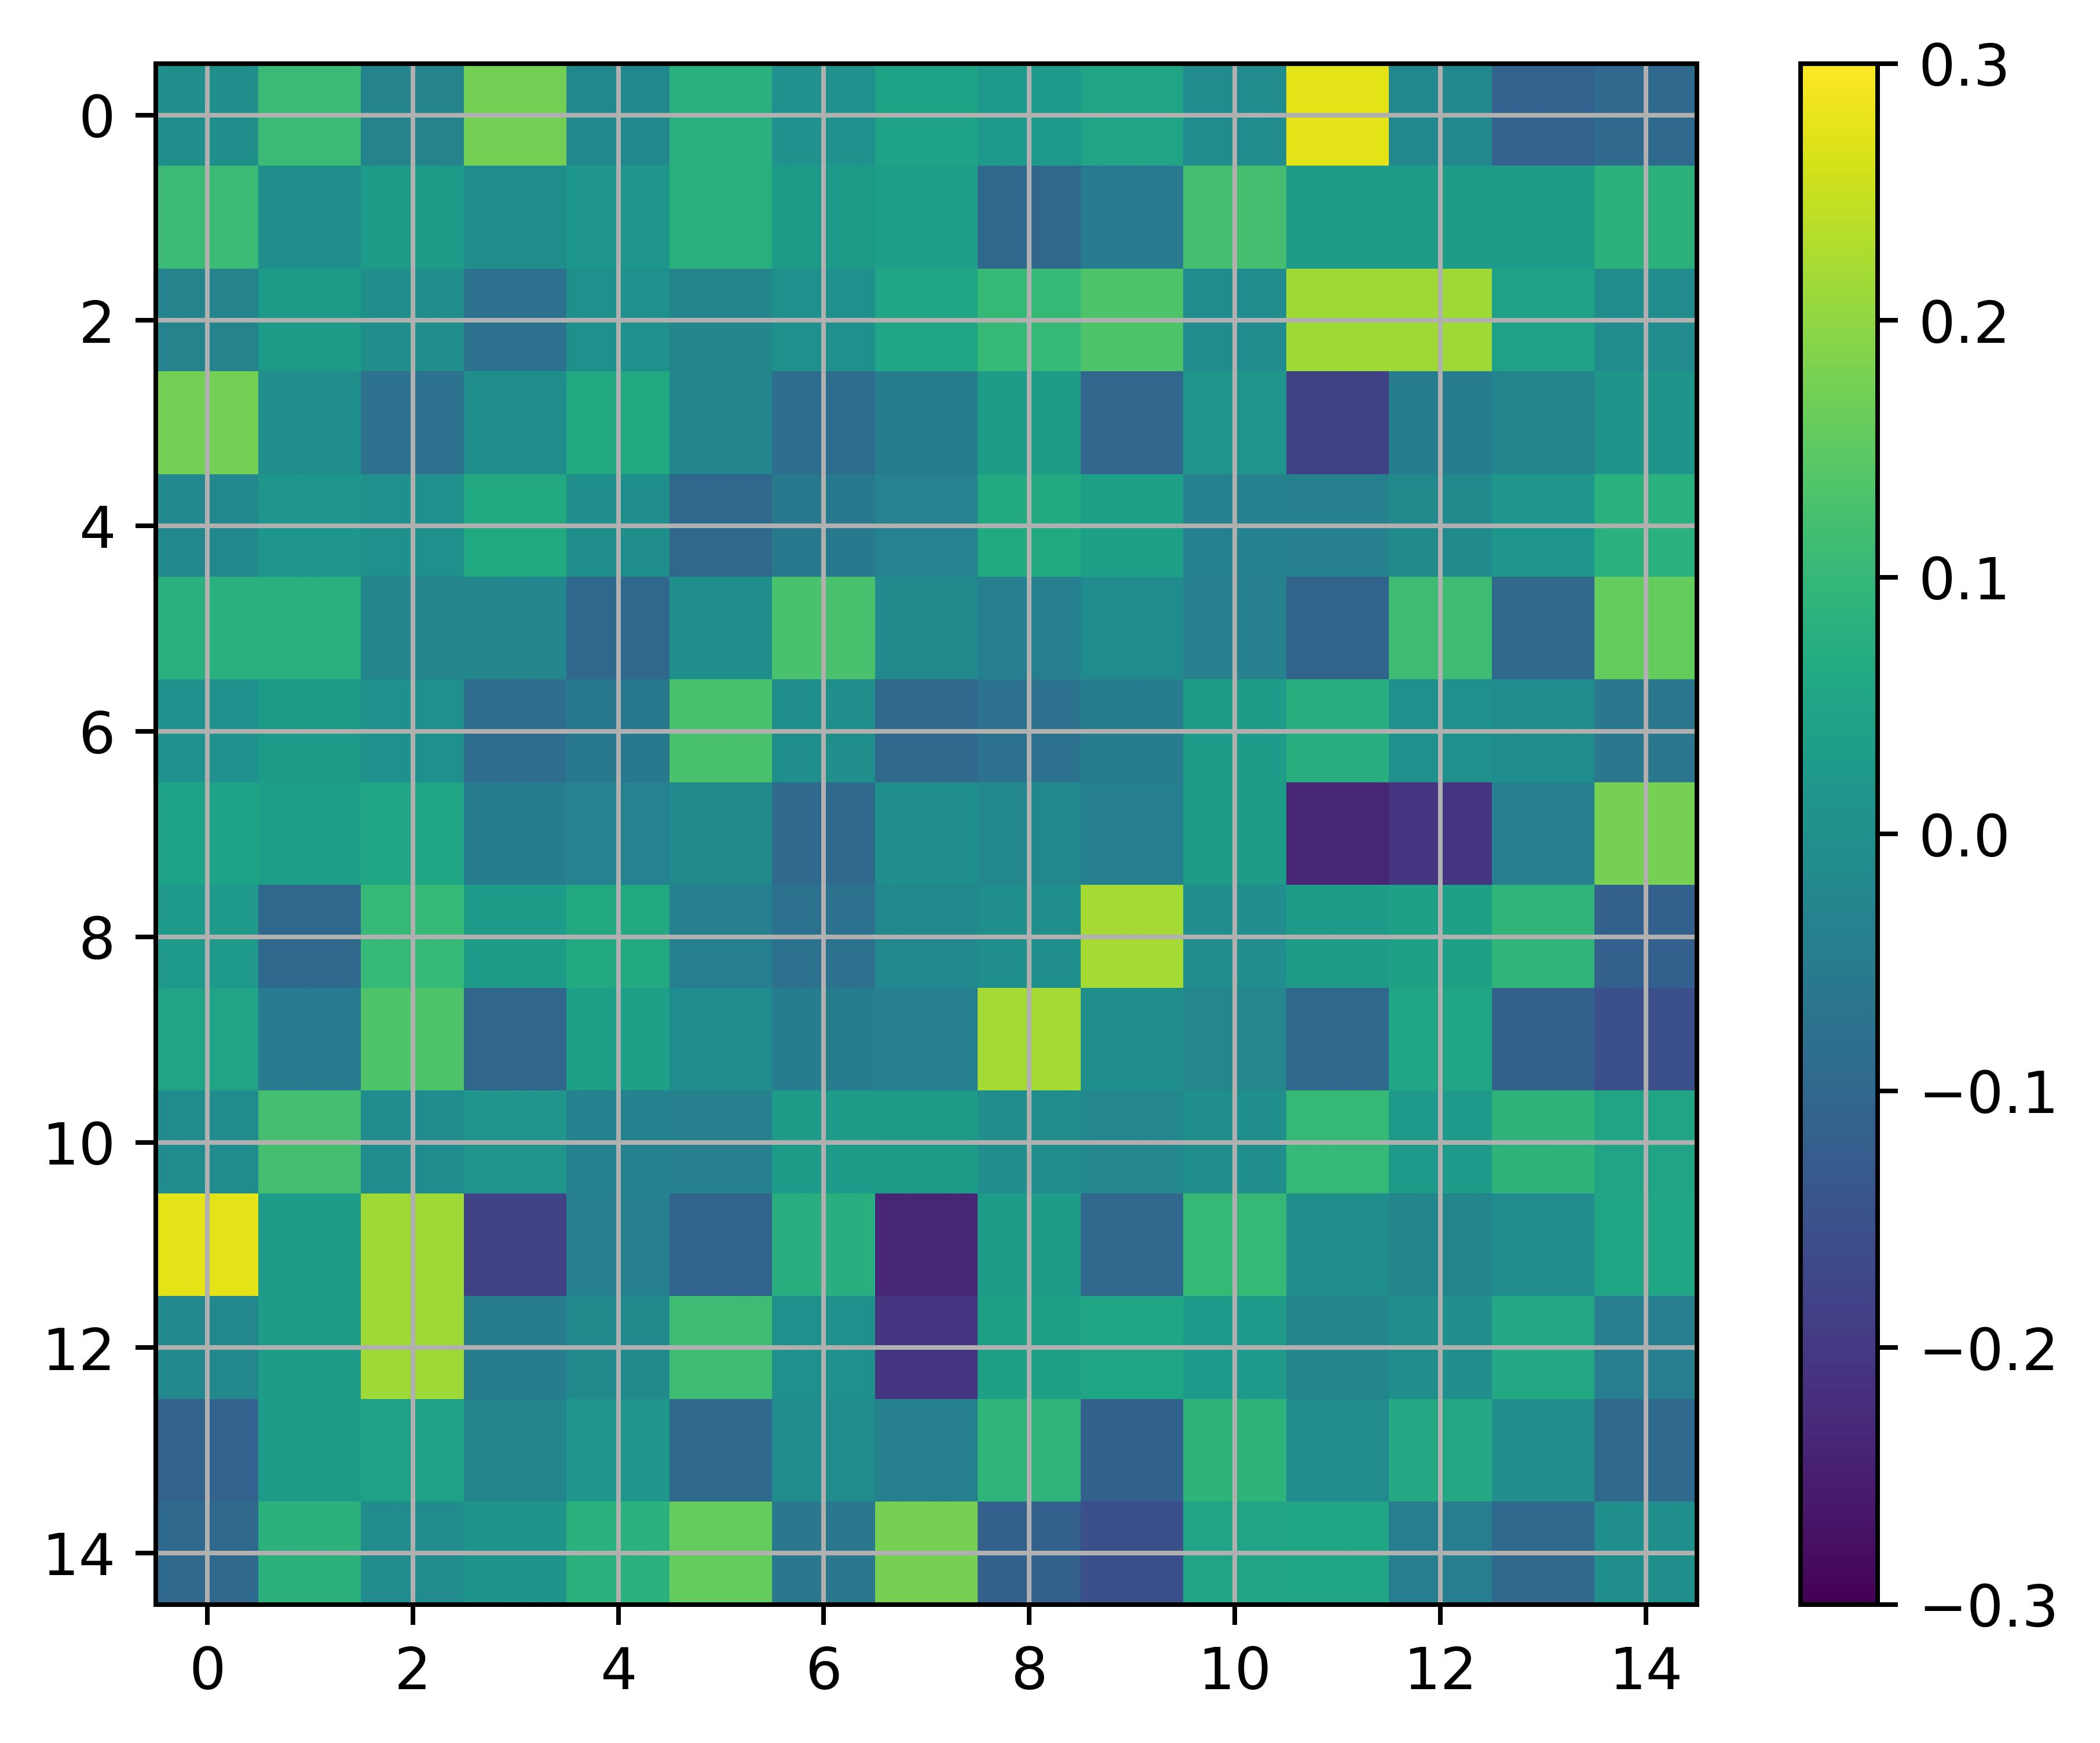
\includegraphics[width=0.2\textwidth]{../Analysis/DFC/size=480_step=180_rho=0.1/node=15_id=100206/c_16.jpg}
        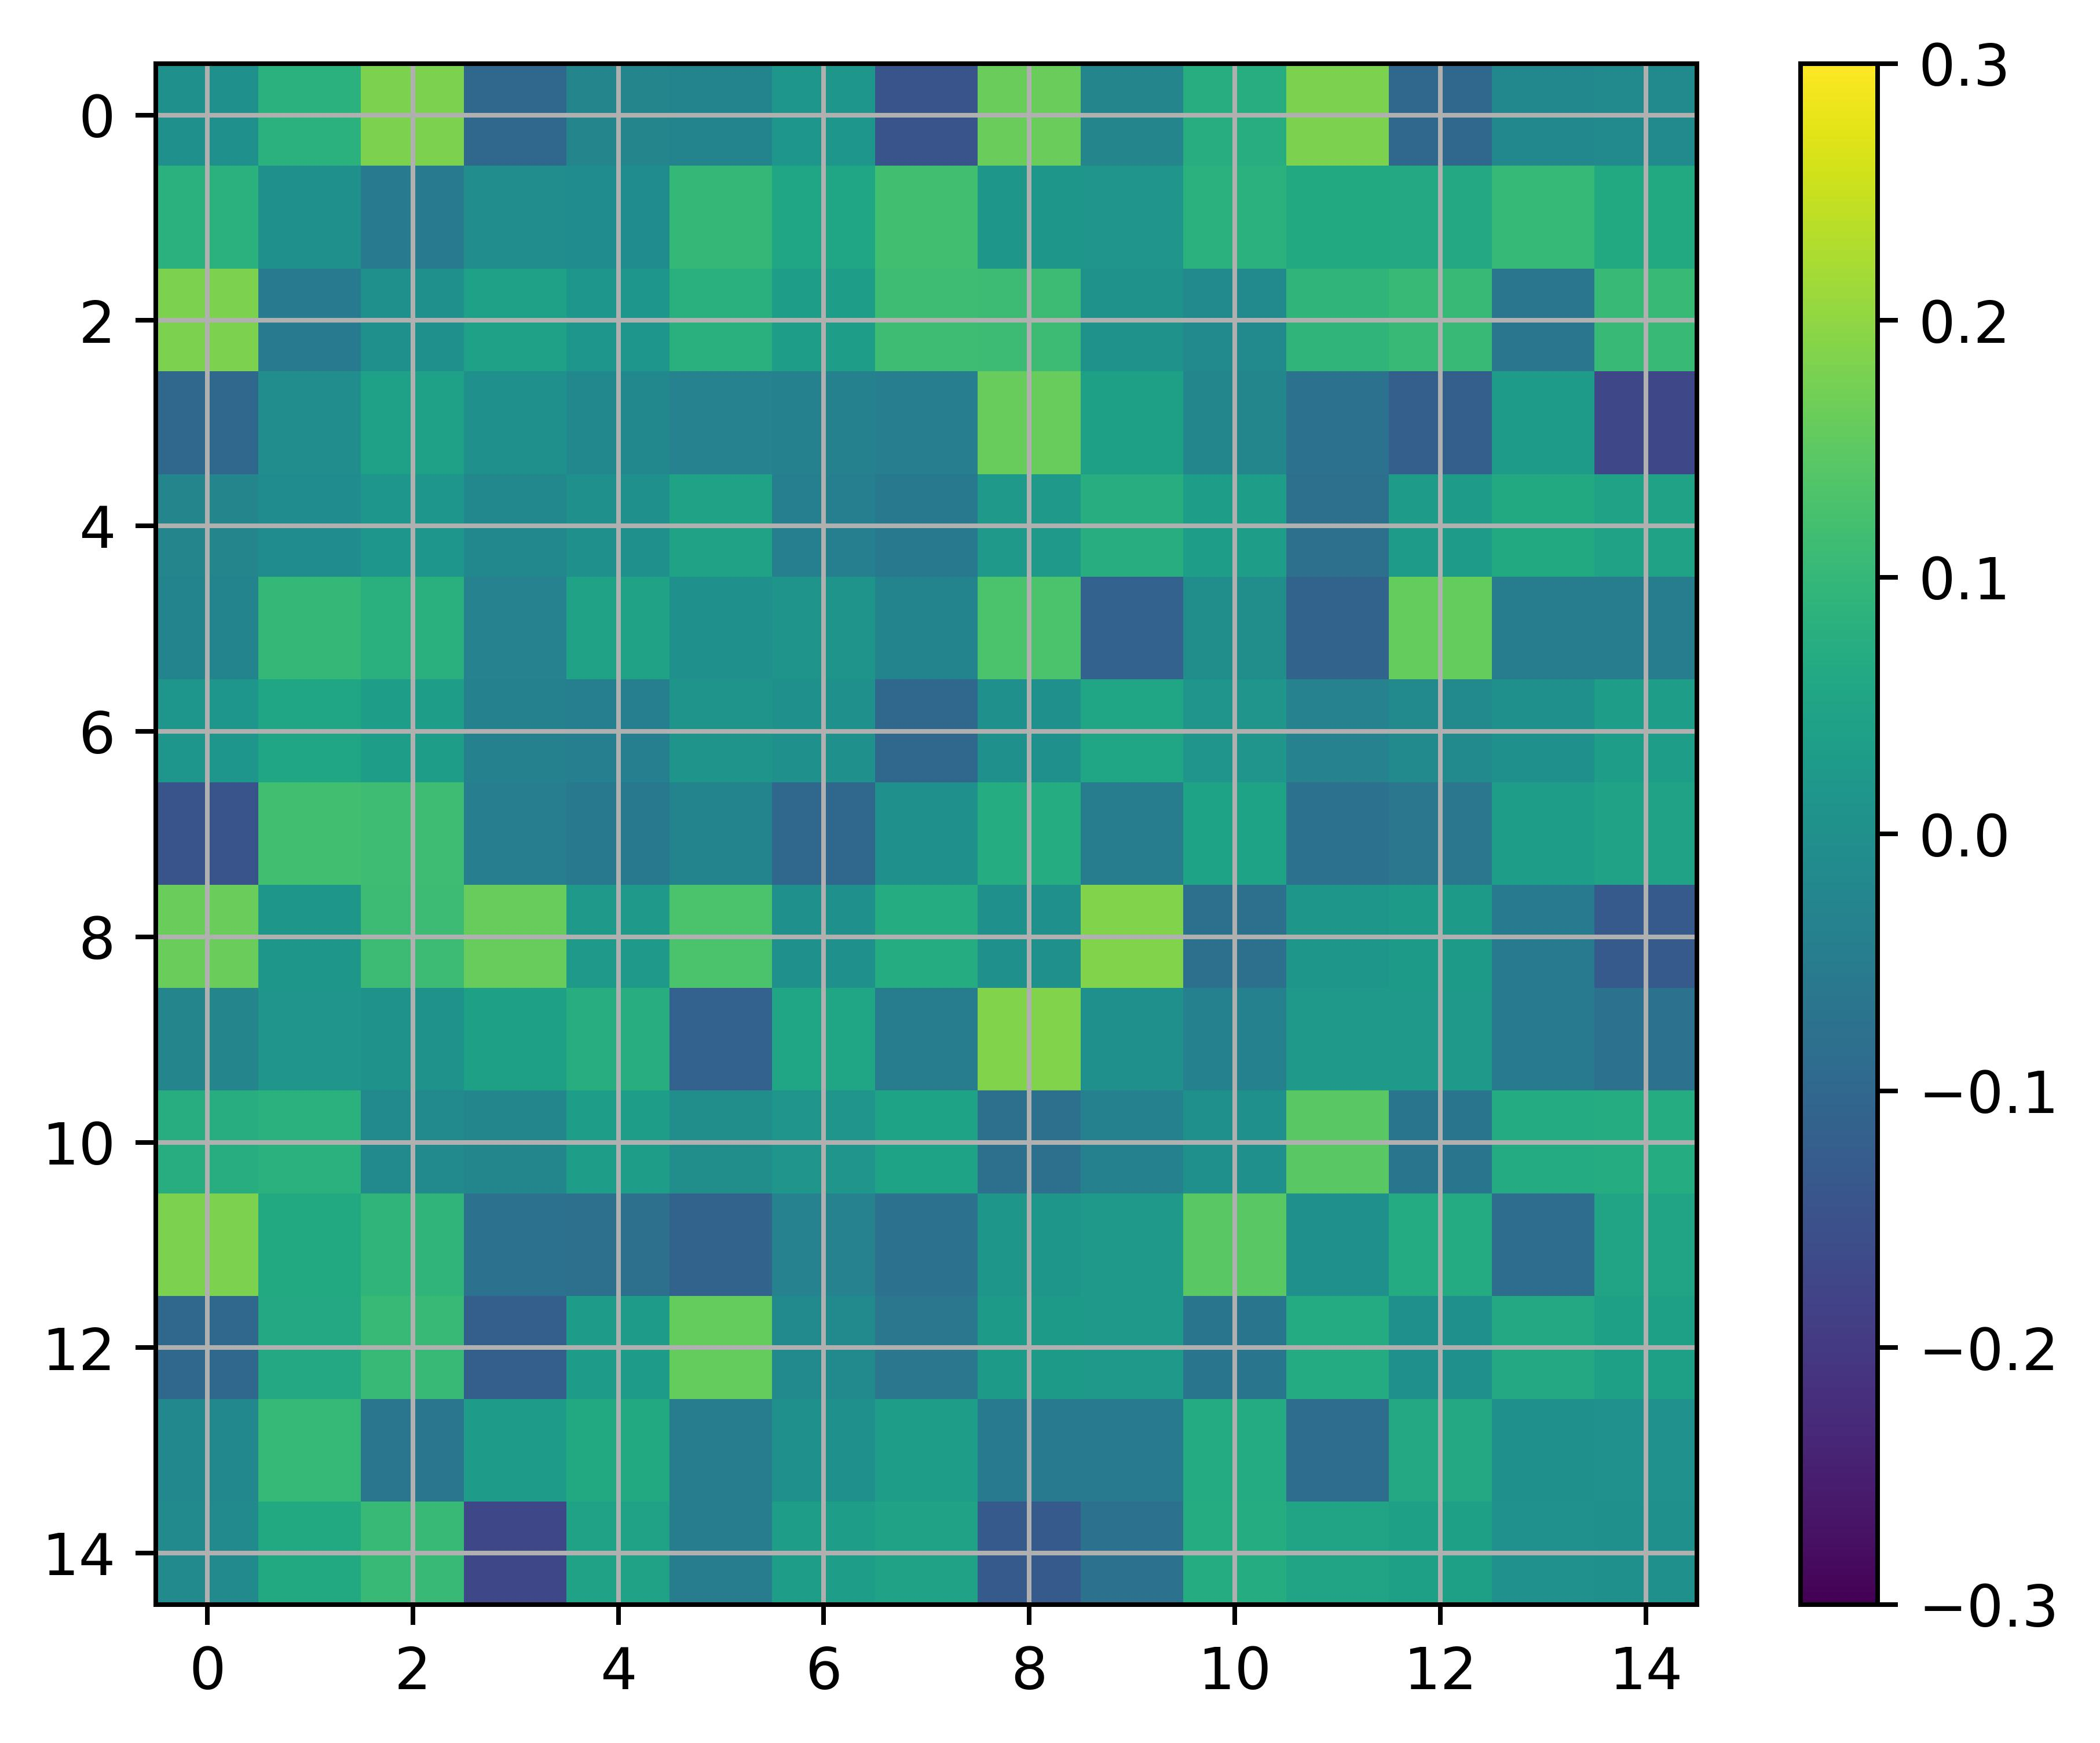
\includegraphics[width=0.2\textwidth]{../Analysis/DFC/size=480_step=180_rho=0.1/node=15_id=100206/c_18.jpg}
        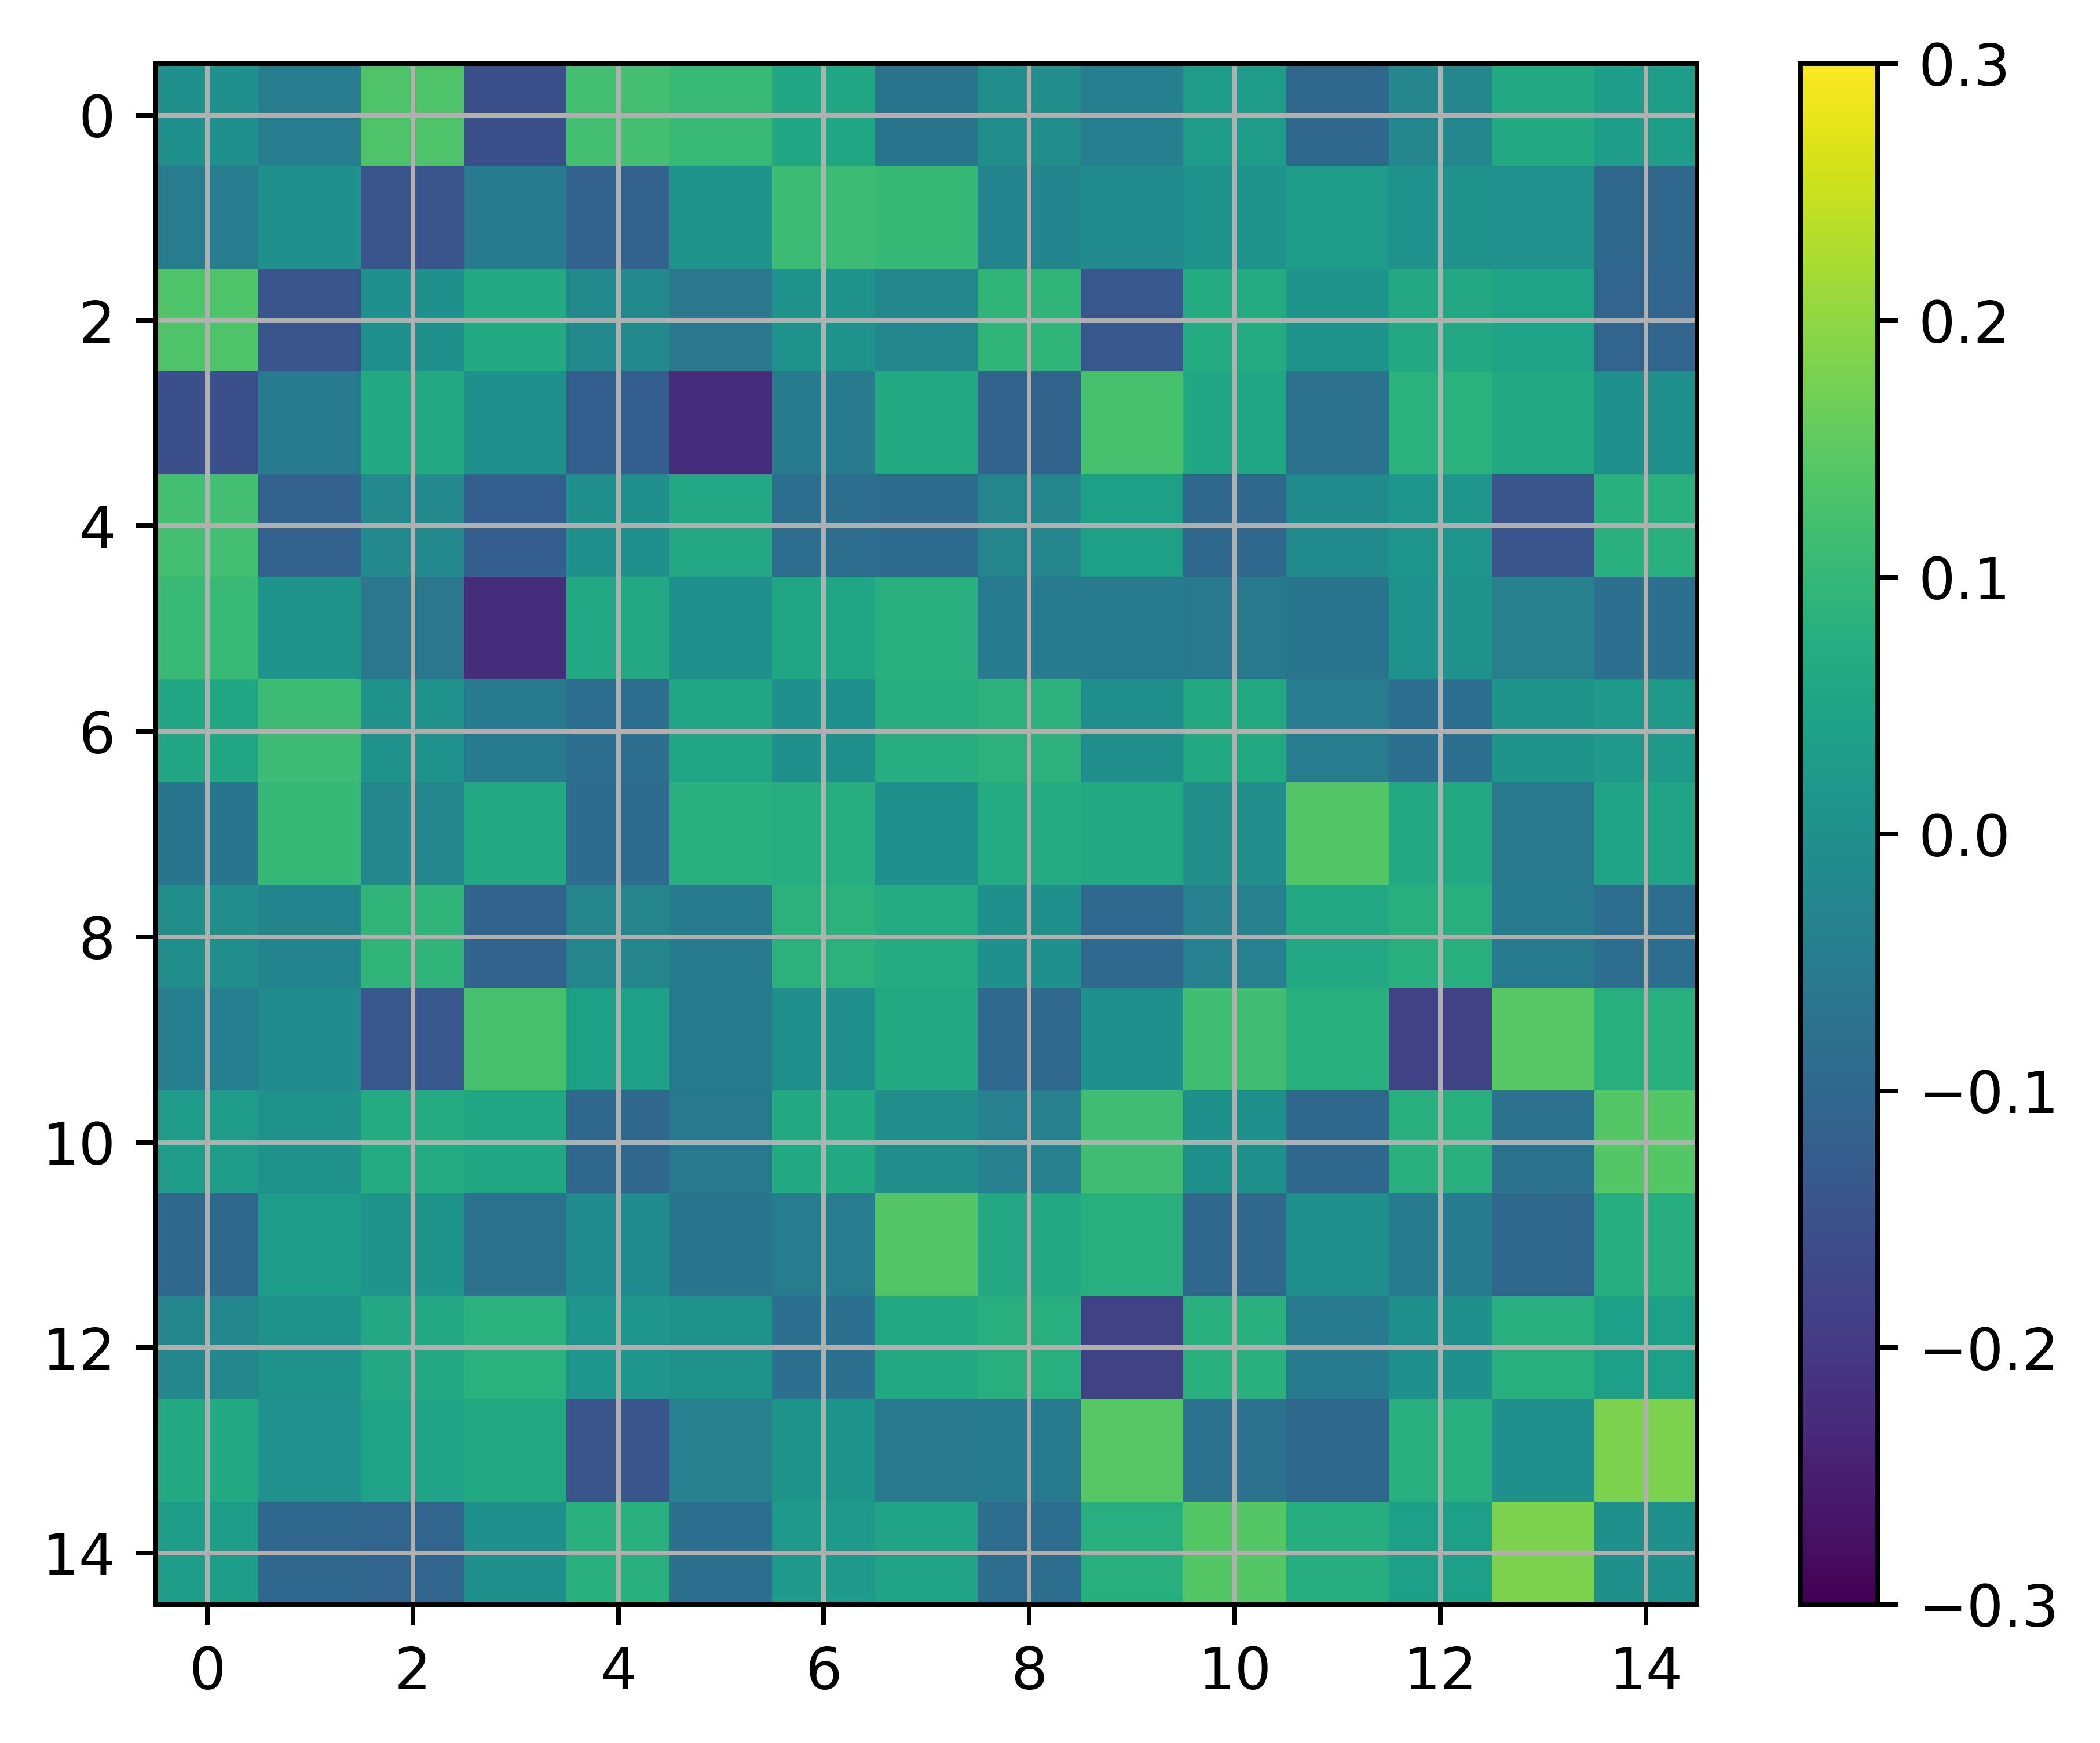
\includegraphics[width=0.2\textwidth]{../Analysis/DFC/size=480_step=180_rho=0.1/node=15_id=100206/c_20.jpg}
        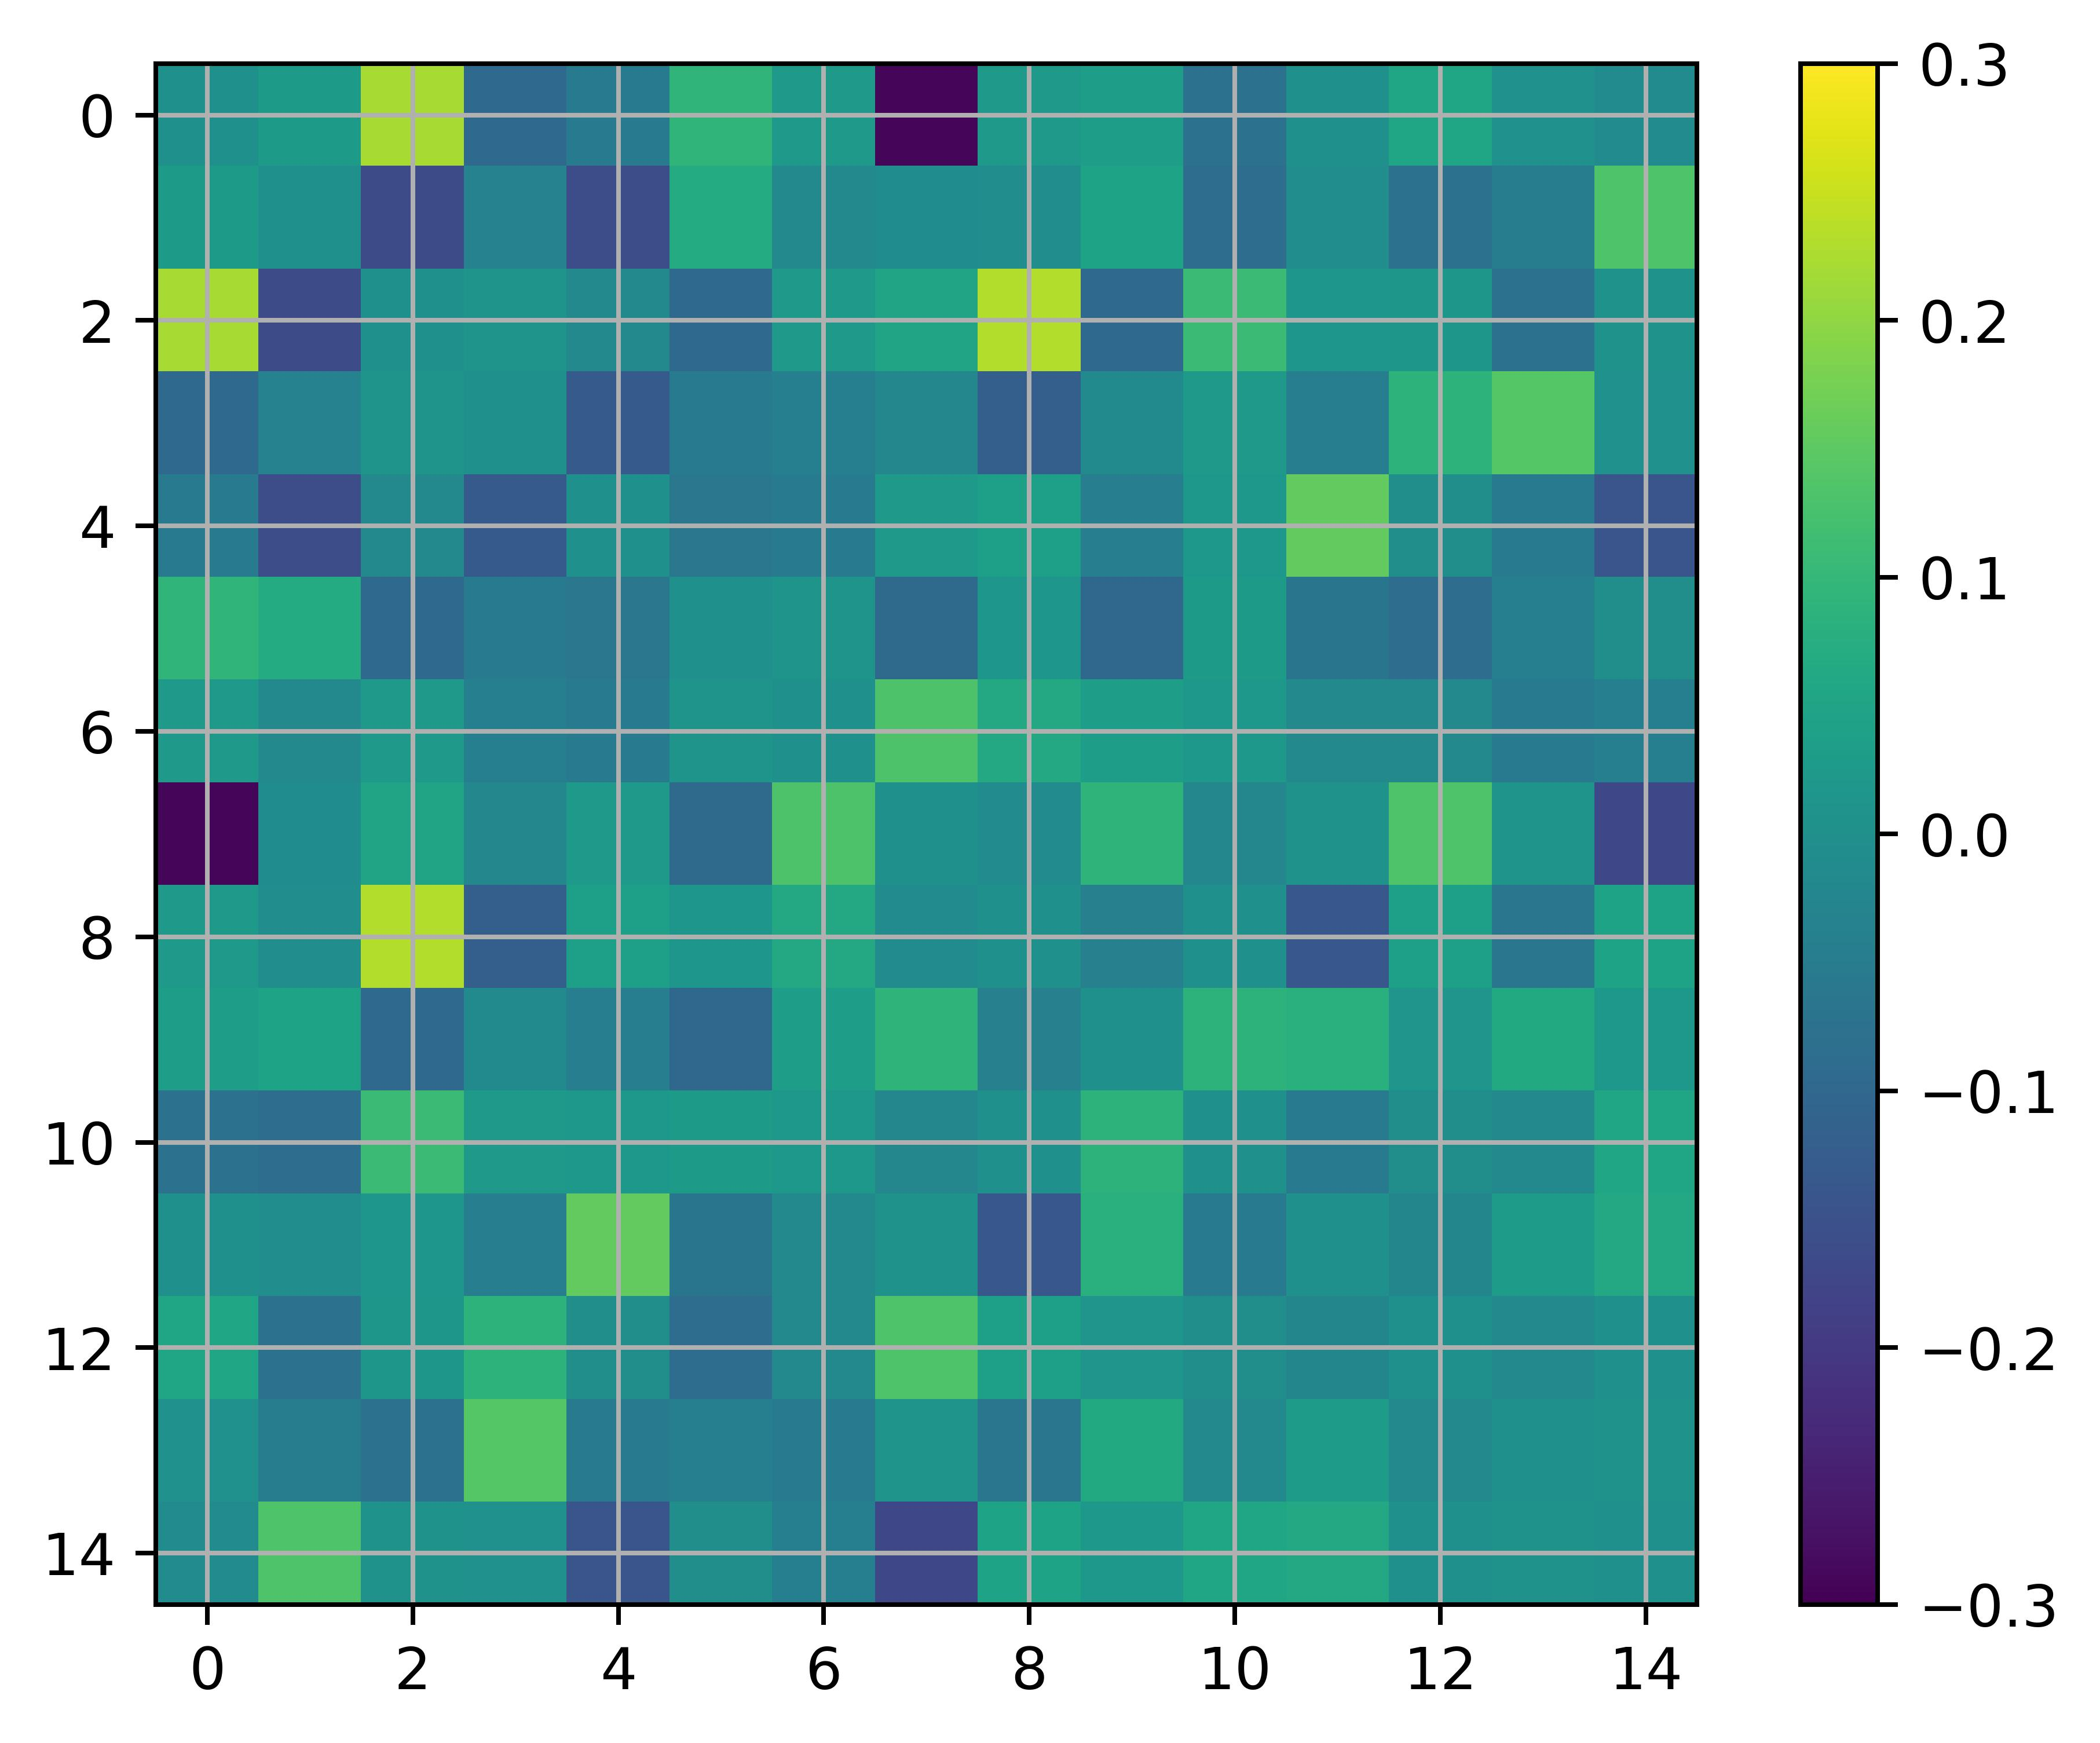
\includegraphics[width=0.2\textwidth]{../Analysis/DFC/size=480_step=180_rho=0.1/node=15_id=100206/c_22.jpg} \\
        \caption{Centered dynamic functional connectivity with $N_{node} = 15$.}
        % \label{LDA-example-1}
    \end{figure}

\end{frame}

\begin{frame}{Preprocessing - Examples}

    \begin{figure}[H]
        \centering
        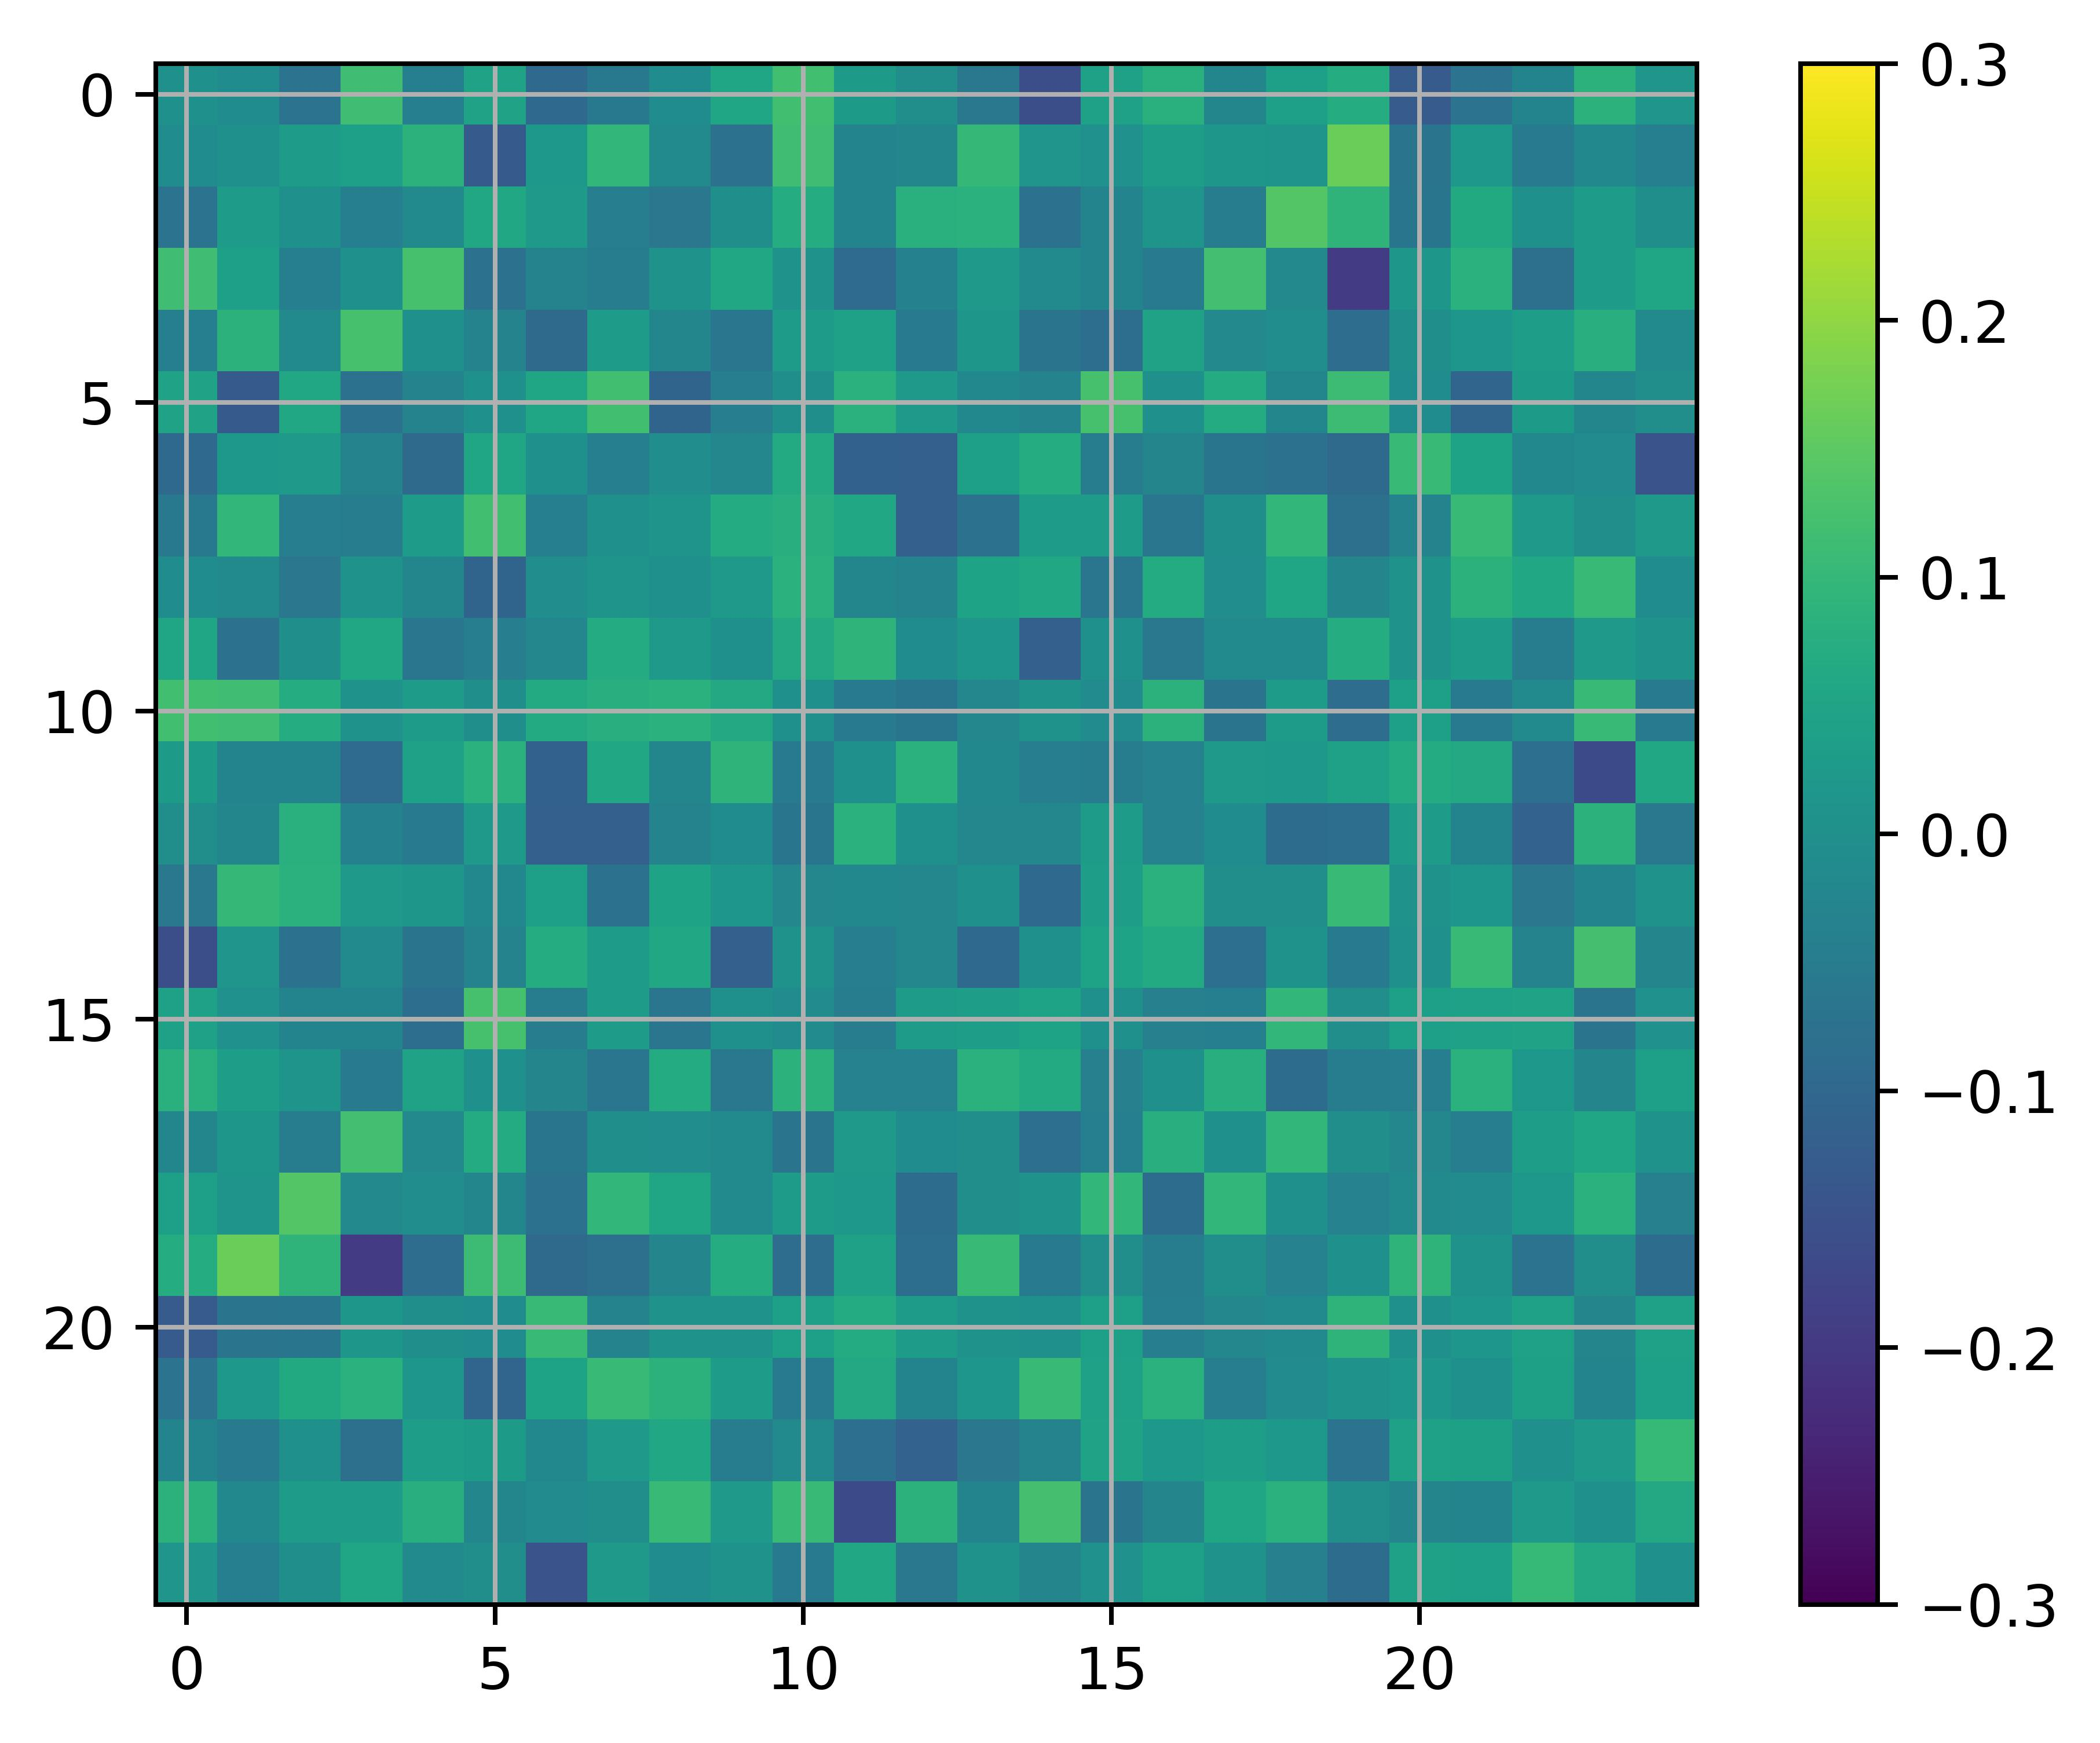
\includegraphics[width=0.2\textwidth]{../Analysis/DFC/size=480_step=180_rho=0.1/node=25_id=100206/c_0.jpg}
        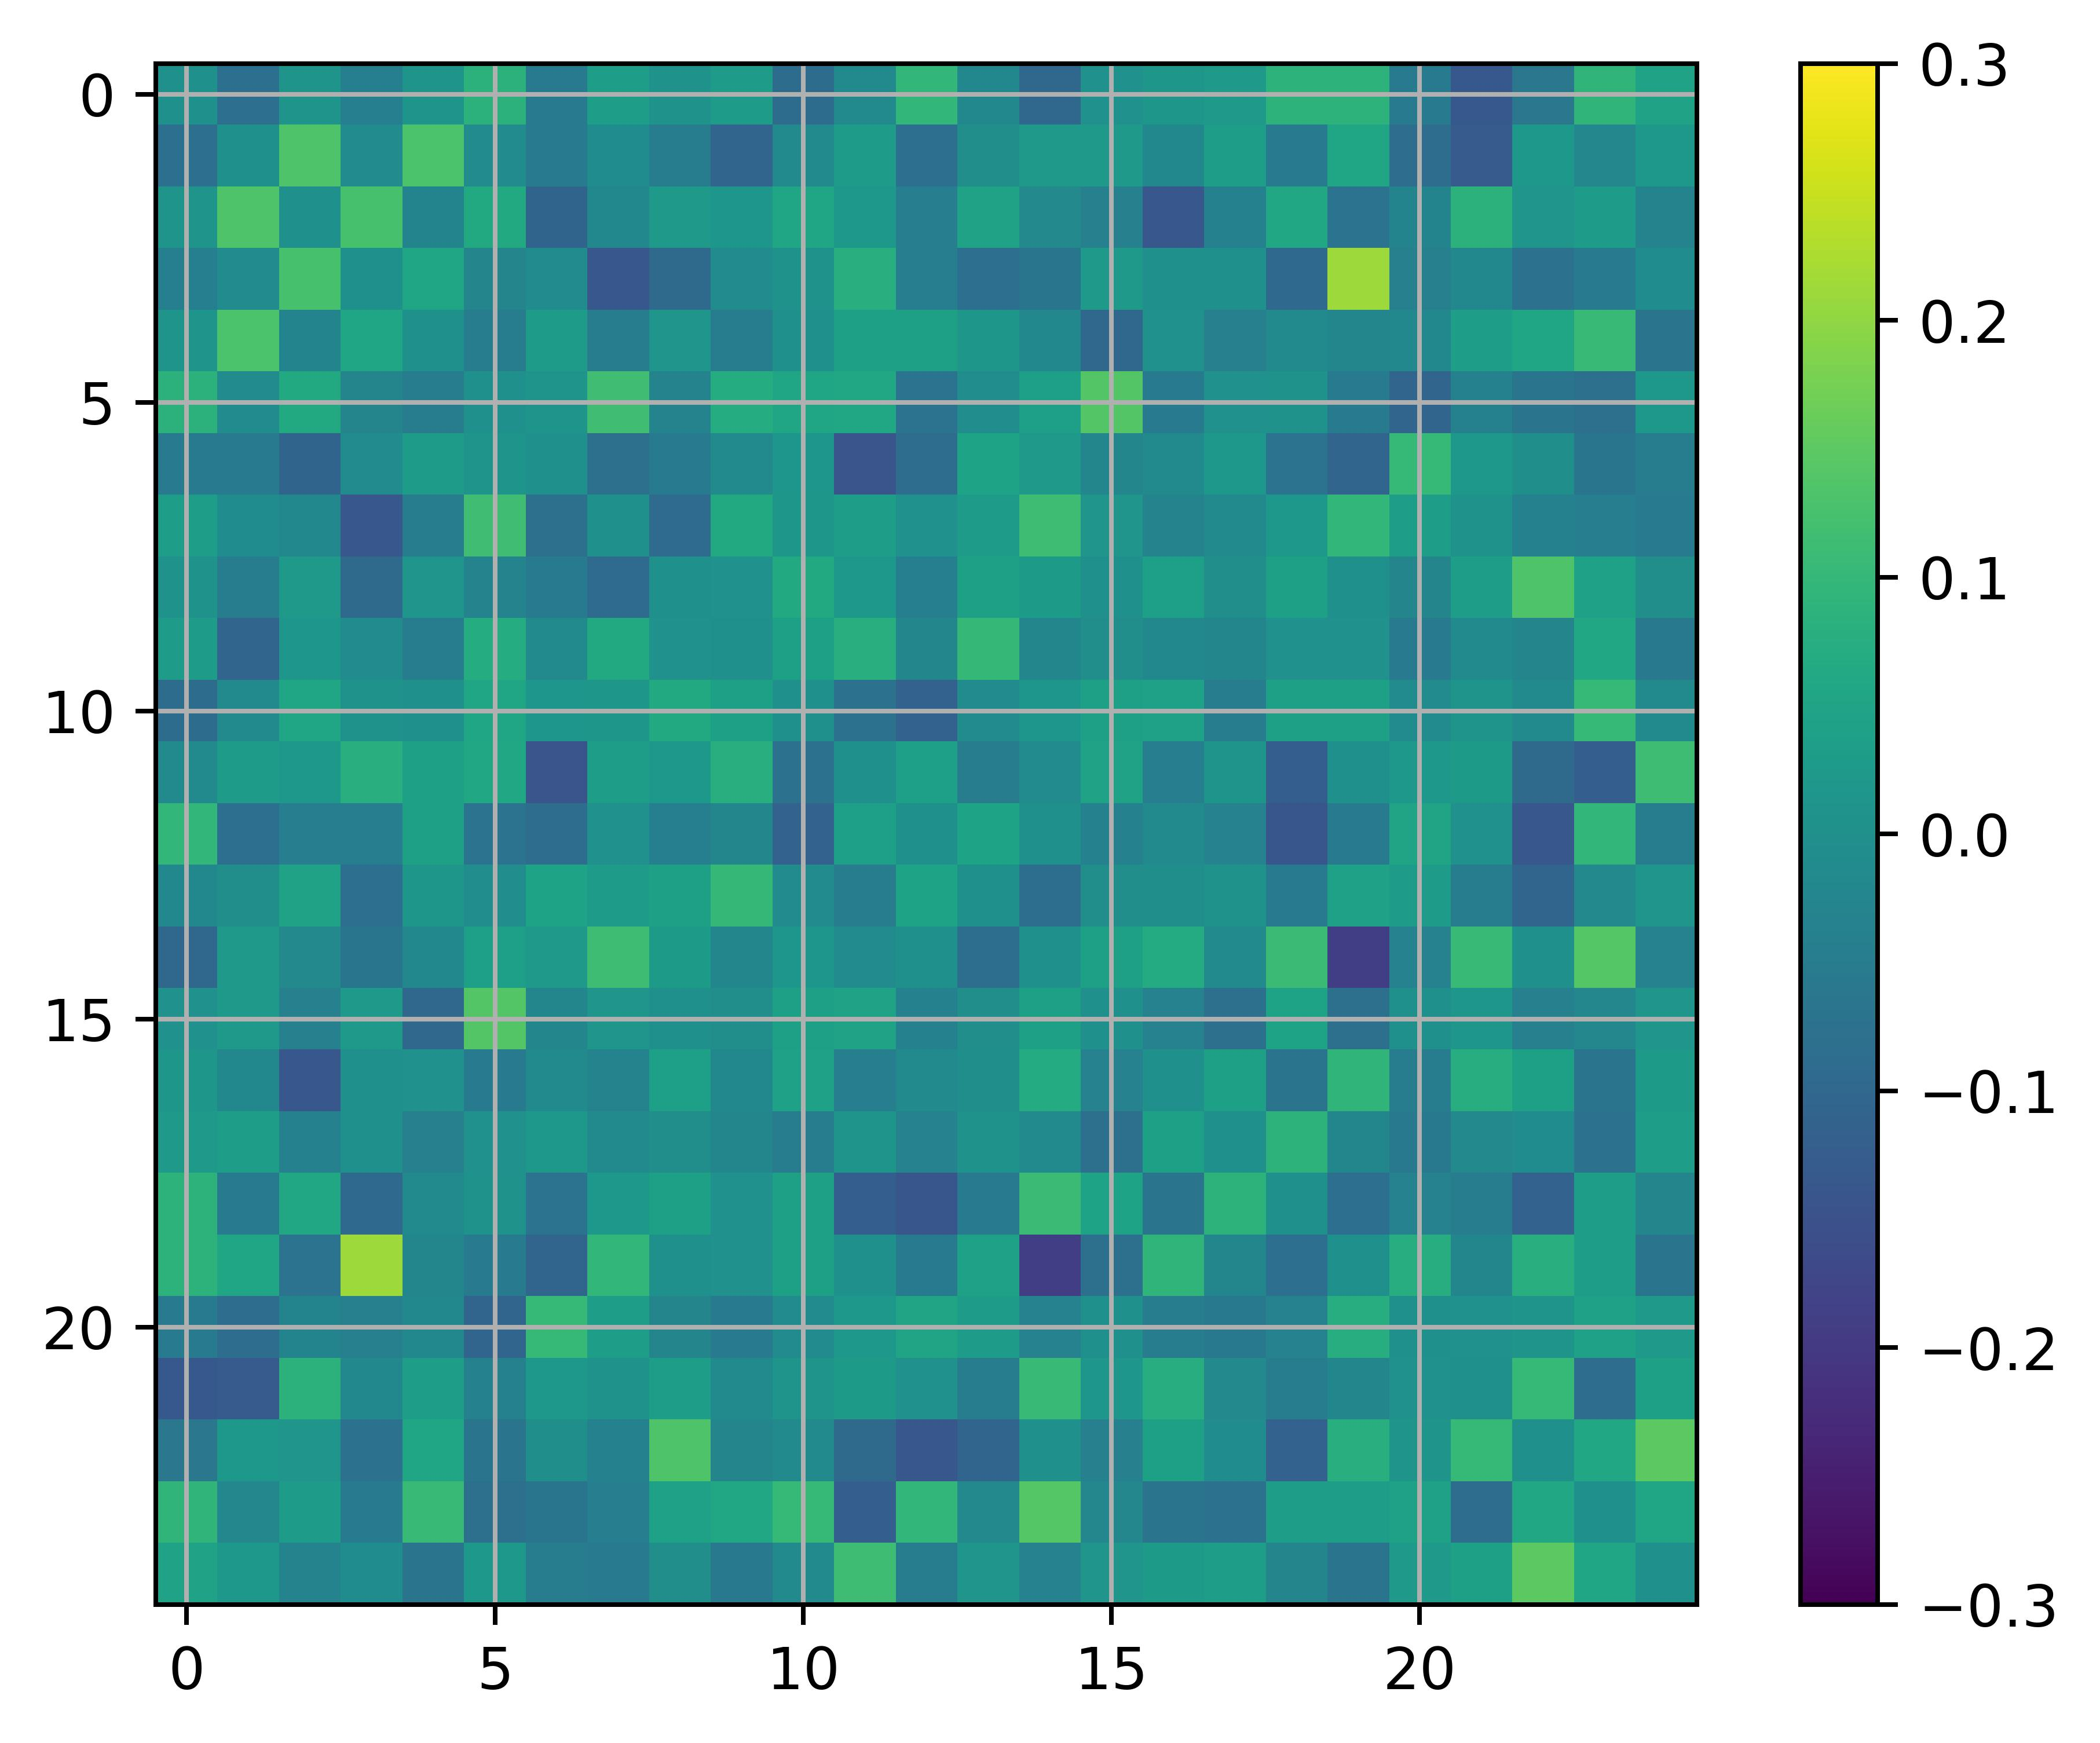
\includegraphics[width=0.2\textwidth]{../Analysis/DFC/size=480_step=180_rho=0.1/node=25_id=100206/c_2.jpg}
        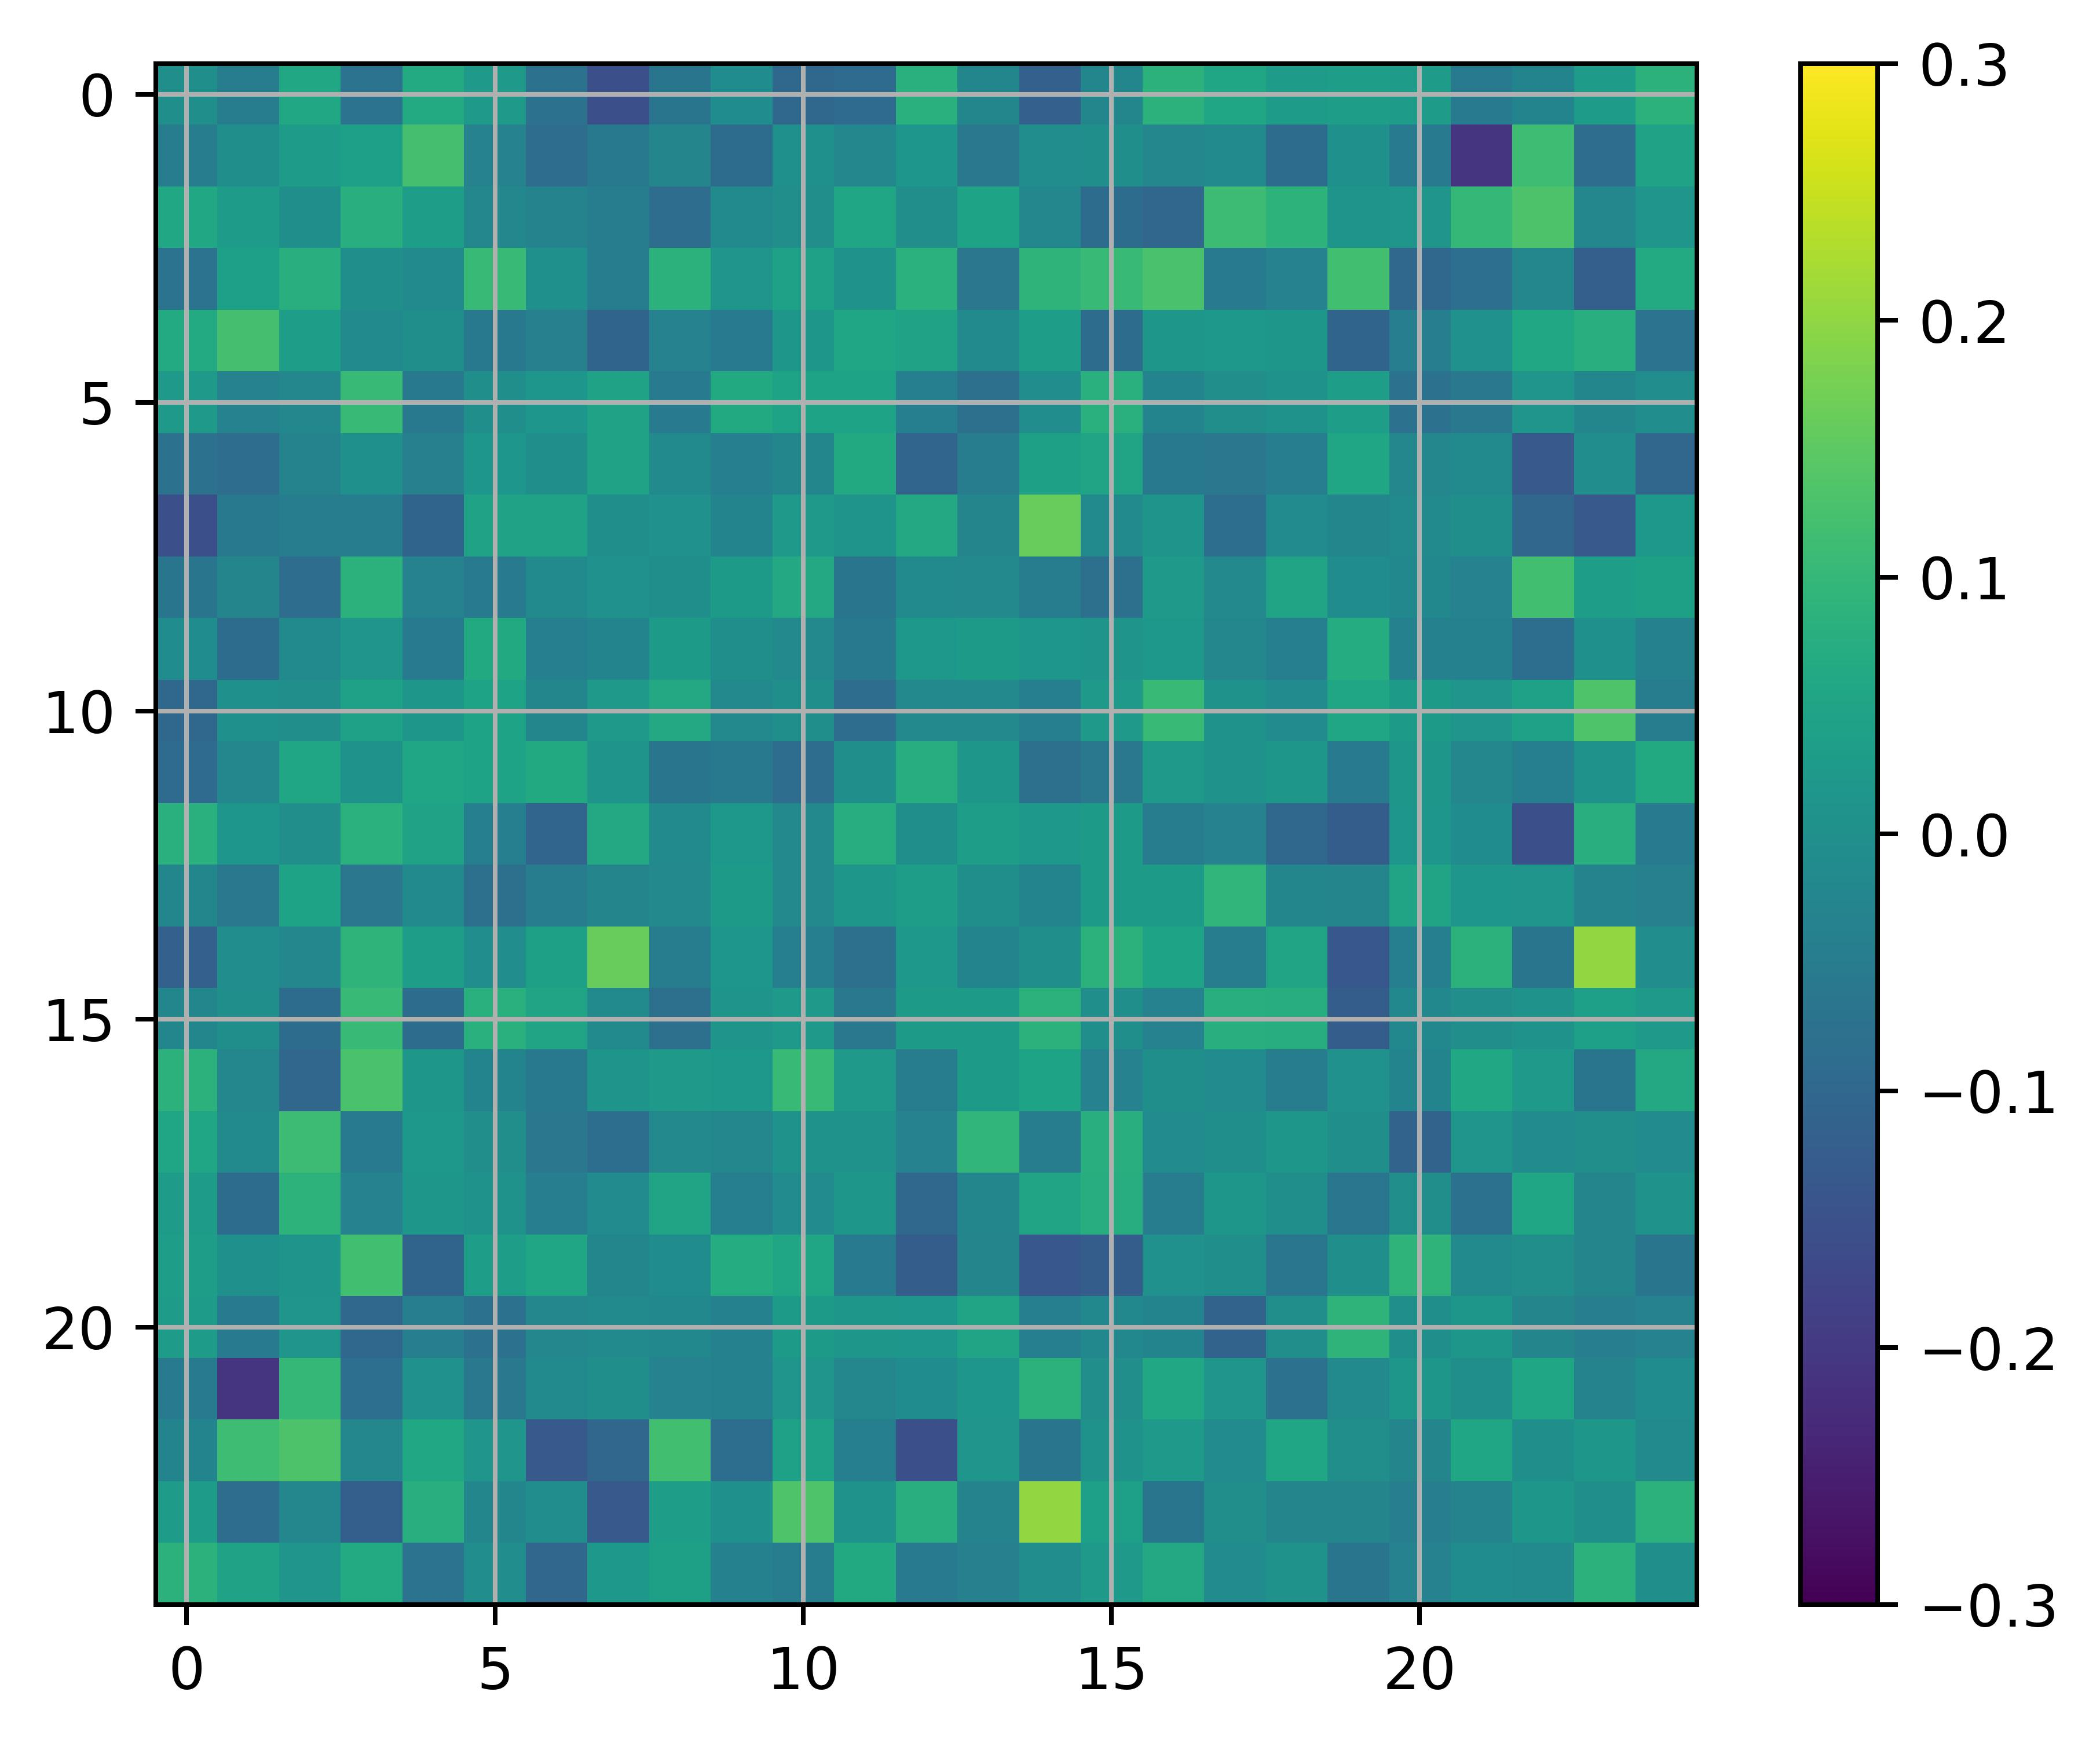
\includegraphics[width=0.2\textwidth]{../Analysis/DFC/size=480_step=180_rho=0.1/node=25_id=100206/c_4.jpg}
        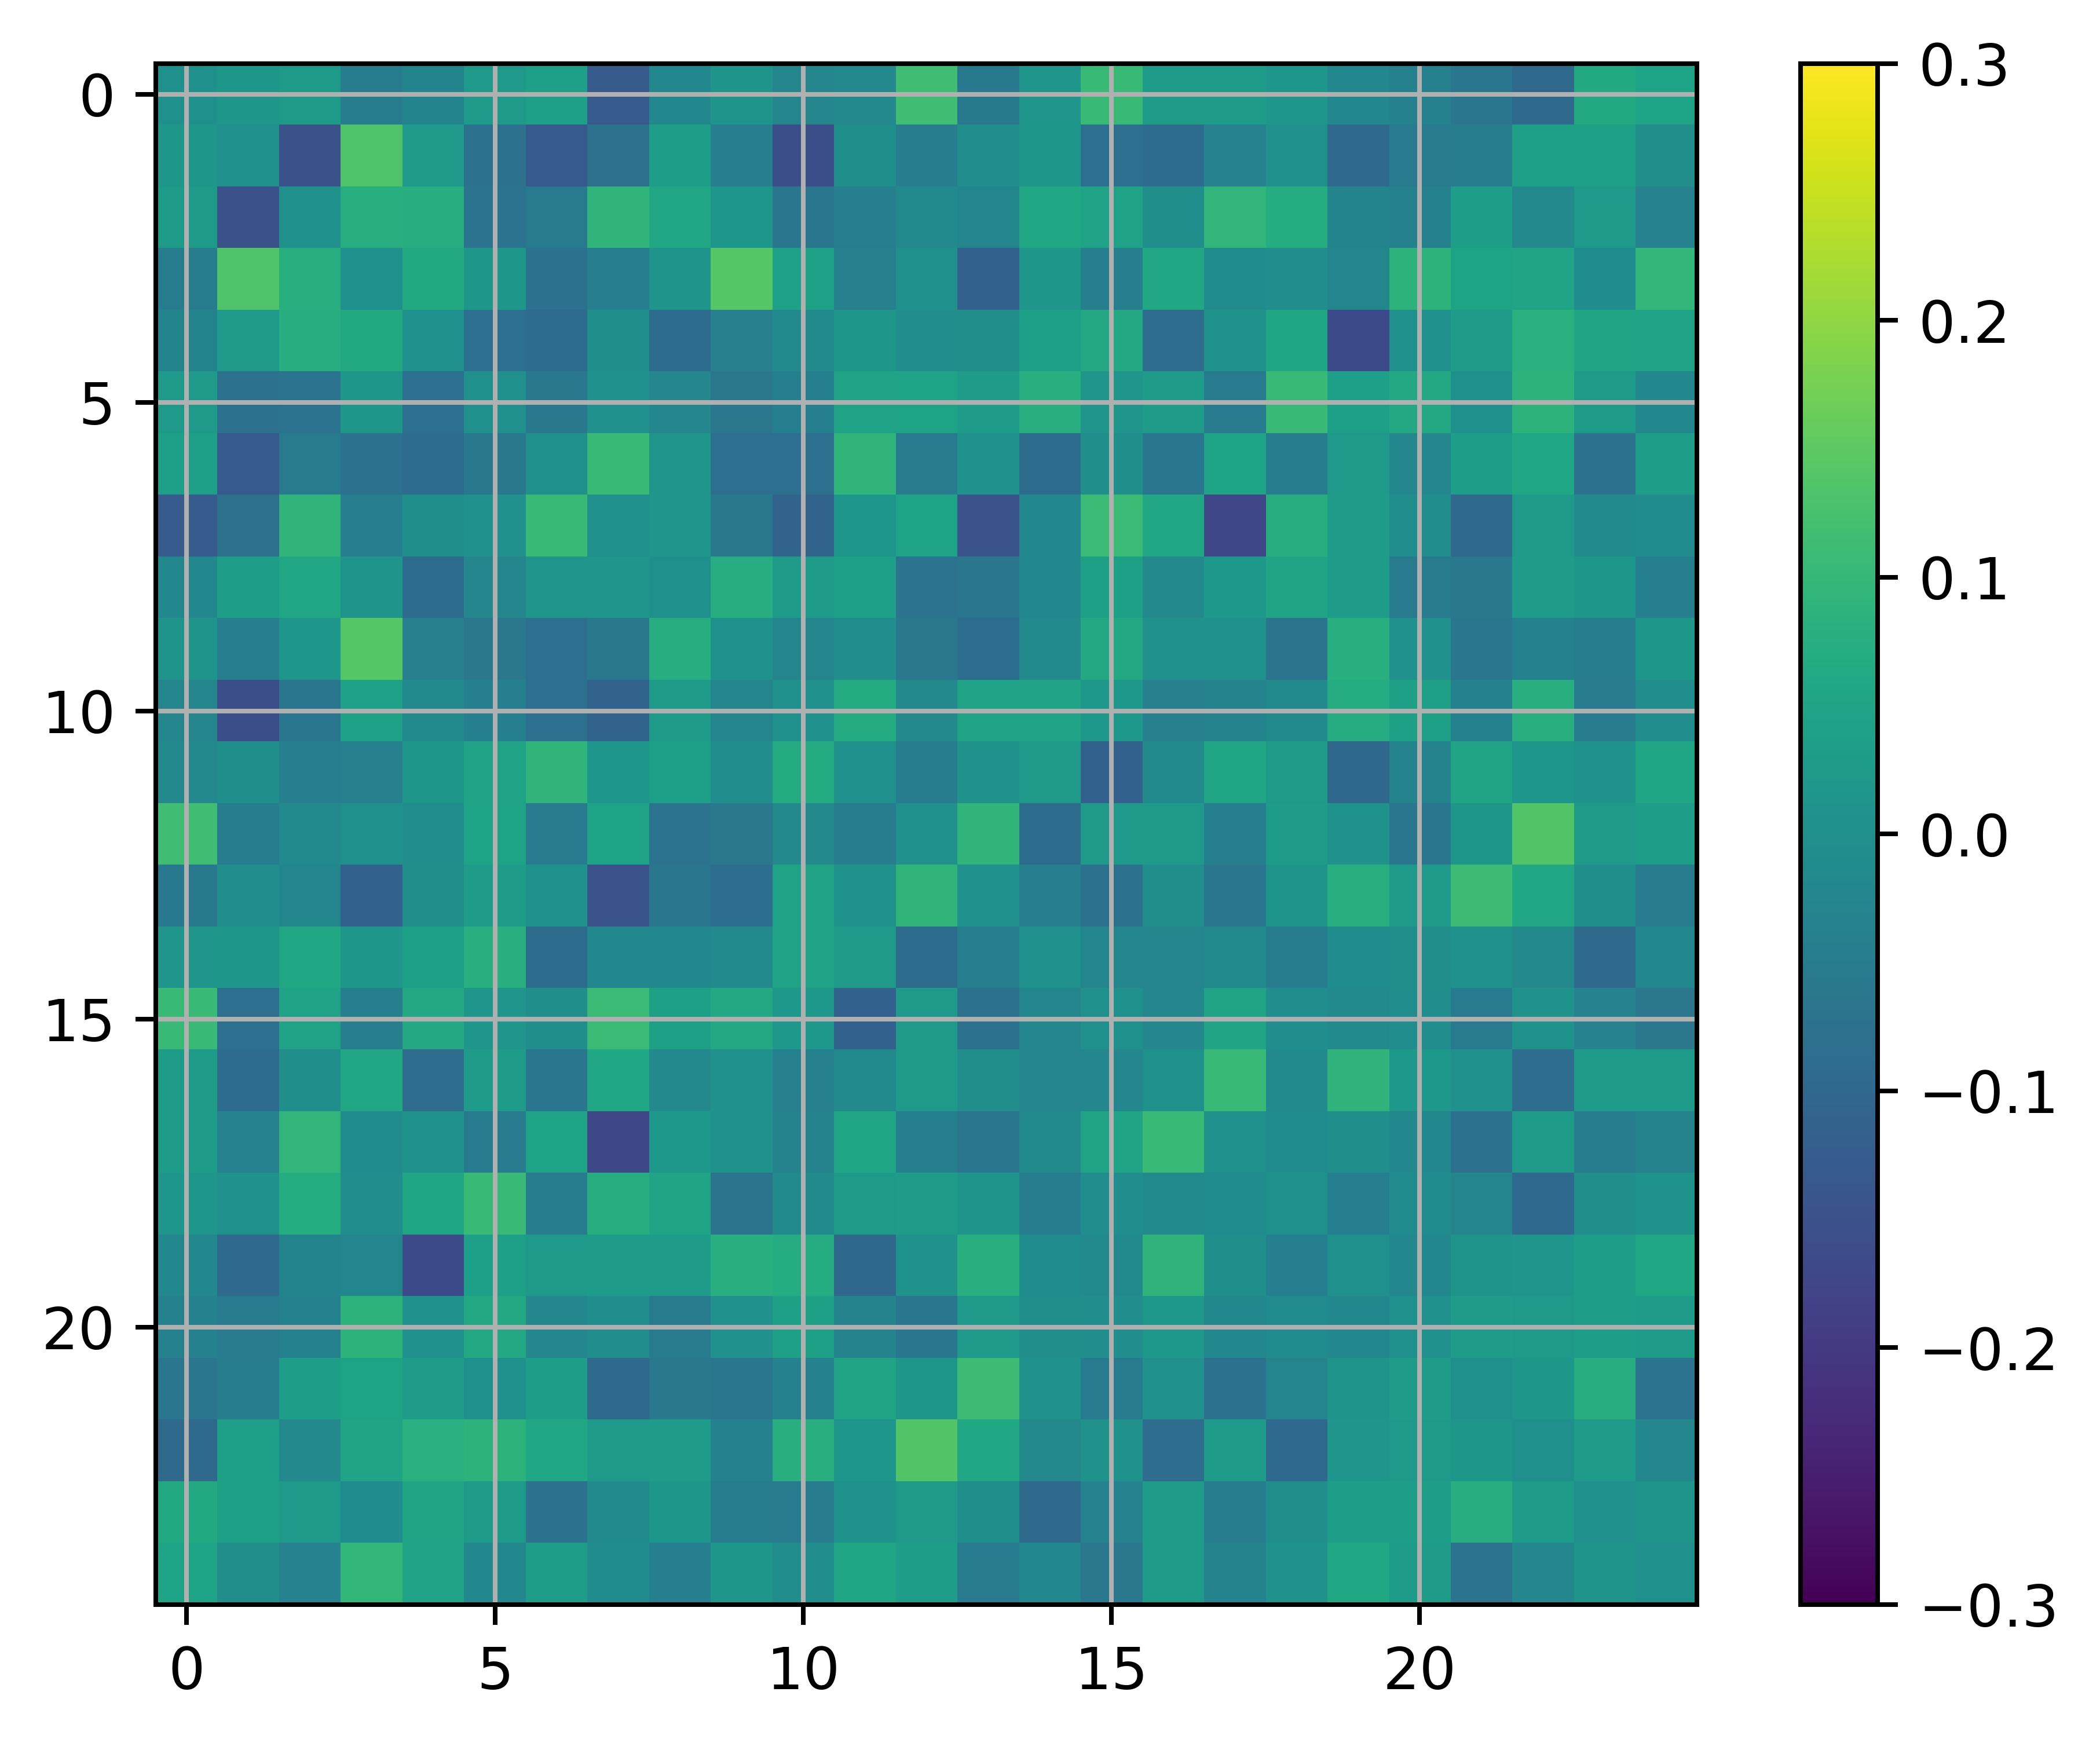
\includegraphics[width=0.2\textwidth]{../Analysis/DFC/size=480_step=180_rho=0.1/node=25_id=100206/c_6.jpg} \\
        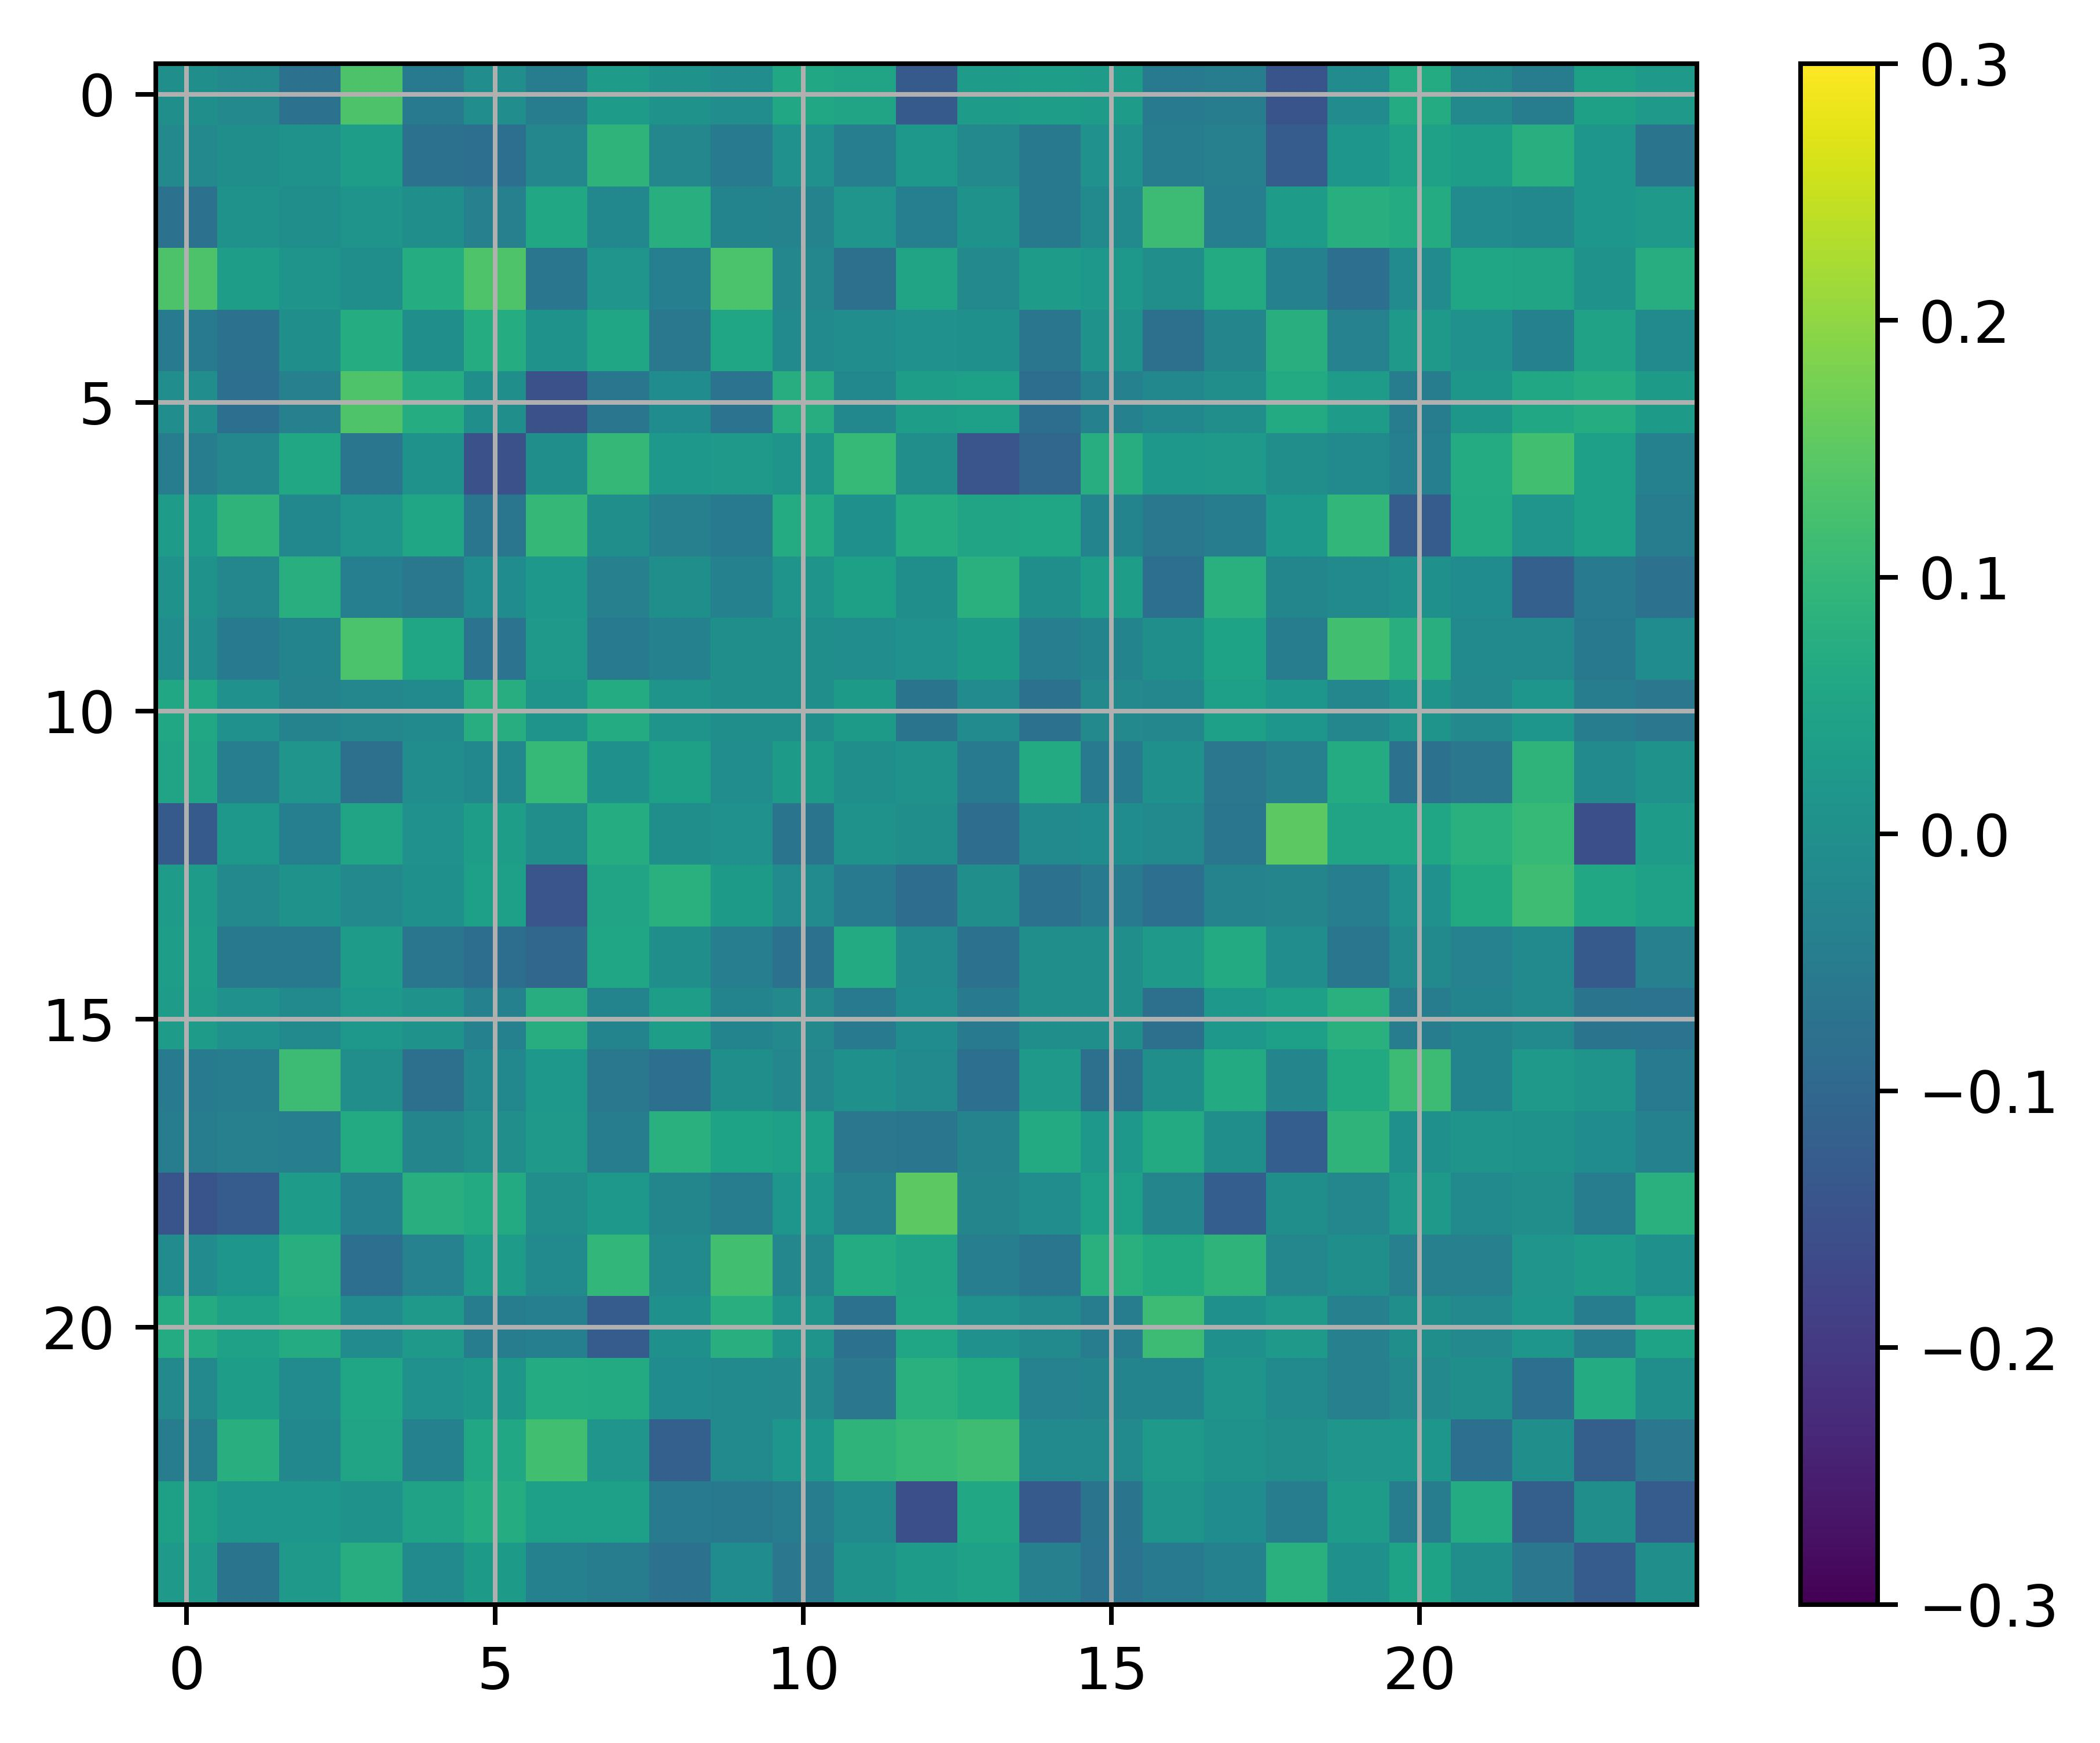
\includegraphics[width=0.2\textwidth]{../Analysis/DFC/size=480_step=180_rho=0.1/node=25_id=100206/c_8.jpg}
        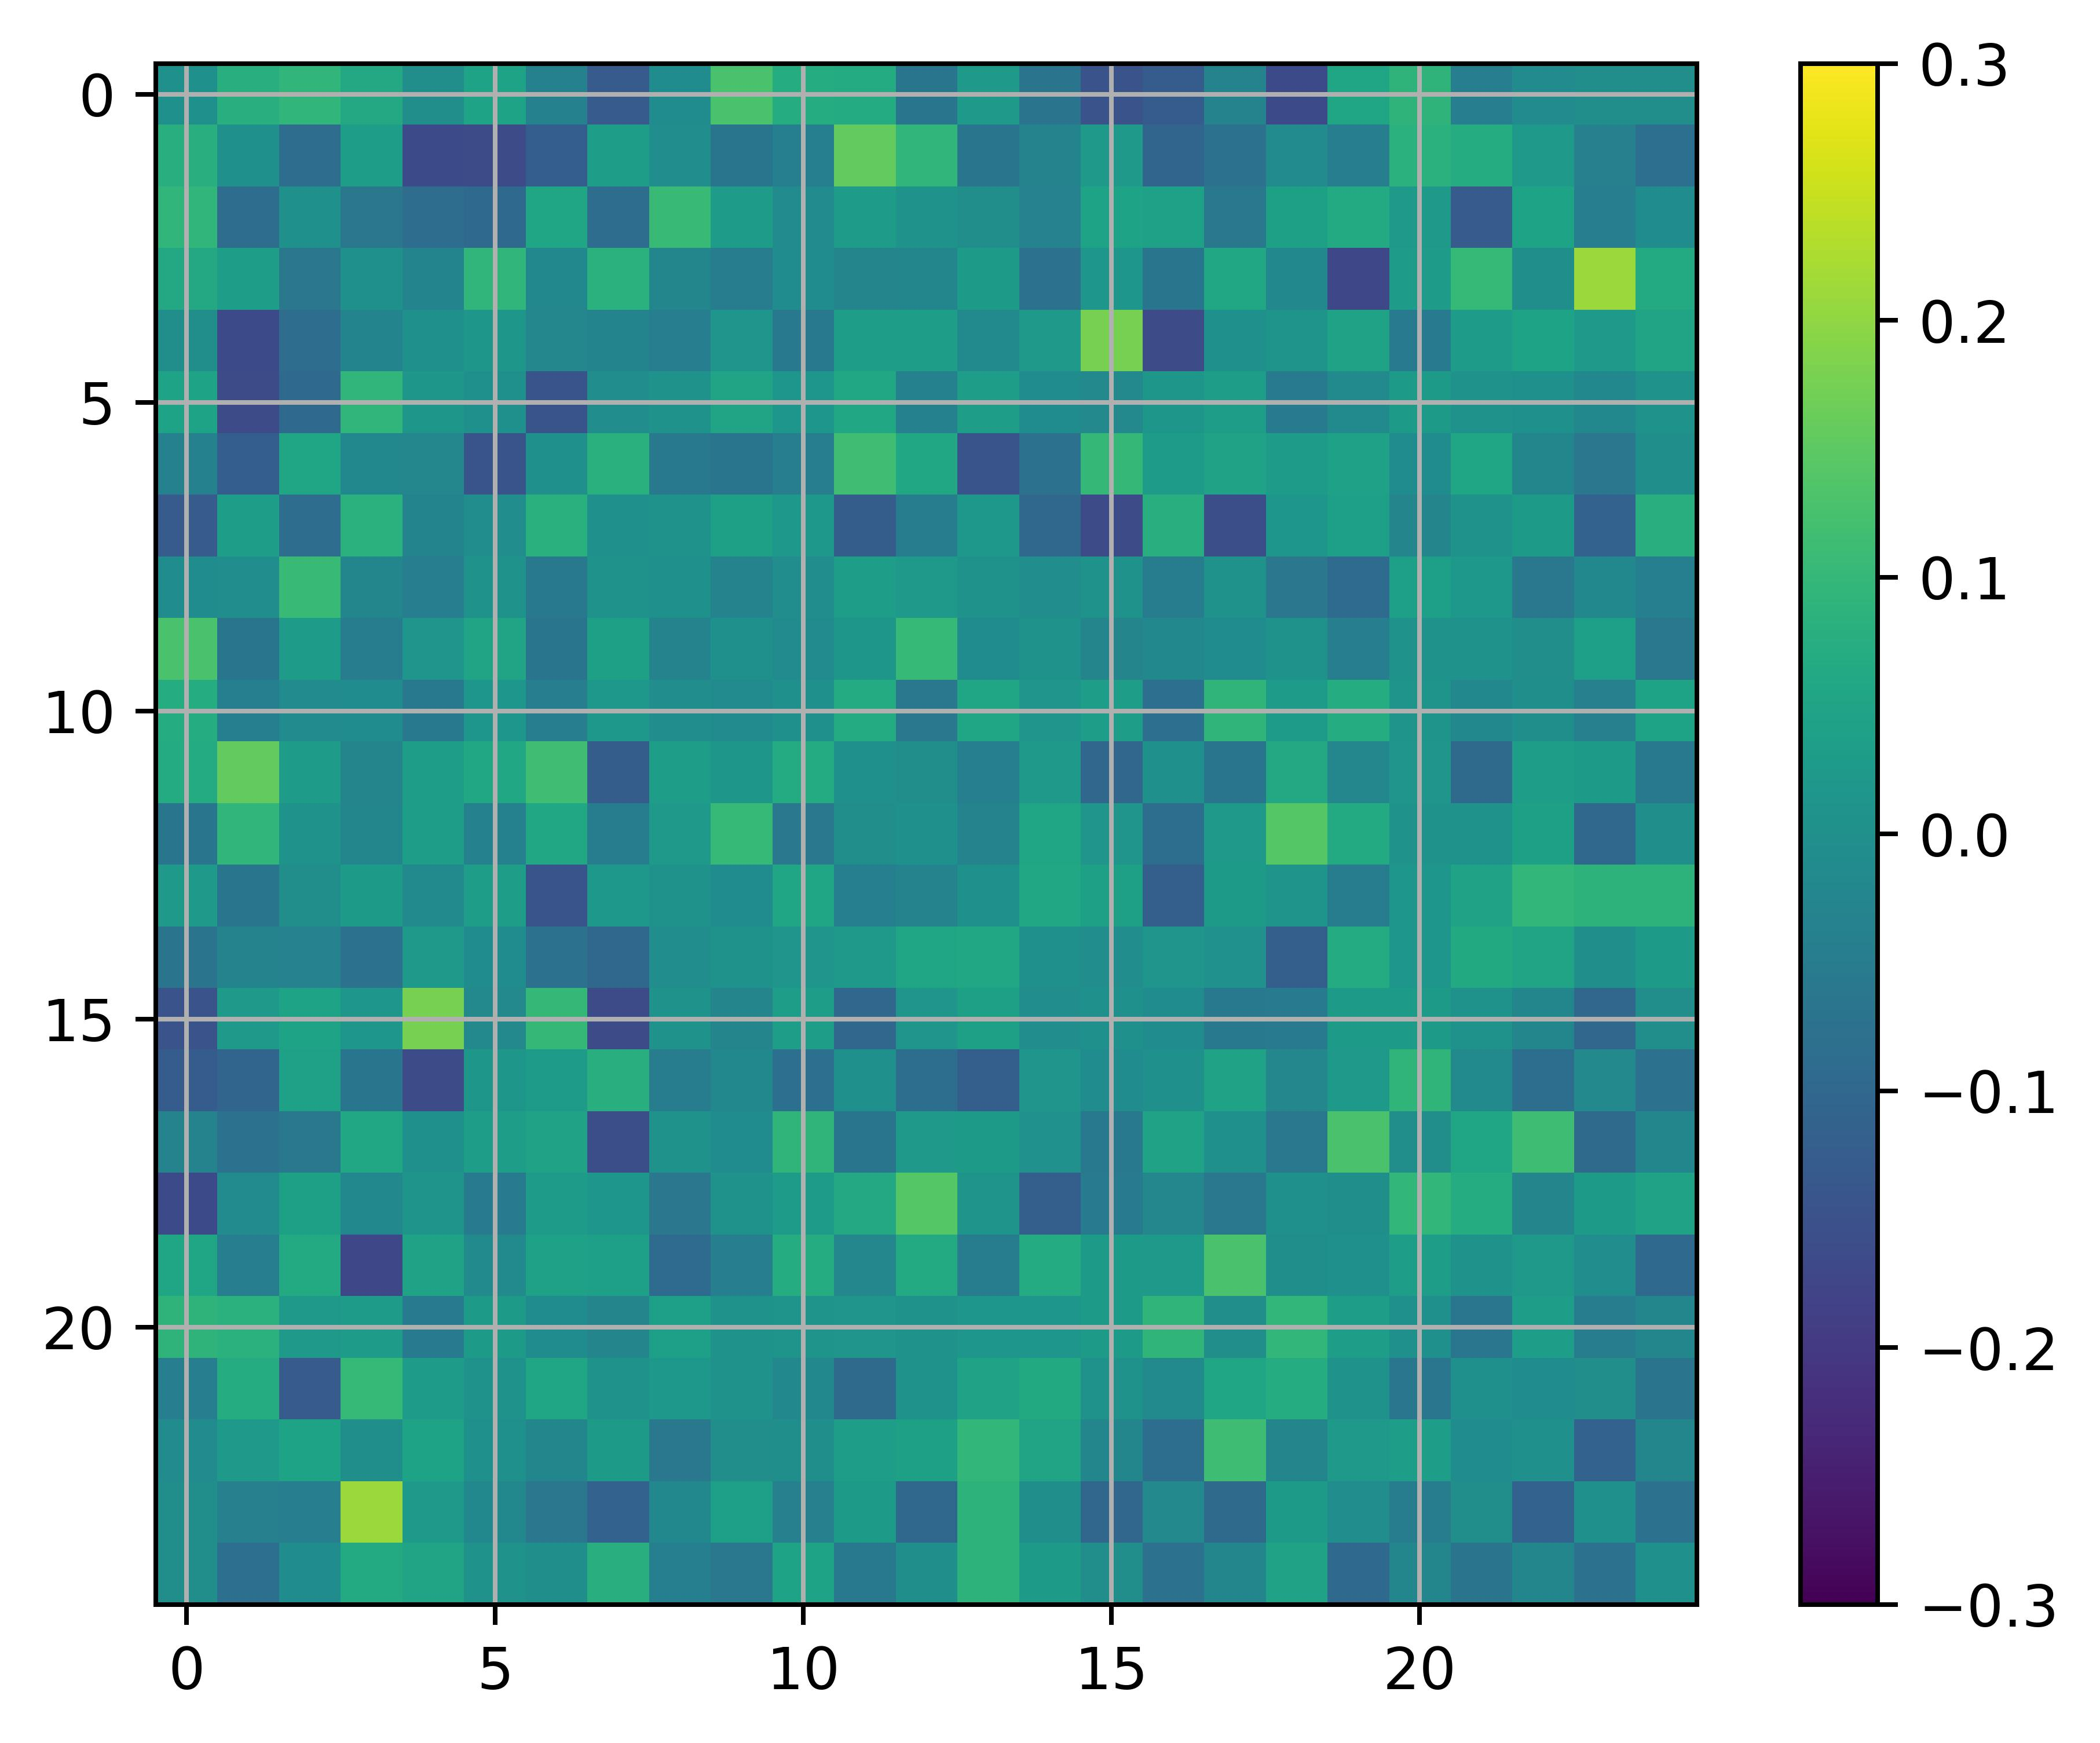
\includegraphics[width=0.2\textwidth]{../Analysis/DFC/size=480_step=180_rho=0.1/node=25_id=100206/c_10.jpg}
        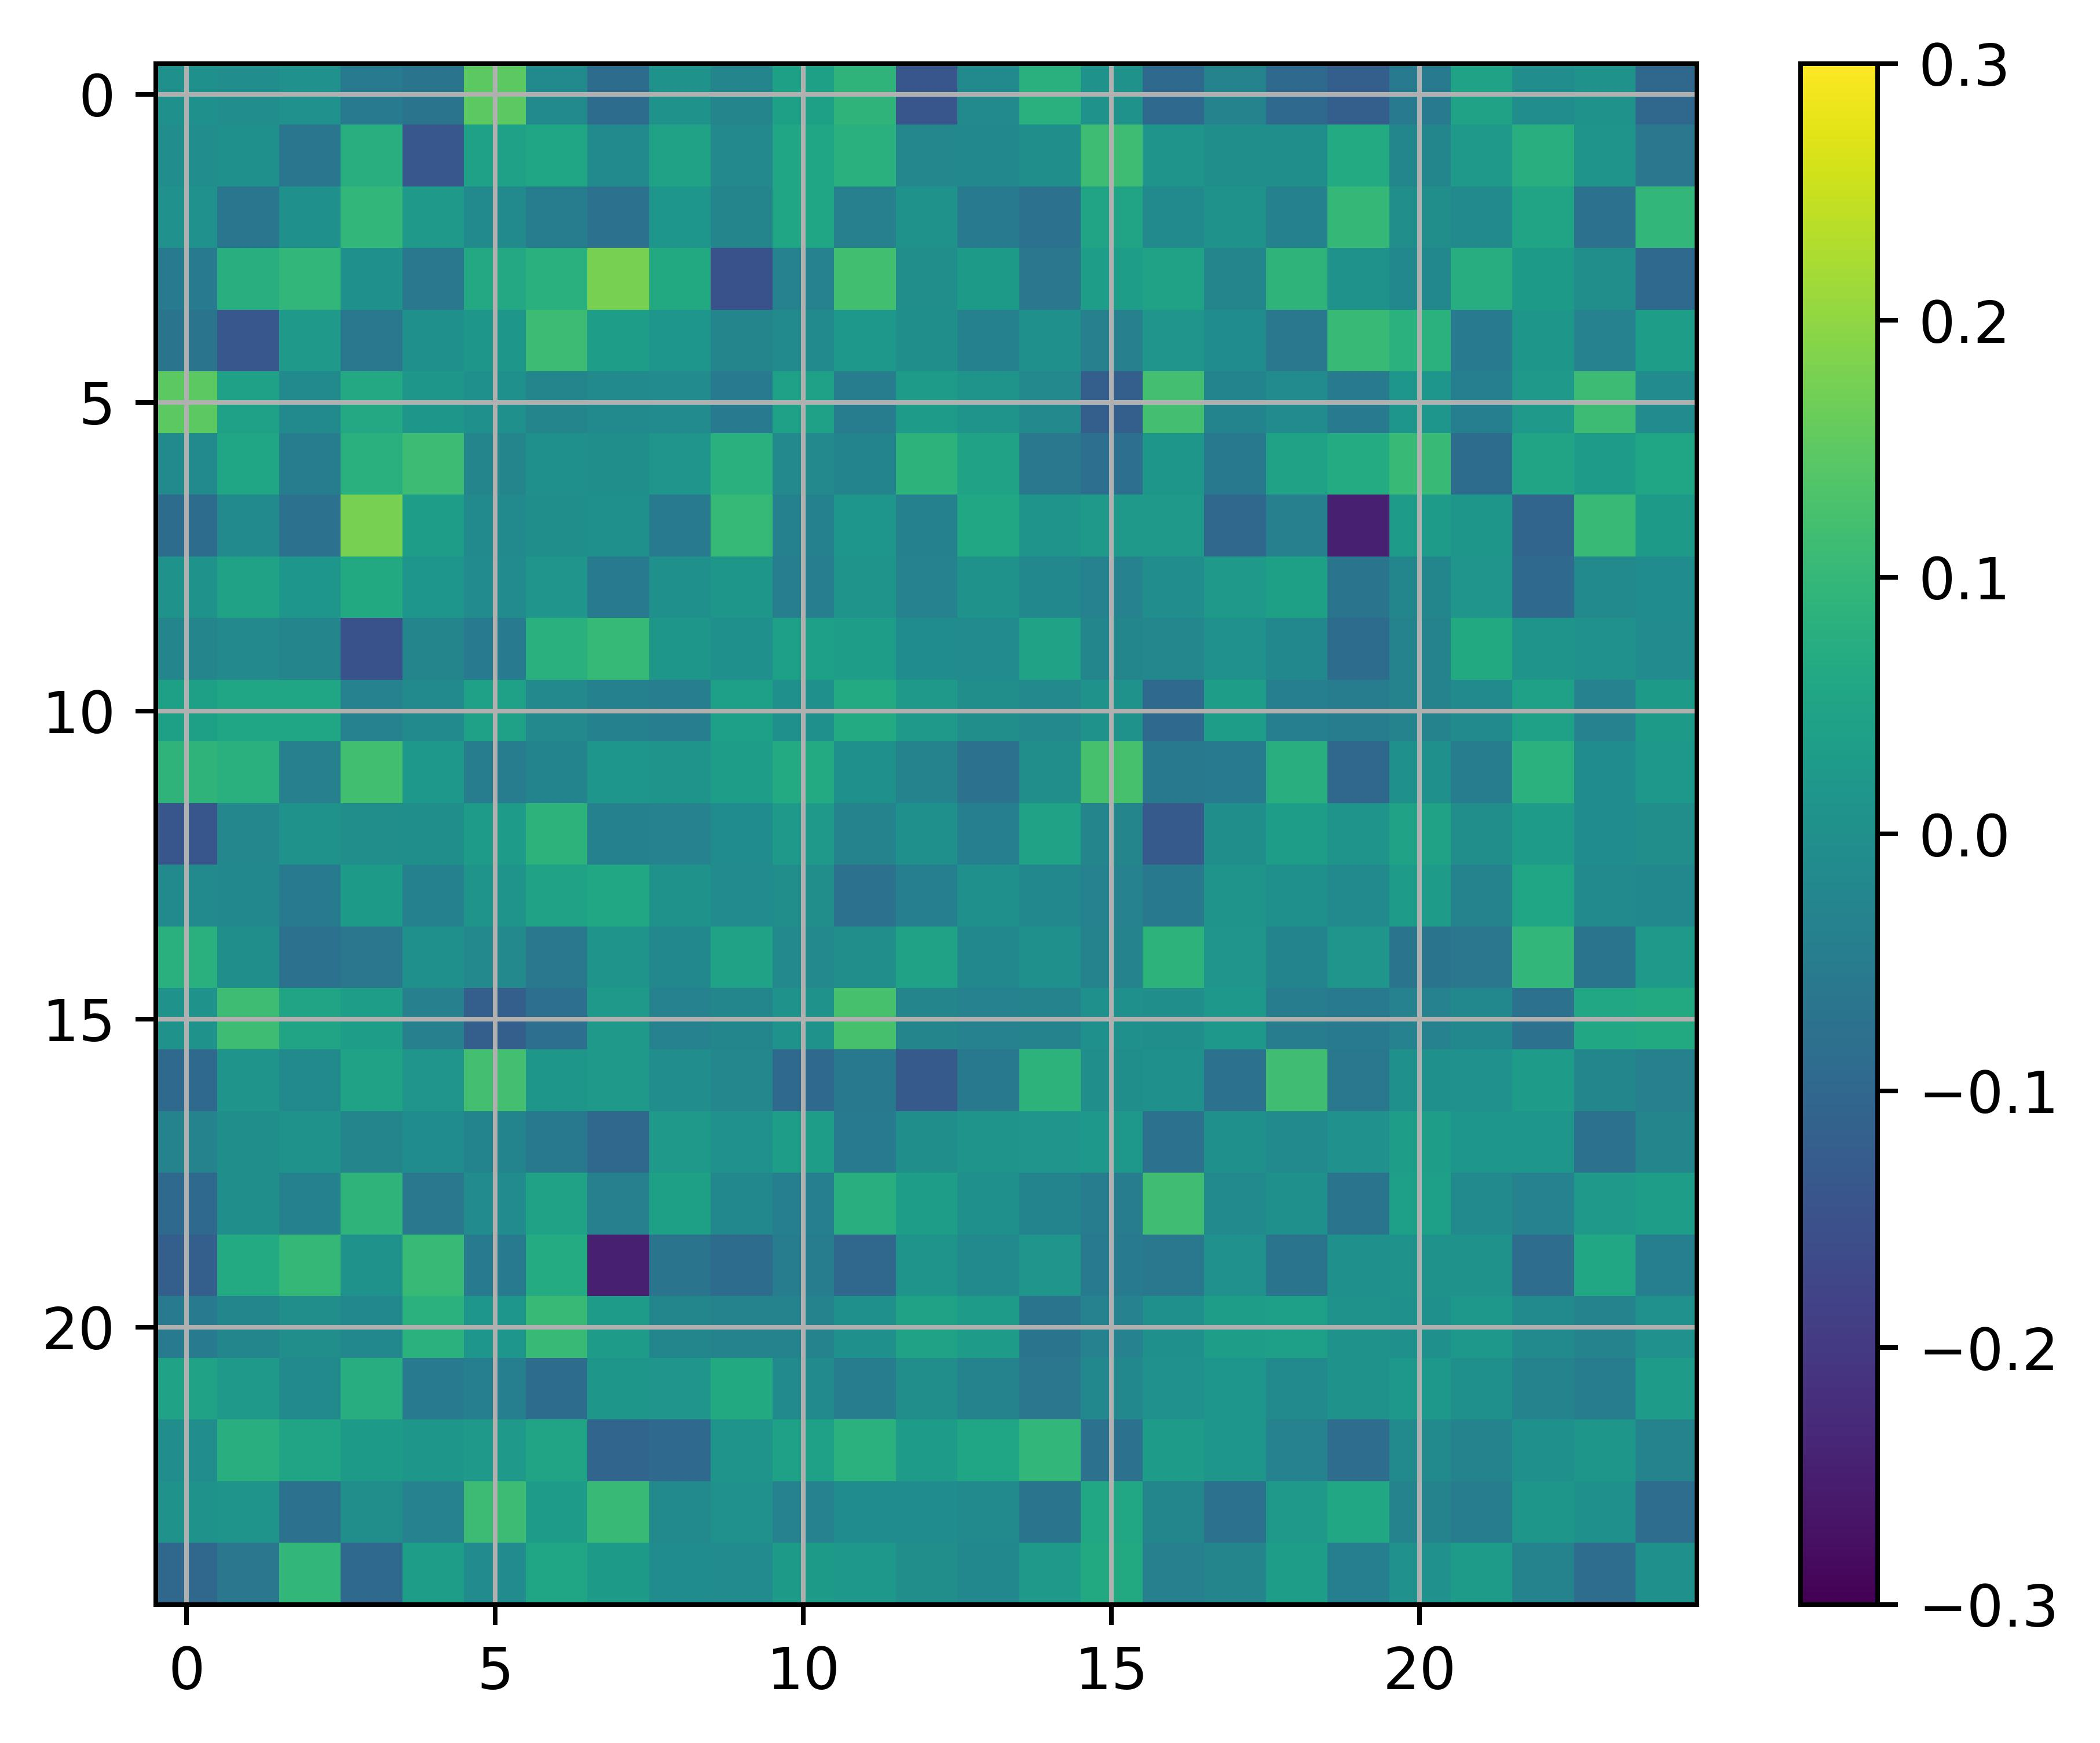
\includegraphics[width=0.2\textwidth]{../Analysis/DFC/size=480_step=180_rho=0.1/node=25_id=100206/c_12.jpg}
        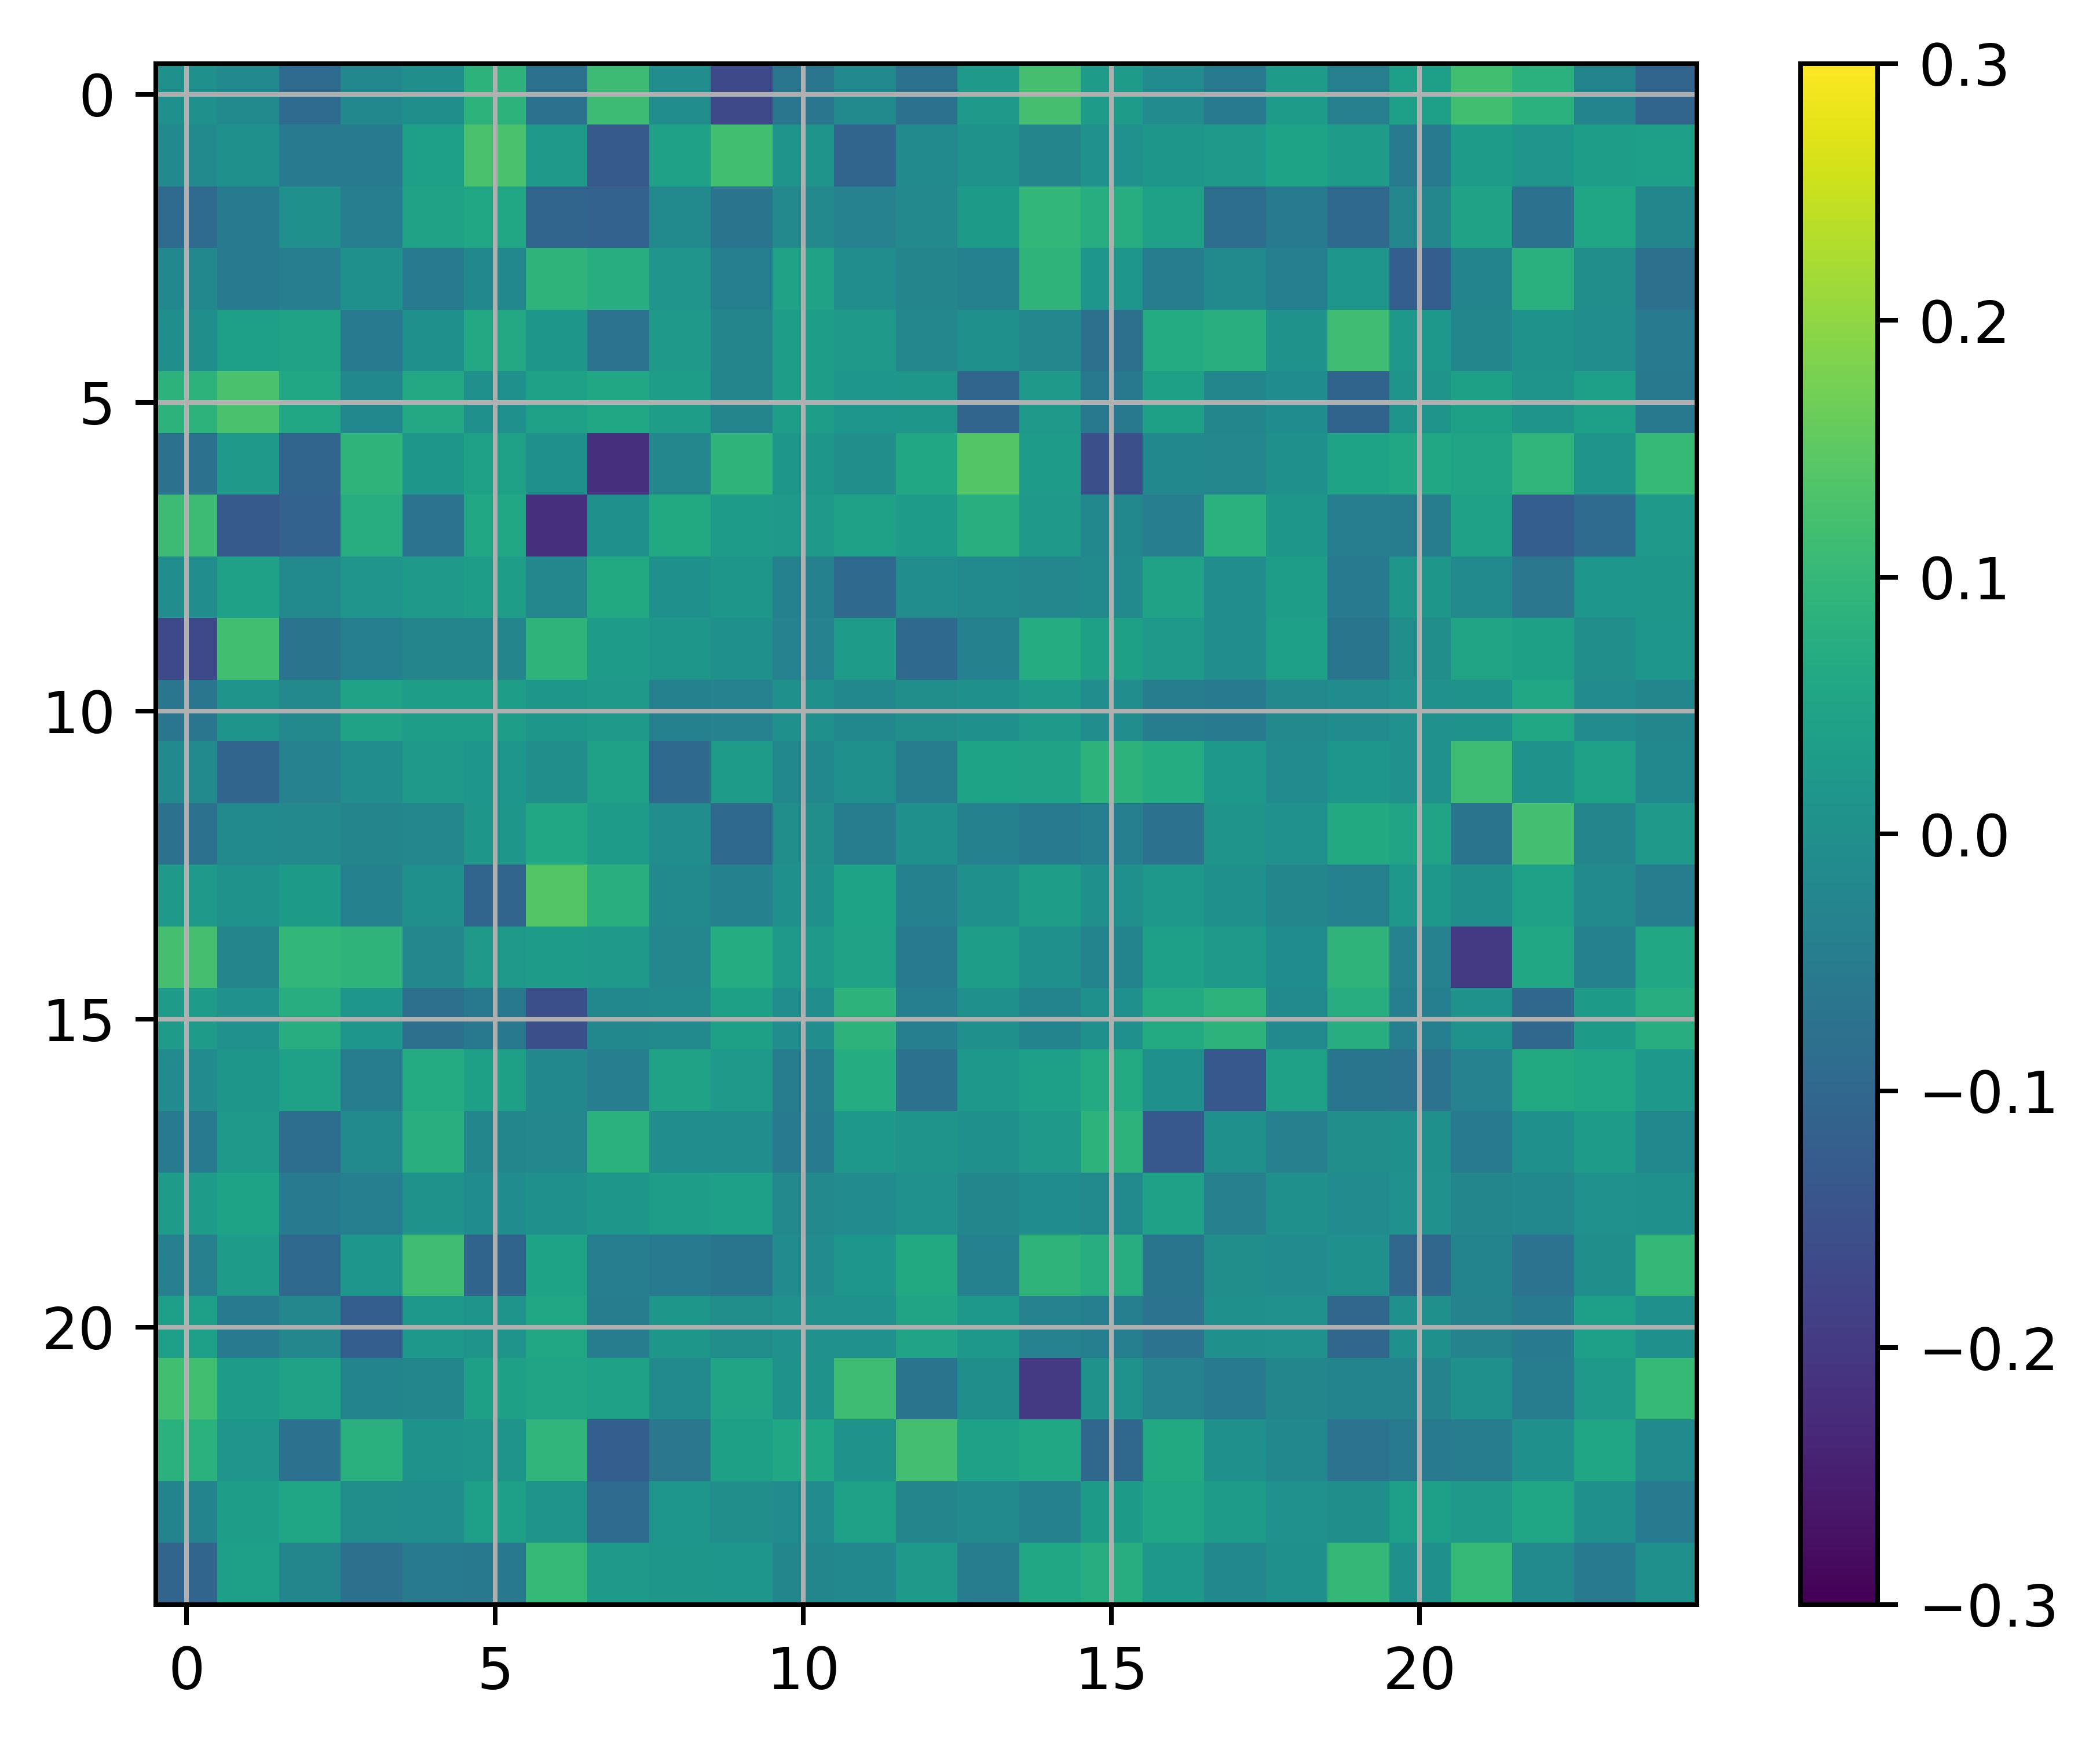
\includegraphics[width=0.2\textwidth]{../Analysis/DFC/size=480_step=180_rho=0.1/node=25_id=100206/c_14.jpg} \\
        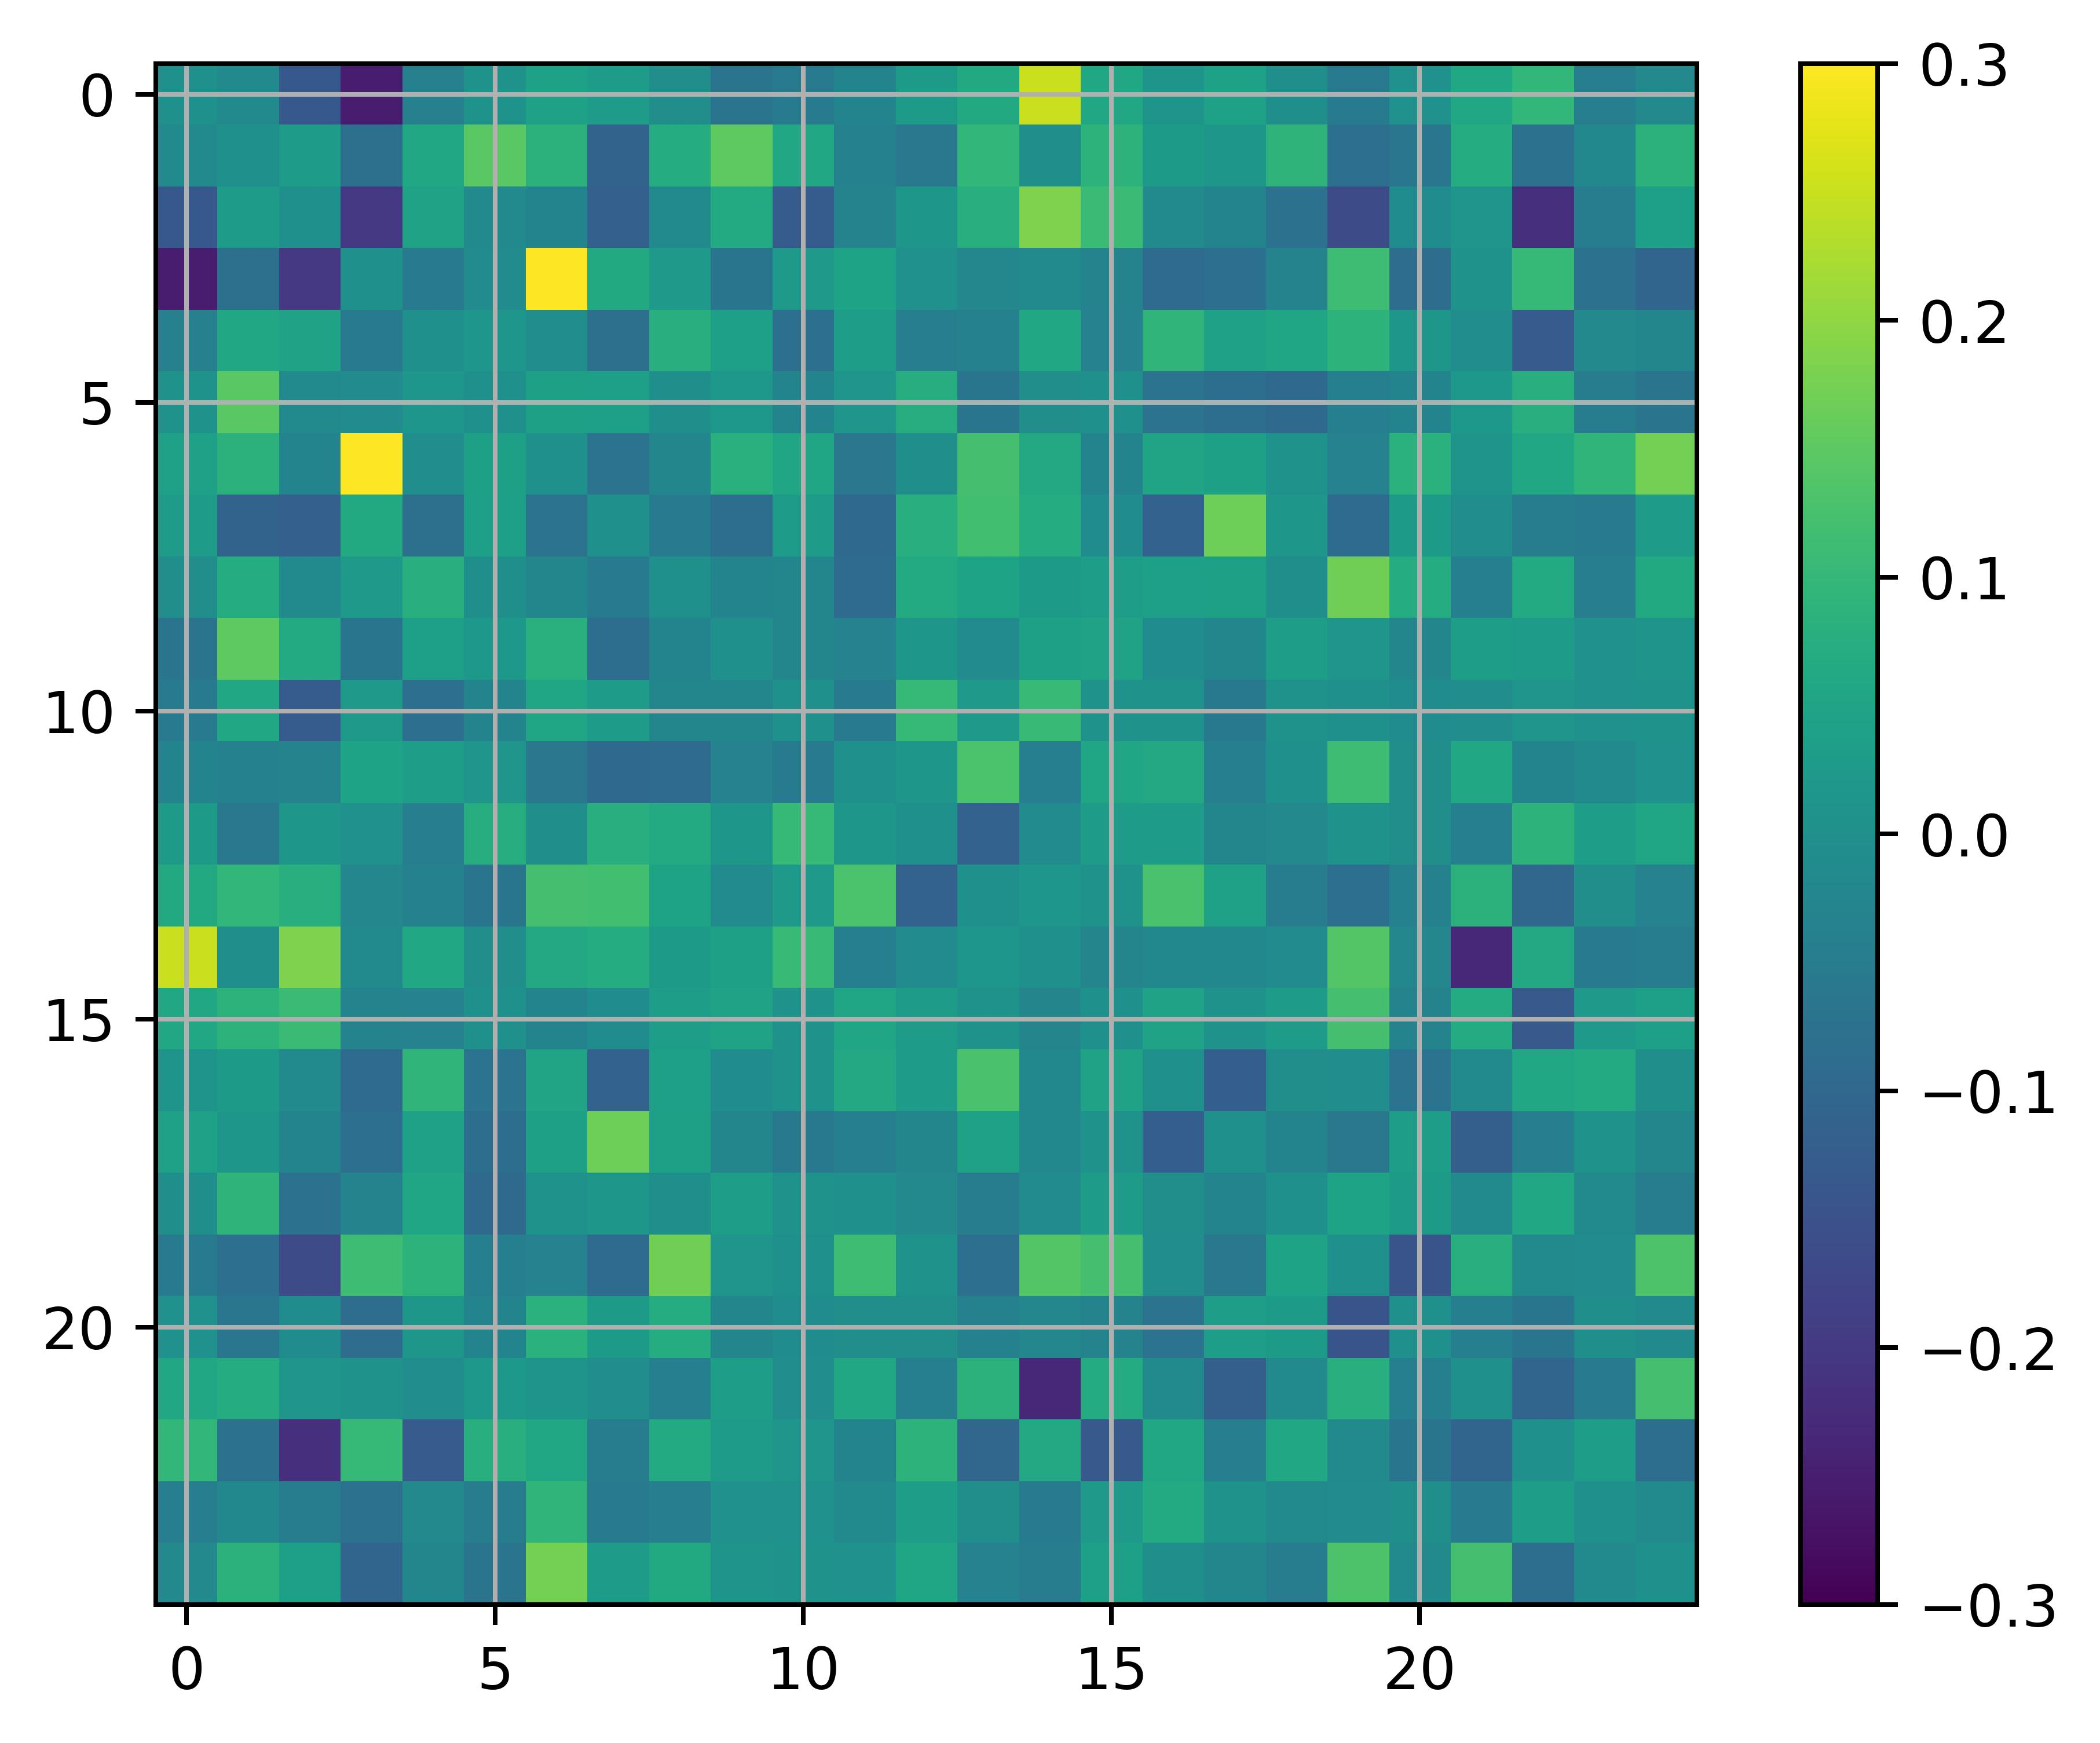
\includegraphics[width=0.2\textwidth]{../Analysis/DFC/size=480_step=180_rho=0.1/node=25_id=100206/c_16.jpg}
        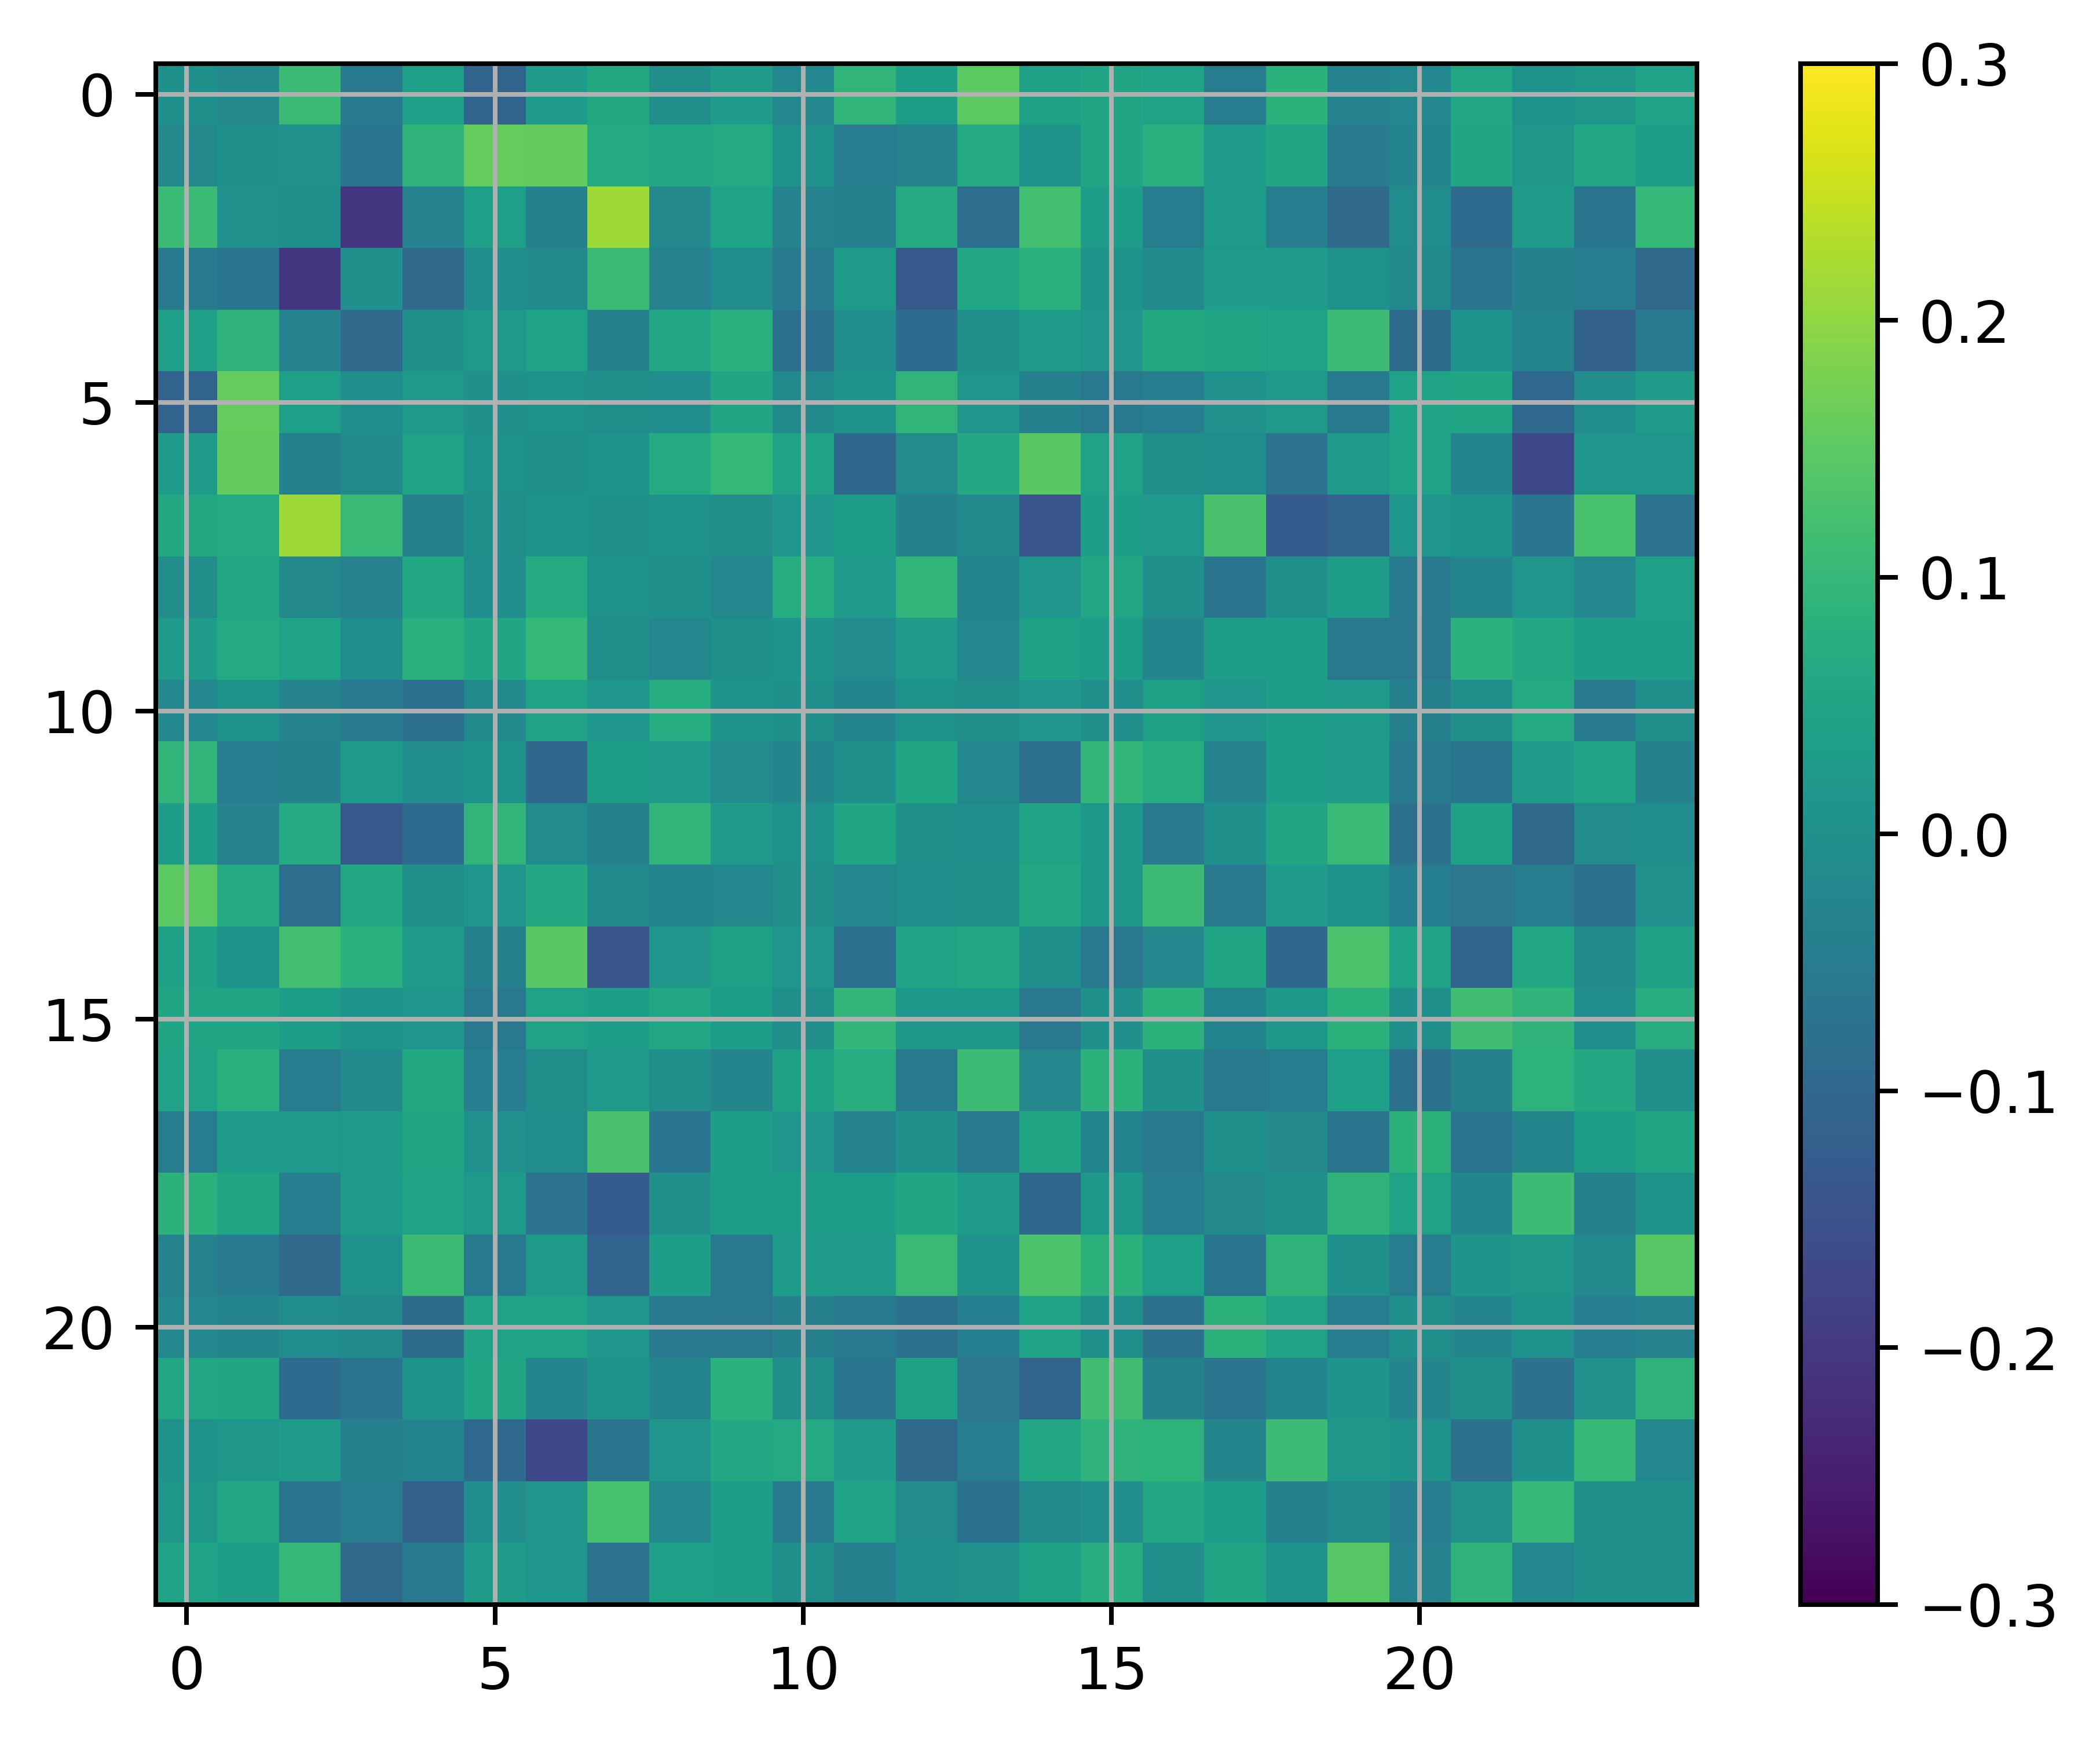
\includegraphics[width=0.2\textwidth]{../Analysis/DFC/size=480_step=180_rho=0.1/node=25_id=100206/c_18.jpg}
        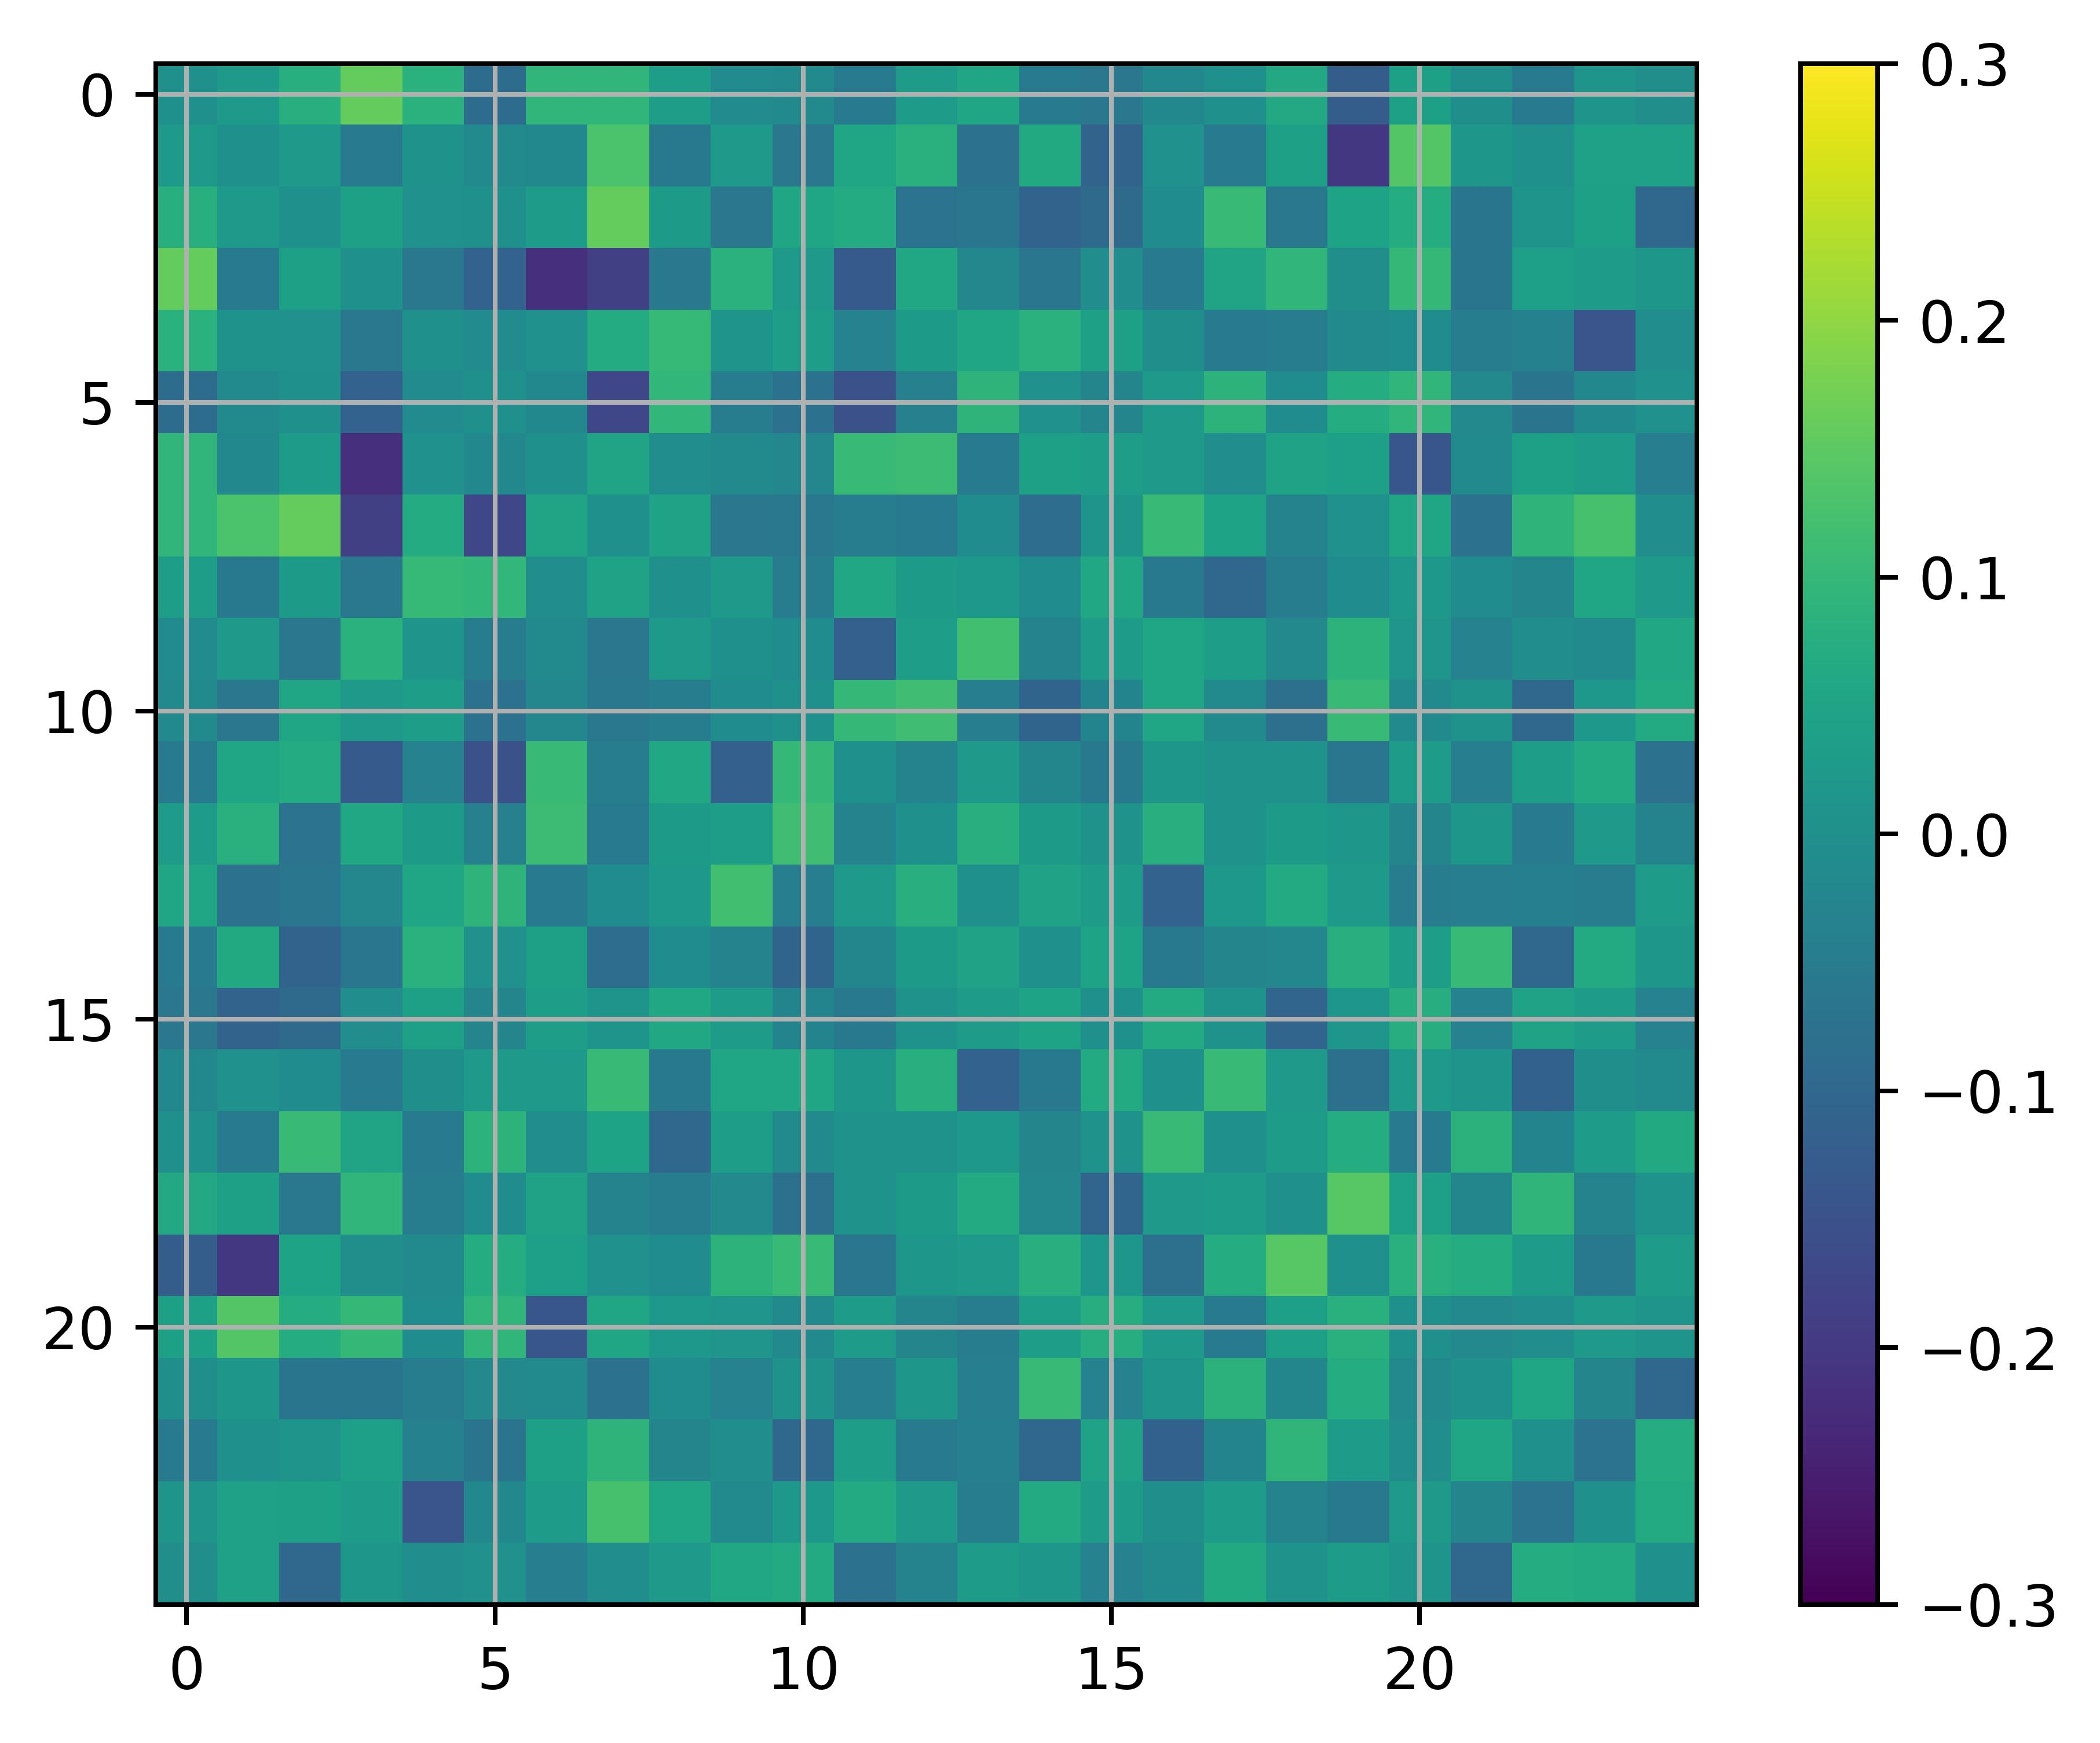
\includegraphics[width=0.2\textwidth]{../Analysis/DFC/size=480_step=180_rho=0.1/node=25_id=100206/c_20.jpg}
        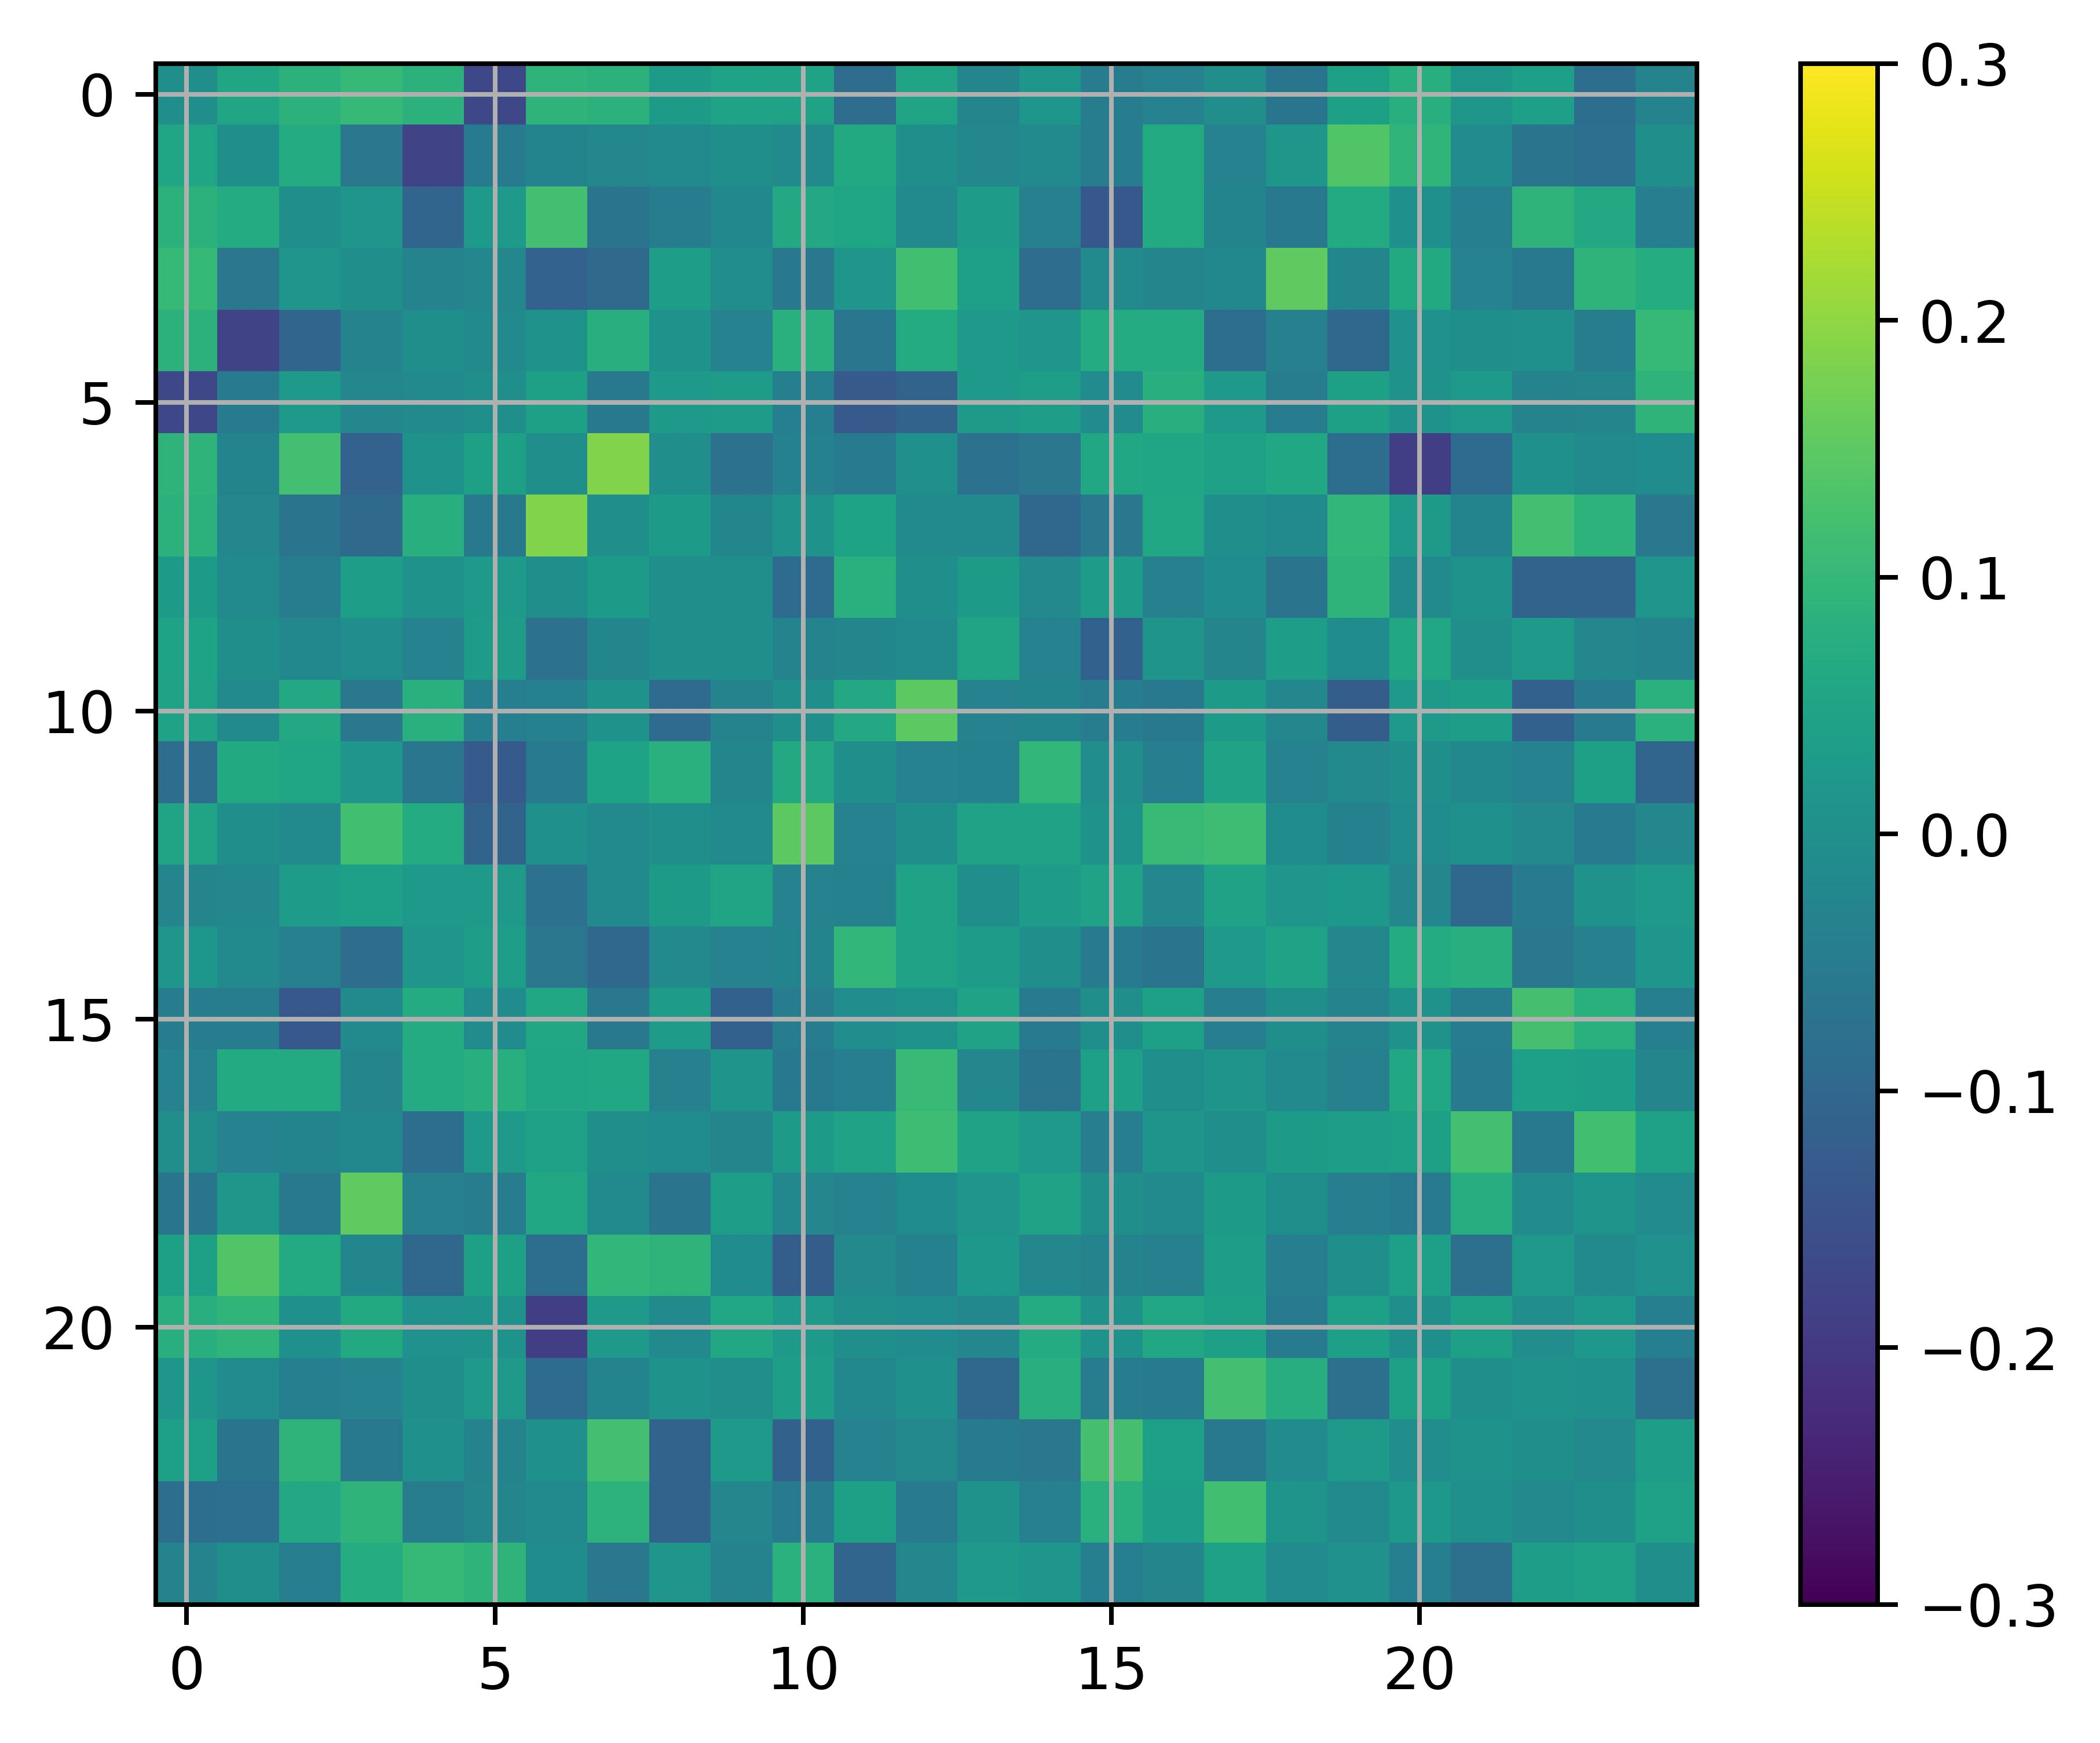
\includegraphics[width=0.2\textwidth]{../Analysis/DFC/size=480_step=180_rho=0.1/node=25_id=100206/c_22.jpg} \\
        \caption{Centered dynamic functional connectivity with $N_{node} = 25$.}
        % \label{LDA-example-1}
    \end{figure}

\end{frame}

\begin{frame}{Preprocessing - Examples}

    \begin{figure}[H]
        \centering
        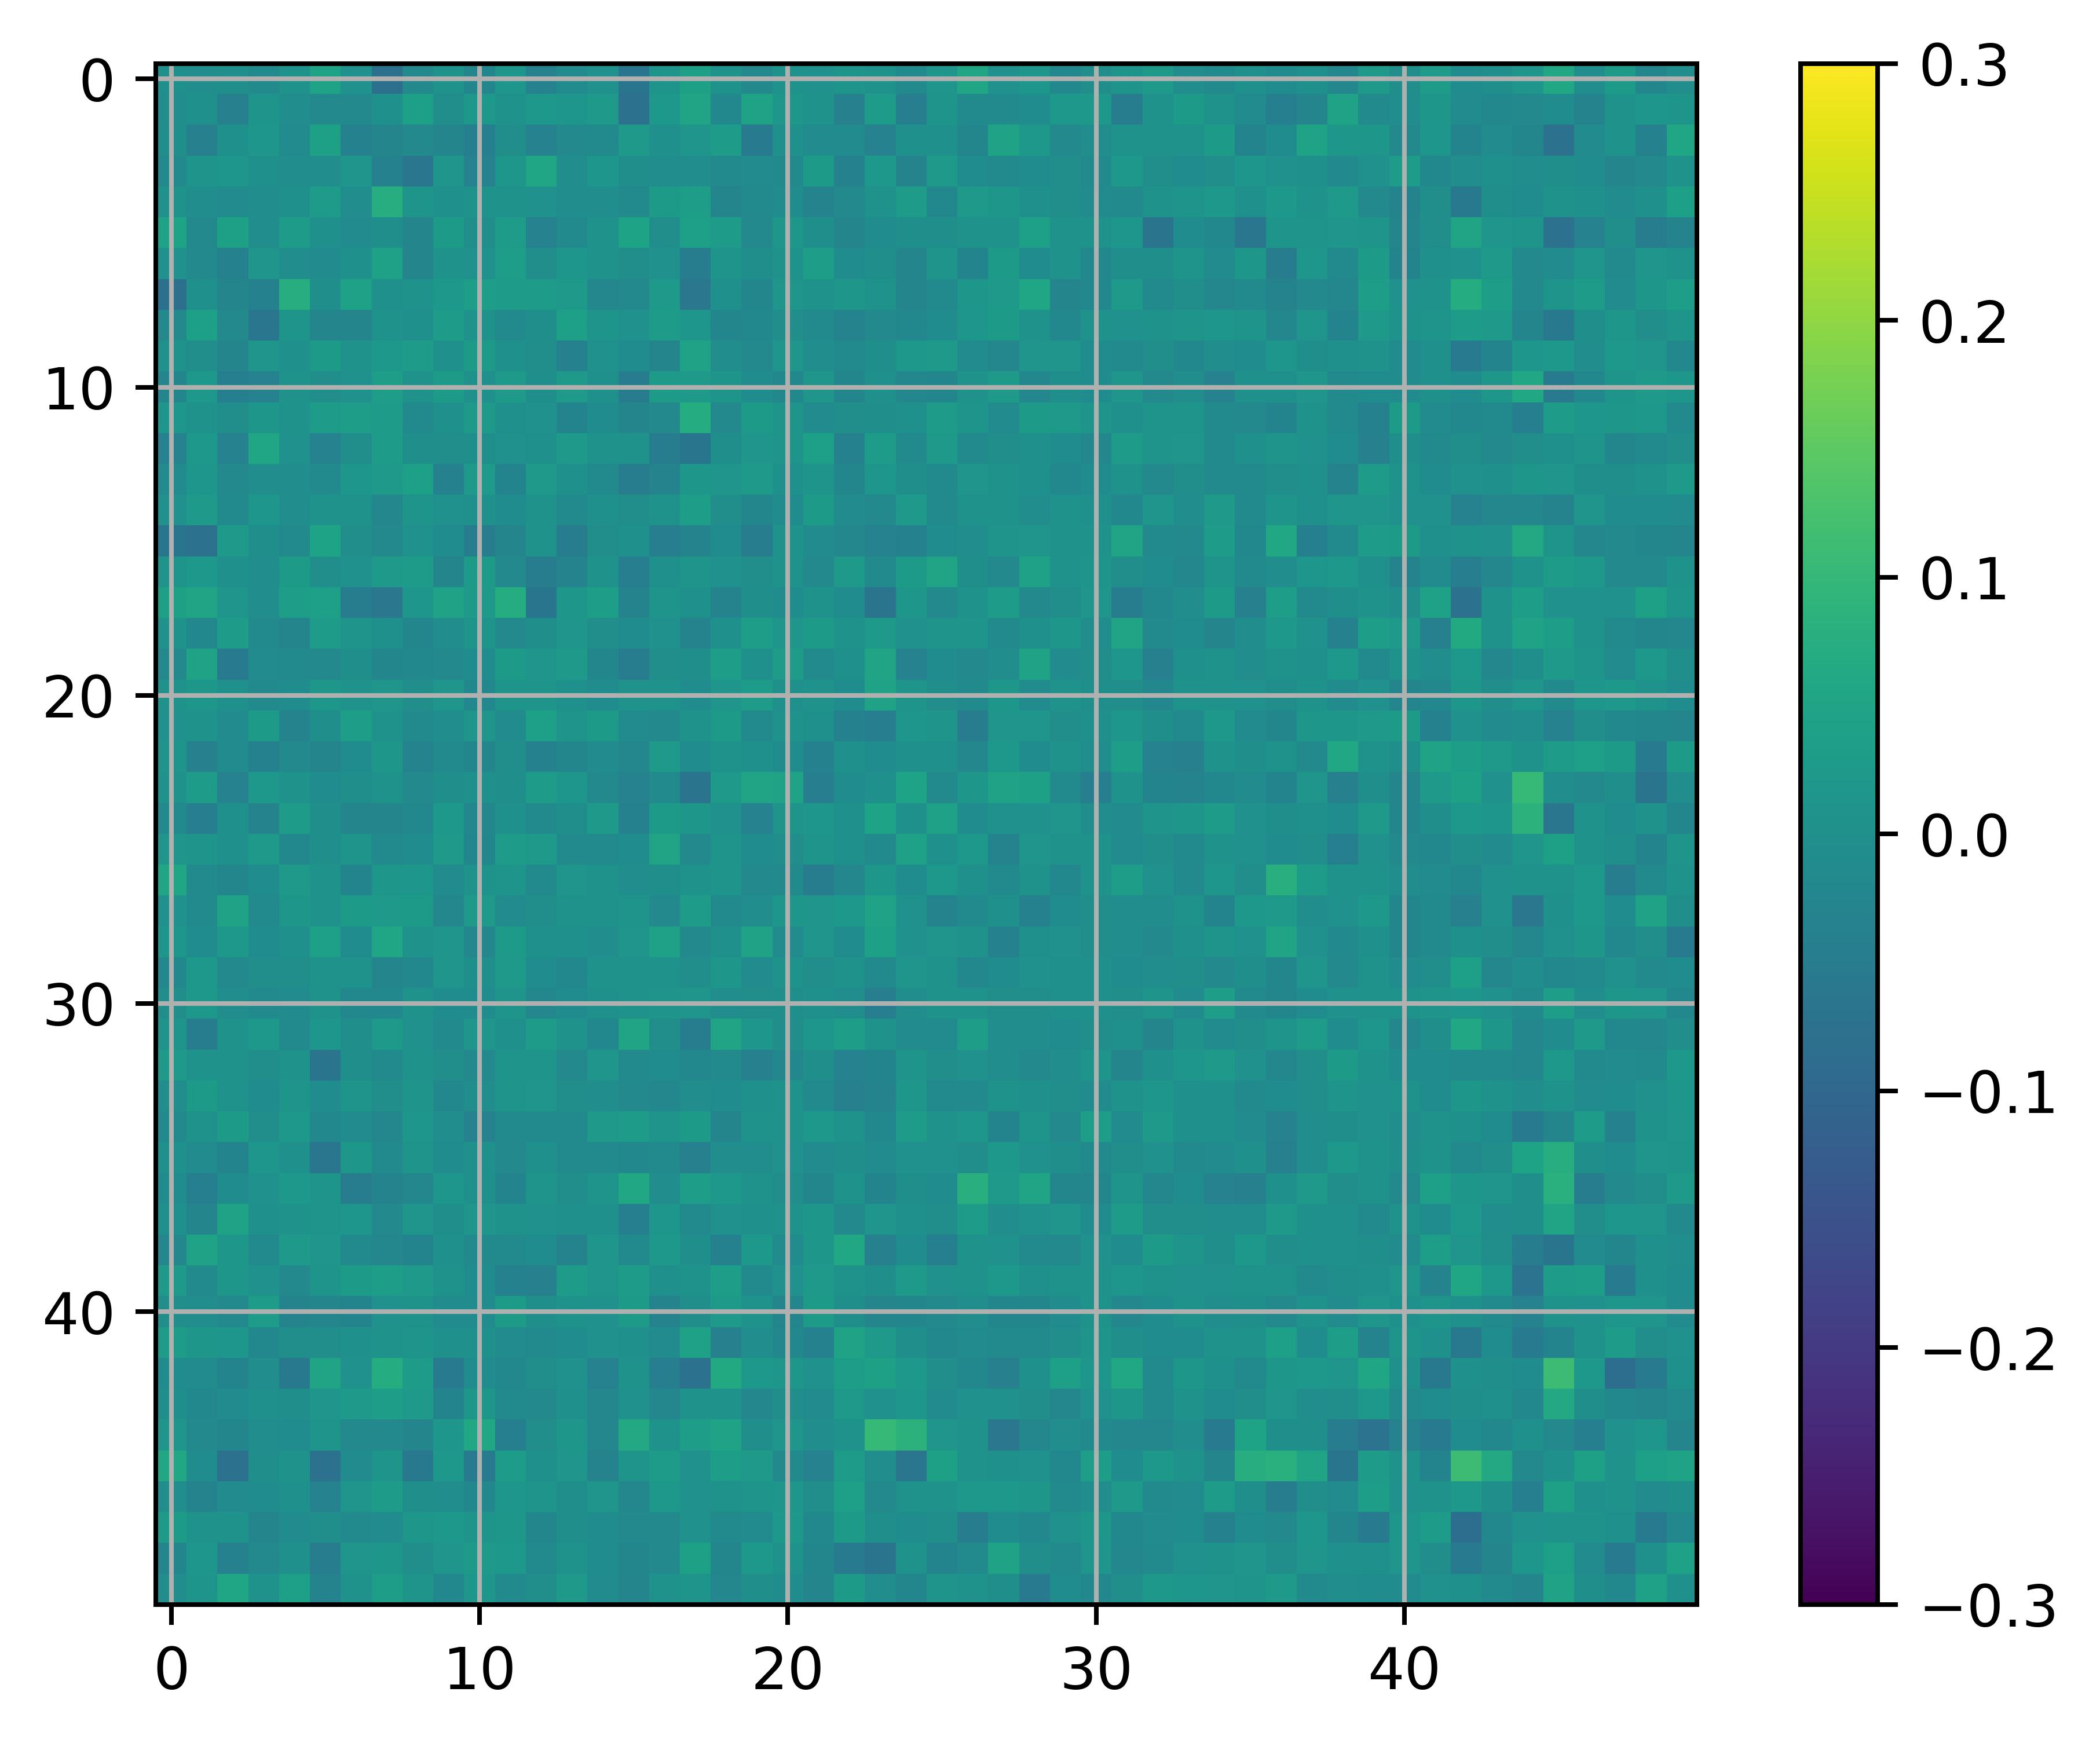
\includegraphics[width=0.2\textwidth]{../Analysis/DFC/size=480_step=180_rho=0.1/node=50_id=100206/c_0.jpg}
        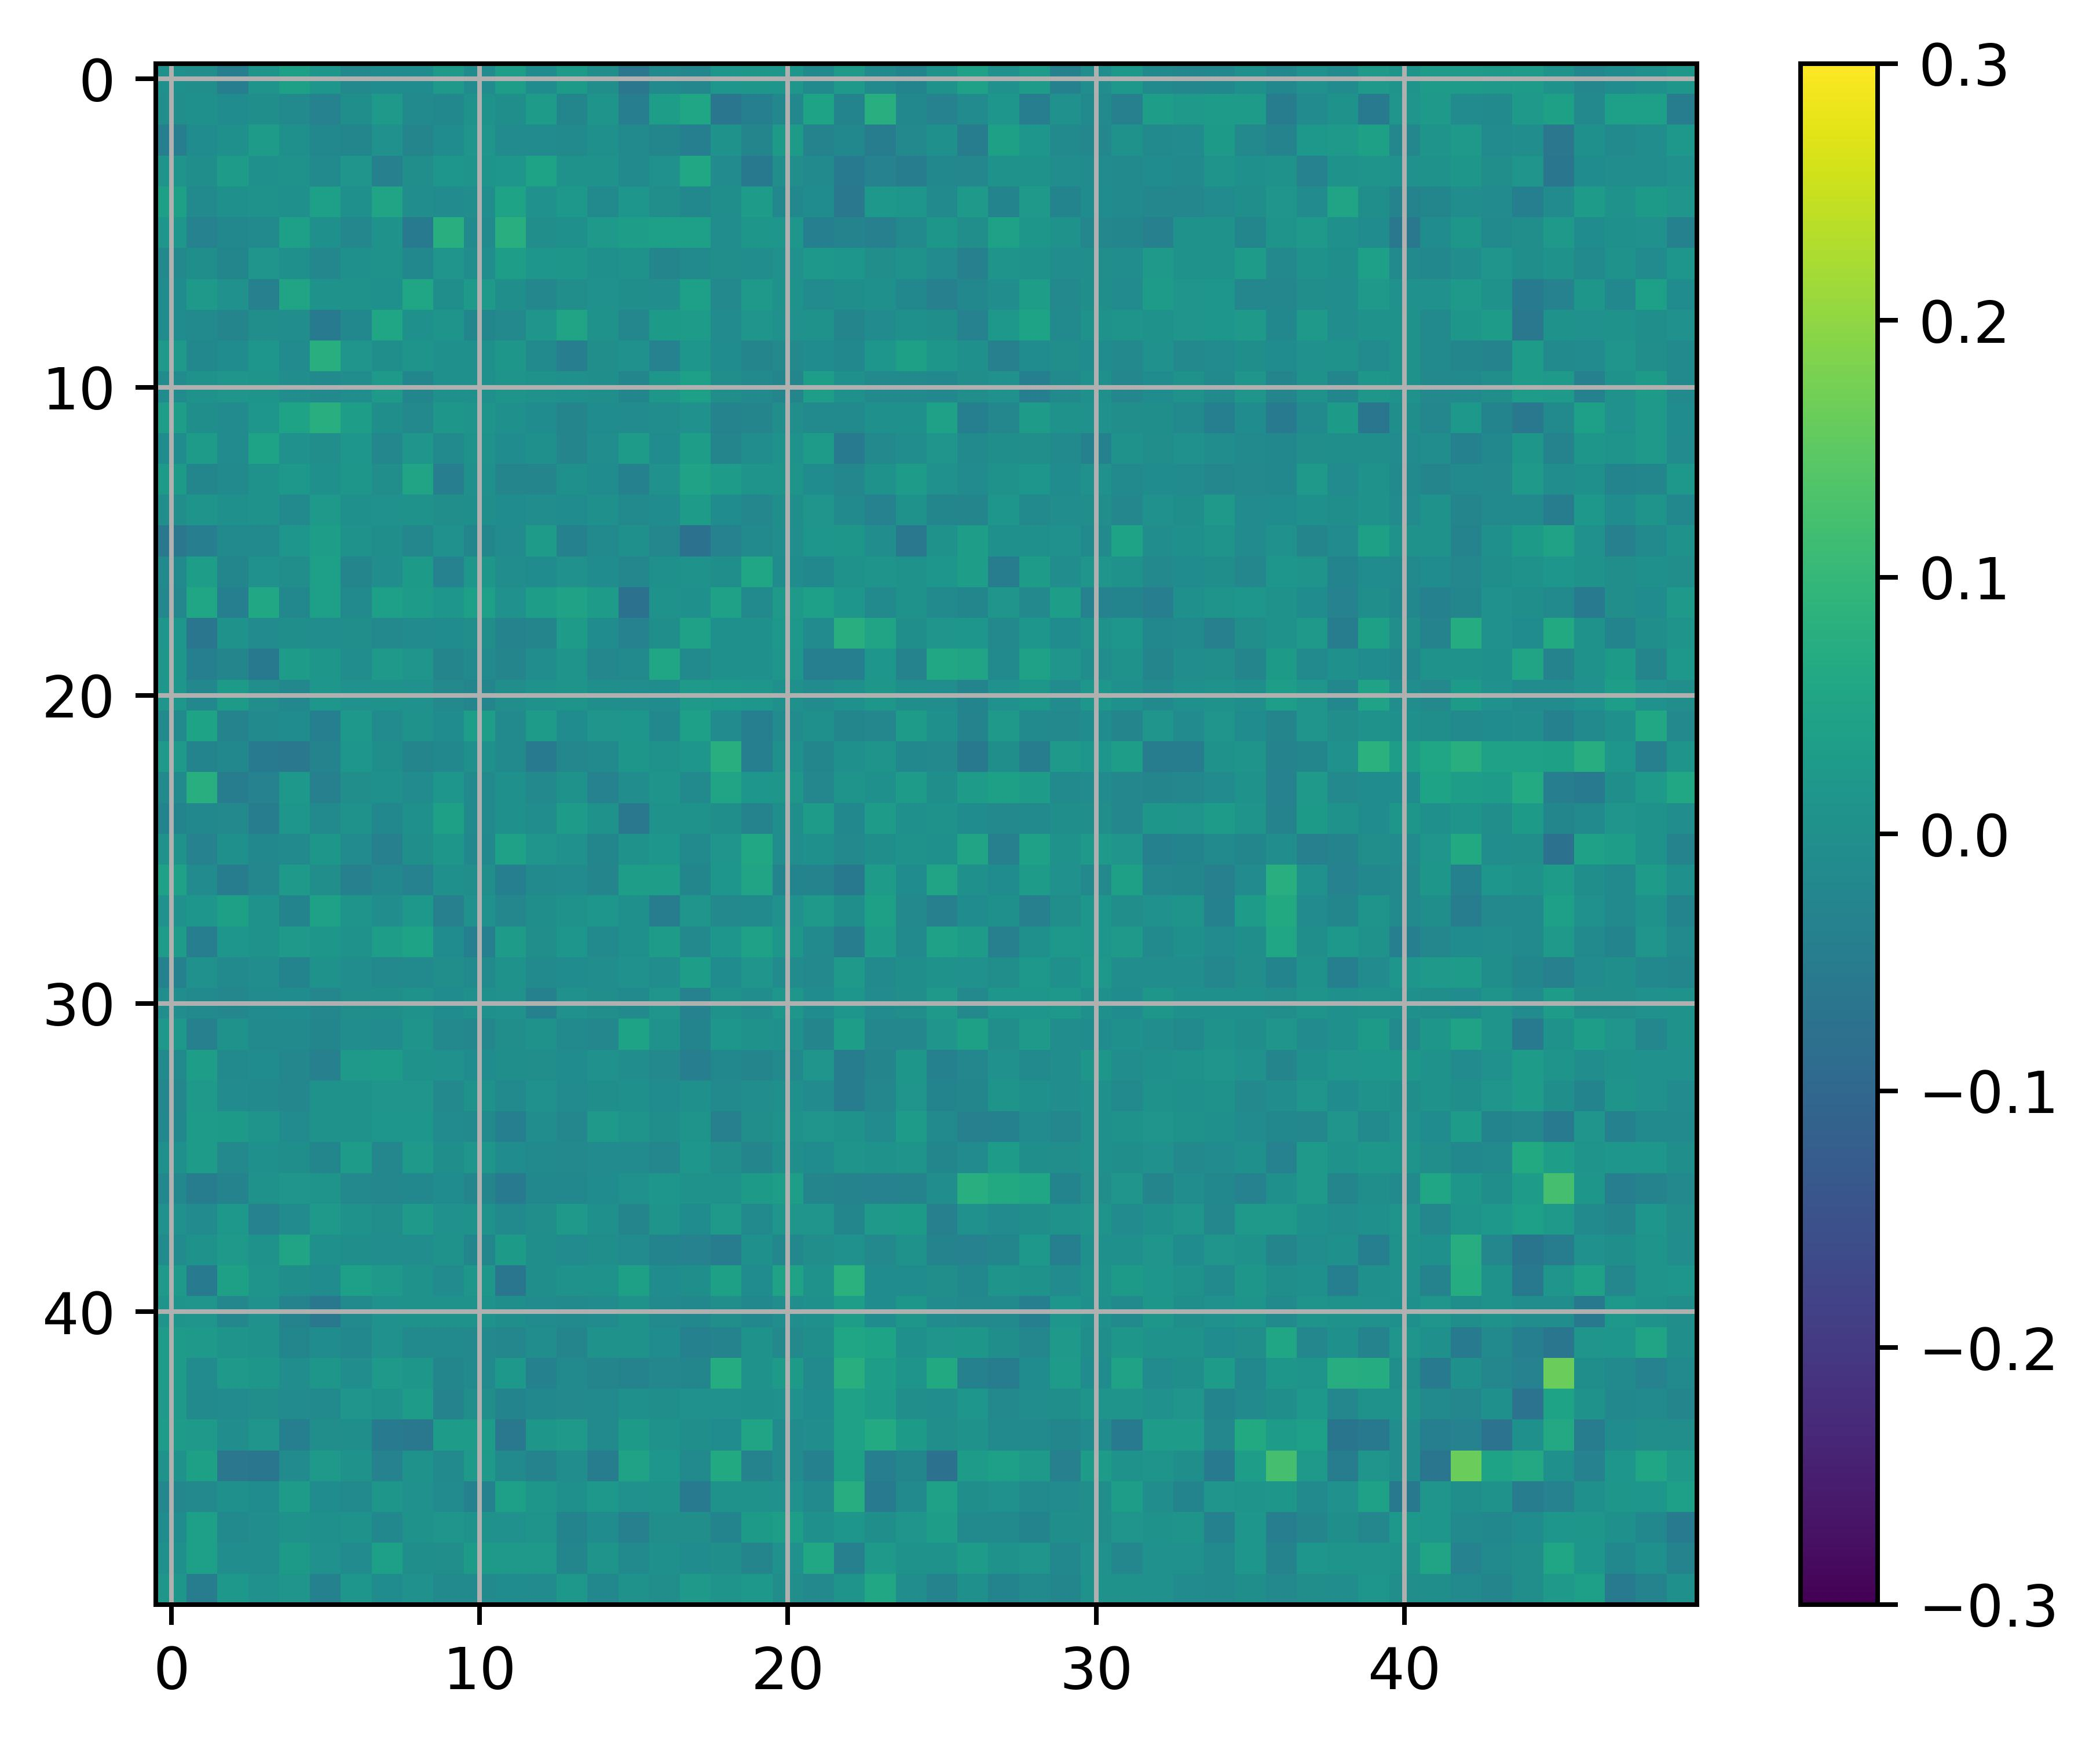
\includegraphics[width=0.2\textwidth]{../Analysis/DFC/size=480_step=180_rho=0.1/node=50_id=100206/c_2.jpg}
        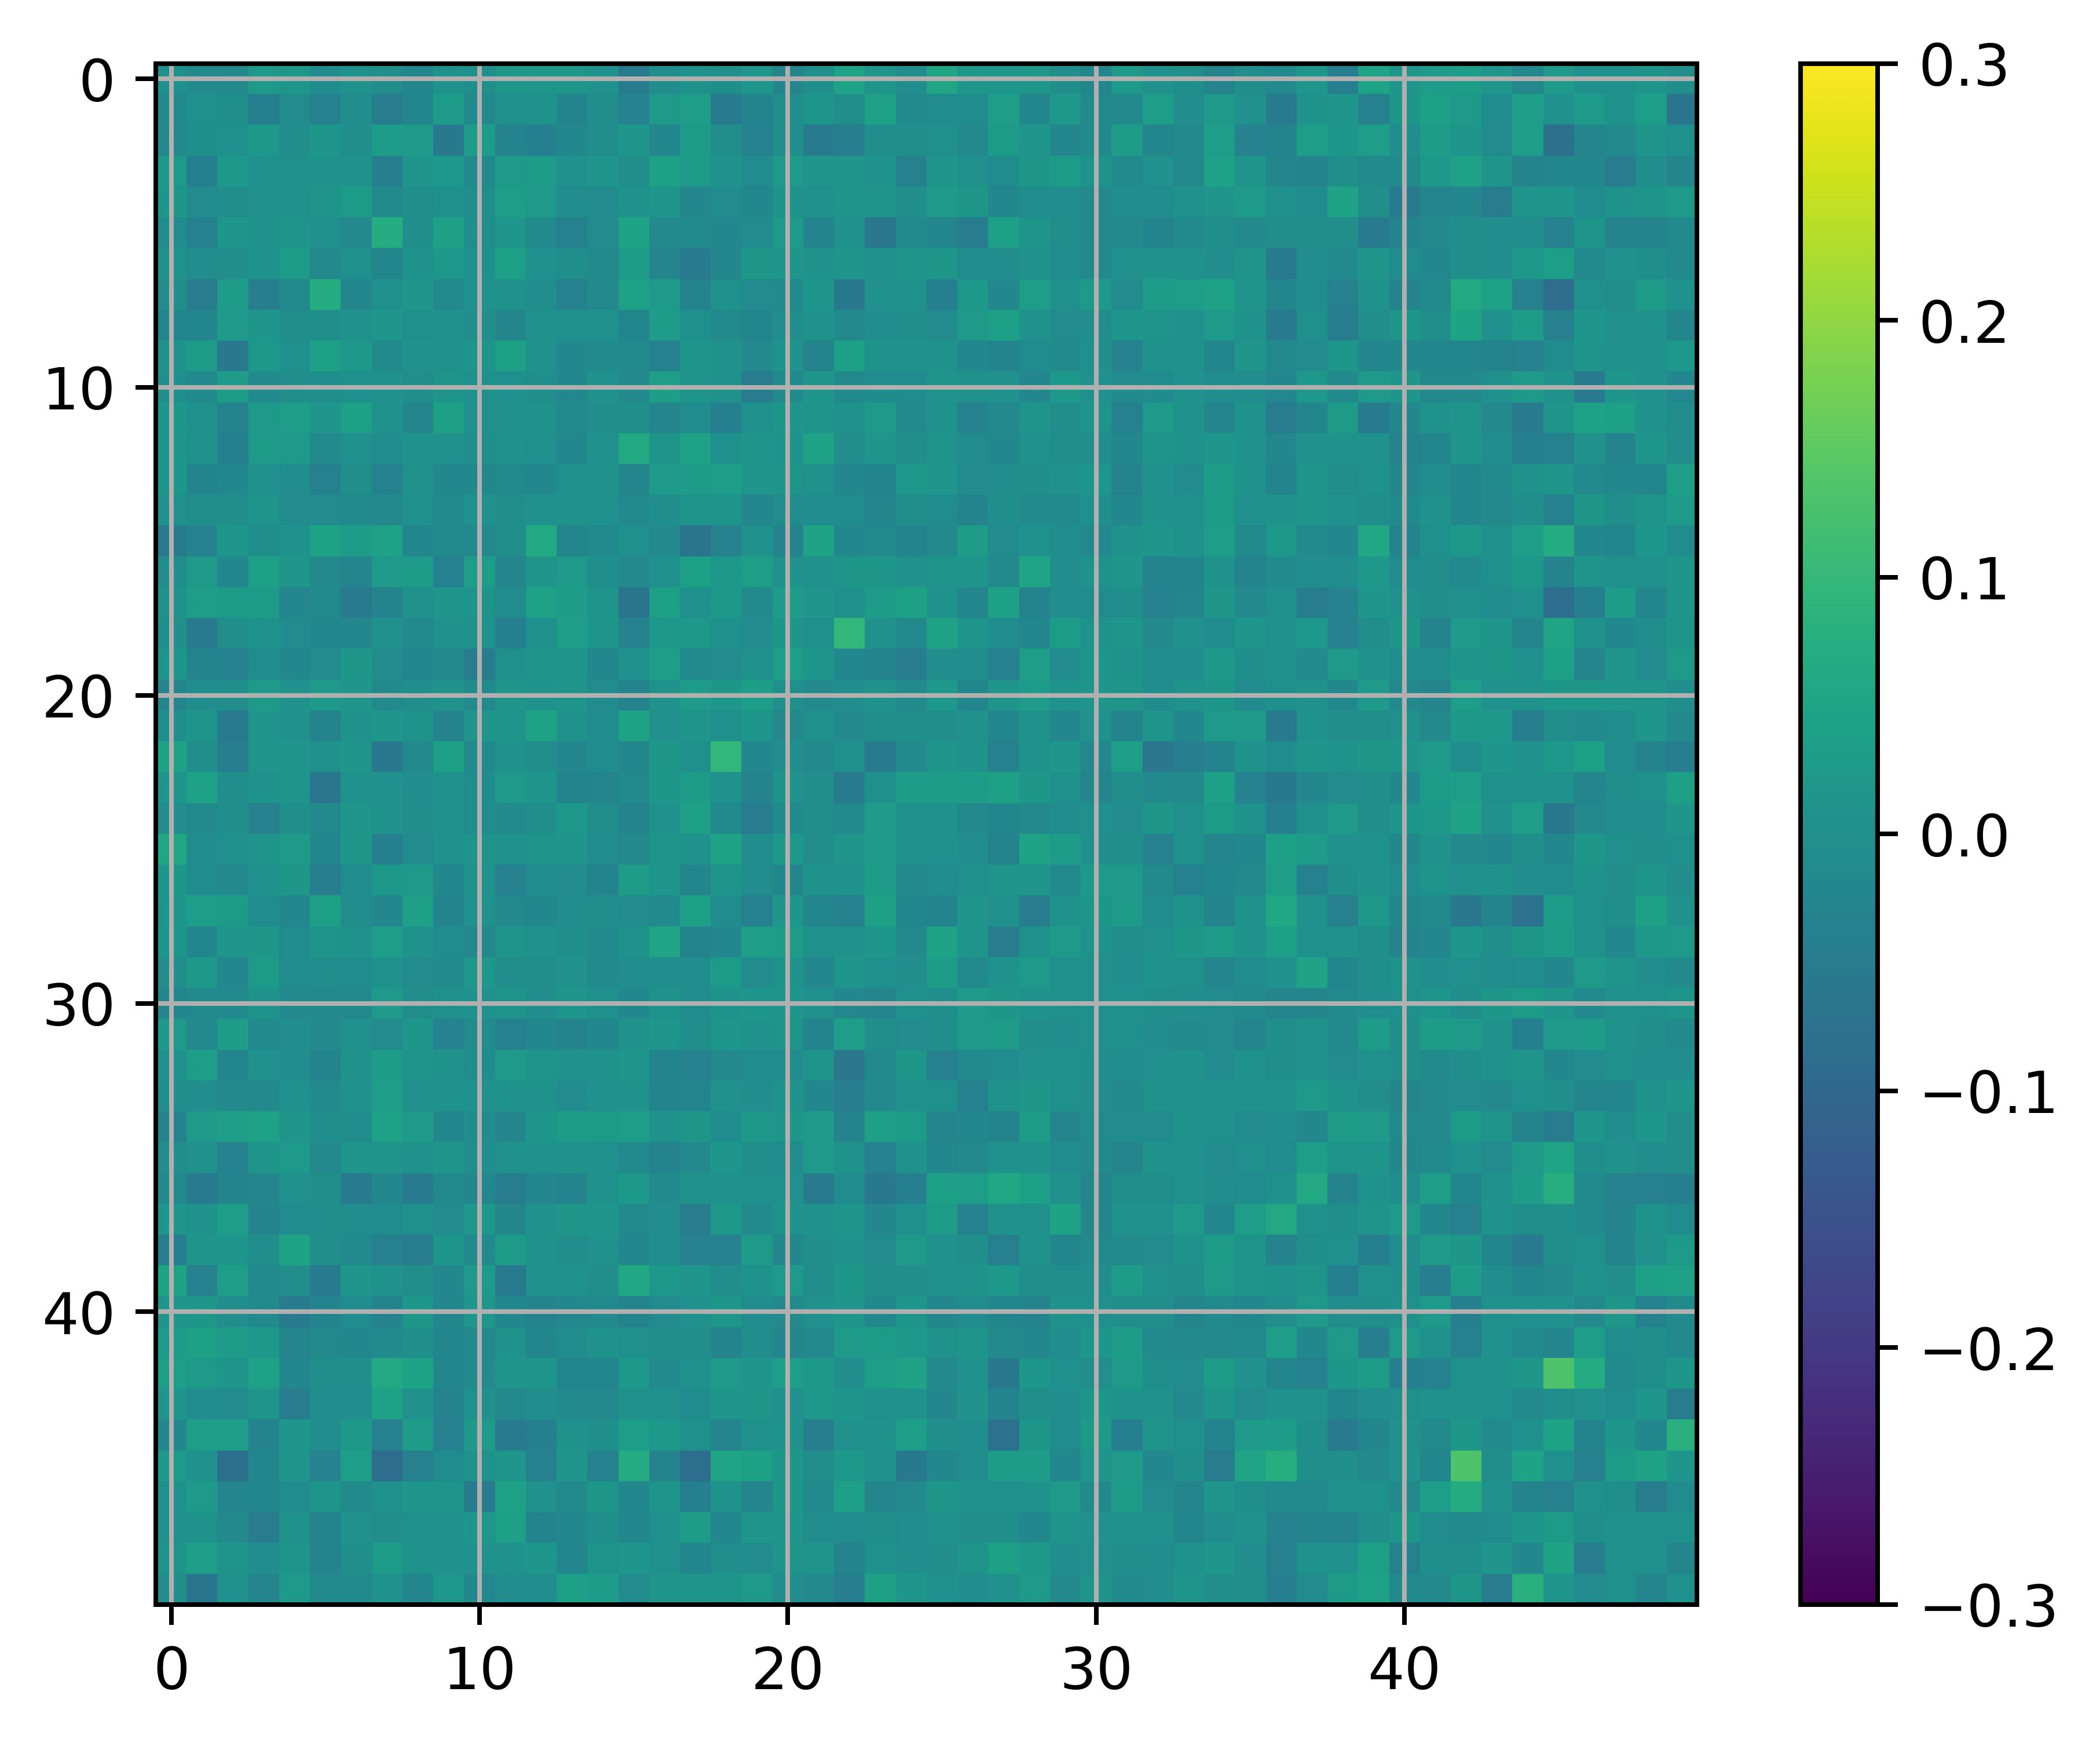
\includegraphics[width=0.2\textwidth]{../Analysis/DFC/size=480_step=180_rho=0.1/node=50_id=100206/c_4.jpg}
        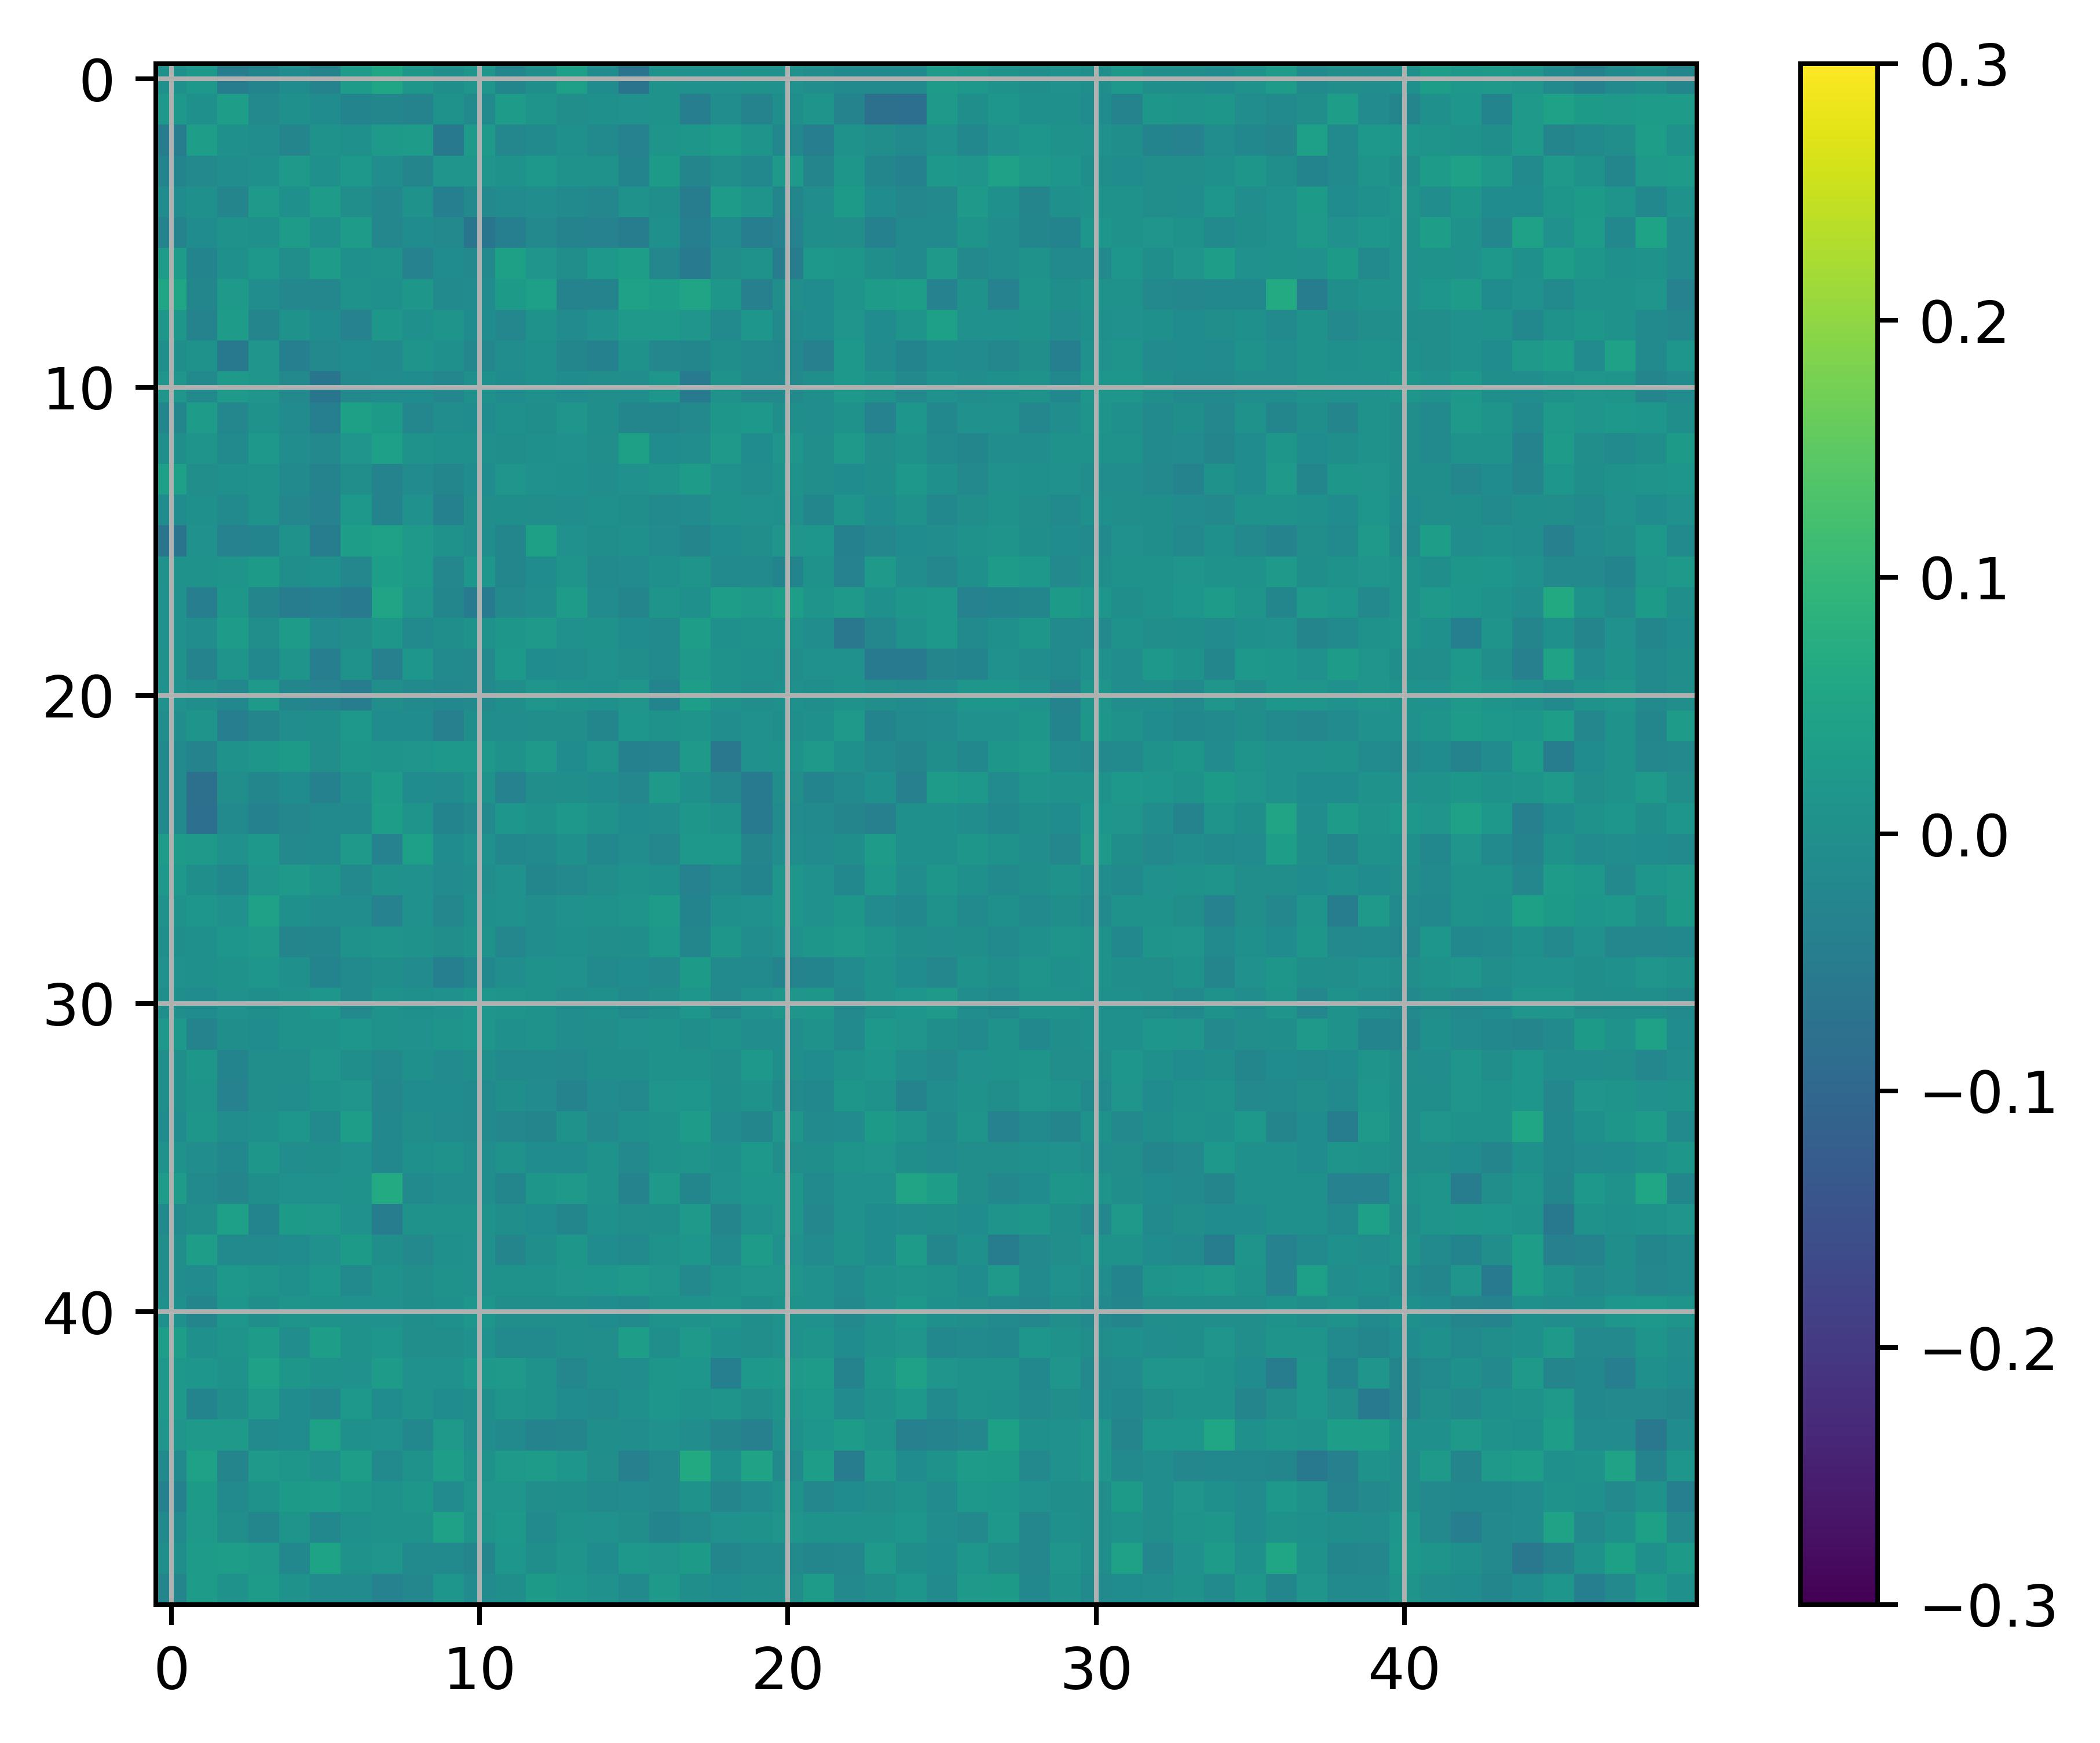
\includegraphics[width=0.2\textwidth]{../Analysis/DFC/size=480_step=180_rho=0.1/node=50_id=100206/c_6.jpg} \\
        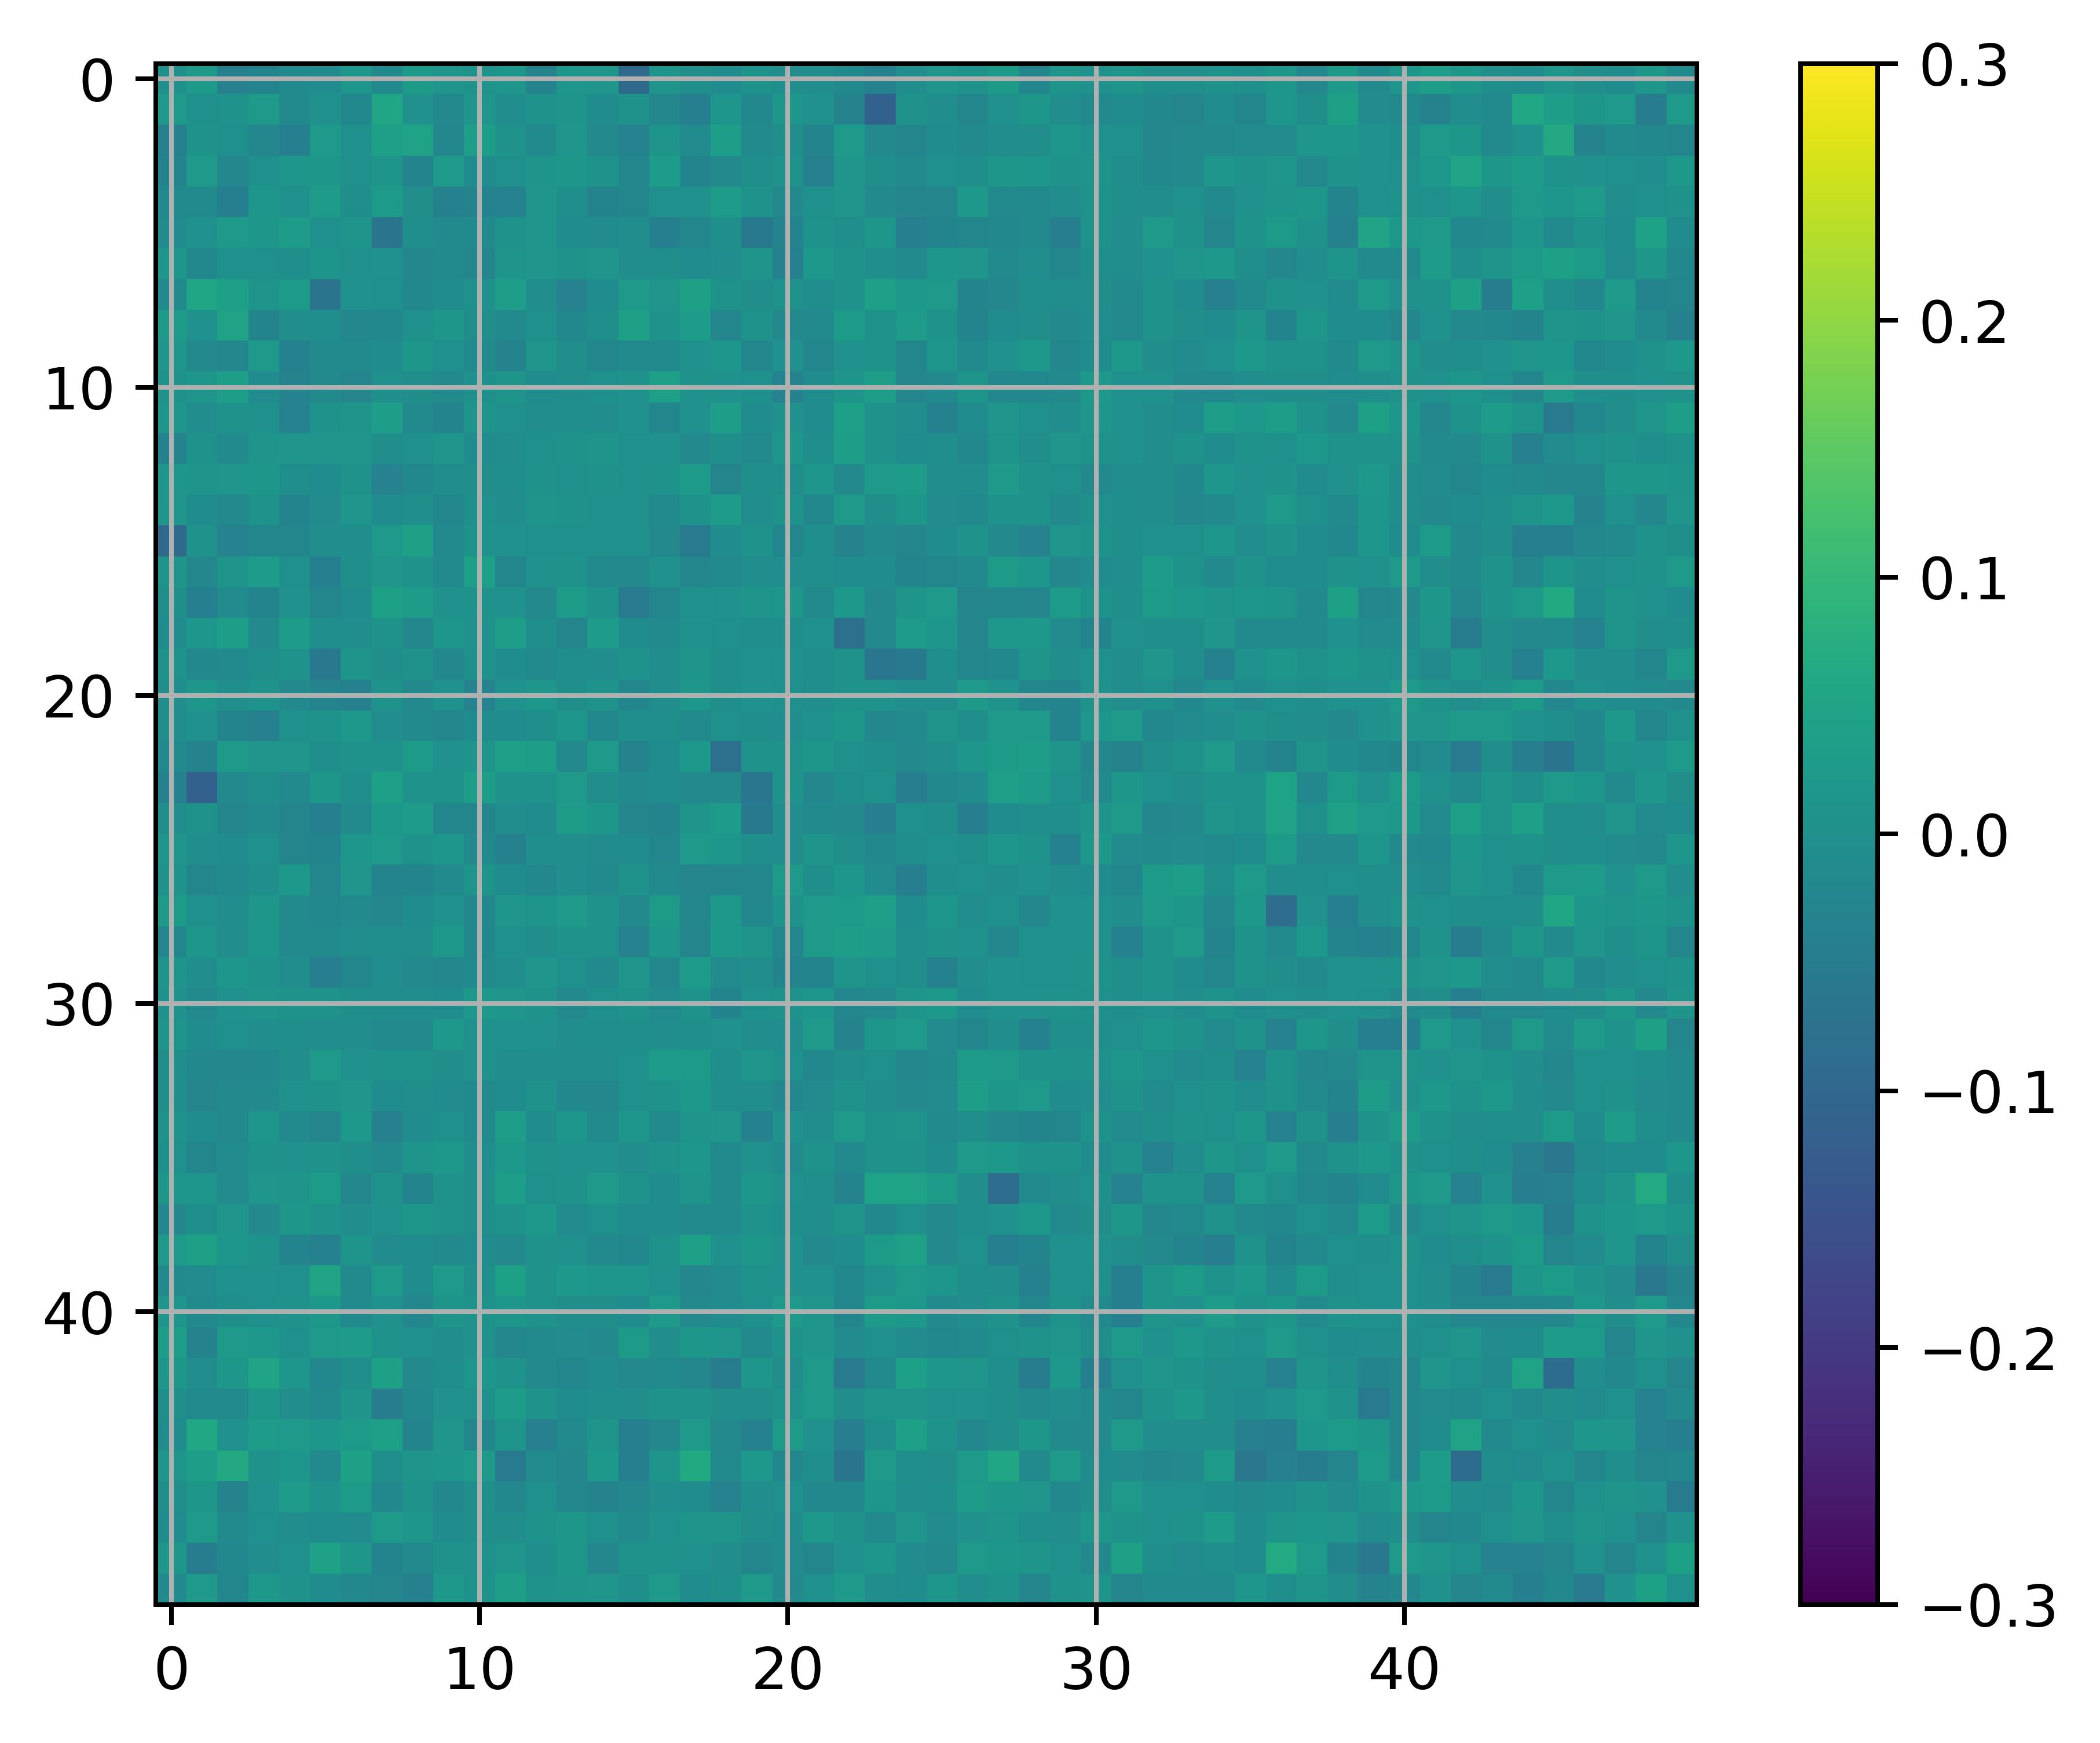
\includegraphics[width=0.2\textwidth]{../Analysis/DFC/size=480_step=180_rho=0.1/node=50_id=100206/c_8.jpg}
        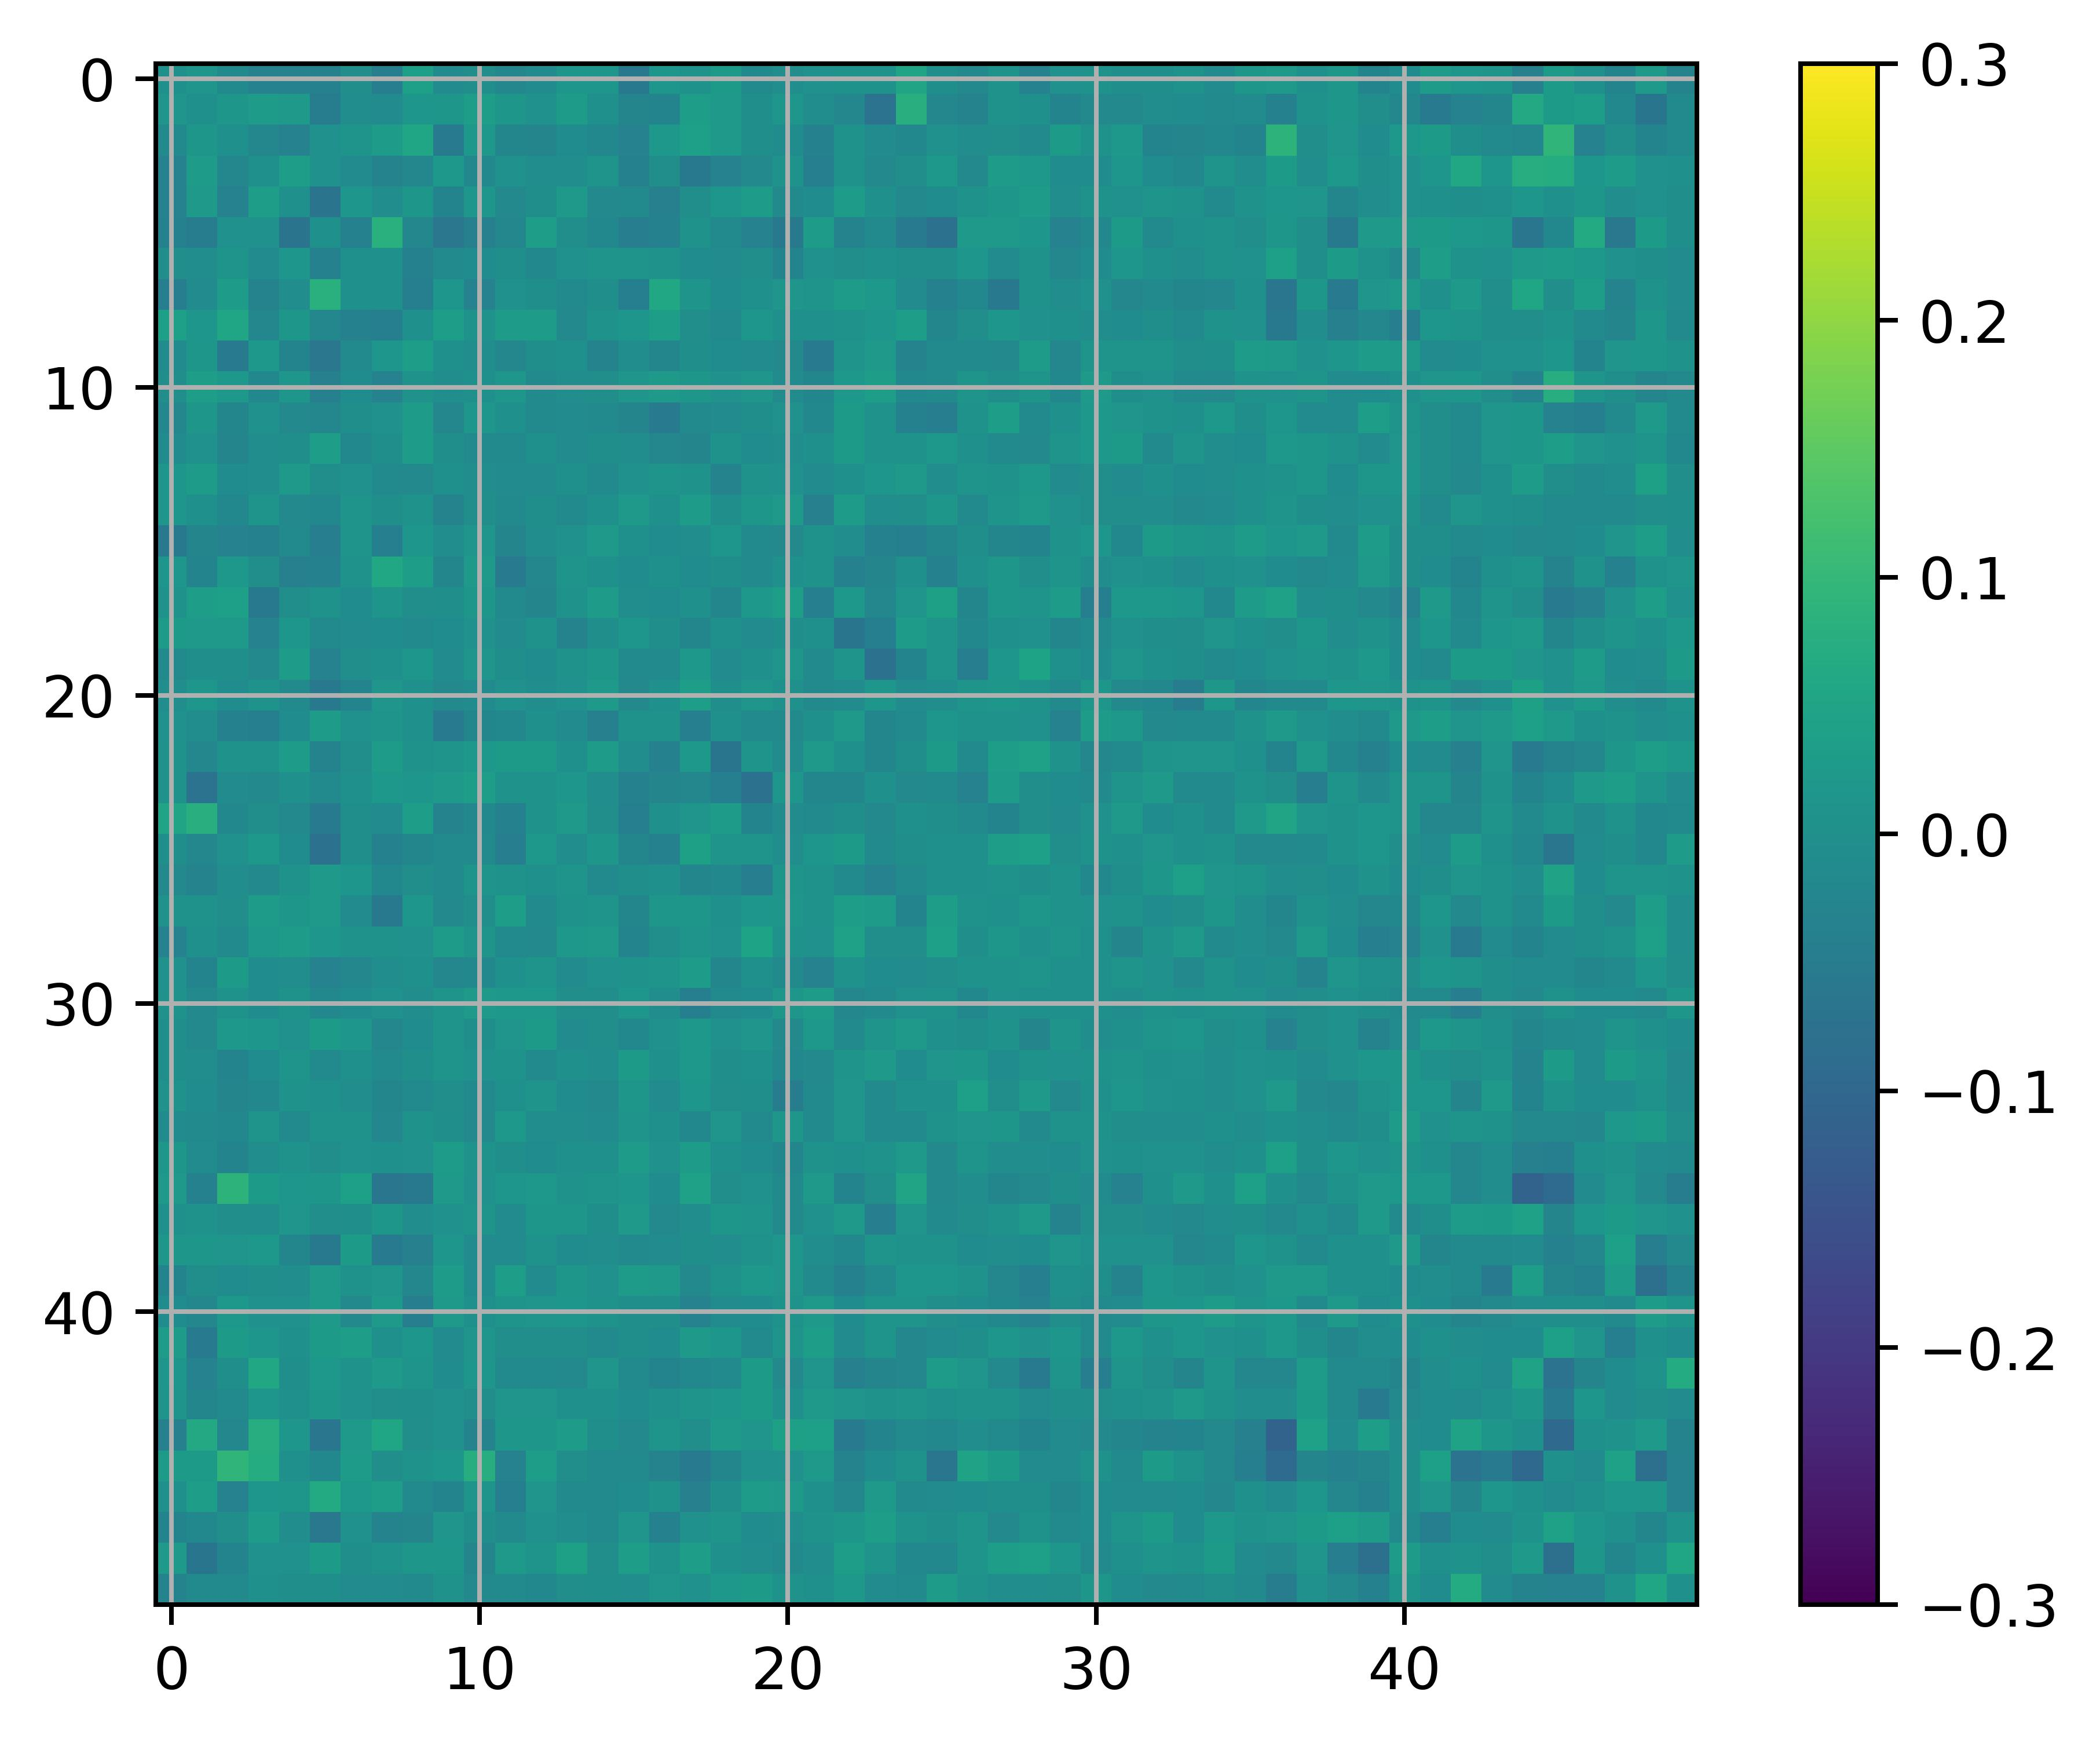
\includegraphics[width=0.2\textwidth]{../Analysis/DFC/size=480_step=180_rho=0.1/node=50_id=100206/c_10.jpg}
        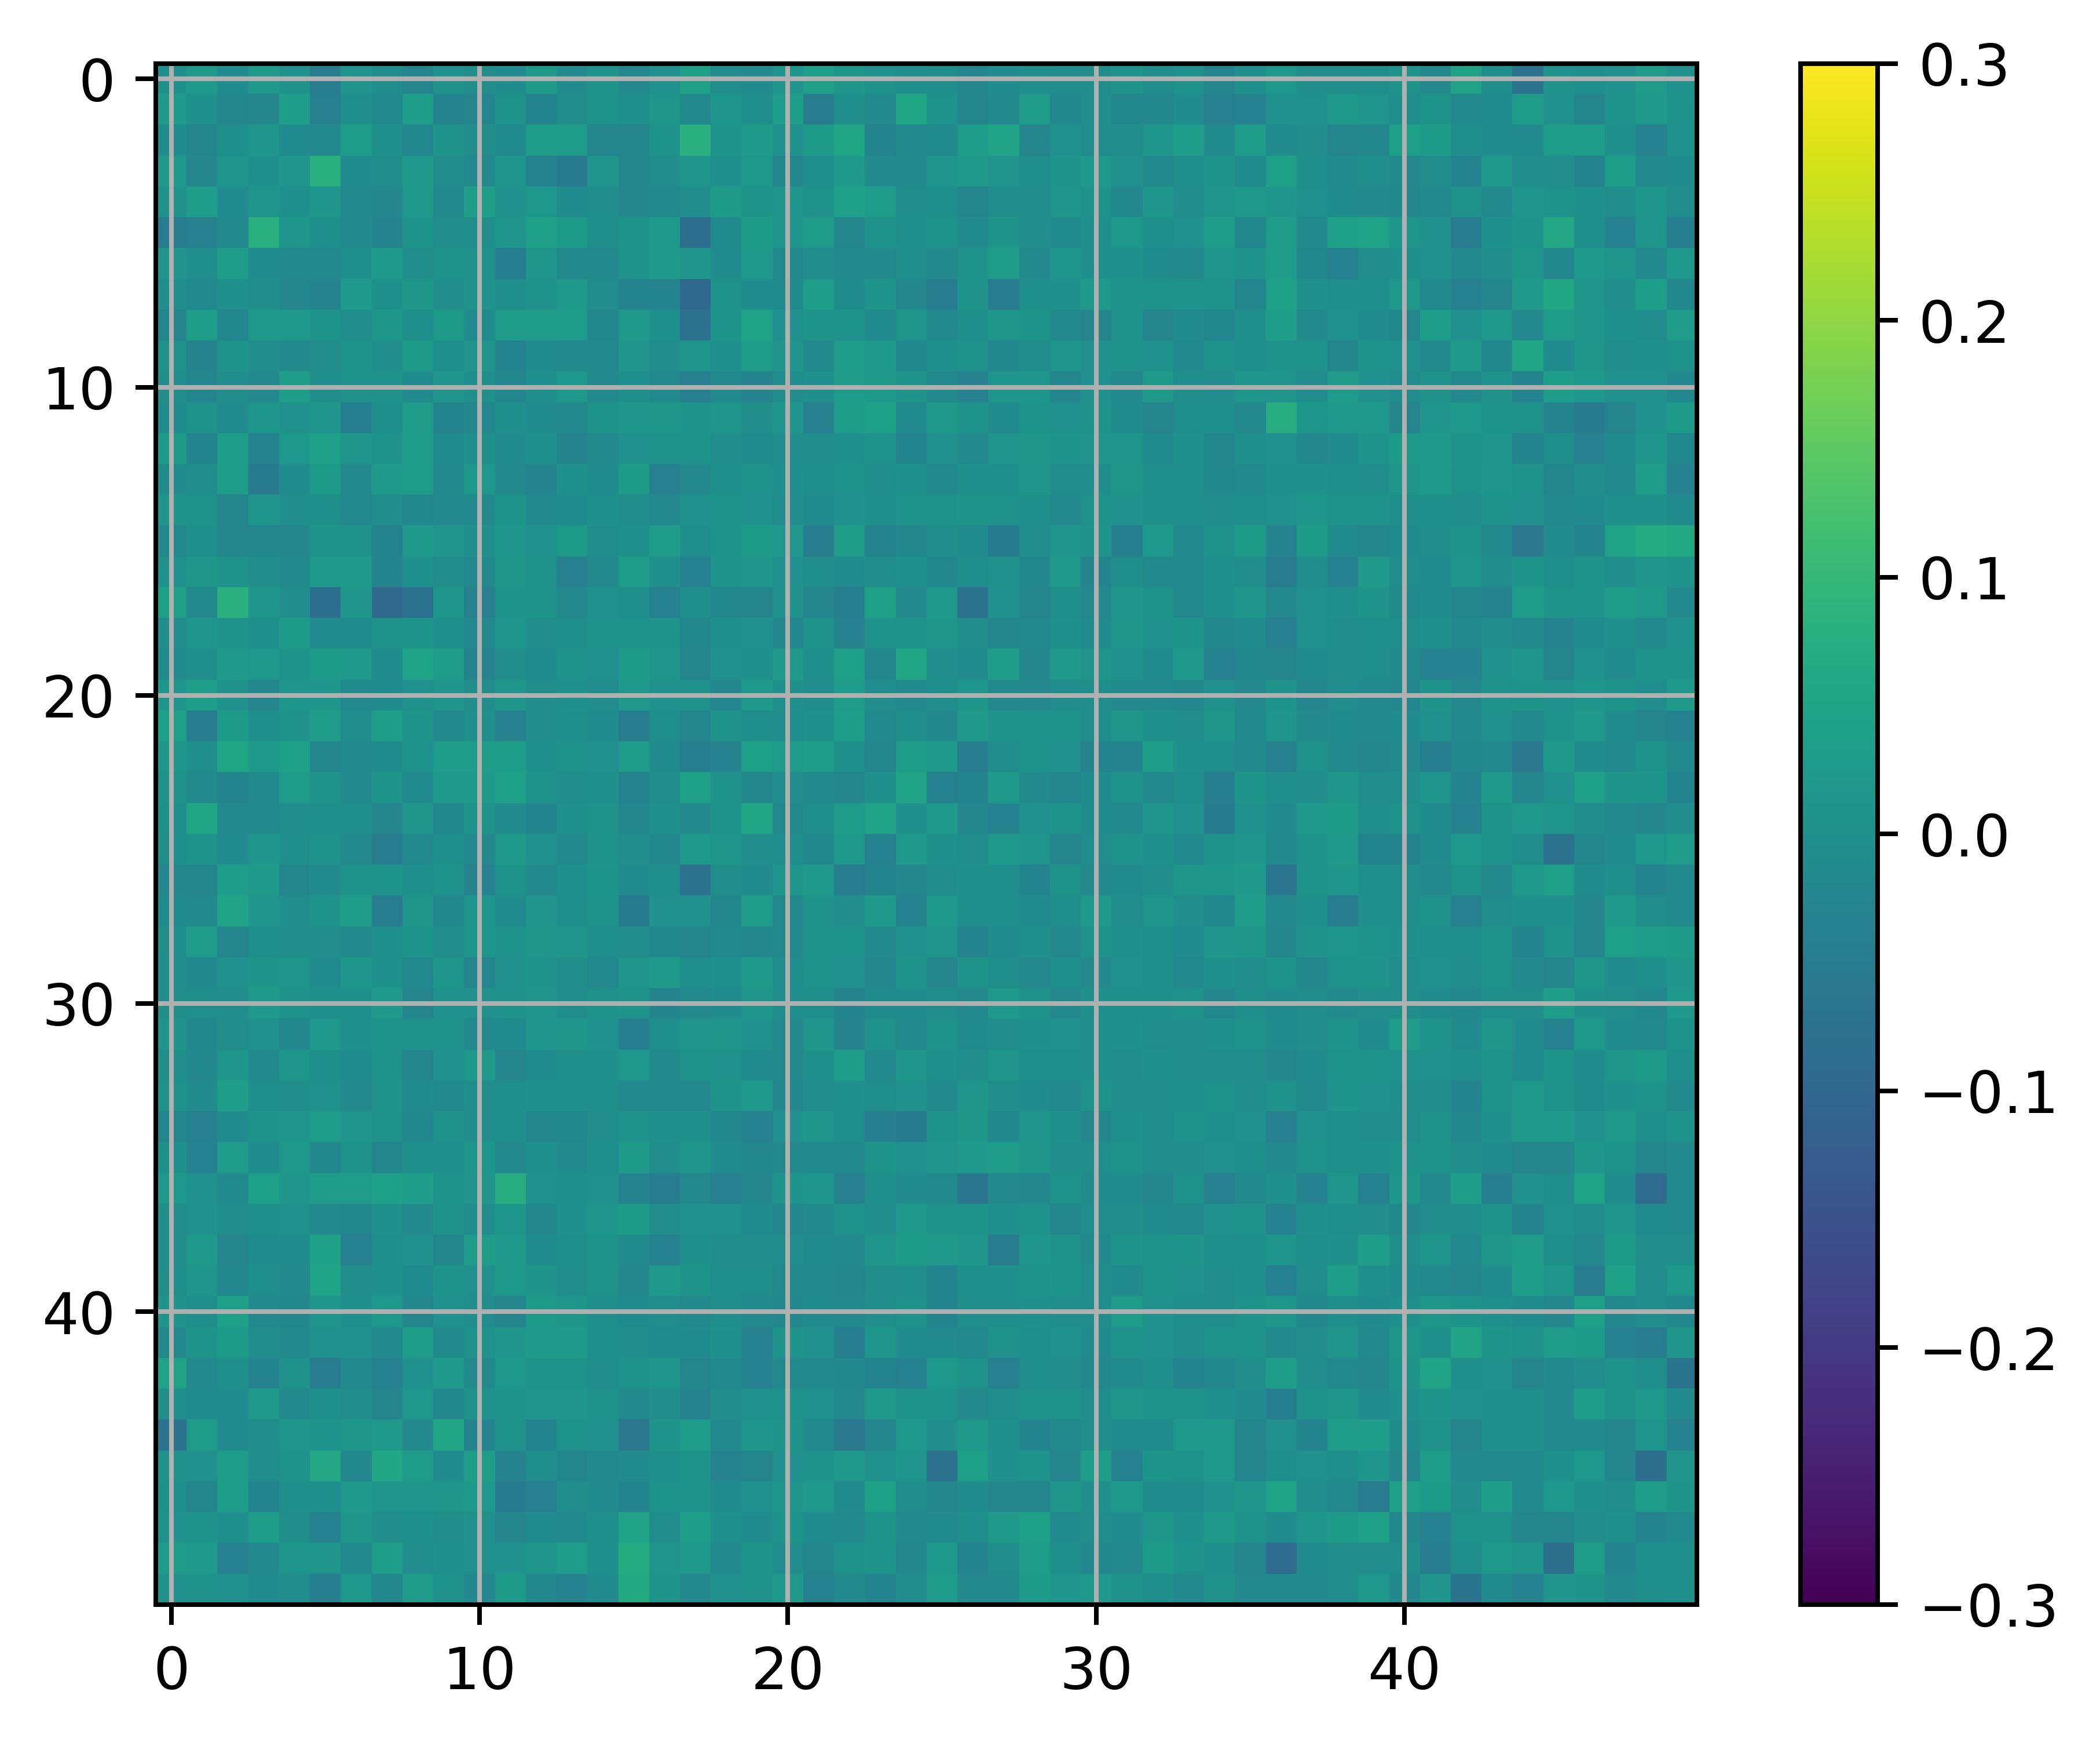
\includegraphics[width=0.2\textwidth]{../Analysis/DFC/size=480_step=180_rho=0.1/node=50_id=100206/c_12.jpg}
        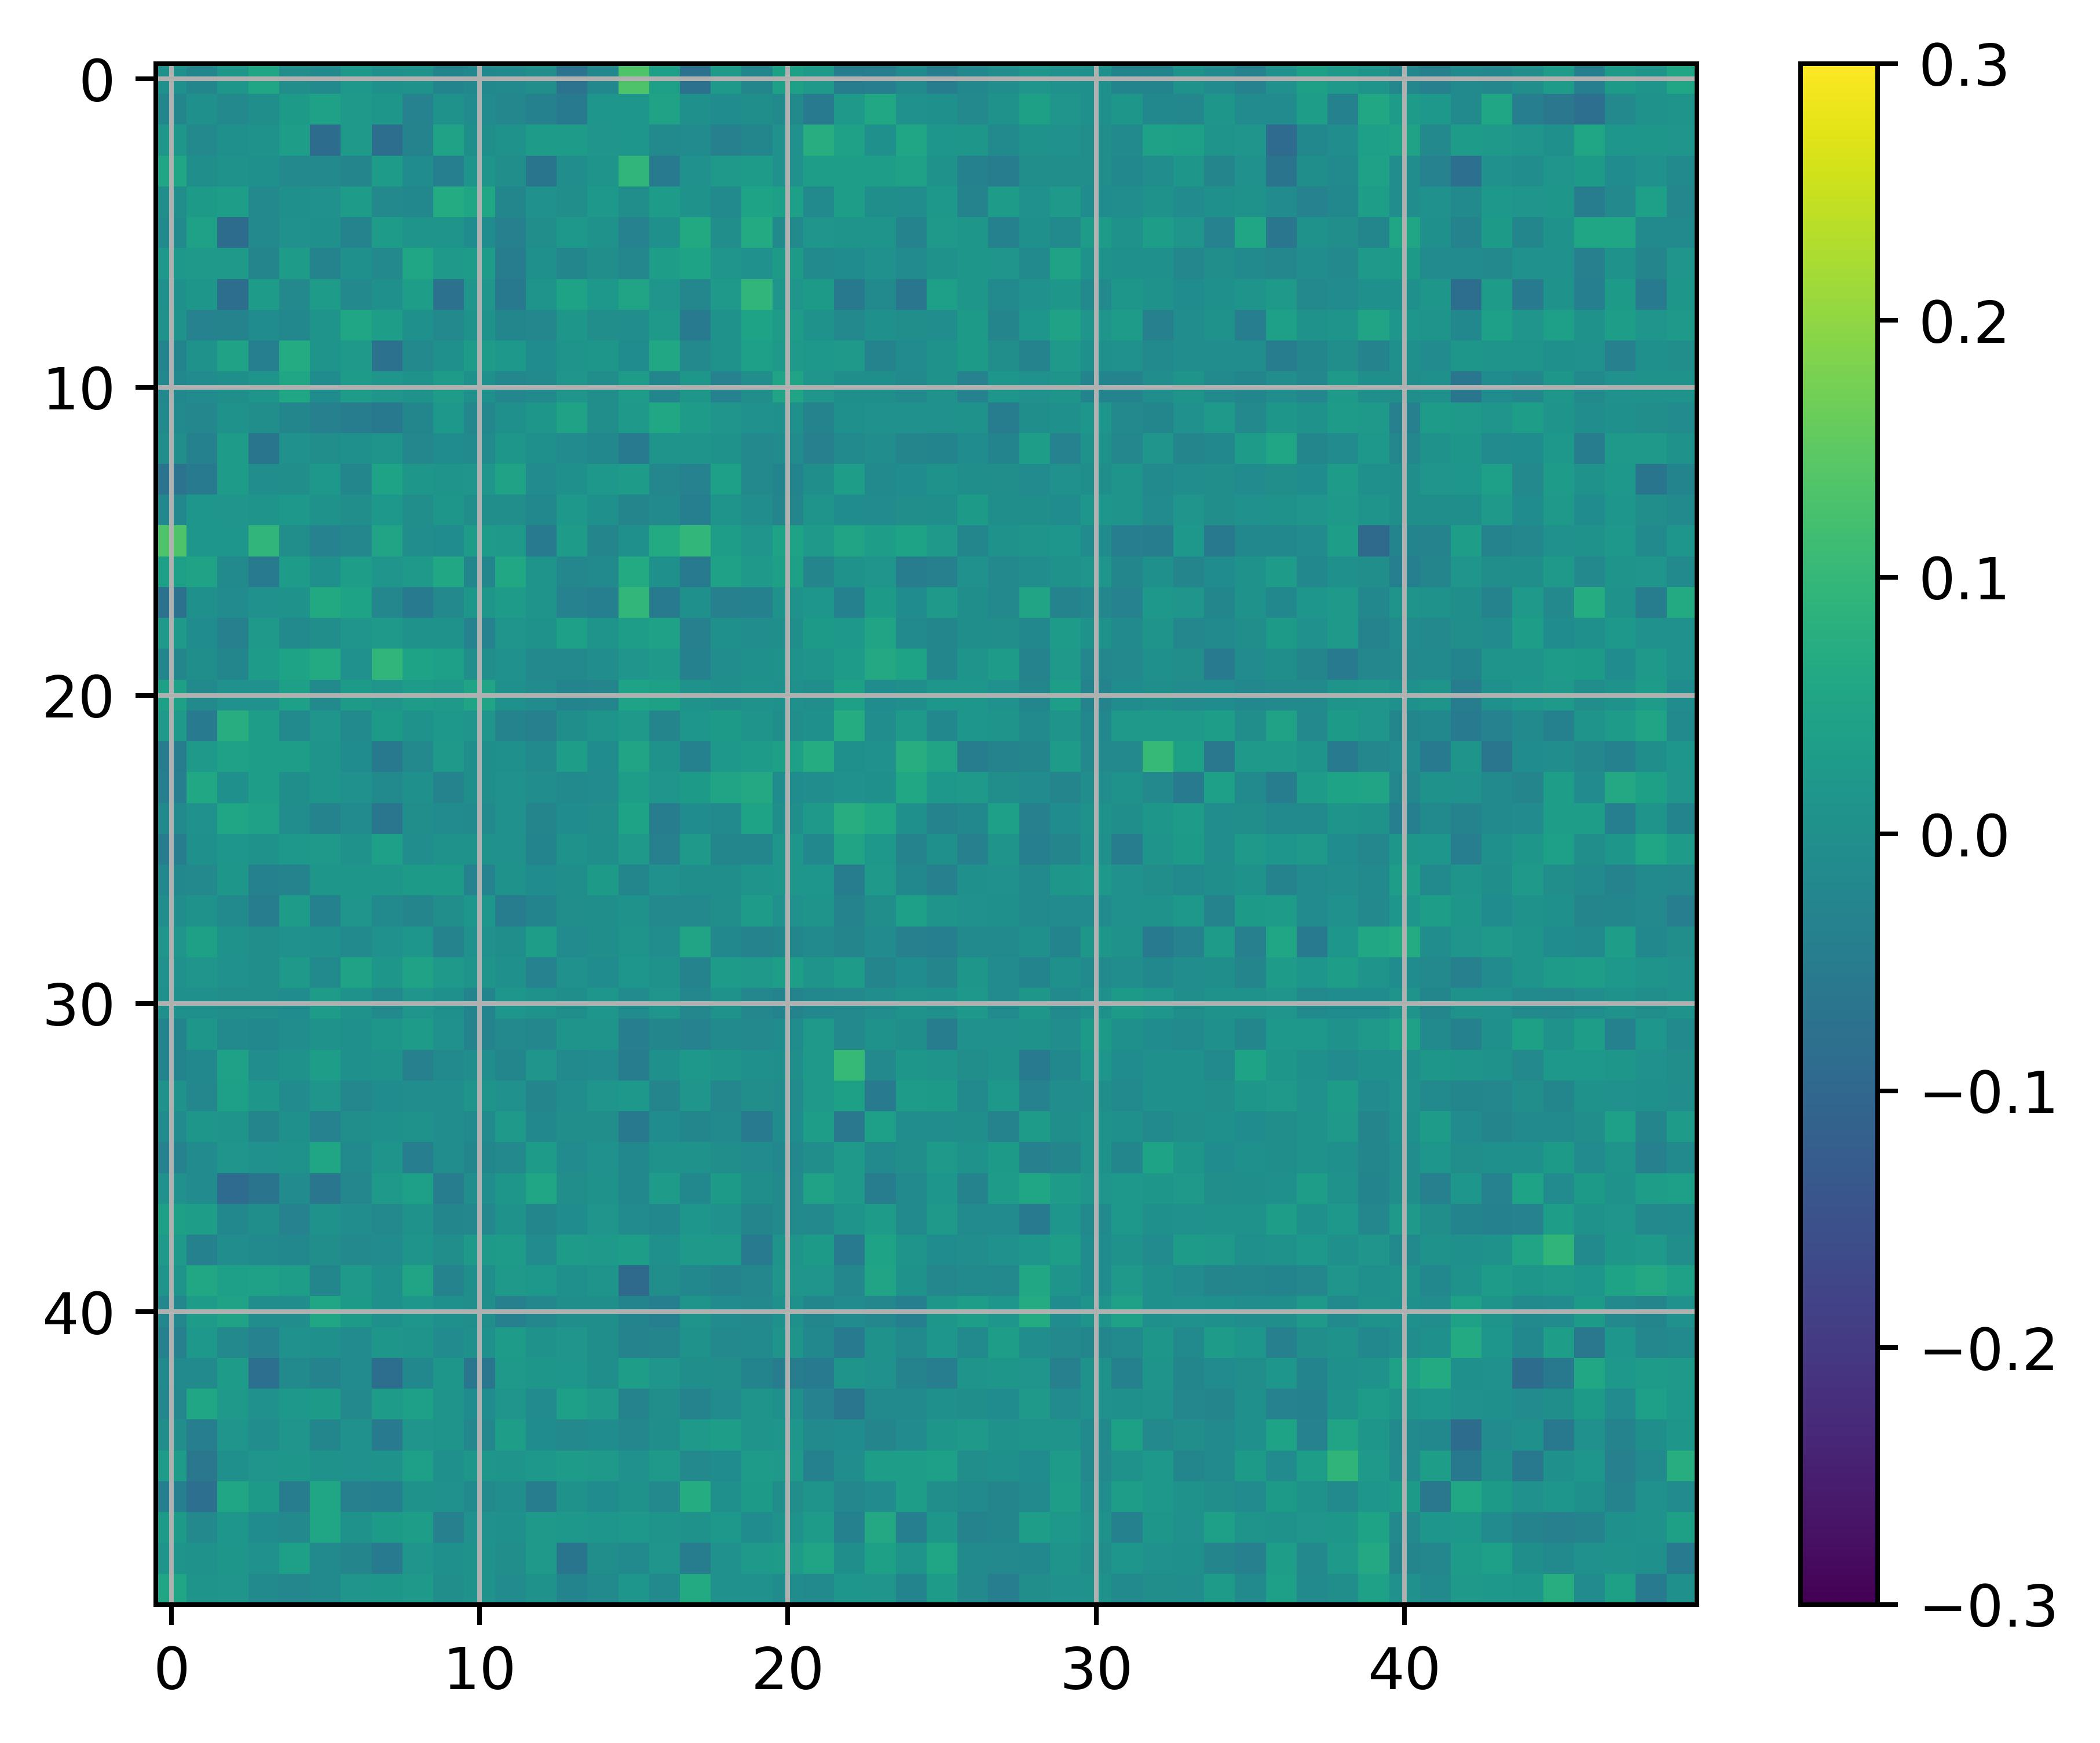
\includegraphics[width=0.2\textwidth]{../Analysis/DFC/size=480_step=180_rho=0.1/node=50_id=100206/c_14.jpg} \\
        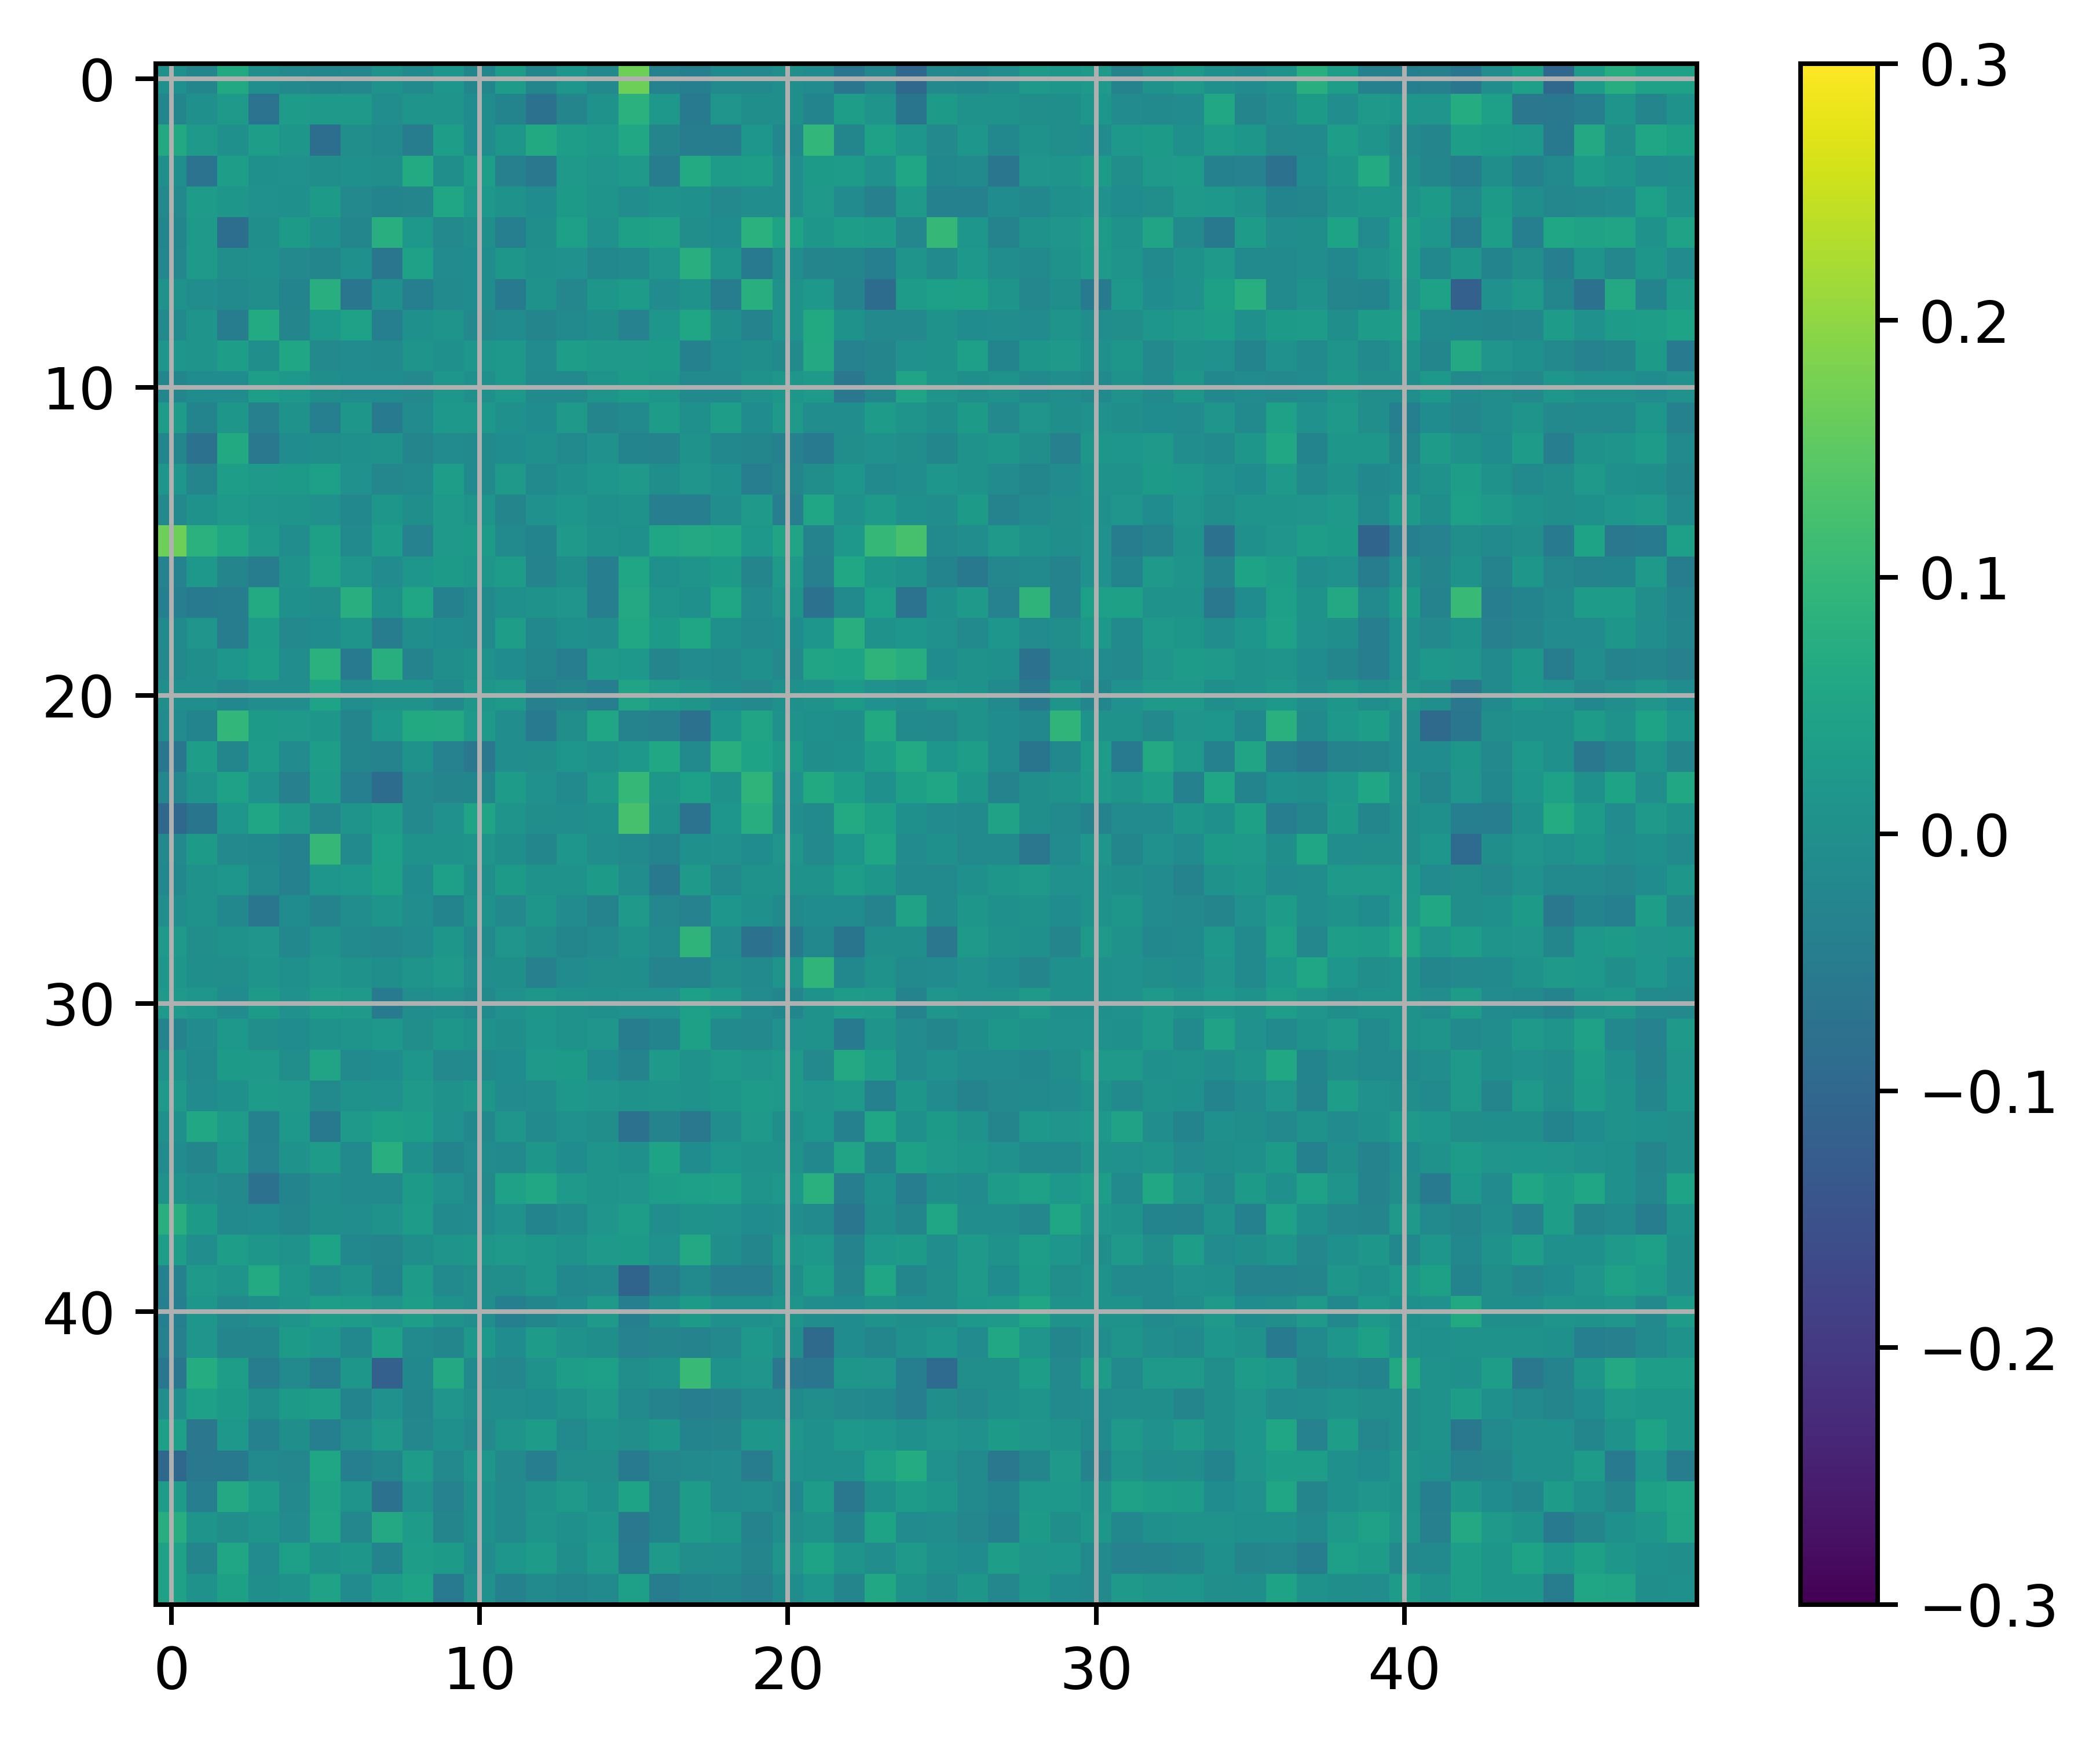
\includegraphics[width=0.2\textwidth]{../Analysis/DFC/size=480_step=180_rho=0.1/node=50_id=100206/c_16.jpg}
        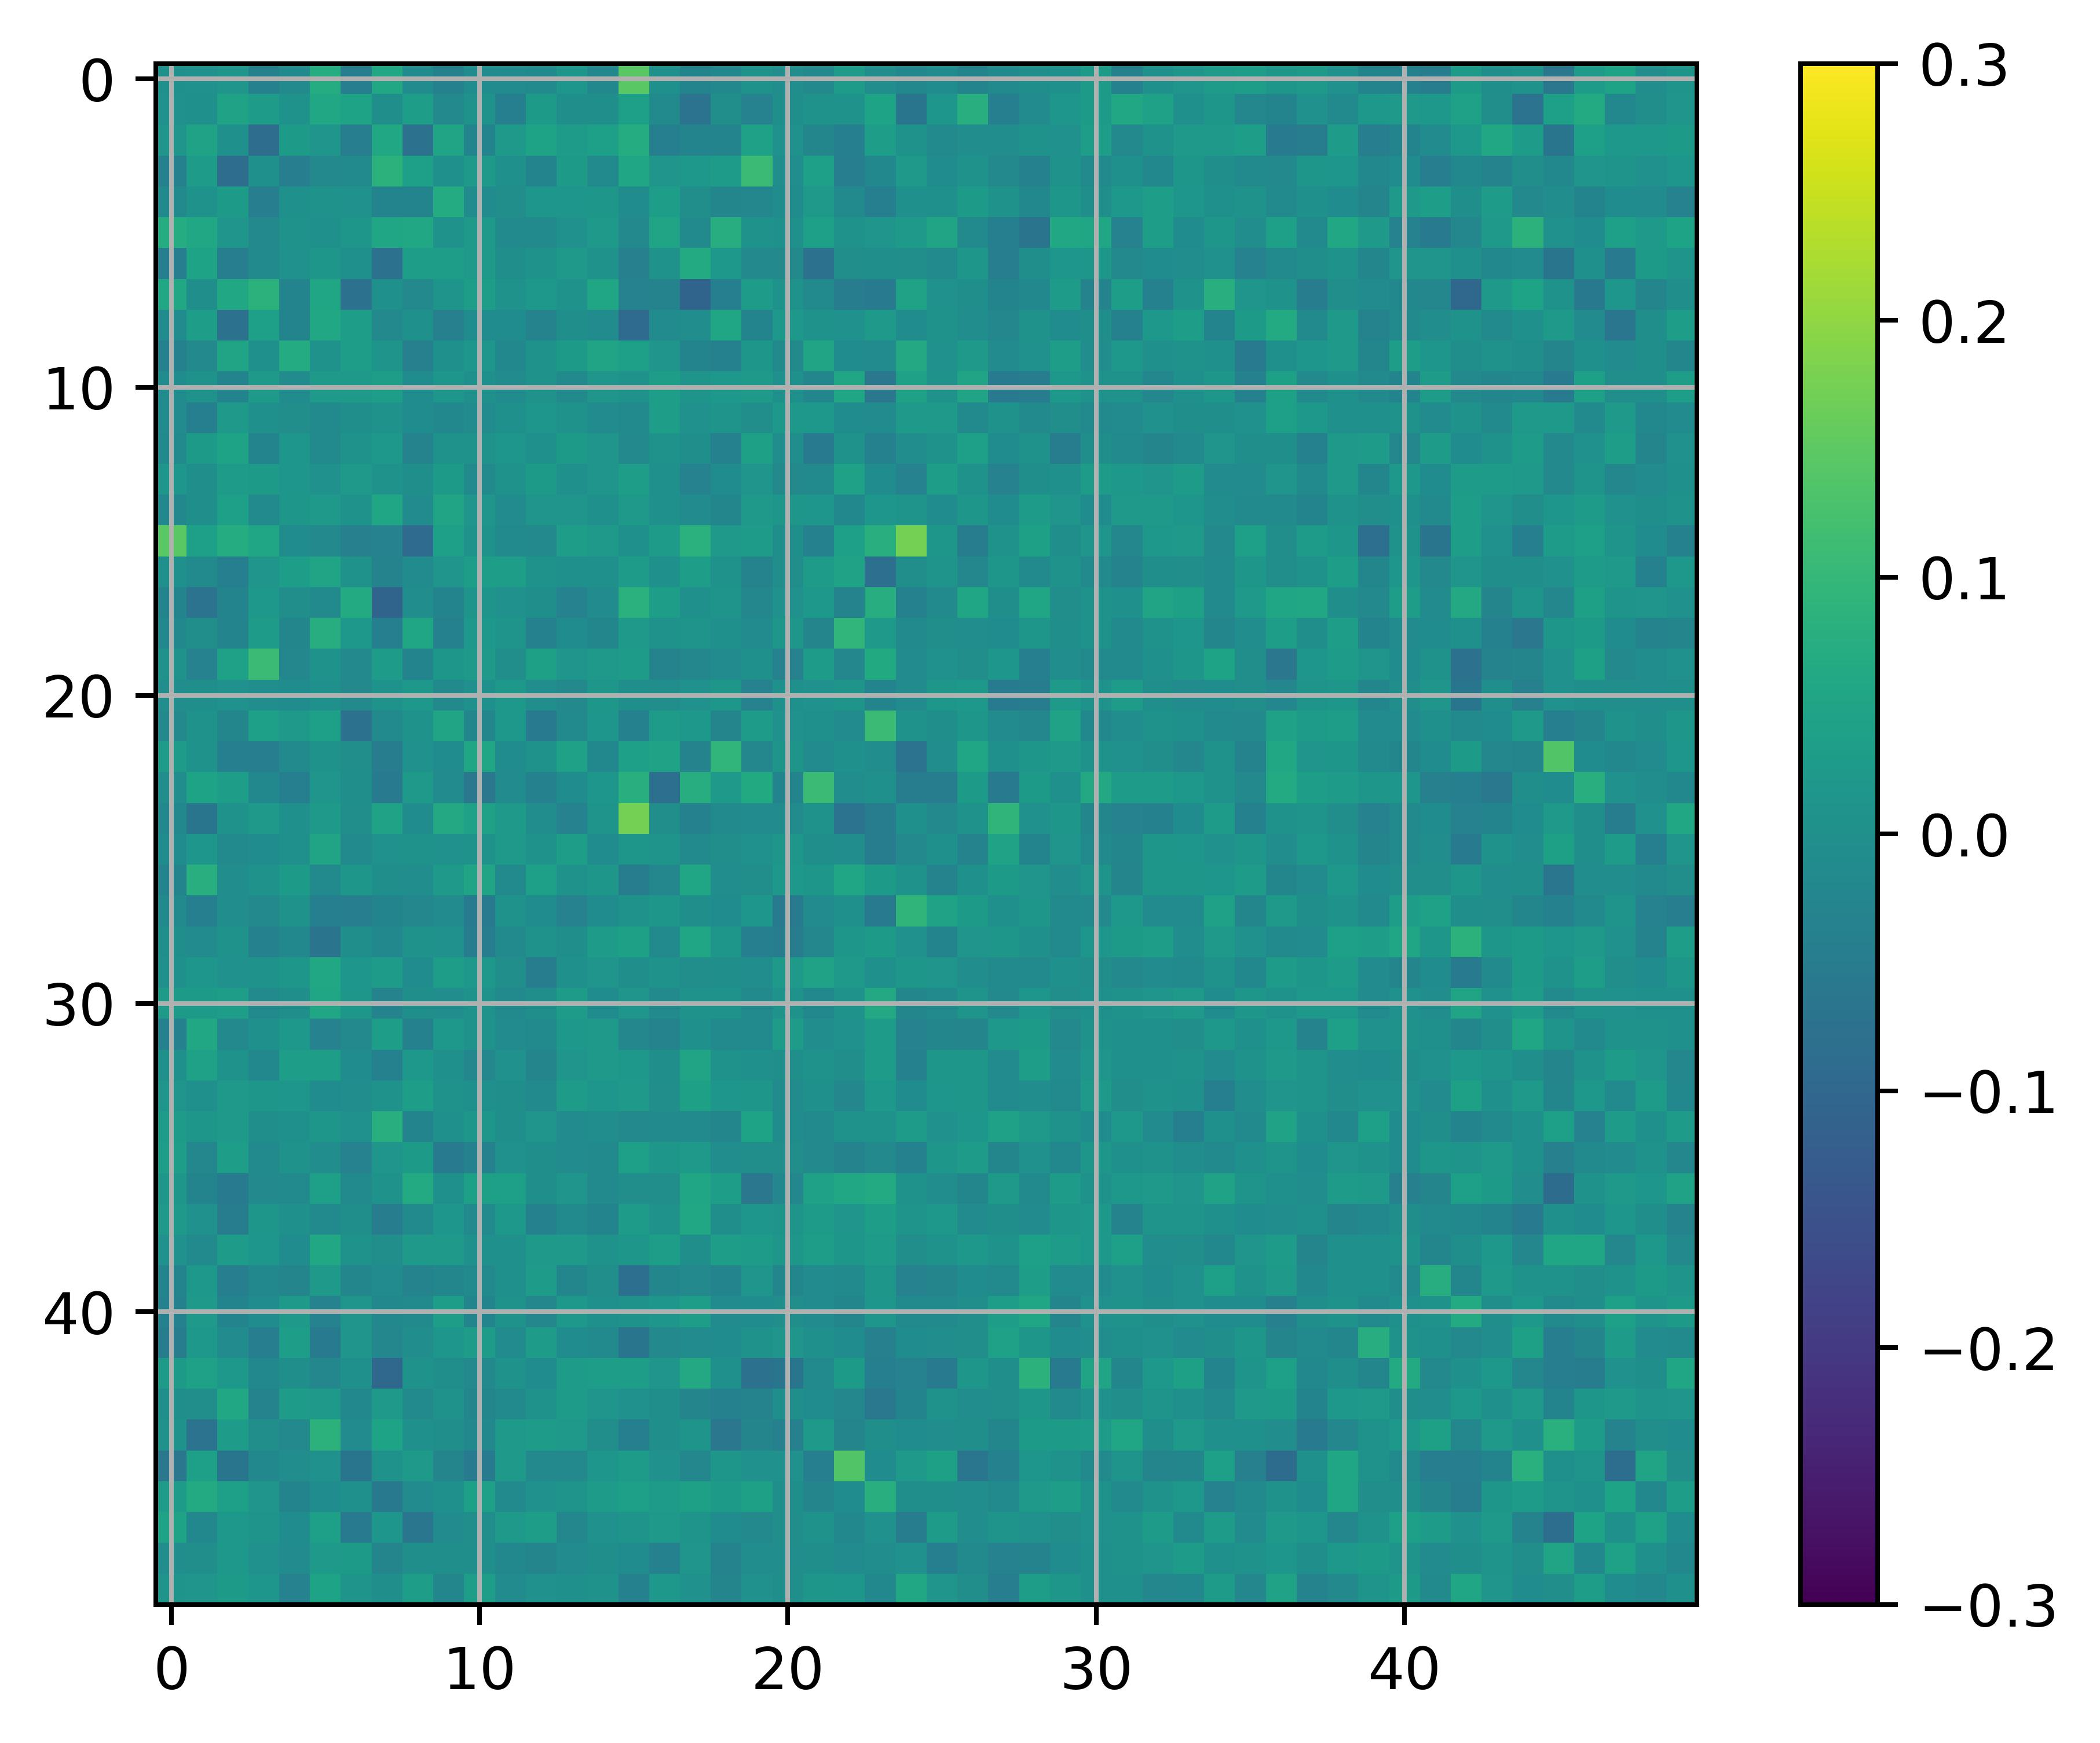
\includegraphics[width=0.2\textwidth]{../Analysis/DFC/size=480_step=180_rho=0.1/node=50_id=100206/c_18.jpg}
        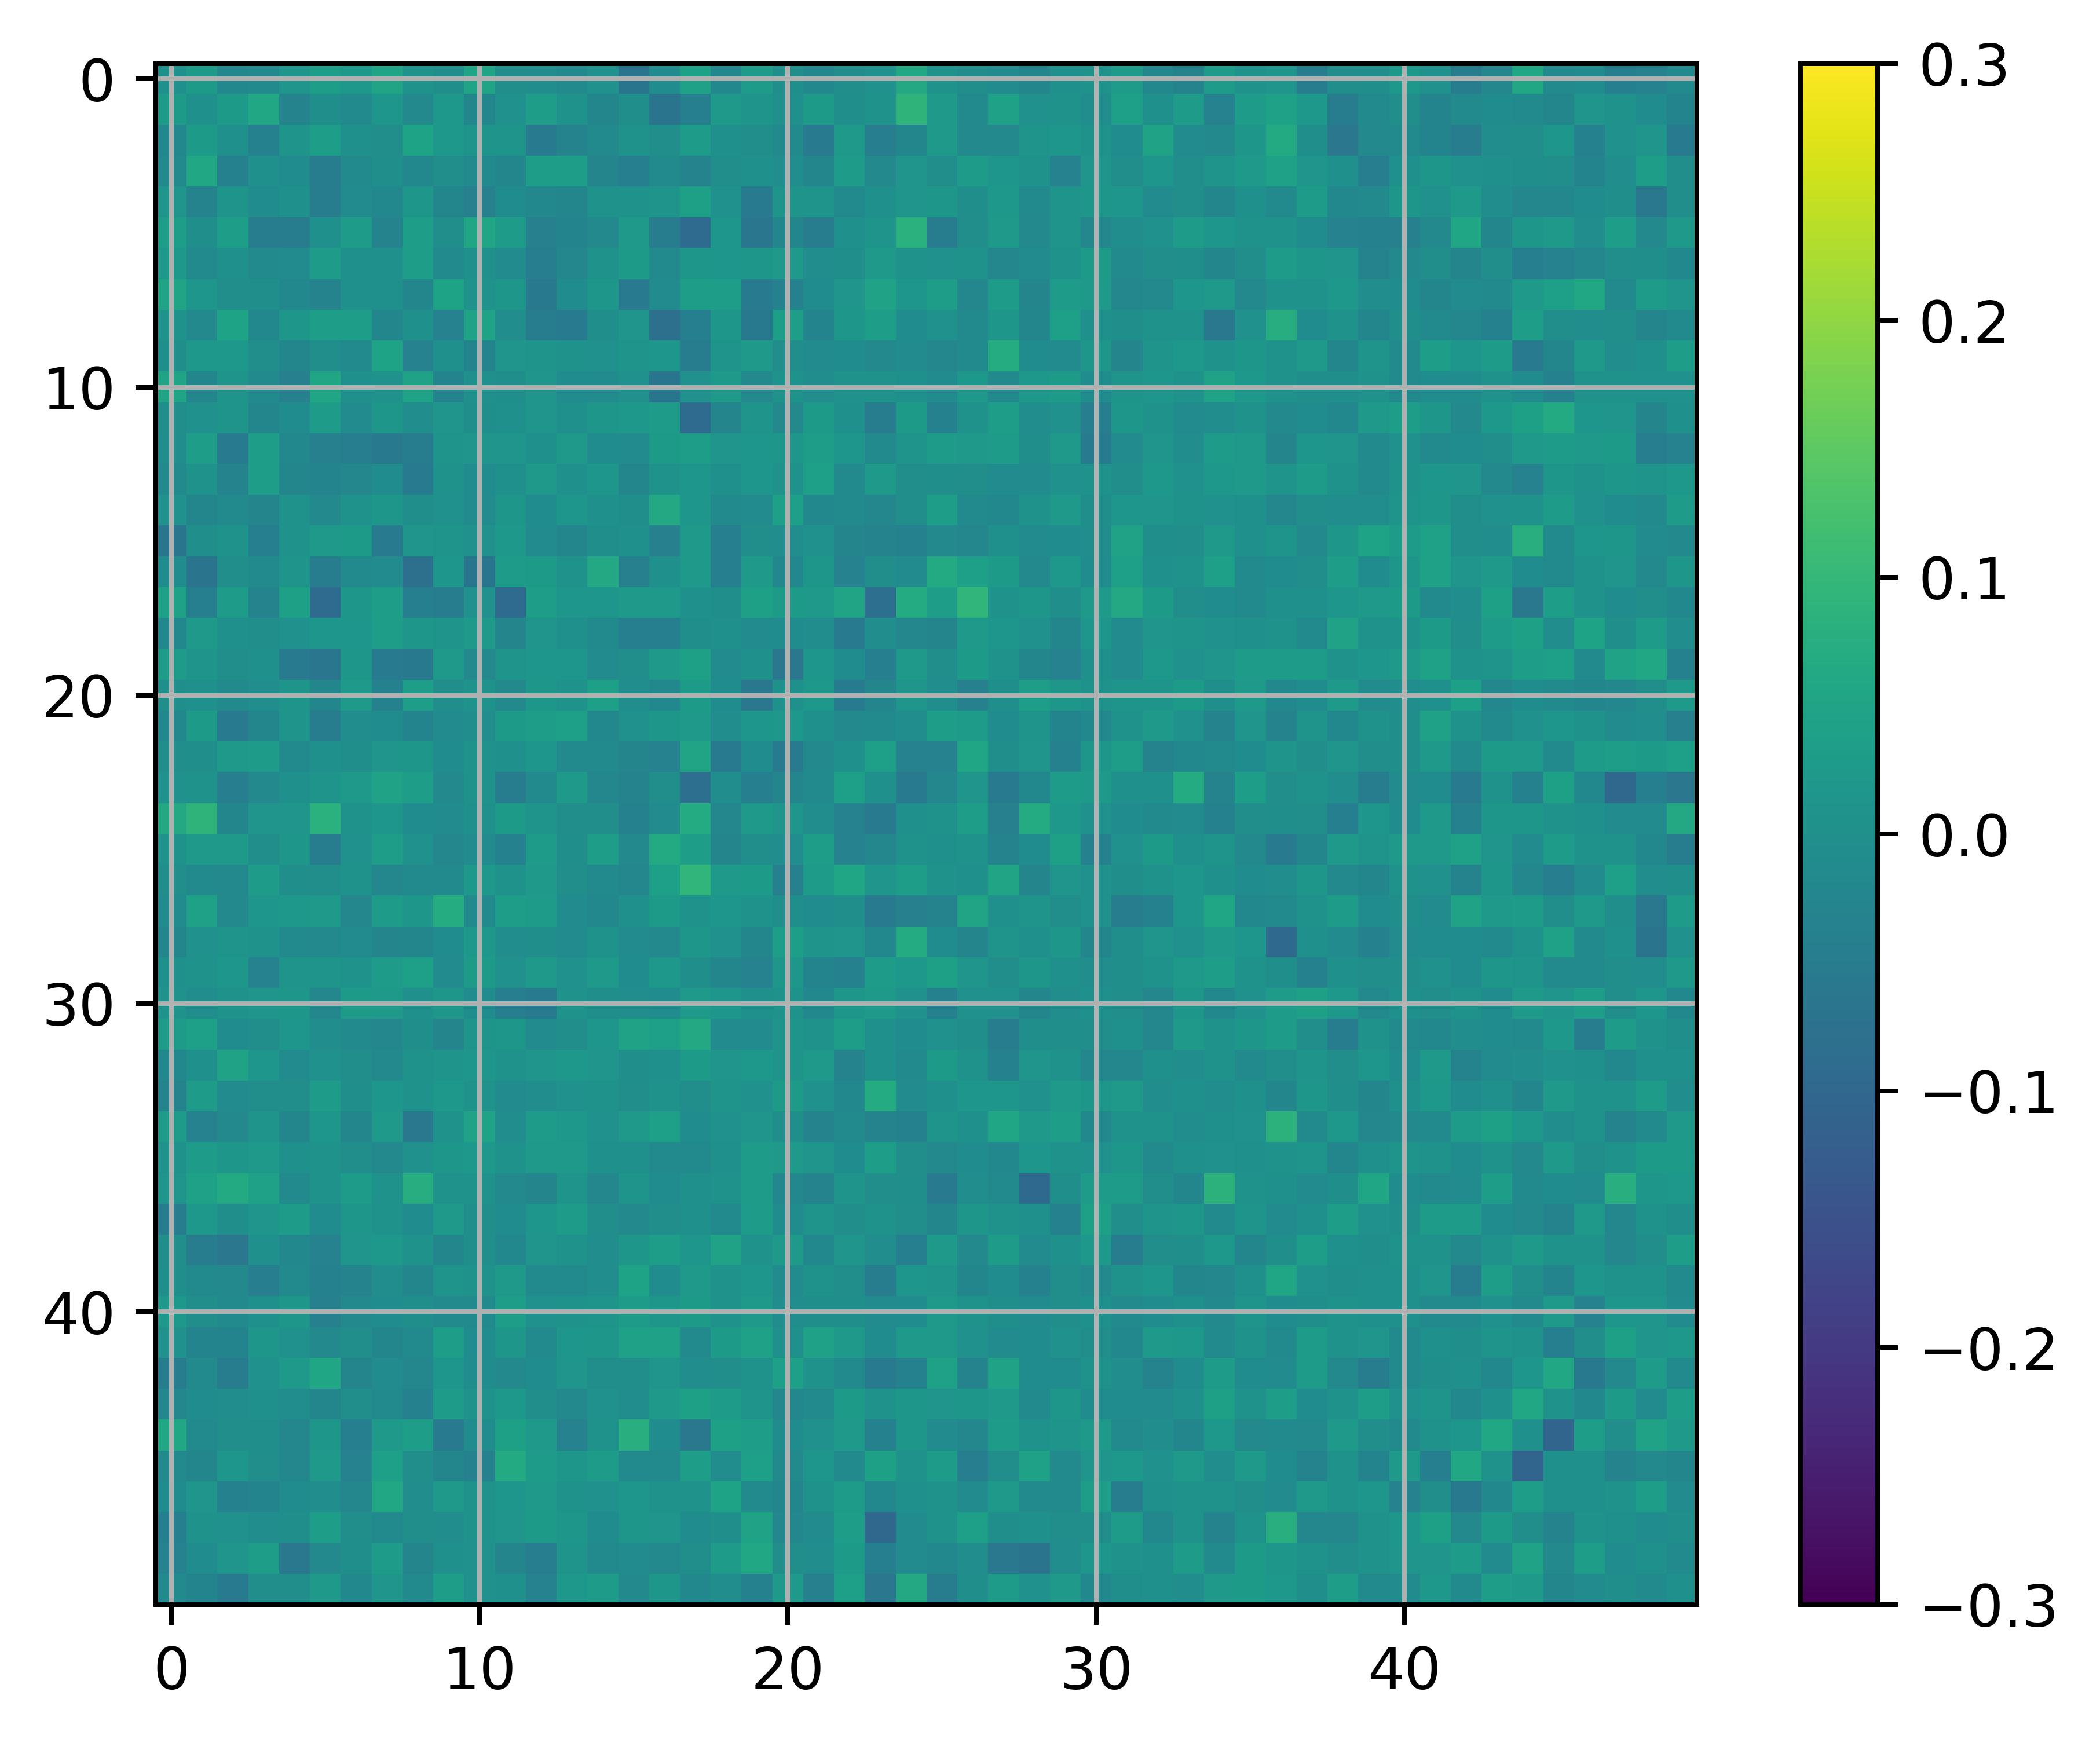
\includegraphics[width=0.2\textwidth]{../Analysis/DFC/size=480_step=180_rho=0.1/node=50_id=100206/c_20.jpg}
        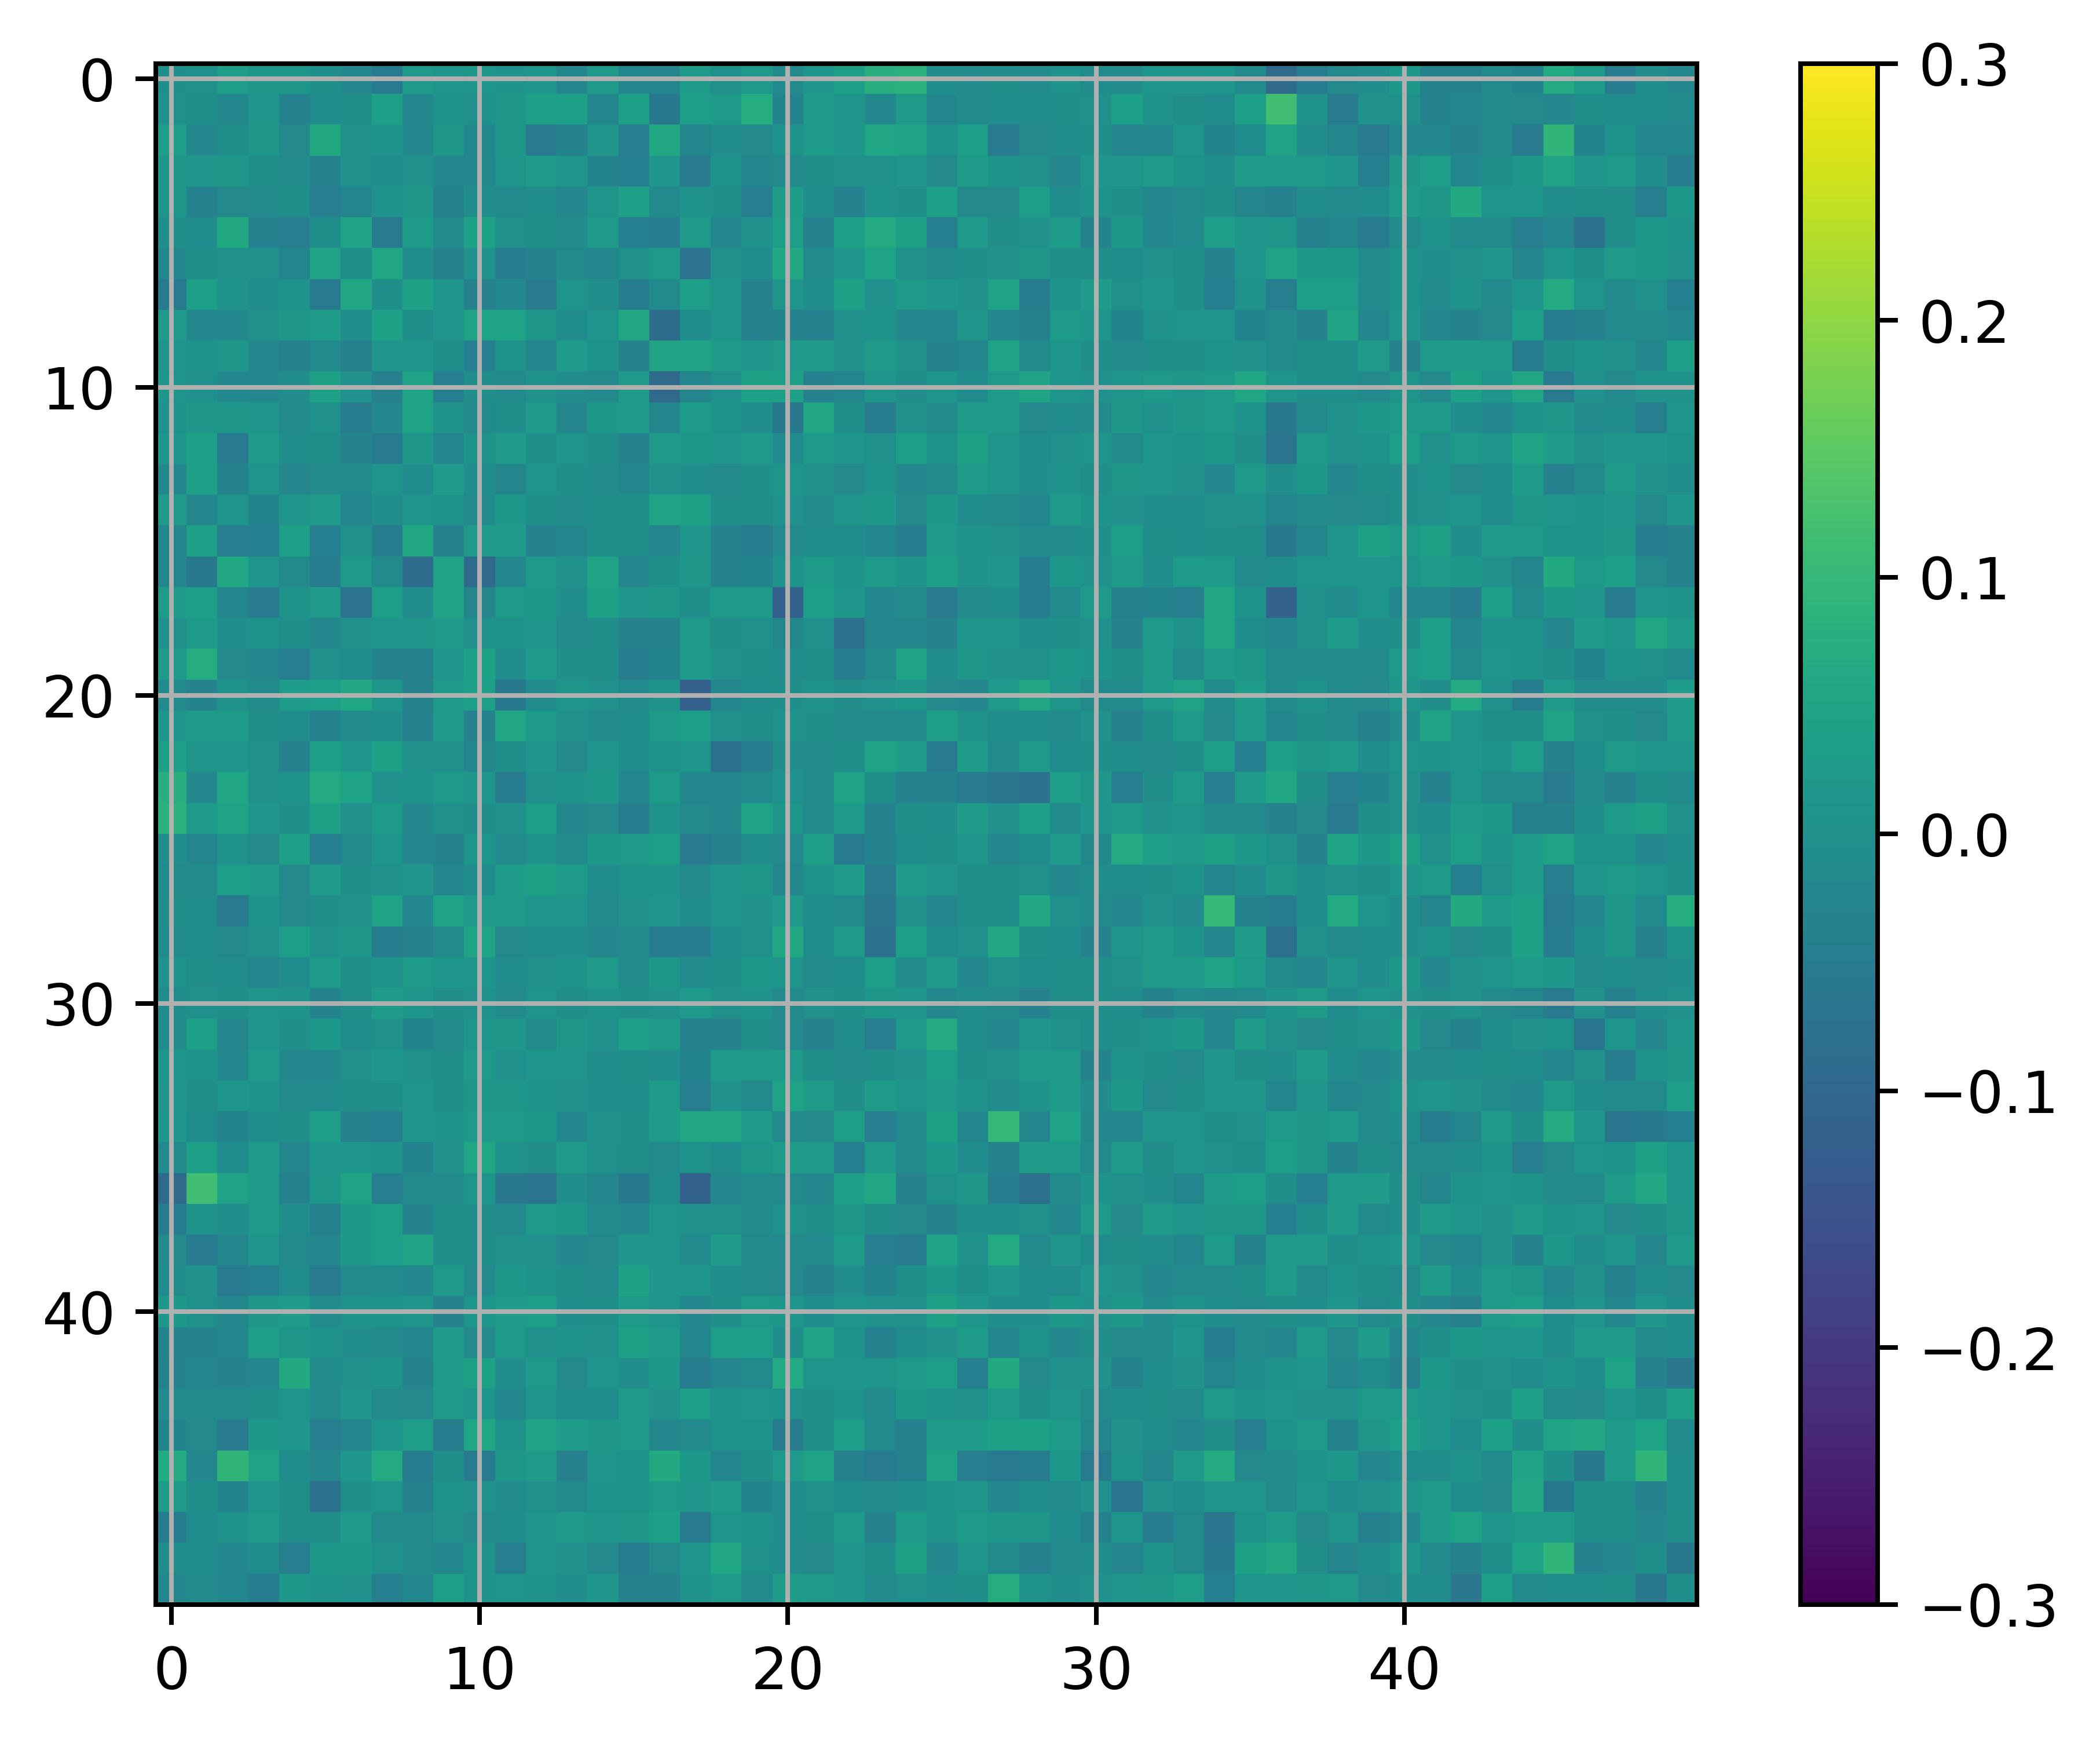
\includegraphics[width=0.2\textwidth]{../Analysis/DFC/size=480_step=180_rho=0.1/node=50_id=100206/c_22.jpg} \\
        \caption{Centered dynamic functional connectivity with $N_{node} = 50$.}
        % \label{LDA-example-1}
    \end{figure}

\end{frame}

\begin{frame}{Preprocessing - Examples}

    We compute the variance of each entry in dFC, which shows that the frames of dFC are more uniform with the increase of node.

    \begin{table}[H]
        \centering
        \begin{tabular}{|c|c|c|c|}
            \hline
            $N_{node}$ & min     & mean    & max     \\
            \hline
            $15$       & 5.76e-6 & 2.80e-5 & 1.99e-4 \\
            \hline
            $25$       & 2.82e-6 & 1.07e-5 & 6.07e-5 \\
            \hline
            $50$       & 1.63e-8 & 1.34e-6 & 4.90e-6 \\
            \hline
        \end{tabular}
        % \label{table1}
        \caption{Variance of dFC}
    \end{table}

\end{frame}

% \begin{frame}{Method}

%     With a fixed number of training samples, the predictive power reduces as the number of predictor variables increases\footfullcite{Hughes1968-ga}.

% \end{frame}

\begin{frame}{SVM\footfullcite{Vapnik1997-yy}\footfullcite{Cortes1995-dg}}

    Given a dataset $\{ (\mathbf{x}_i, y_i) \}_{i=1}^N$, a linear SVM aims to find a vector $\mathbf{w}$ and a number $b$ such that the data can be separated via the distance $\mathbf{w}^T \mathbf{x}_i - b$.

    \begin{figure}[H]
        \centering
        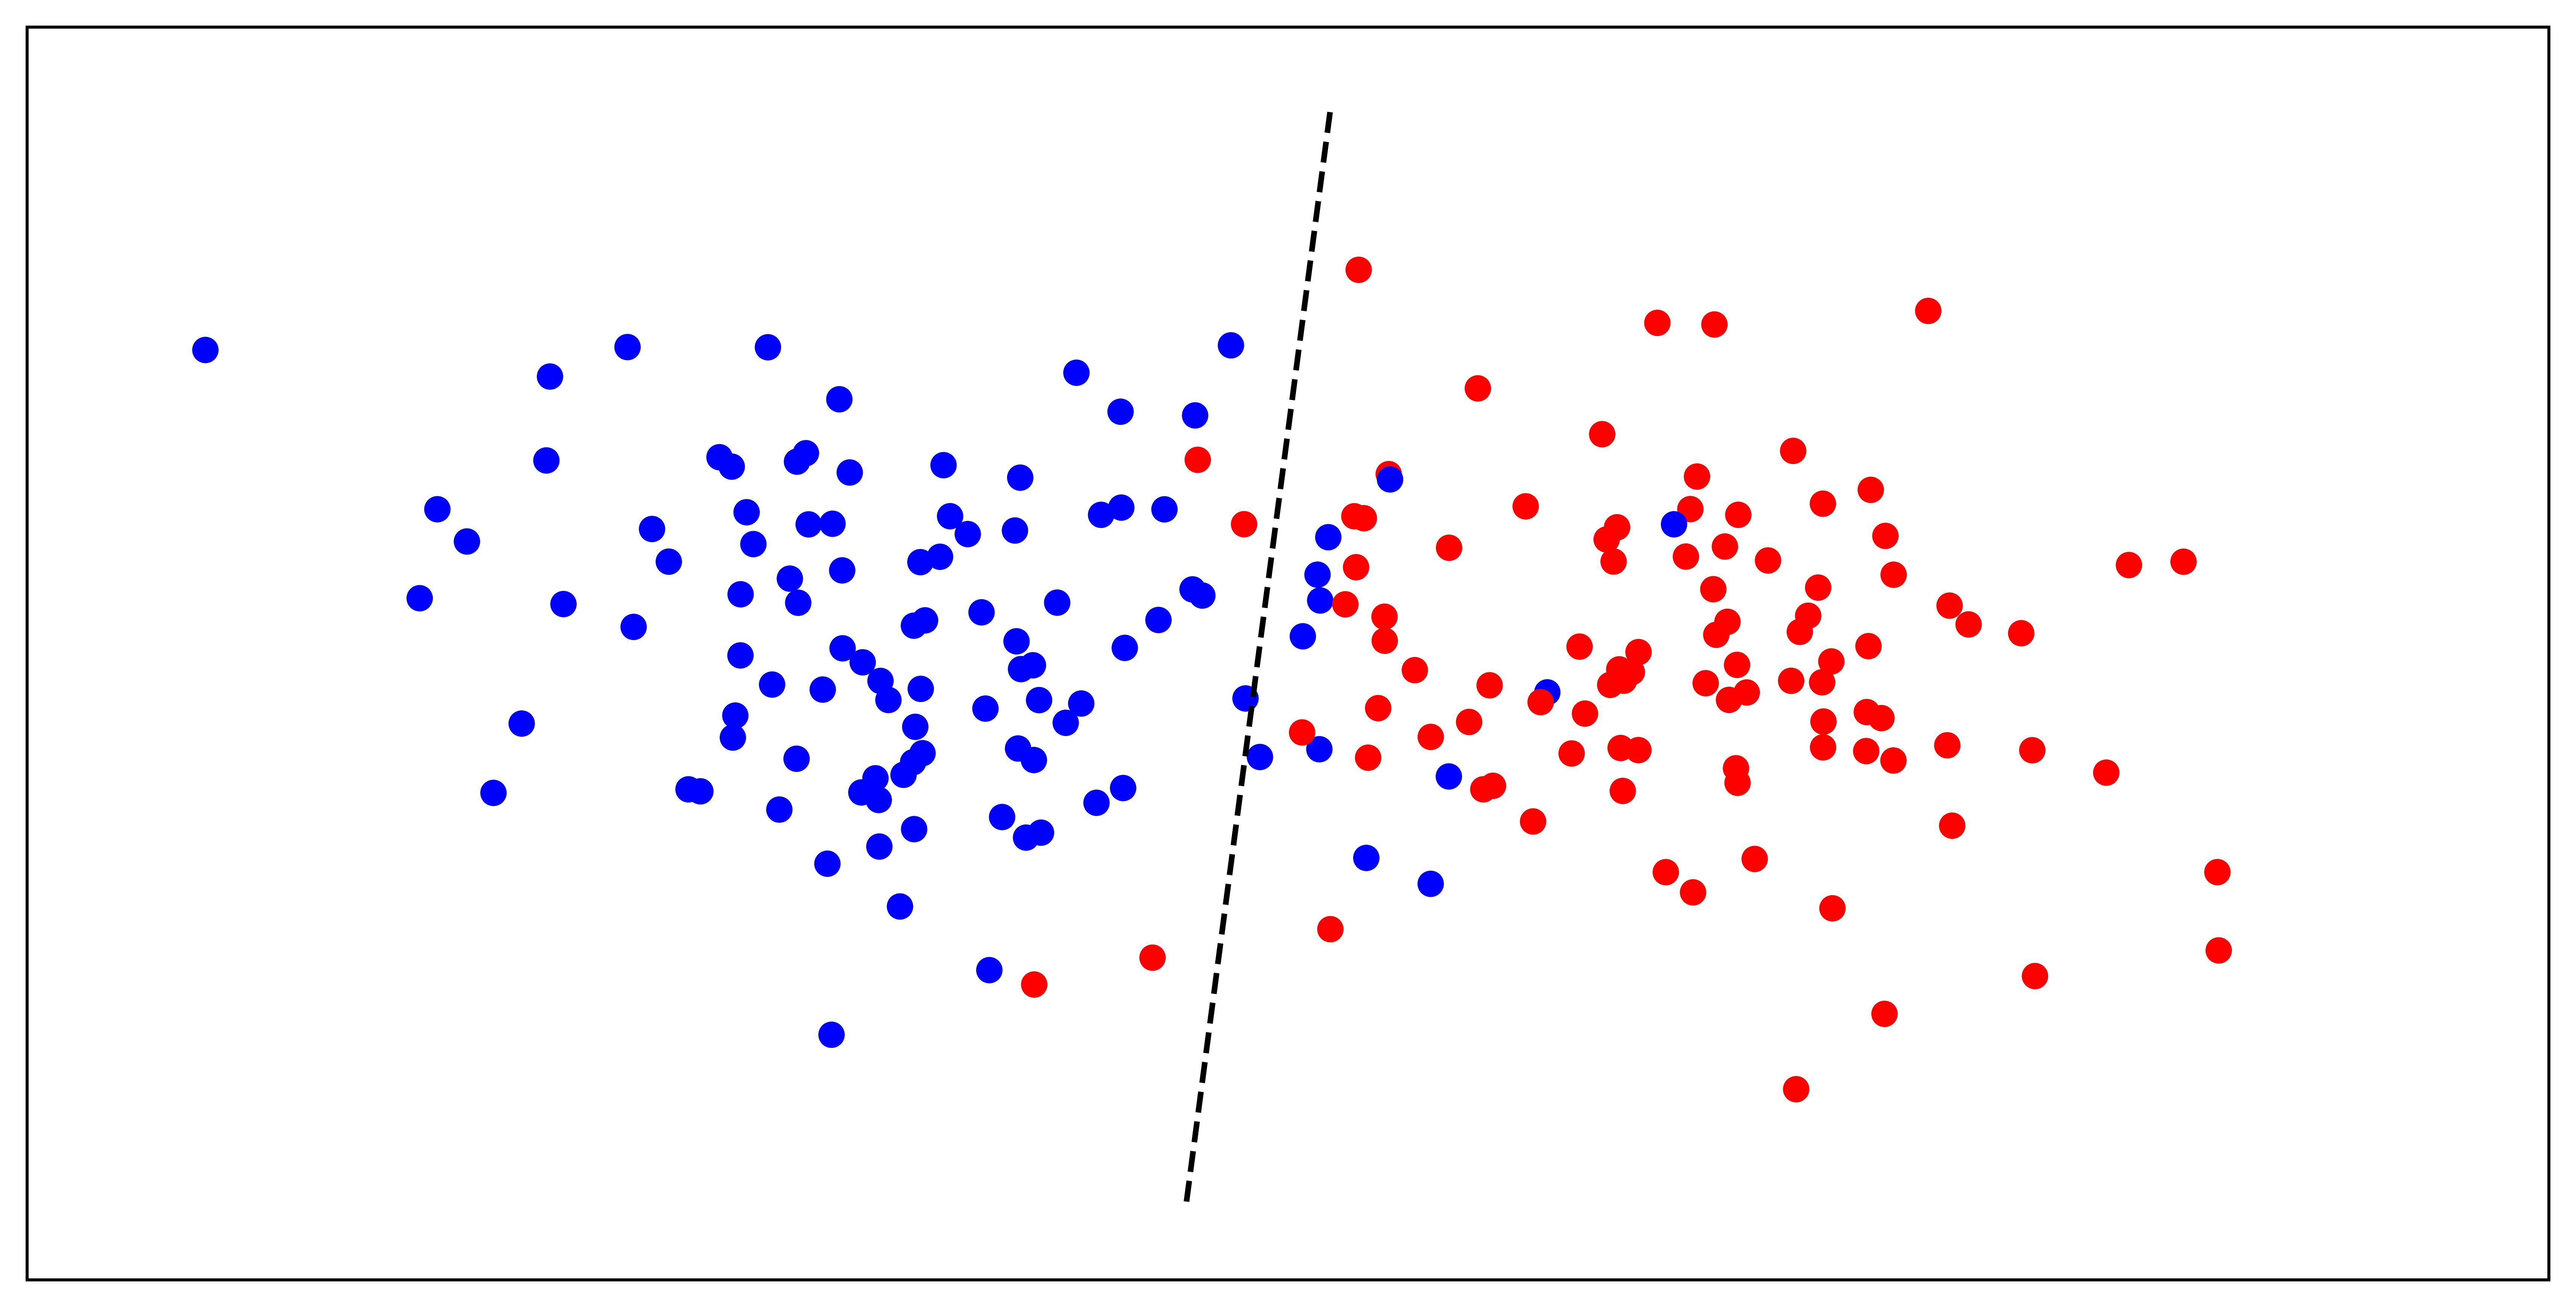
\includegraphics[width=0.6\textwidth]{./figure/svm.jpg}
    \end{figure}

\end{frame}

\begin{frame}{SVM - Results}

    \begin{figure}[H]
        \centering
        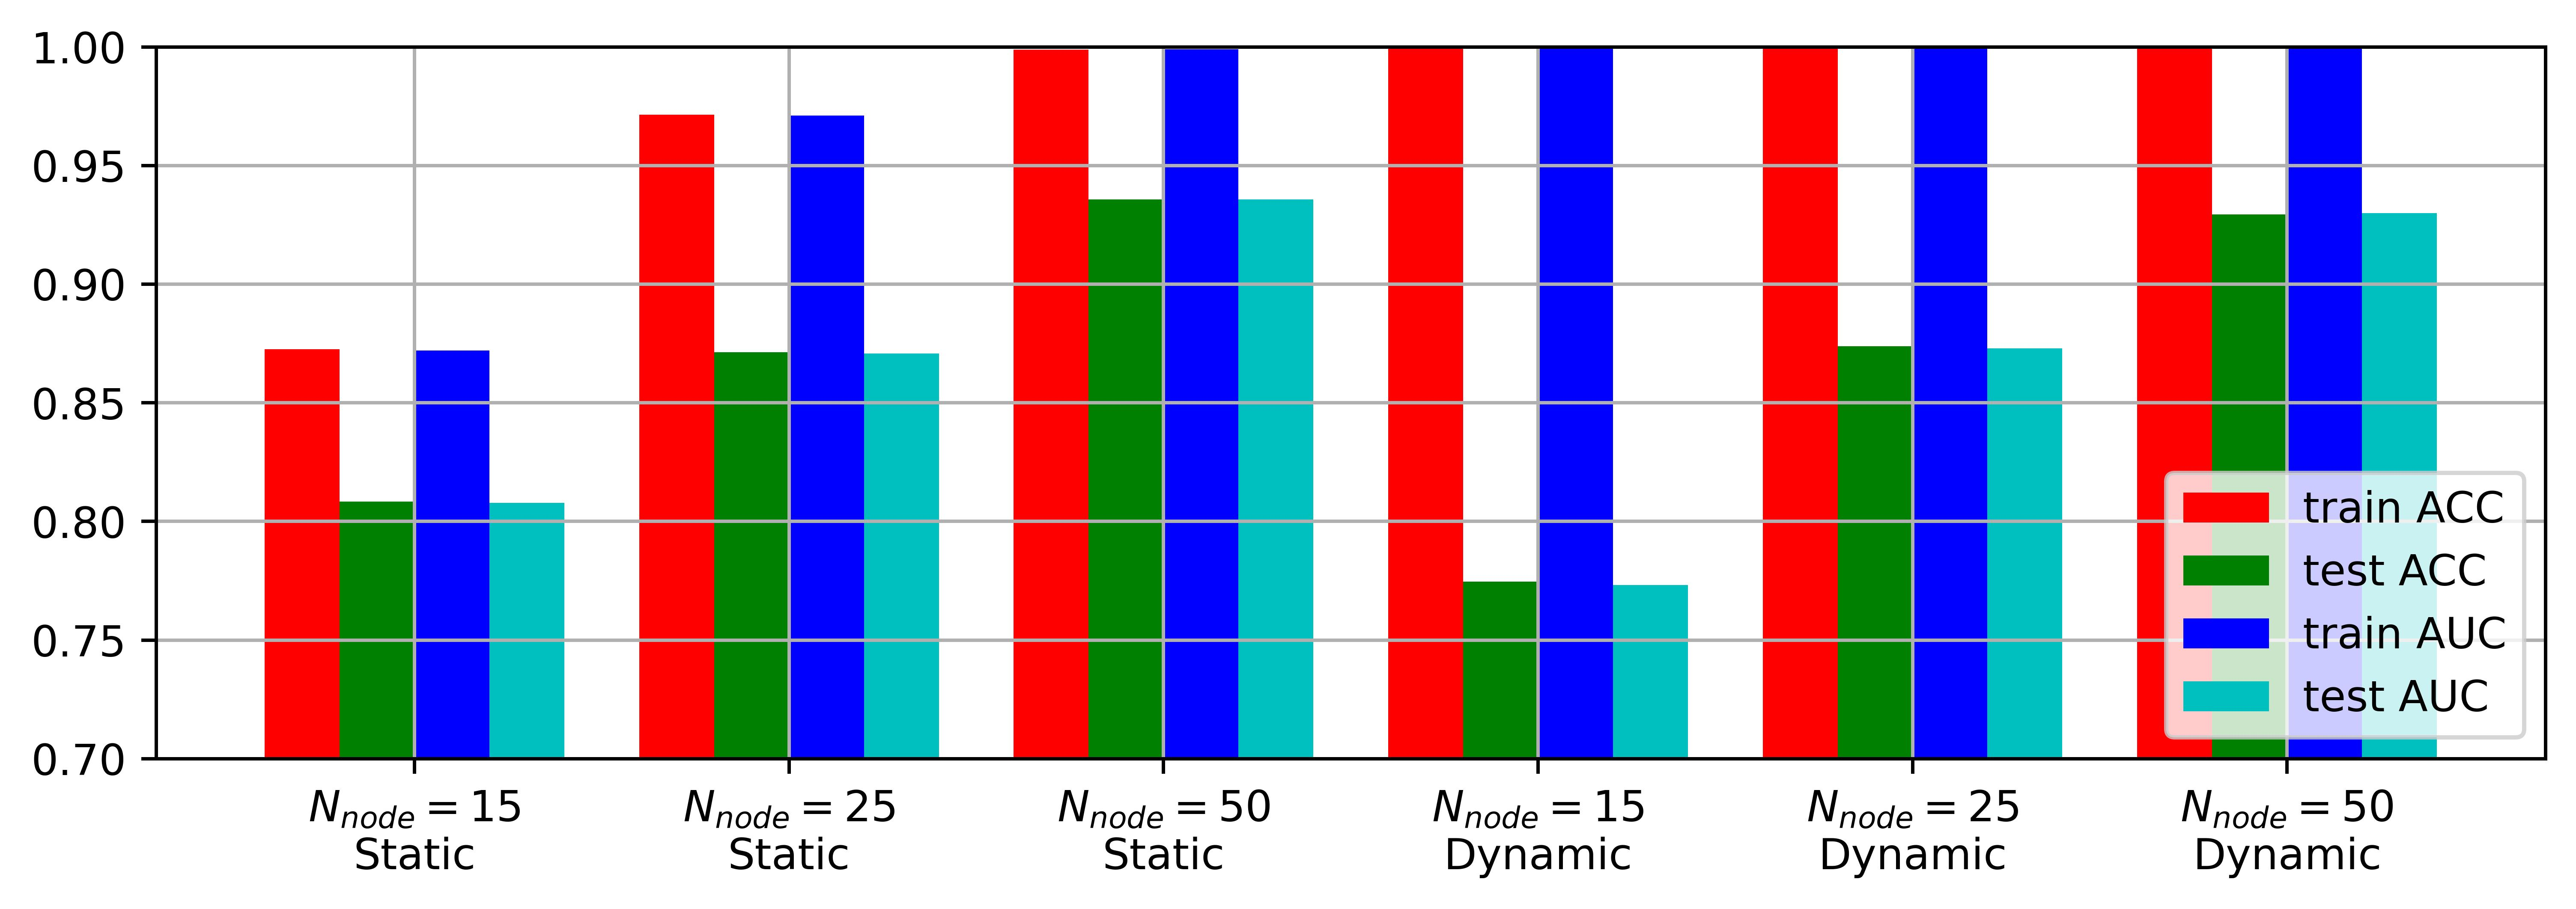
\includegraphics[width=0.6\textwidth]{../SVM/linear_0.1.jpg} \\
        \caption{Results of Linear SVM.}
    \end{figure}

    \begin{figure}[H]
        \centering
        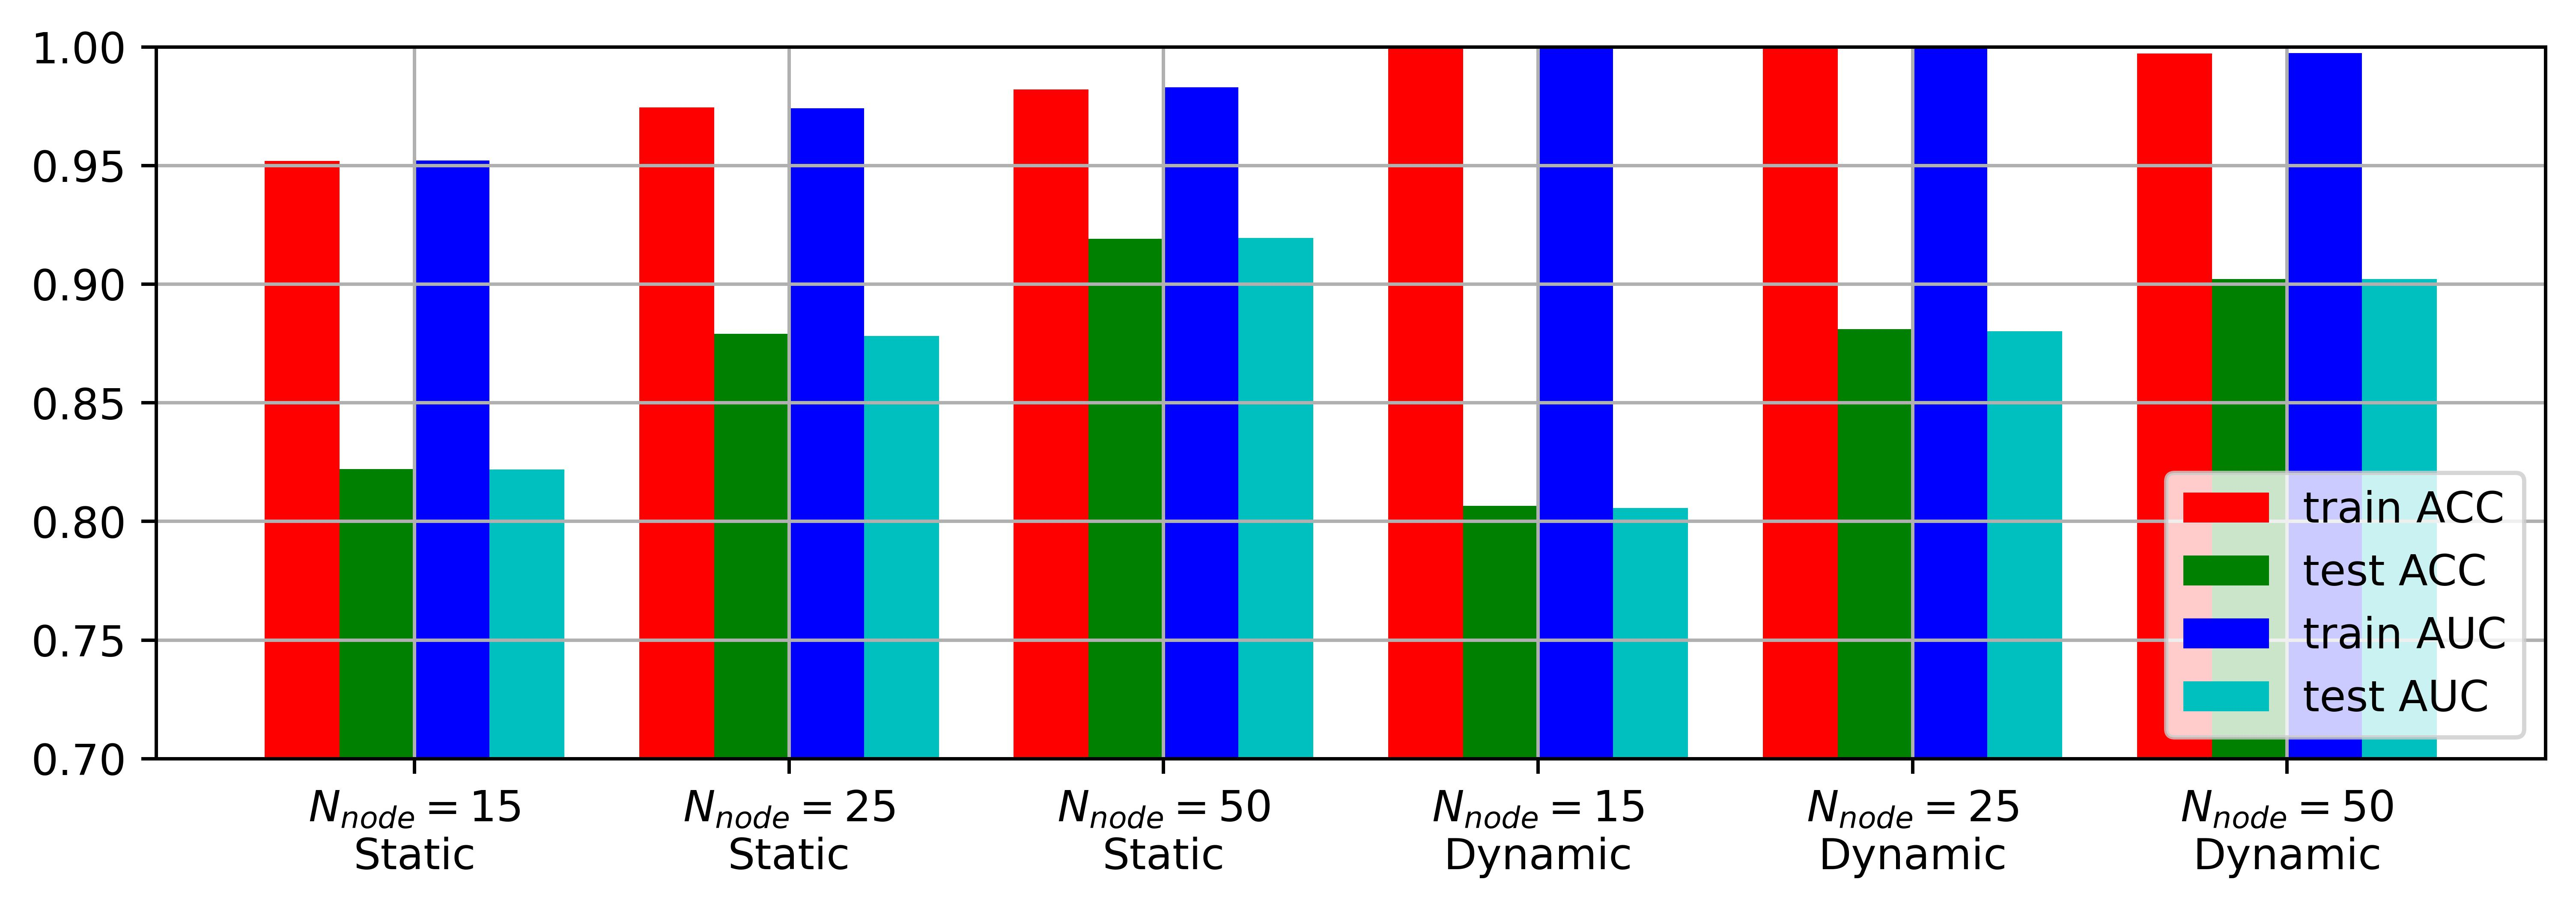
\includegraphics[width=0.6\textwidth]{../SVM/nu_0.1.jpg} \\
        \caption{Results of Nu-SVM.}
    \end{figure}

\end{frame}

\begin{frame}{CNN - Model}

    Given a dataset $\{ (\mathbf{x}_i, y_i) \}_{i=1}^N$, we aims to find some vectors $\{\mathbf{w}_k\}_{k=1}^m$ and some numbers $\{b_k\}_{k=1}^m$ such that any given data $\mathbf{x}$ can be classificated via the tuple of distance $( \mathbf{w}_1^T \mathbf{x} - b_1, \dots, \mathbf{w}_m^T \mathbf{x} - b_m )$.

    In the worst case, all the $\mathbf{w}_k$ and $b_k$ are the same, then the results should be the same with linear SVM.

    \begin{figure}[H]
        \centering
        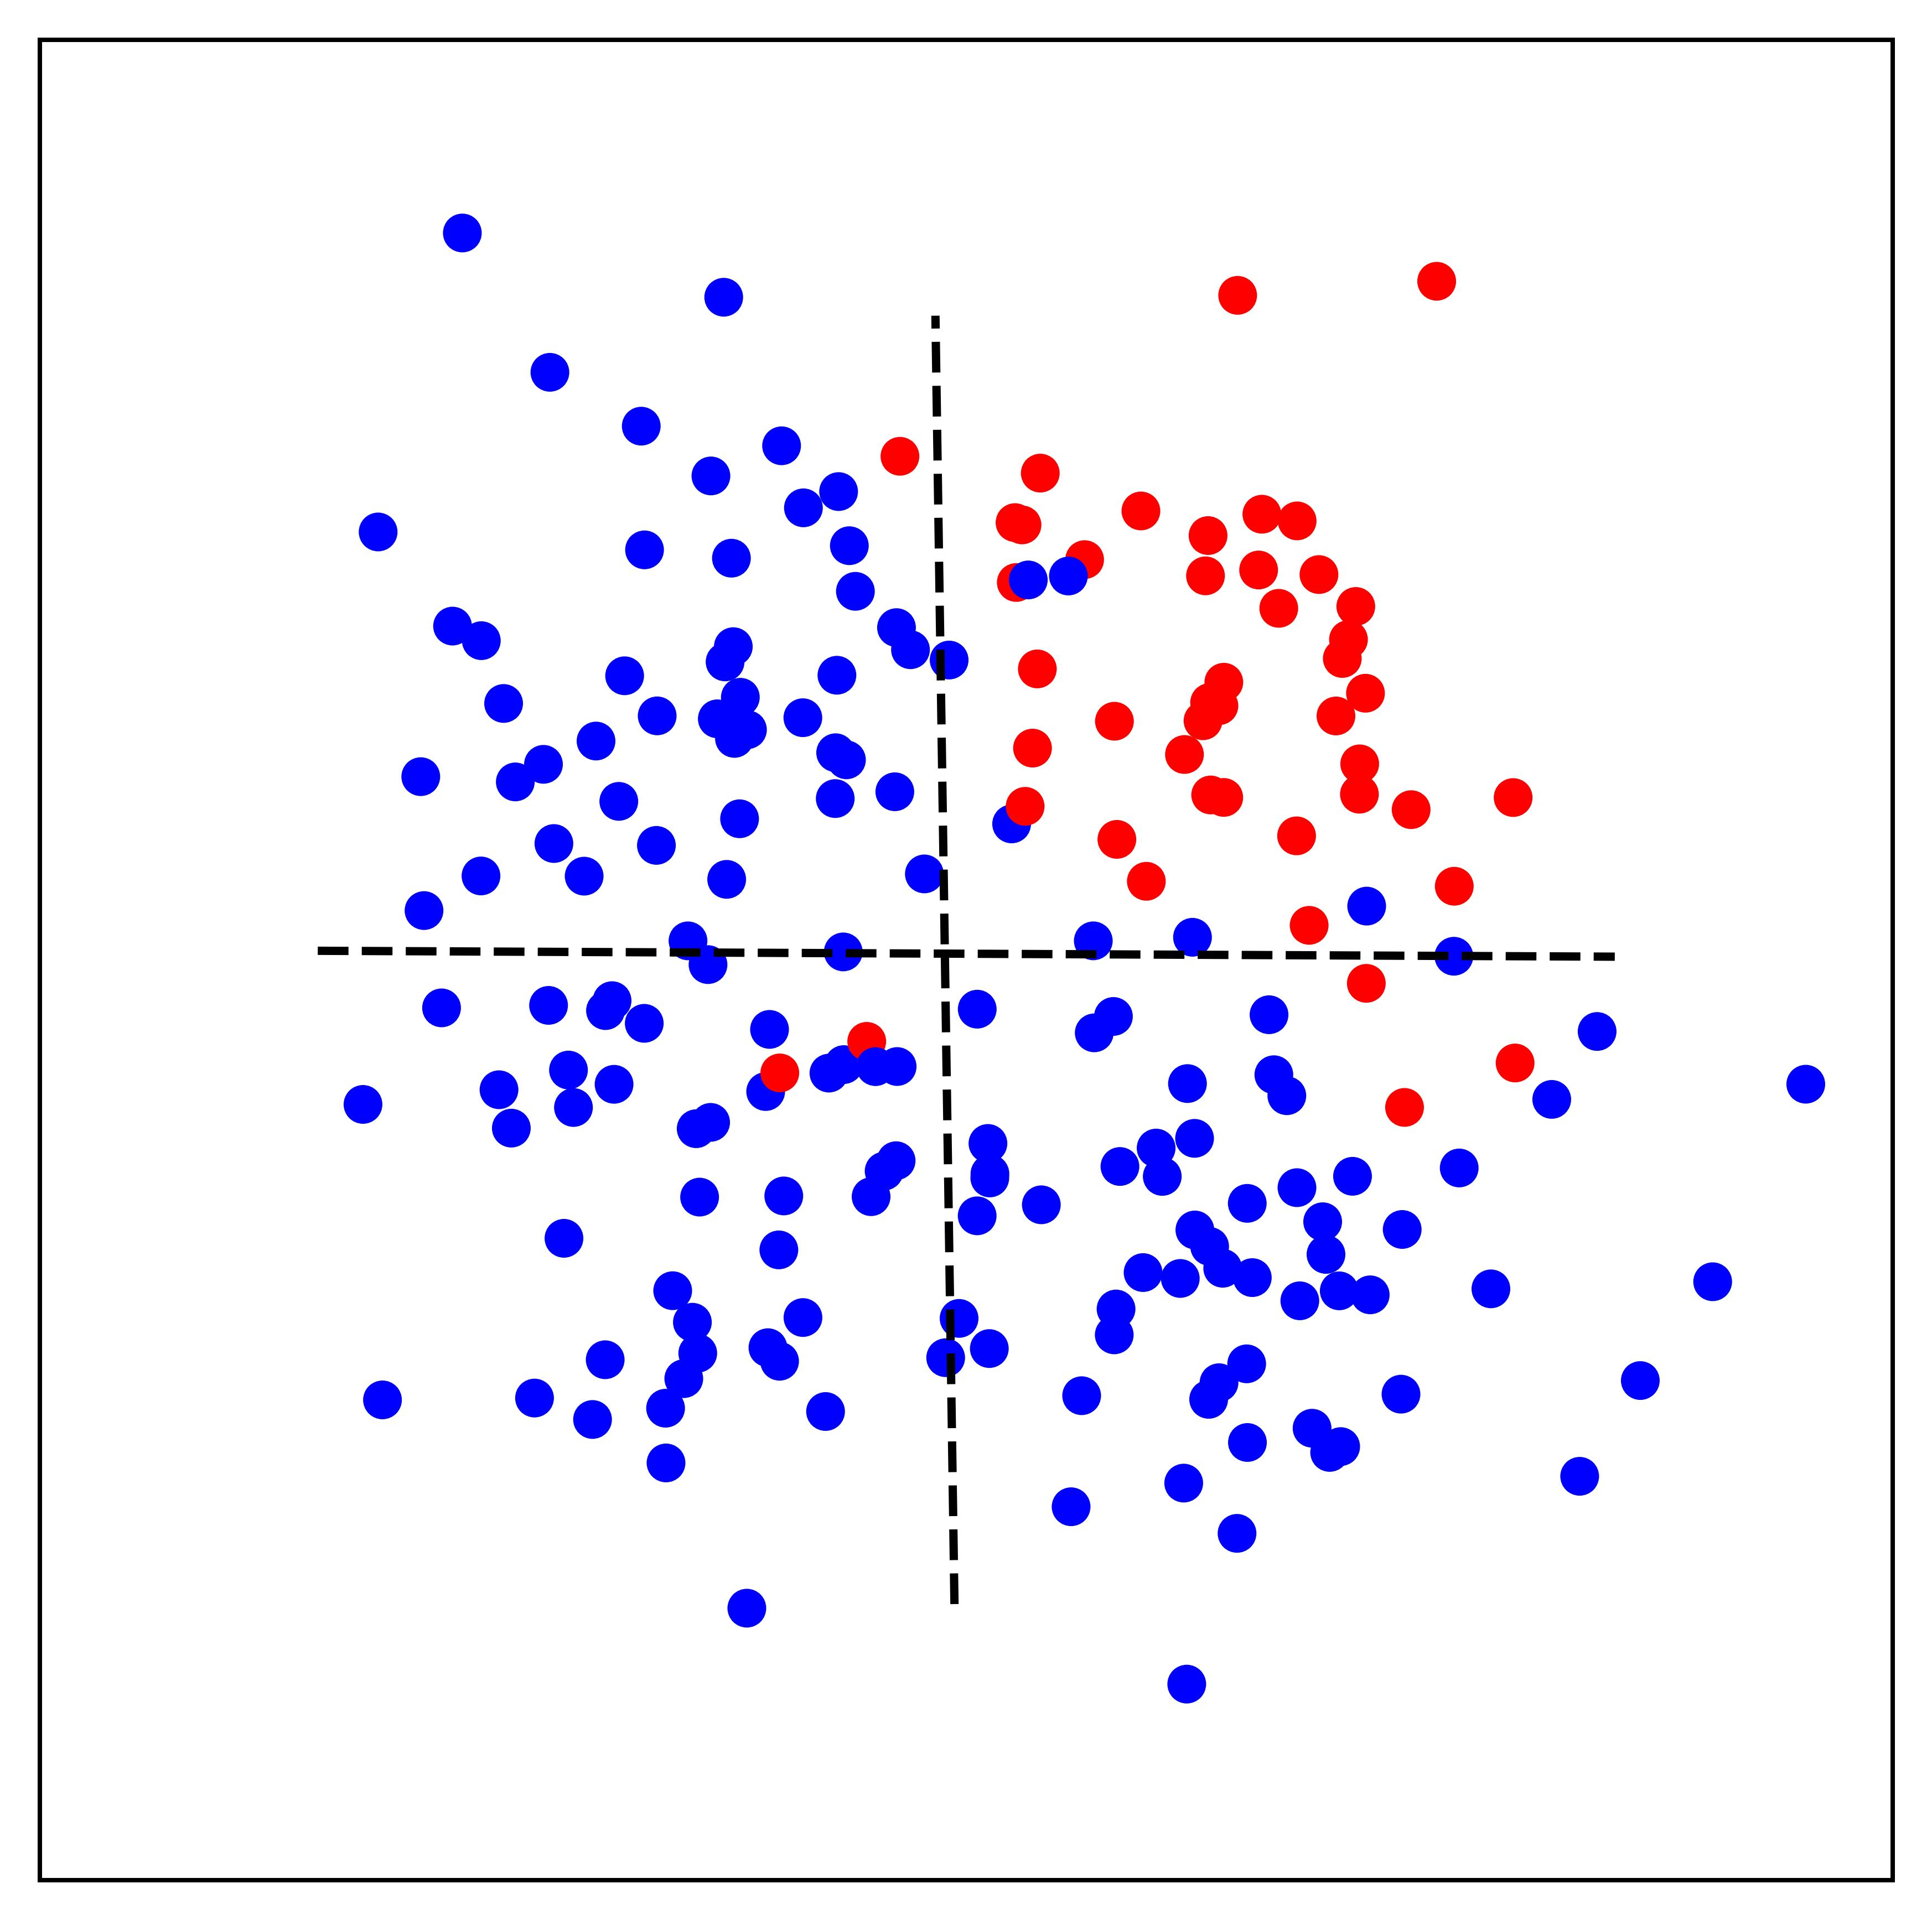
\includegraphics[width=0.3\textwidth]{./figure/model.jpg}
        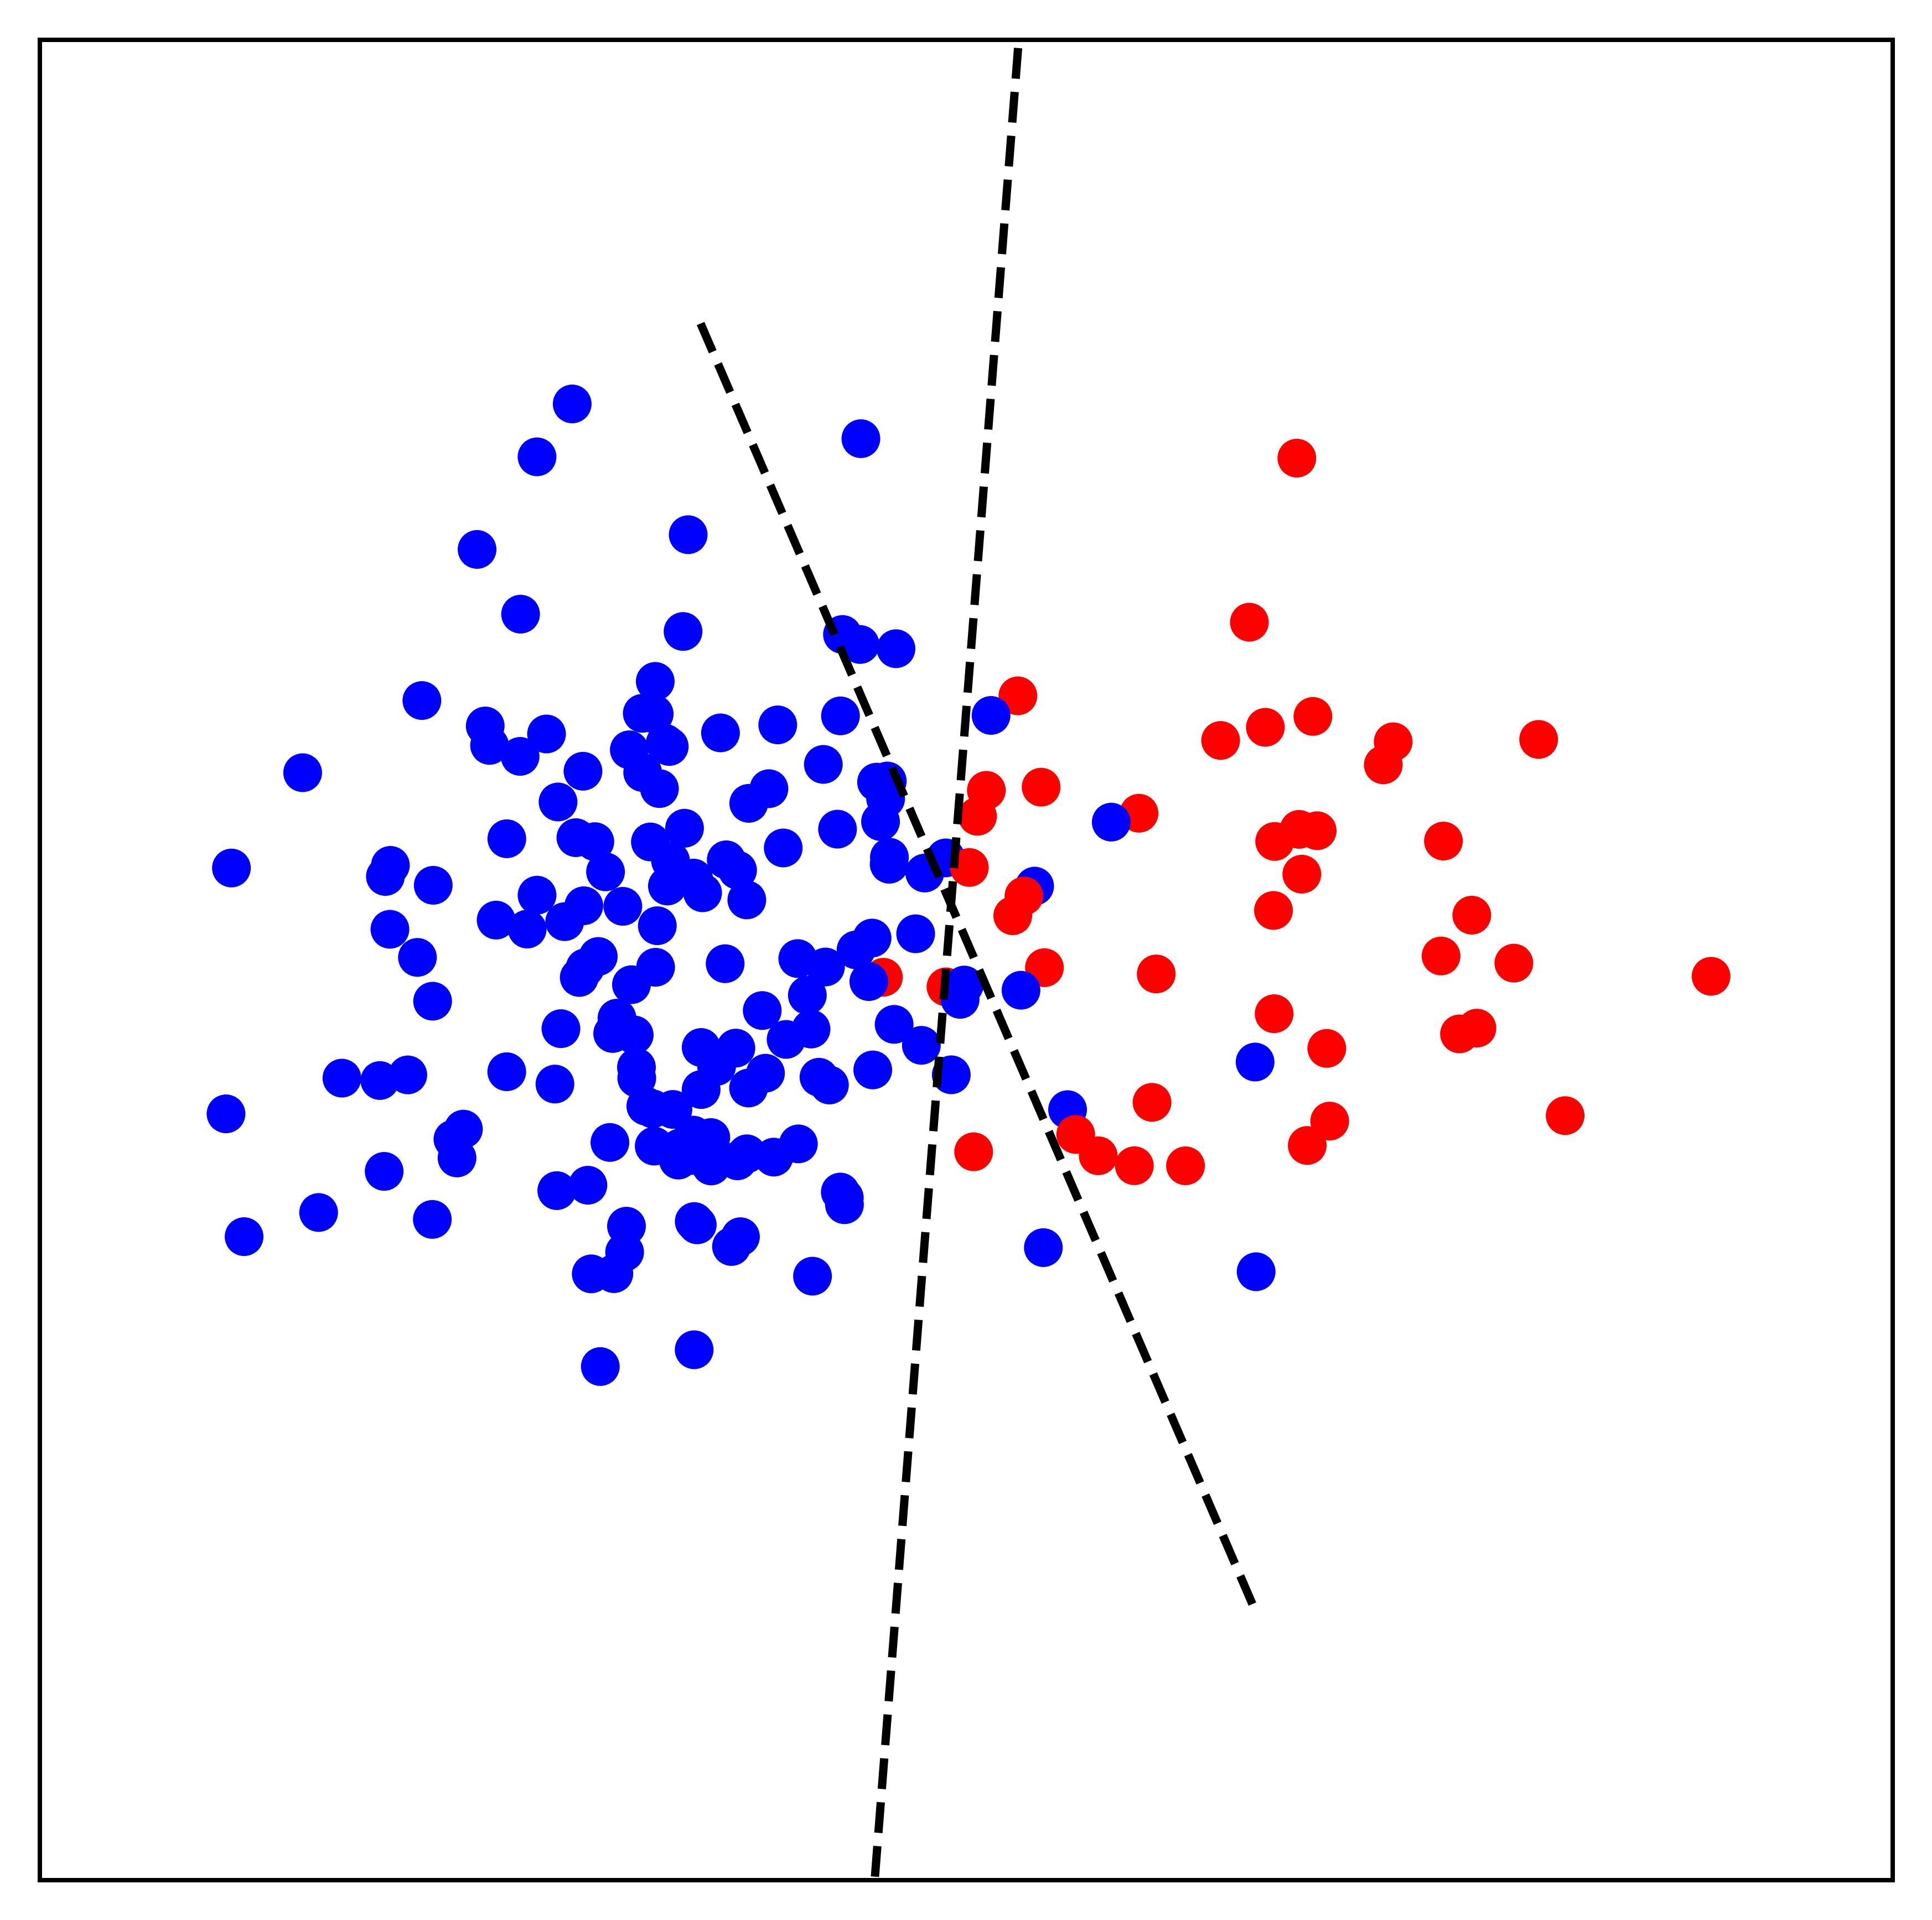
\includegraphics[width=0.3\textwidth]{./figure/model_worse.jpg}
    \end{figure}

\end{frame}

\begin{frame}{CNN - Model}

    The followings are the flowchart of our method, where we use a 1-layer 1-dimensional CNN with size equivalent to the input shape, so that it is the same as previous statements.

    \begin{figure}[H]
        \centering
        \includegraphics[width=0.8\textwidth]{./figure/method.png}
    \end{figure}

    We split the data into training dataset ($80\%$) and test dataset ($20\%$), and repeat the experiment for $150$ times to avoid flukes.

\end{frame}

\begin{frame}{CNN - Results}

    \begin{figure}[H]
        \centering
        \includegraphics[width=0.8\textwidth]{../Result/bar_channel=4_dropout=0.1.jpg} \\
        \subfloat[test ACC]{\includegraphics[width=0.4\textwidth]{../Result/test_acc_box_channel=4_dropout=0.1.jpg}}
        \subfloat[test AUC]{\includegraphics[width=0.4\textwidth]{../Result/test_auc_box_channel=4_dropout=0.1.jpg}}
        \caption{Results of CNN model with dropout = 0.1 and channel = 4.}
        % \label{CNN-results-3}
    \end{figure}

\end{frame}

\begin{frame}{CNN - Results}

    \begin{itemize}
        \item More nodes leads to a higher accuracy and AUC;
        \item The choise of sFC and dFC will not significantly affect the result;
        \item The accuracy rate will decrease when using the sub-series.
    \end{itemize}

\end{frame}

\section{Analysis}
\begin{frame}{LDA\footfullcite{Goldstein1976-aj}}

    Given a dataset $\{ \mathbf{x}_i, y_i \}_{i=1}^N$, the LDA aims to find a vector pair $\mathbf{y}, \mathbf{c}$ such that the inner product $\langle \mathbf{x}_i - \mathbf{c}, \mathbf{y} \rangle$ minimizes the interclass variance and maximizes the distance between the projected means of the classes.

    \begin{figure}[H]
        \centering
        \includegraphics[width=0.6\textwidth]{./figure/lda.jpg}
    \end{figure}

\end{frame}

\begin{frame}{LDA - sFC}

    \begin{figure}[H]
        \centering
        \subfloat[$N_{node} = 15$]{
            \begin{minipage}[b]{0.3\textwidth}
                \includegraphics[width=1\textwidth]{../Analysis/LDA/node=15_size=4800_step=4800_rho=0.1/hist_0.jpg}
                \includegraphics[width=1\textwidth]{../Analysis/LDA/node=15_size=4800_step=4800_rho=0.1/box_0.jpg}
            \end{minipage}
        }
        \subfloat[$N_{node} = 25$]{
            \begin{minipage}[b]{0.3\textwidth}
                \includegraphics[width=1\textwidth]{../Analysis/LDA/node=25_size=4800_step=4800_rho=0.1/hist_0.jpg}
                \includegraphics[width=1\textwidth]{../Analysis/LDA/node=25_size=4800_step=4800_rho=0.1/box_0.jpg}
            \end{minipage}
        }
        \subfloat[$N_{node} = 50$]{
            \begin{minipage}[b]{0.3\textwidth}
                \includegraphics[width=1\textwidth]{../Analysis/LDA/node=50_size=4800_step=4800_rho=0.1/hist_0.jpg}
                \includegraphics[width=1\textwidth]{../Analysis/LDA/node=50_size=4800_step=4800_rho=0.1/box_0.jpg}
            \end{minipage}
        }
        \caption{LDA for sFC.}
        % \label{LDA-example-1}
    \end{figure}

\end{frame}

% \begin{frame}{LDA - sFC}

%     \begin{figure}[H]
%         \centering
%         \subfloat[$N_{node} = 15$]{
%             \begin{minipage}[b]{0.3\textwidth}
%                 \includegraphics[width=1\textwidth]{../Analysis/LDA_split/node=15_size=4800_step=4800_rho=0.1/hist_test.jpg}
%                 \includegraphics[width=1\textwidth]{../Analysis/LDA_split/node=15_size=4800_step=4800_rho=0.1/box_test.jpg}
%             \end{minipage}
%         }
%         \subfloat[$N_{node} = 25$]{
%             \begin{minipage}[b]{0.3\textwidth}
%                 \includegraphics[width=1\textwidth]{../Analysis/LDA_split/node=25_size=4800_step=4800_rho=0.1/hist_test.jpg}
%                 \includegraphics[width=1\textwidth]{../Analysis/LDA_split/node=25_size=4800_step=4800_rho=0.1/box_test.jpg}
%             \end{minipage}
%         }
%         \subfloat[$N_{node} = 50$]{
%             \begin{minipage}[b]{0.3\textwidth}
%                 \includegraphics[width=1\textwidth]{../Analysis/LDA_split/node=50_size=4800_step=4800_rho=0.1/hist_test.jpg}
%                 \includegraphics[width=1\textwidth]{../Analysis/LDA_split/node=50_size=4800_step=4800_rho=0.1/box_test.jpg}
%             \end{minipage}
%         }
%         \caption{The LDA model fits the train set ($80\%$) and applies on test set ($20\%$).}
%         % \label{LDA-example-1}
%     \end{figure}

% \end{frame}

\begin{frame}{LDA - dFC}

    \begin{figure}[H]
        \centering
        \subfloat[$N_{node} = 15$]{
            \begin{minipage}[b]{0.3\textwidth}
                \includegraphics[width=1\textwidth]{../Analysis/LDA/node=15_size=480_step=180_rho=0.1/hist.jpg}
                \includegraphics[width=1\textwidth]{../Analysis/LDA/node=15_size=480_step=180_rho=0.1/box.jpg}
            \end{minipage}
        }
        \subfloat[$N_{node} = 25$]{
            \begin{minipage}[b]{0.3\textwidth}
                \includegraphics[width=1\textwidth]{../Analysis/LDA/node=25_size=480_step=180_rho=0.1/hist.jpg}
                \includegraphics[width=1\textwidth]{../Analysis/LDA/node=25_size=480_step=180_rho=0.1/box.jpg}
            \end{minipage}
        }
        \subfloat[$N_{node} = 50$]{
            \begin{minipage}[b]{0.3\textwidth}
                \includegraphics[width=1\textwidth]{../Analysis/LDA/node=50_size=480_step=180_rho=0.1/hist.jpg}
                \includegraphics[width=1\textwidth]{../Analysis/LDA/node=50_size=480_step=180_rho=0.1/box.jpg}
            \end{minipage}
        }
        \caption{LDA for dFC.}
        % \label{LDA-example-1}
    \end{figure}

\end{frame}

\begin{frame}{LDA - dFC}

    \begin{figure}[H]
        \centering
        \subfloat[$N_{node} = 15$]{
            \begin{minipage}[b]{0.3\textwidth}
                \includegraphics[width=1\textwidth]{../Analysis/LDA/node=15_size=480_step=180_rho=0.1/hist_11.jpg}
                \includegraphics[width=1\textwidth]{../Analysis/LDA/node=15_size=480_step=180_rho=0.1/box_11.jpg}
            \end{minipage}
        }
        \subfloat[$N_{node} = 25$]{
            \begin{minipage}[b]{0.3\textwidth}
                \includegraphics[width=1\textwidth]{../Analysis/LDA/node=25_size=480_step=180_rho=0.1/hist_6.jpg}
                \includegraphics[width=1\textwidth]{../Analysis/LDA/node=25_size=480_step=180_rho=0.1/box_6.jpg}
            \end{minipage}
        }
        \subfloat[$N_{node} = 50$]{
            \begin{minipage}[b]{0.3\textwidth}
                \includegraphics[width=1\textwidth]{../Analysis/LDA/node=50_size=480_step=180_rho=0.1/hist_11.jpg}
                \includegraphics[width=1\textwidth]{../Analysis/LDA/node=50_size=480_step=180_rho=0.1/box_11.jpg}
            \end{minipage}
        }
        \caption{LDA for 1-frame of dFC with max score.}
        % \label{LDA-example-1}
    \end{figure}

\end{frame}

\begin{frame}{LDA - dFC}

    \begin{figure}[H]
        \centering
        \subfloat[$N_{node} = 15$]{
            \begin{minipage}[b]{0.3\textwidth}
                \includegraphics[width=1\textwidth]{../Analysis/LDA/node=15_size=480_step=180_rho=0.1/hist_10.jpg}
                \includegraphics[width=1\textwidth]{../Analysis/LDA/node=15_size=480_step=180_rho=0.1/box_10.jpg}
            \end{minipage}
        }
        \subfloat[$N_{node} = 25$]{
            \begin{minipage}[b]{0.3\textwidth}
                \includegraphics[width=1\textwidth]{../Analysis/LDA/node=25_size=480_step=180_rho=0.1/hist_13.jpg}
                \includegraphics[width=1\textwidth]{../Analysis/LDA/node=25_size=480_step=180_rho=0.1/box_13.jpg}
            \end{minipage}
        }
        \subfloat[$N_{node} = 50$]{
            \begin{minipage}[b]{0.3\textwidth}
                \includegraphics[width=1\textwidth]{../Analysis/LDA/node=50_size=480_step=180_rho=0.1/hist_16.jpg}
                \includegraphics[width=1\textwidth]{../Analysis/LDA/node=50_size=480_step=180_rho=0.1/box_16.jpg}
            \end{minipage}
        }
        \caption{LDA for 1-frame of dFC with min score.}
        % \label{LDA-example-1}
    \end{figure}

\end{frame}

% \begin{frame}{LDA - dFC}

%     \begin{figure}[H]
%         \centering
%         \subfloat[$N_{node} = 15$]{
%             \begin{minipage}[b]{0.3\textwidth}
%                 \includegraphics[width=1\textwidth]{../Analysis/LDA_split/node=15_size=480_step=180_rho=0.1/hist_test.jpg}
%                 \includegraphics[width=1\textwidth]{../Analysis/LDA_split/node=15_size=480_step=180_rho=0.1/box_test.jpg}
%             \end{minipage}
%         }
%         \subfloat[$N_{node} = 25$]{
%             \begin{minipage}[b]{0.3\textwidth}
%                 \includegraphics[width=1\textwidth]{../Analysis/LDA_split/node=25_size=480_step=180_rho=0.1/hist_test.jpg}
%                 \includegraphics[width=1\textwidth]{../Analysis/LDA_split/node=25_size=480_step=180_rho=0.1/box_test.jpg}
%             \end{minipage}
%         }
%         \subfloat[$N_{node} = 50$]{
%             \begin{minipage}[b]{0.3\textwidth}
%                 \includegraphics[width=1\textwidth]{../Analysis/LDA_split/node=50_size=480_step=180_rho=0.1/hist_test.jpg}
%                 \includegraphics[width=1\textwidth]{../Analysis/LDA_split/node=50_size=480_step=180_rho=0.1/box_test.jpg}
%             \end{minipage}
%         }
%         \caption{The LDA model fits the train set ($80\%$) and applies on test set ($20\%$).}
%         % \label{LDA-example-1}
%     \end{figure}

% \end{frame}

% \begin{frame}{LDA - dFC}

%     \begin{figure}[H]
%         \centering
%         \subfloat[]{
%             \begin{minipage}[b]{0.3\textwidth}
%                 \includegraphics[width=1\textwidth]{../Analysis/LDA/node=15_size=480_step=180_rho=0.1/hist_0.jpg}
%                 \includegraphics[width=1\textwidth]{../Analysis/LDA/node=15_size=480_step=180_rho=0.1/box_0.jpg}
%             \end{minipage}
%         }
%         \subfloat[]{
%             \begin{minipage}[b]{0.3\textwidth}
%                 \includegraphics[width=1\textwidth]{../Analysis/LDA/node=15_size=480_step=180_rho=0.1/hist_10.jpg}
%                 \includegraphics[width=1\textwidth]{../Analysis/LDA/node=15_size=480_step=180_rho=0.1/box_10.jpg}
%             \end{minipage}
%         }
%         \subfloat[]{
%             \begin{minipage}[b]{0.3\textwidth}
%                 \includegraphics[width=1\textwidth]{../Analysis/LDA/node=15_size=480_step=180_rho=0.1/hist_20.jpg}
%                 \includegraphics[width=1\textwidth]{../Analysis/LDA/node=15_size=480_step=180_rho=0.1/box_20.jpg}
%             \end{minipage}
%         }
%         \caption{LDA for dFC with $N_{node} = 15$.}
%         % \label{LDA-example-1}
%     \end{figure}

% \end{frame}

% \begin{frame}{LDA - dFC}

%     \begin{figure}[H]
%         \centering
%         \subfloat[]{
%             \begin{minipage}[b]{0.3\textwidth}
%                 \includegraphics[width=1\textwidth]{../Analysis/LDA/node=25_size=480_step=180_rho=0.1/hist_0.jpg}
%                 \includegraphics[width=1\textwidth]{../Analysis/LDA/node=25_size=480_step=180_rho=0.1/box_0.jpg}
%             \end{minipage}
%         }
%         \subfloat[]{
%             \begin{minipage}[b]{0.3\textwidth}
%                 \includegraphics[width=1\textwidth]{../Analysis/LDA/node=25_size=480_step=180_rho=0.1/hist_10.jpg}
%                 \includegraphics[width=1\textwidth]{../Analysis/LDA/node=25_size=480_step=180_rho=0.1/box_10.jpg}
%             \end{minipage}
%         }
%         \subfloat[]{
%             \begin{minipage}[b]{0.3\textwidth}
%                 \includegraphics[width=1\textwidth]{../Analysis/LDA/node=25_size=480_step=180_rho=0.1/hist_20.jpg}
%                 \includegraphics[width=1\textwidth]{../Analysis/LDA/node=25_size=480_step=180_rho=0.1/box_20.jpg}
%             \end{minipage}
%         }
%         \caption{LDA for dFC with $N_{node} = 25$.}
%         % \label{LDA-example-1}
%     \end{figure}

% \end{frame}

% \begin{frame}{LDA - dFC}

%     \begin{figure}[H]
%         \centering
%         \subfloat[]{
%             \begin{minipage}[b]{0.3\textwidth}
%                 \includegraphics[width=1\textwidth]{../Analysis/LDA/node=50_size=480_step=180_rho=0.1/hist_0.jpg}
%                 \includegraphics[width=1\textwidth]{../Analysis/LDA/node=50_size=480_step=180_rho=0.1/box_0.jpg}
%             \end{minipage}
%         }
%         \subfloat[]{
%             \begin{minipage}[b]{0.3\textwidth}
%                 \includegraphics[width=1\textwidth]{../Analysis/LDA/node=50_size=480_step=180_rho=0.1/hist_10.jpg}
%                 \includegraphics[width=1\textwidth]{../Analysis/LDA/node=50_size=480_step=180_rho=0.1/box_10.jpg}
%             \end{minipage}
%         }
%         \subfloat[]{
%             \begin{minipage}[b]{0.3\textwidth}
%                 \includegraphics[width=1\textwidth]{../Analysis/LDA/node=50_size=480_step=180_rho=0.1/hist_20.jpg}
%                 \includegraphics[width=1\textwidth]{../Analysis/LDA/node=50_size=480_step=180_rho=0.1/box_20.jpg}
%             \end{minipage}
%         }
%         \caption{LDA for dFC with $N_{node} = 50$.}
%         % \label{LDA-example-1}
%     \end{figure}

% \end{frame}

\begin{frame}{LDA - Results}

    \begin{itemize}
        \item Both sFC and dFC is linear separable;
        \item The overlap become less with the increase of node;
        \item The dFC is not always better than sFC, especially when there exists some outliers.
    \end{itemize}

\end{frame}

\section{Discussion}
\begin{frame}{Discussion}

    \begin{itemize}
        \item Both sFC and dFC is linear separable;
        \item Both sFC and dFC can be used to predict gender with high accuracy and AUC;
        \item More nodes leads to a higher accuracy and AUC;
        \item The choise of sFC and dFC will not significantly affect the accuracy rate and AUC;
        \item The brain noise\footnote{spontaneous fluctuations in the electrical activity of the neurons} will affect more on the dFC.
    \end{itemize}

\end{frame}

\begin{frame}{Future research directions}

    \begin{itemize}
        \item Choose a more reasonable size and step of the window via Fourier analysis, wavelet analysis, etc;
        \item Force the coefficient of CNN to be orthogonal;
        \item Use some simple nonlinear classifier (i.e. quadratic classifier);
        \item Use effective connectivity as input.
    \end{itemize}

\end{frame}

\section*{Reference}
\begin{frame}[allowframebreaks]{Reference}
    \printbibliography
\end{frame}

\appendix

\section{Ablation study}

\begin{frame}{Ablation study - SVM}
    \begin{table}[H]
        \centering
        \begin{tabular}{|c|c|c|c|c|}
            \hline
            Node & Data & min ACC/AUC       & mean ACC/AUC      & max ACC/AUC       \\
            \hline
            $15$ & sFC  & $0.7363$/$0.7369$ & $0.8083$/$0.8078$ & $0.8706$/$0.8756$ \\
            \hline
            $25$ & sFC  & $0.8060$/$0.8059$ & $0.8714$/$0.8708$ & $0.9204$/$0.9202$ \\
            \hline
            $50$ & sFC  & $0.8905$/$0.8905$ & $0.9357$/$0.9357$ & $0.9751$/$0.9749$ \\
            \hline
            $15$ & dFC  & $0.6866$/$0.6919$ & $0.7746$/$0.7733$ & $0.8507$/$0.8534$ \\
            \hline
            $25$ & dFC  & $0.7861$/$0.7874$ & $0.8739$/$0.8730$ & $0.9204$/$0.9206$ \\
            \hline
            $50$ & dFC  & $0.8806$/$0.8813$ & $0.9295$/$0.9300$ & $0.9652$/$0.9666$ \\
            \hline
        \end{tabular}
        \caption{Ablation study for LinearSVM.}
    \end{table}
\end{frame}

\begin{frame}{Ablation study - SVM}
    \begin{table}[H]
        \centering
        \begin{tabular}{|c|c|c|c|c|}
            \hline
            Node & Data & min ACC/AUC       & mean ACC/AUC      & max ACC/AUC       \\
            \hline
            $15$ & sFC  & $0.7562$/$0.7571$ & $0.8221$/$0.8219$ & $0.8856$/$0.8847$ \\
            \hline
            $25$ & sFC  & $0.8259$/$0.8257$ & $0.8791$/$0.8782$ & $0.9303$/$0.9302$ \\
            \hline
            $50$ & sFC  & $0.8458$/$0.8458$ & $0.9191$/$0.9194$ & $0.9602$/$0.9608$ \\
            \hline
            $15$ & dFC  & $0.7313$/$0.7324$ & $0.8066$/$0.8056$ & $0.8706$/$0.8674$ \\
            \hline
            $25$ & dFC  & $0.8109$/$0.8121$ & $0.8811$/$0.8802$ & $0.9303$/$0.9296$ \\
            \hline
            $50$ & dFC  & $0.8308$/$0.8300$ & $0.9021$/$0.9022$ & $0.9552$/$0.9579$ \\
            \hline
        \end{tabular}
        \caption{Ablation study for NuSVM.}
    \end{table}
\end{frame}

\begin{frame}{Ablation study - SVM}

    \begin{figure}[H]
        \subfloat[test ACC for LinearSVM]{\includegraphics[width=0.4\textwidth]{../SVM/acc_linear_0.1.jpg}}
        \subfloat[test AUC for LinearSVM]{\includegraphics[width=0.4\textwidth]{../SVM/auc_linear_0.1.jpg}} \\
        \subfloat[test ACC for NuSVM]{\includegraphics[width=0.4\textwidth]{../SVM/acc_nu_0.1.jpg}}
        \subfloat[test AUC for NuSVM]{\includegraphics[width=0.4\textwidth]{../SVM/auc_nu_0.1.jpg}} \\
        \caption{Results of SVM.}
        % \label{CNN-results-3}
    \end{figure}

\end{frame}

\begin{frame}{Ablation study - CNN}

    \begin{table}[H]
        \centering
        \begin{tabular}{|c|c|c|c|c|c|}
            \hline
            Data & DR    & CH  & min ACC/AUC       & mean ACC/AUC      & max ACC/AUC       \\
            \hline
            sFC  & $0.0$ & $1$ & $0.5224$/$0.8108$ & $0.7957$/$0.8855$ & $0.8706$/$0.9307$ \\
            \hline
            sFC  & $0.0$ & $2$ & $0.7164$/$0.8273$ & $0.8001$/$0.8876$ & $0.8756$/$0.9281$ \\
            \hline
            sFC  & $0.0$ & $4$ & $0.7363$/$0.8189$ & $0.7988$/$0.8863$ & $0.8607$/$0.9337$ \\
            \hline
            sFC  & $0.1$ & $1$ & $0.5174$/$0.8041$ & $0.7952$/$0.8870$ & $0.8756$/$0.9355$ \\
            \hline
            sFC  & $0.1$ & $2$ & $0.7164$/$0.8318$ & $0.7986$/$0.8885$ & $0.8756$/$0.9294$ \\
            \hline
            sFC  & $0.1$ & $4$ & $0.7313$/$0.8276$ & $0.8038$/$0.8911$ & $0.8607$/$0.9317$ \\
            \hline
            dFC  & $0.0$ & $1$ & $0.5871$/$0.7160$ & $0.7737$/$0.8670$ & $0.8557$/$0.9216$ \\
            \hline
            dFC  & $0.0$ & $2$ & $0.6915$/$0.7824$ & $0.7811$/$0.8630$ & $0.8507$/$0.9209$ \\
            \hline
            dFC  & $0.0$ & $4$ & $0.7015$/$0.8028$ & $0.7787$/$0.8584$ & $0.8408$/$0.9148$ \\
            \hline
            dFC  & $0.1$ & $1$ & $0.5522$/$0.7140$ & $0.7735$/$0.8656$ & $0.8458$/$0.9209$ \\
            \hline
            dFC  & $0.1$ & $2$ & $0.6617$/$0.7942$ & $0.7771$/$0.8692$ & $0.8408$/$0.9110$ \\
            \hline
            dFC  & $0.1$ & $4$ & $0.7164$/$0.7987$ & $0.7813$/$0.8666$ & $0.8408$/$0.9171$ \\
            \hline
        \end{tabular}
        \caption{Ablation study for $N_{node} = 15$.}
    \end{table}

\end{frame}

\begin{frame}{Ablation study - CNN}

    \begin{table}[H]
        \centering
        \begin{tabular}{|c|c|c|c|c|c|}
            \hline
            Data & DR    & CH  & min ACC/AUC       & mean ACC/AUC      & max ACC/AUC       \\
            \hline
            sFC  & $0.0$ & $1$ & $0.5075$/$0.7475$ & $0.8462$/$0.9265$ & $0.9104$/$0.9634$ \\
            \hline
            sFC  & $0.0$ & $2$ & $0.7662$/$0.8731$ & $0.8470$/$0.9225$ & $0.9104$/$0.9599$ \\
            \hline
            sFC  & $0.0$ & $4$ & $0.7512$/$0.8650$ & $0.8468$/$0.9220$ & $0.9055$/$0.9603$ \\
            \hline
            sFC  & $0.1$ & $1$ & $0.5124$/$0.7431$ & $0.8547$/$0.9356$ & $0.9154$/$0.9688$ \\
            \hline
            sFC  & $0.1$ & $2$ & $0.7711$/$0.8598$ & $0.8581$/$0.9358$ & $0.9254$/$0.9728$ \\
            \hline
            sFC  & $0.1$ & $4$ & $0.7711$/$0.8730$ & $0.8562$/$0.9339$ & $0.9104$/$0.9638$ \\
            \hline
            dFC  & $0.0$ & $1$ & $0.6269$/$0.7168$ & $0.8450$/$0.9338$ & $0.9303$/$0.9788$ \\
            \hline
            dFC  & $0.0$ & $2$ & $0.7463$/$0.8662$ & $0.8594$/$0.9416$ & $0.9254$/$0.9787$ \\
            \hline
            dFC  & $0.0$ & $4$ & $0.7960$/$0.9130$ & $0.8672$/$0.9437$ & $0.9154$/$0.9783$ \\
            \hline
            dFC  & $0.1$ & $1$ & $0.5771$/$0.6996$ & $0.8391$/$0.9319$ & $0.9254$/$0.9753$ \\
            \hline
            dFC  & $0.1$ & $2$ & $0.7612$/$0.8584$ & $0.8618$/$0.9441$ & $0.9204$/$0.9752$ \\
            \hline
            dFC  & $0.1$ & $4$ & $0.7264$/$0.8902$ & $0.8606$/$0.9426$ & $0.9104$/$0.9739$ \\
            \hline
        \end{tabular}
        \caption{Ablation study for $N_{node} = 25$.}
    \end{table}

\end{frame}

\begin{frame}{Ablation study - CNN}

    \begin{table}[H]
        \centering
        \begin{tabular}{|c|c|c|c|c|c|}
            \hline
            Data & DR    & CH  & min ACC/AUC       & mean ACC/AUC      & max ACC/AUC       \\
            \hline
            sFC  & $0.0$ & $1$ & $0.5572$/$0.7721$ & $0.9015$/$0.9689$ & $0.9602$/$0.9947$ \\
            \hline
            sFC  & $0.0$ & $2$ & $0.7512$/$0.8462$ & $0.9218$/$0.9762$ & $0.9701$/$0.9941$ \\
            \hline
            sFC  & $0.0$ & $4$ & $0.8856$/$0.9589$ & $0.9248$/$0.9779$ & $0.9602$/$0.9938$ \\
            \hline
            sFC  & $0.1$ & $1$ & $0.5124$/$0.7691$ & $0.8960$/$0.9684$ & $0.9652$/$0.9952$ \\
            \hline
            sFC  & $0.1$ & $2$ & $0.7363$/$0.8335$ & $0.9147$/$0.9746$ & $0.9652$/$0.9947$ \\
            \hline
            sFC  & $0.1$ & $4$ & $0.8358$/$0.9562$ & $0.9178$/$0.9778$ & $0.9652$/$0.9940$ \\
            \hline
            dFC  & $0.0$ & $1$ & $0.6766$/$0.8767$ & $0.8799$/$0.9689$ & $0.9552$/$0.9924$ \\
            \hline
            dFC  & $0.0$ & $2$ & $0.7711$/$0.9366$ & $0.9041$/$0.9733$ & $0.9552$/$0.9917$ \\
            \hline
            dFC  & $0.0$ & $4$ & $0.8507$/$0.9543$ & $0.9122$/$0.9766$ & $0.9602$/$0.9946$ \\
            \hline
            dFC  & $0.1$ & $1$ & $0.7363$/$0.8511$ & $0.8945$/$0.9714$ & $0.9602$/$0.9940$ \\
            \hline
            dFC  & $0.1$ & $2$ & $0.8109$/$0.8966$ & $0.9027$/$0.9716$ & $0.9552$/$0.9925$ \\
            \hline
            dFC  & $0.1$ & $4$ & $0.7711$/$0.9128$ & $0.9040$/$0.9713$ & $0.9552$/$0.9930$ \\
            \hline
        \end{tabular}
        \caption{Ablation study for $N_{node} = 50$.}
    \end{table}

\end{frame}

\begin{frame}{Ablation study - CNN}

    \begin{figure}[H]
        \subfloat[test ACC with dropout=0.0]{\includegraphics[width=0.4\textwidth]{../Result/test_acc_box_channel=1_dropout=0.0.jpg}}
        \subfloat[test AUC with dropout=0.0]{\includegraphics[width=0.4\textwidth]{../Result/test_auc_box_channel=1_dropout=0.0.jpg}} \\
        \subfloat[test ACC with dropout=0.1]{\includegraphics[width=0.4\textwidth]{../Result/test_acc_box_channel=1_dropout=0.1.jpg}}
        \subfloat[test AUC with dropout=0.1]{\includegraphics[width=0.4\textwidth]{../Result/test_auc_box_channel=1_dropout=0.1.jpg}}
        \caption{Results of CNN model with channel = 1.}
        % \label{CNN-results-3}
    \end{figure}

\end{frame}

\begin{frame}{Ablation study - CNN}

    \begin{figure}[H]
        \subfloat[test ACC with dropout=0.0]{\includegraphics[width=0.4\textwidth]{../Result/test_acc_box_channel=2_dropout=0.0.jpg}}
        \subfloat[test AUC with dropout=0.0]{\includegraphics[width=0.4\textwidth]{../Result/test_auc_box_channel=2_dropout=0.0.jpg}} \\
        \subfloat[test ACC with dropout=0.1]{\includegraphics[width=0.4\textwidth]{../Result/test_acc_box_channel=2_dropout=0.1.jpg}}
        \subfloat[test AUC with dropout=0.1]{\includegraphics[width=0.4\textwidth]{../Result/test_auc_box_channel=2_dropout=0.1.jpg}}
        \caption{Results of CNN model with channel = 2.}
        % \label{CNN-results-3}
    \end{figure}

\end{frame}

\begin{frame}{Ablation study - CNN}

    \begin{figure}[H]
        \subfloat[test ACC with dropout=0.0]{\includegraphics[width=0.4\textwidth]{../Result/test_acc_box_channel=4_dropout=0.0.jpg}}
        \subfloat[test AUC with dropout=0.0]{\includegraphics[width=0.4\textwidth]{../Result/test_auc_box_channel=4_dropout=0.0.jpg}} \\
        \subfloat[test ACC with dropout=0.1]{\includegraphics[width=0.4\textwidth]{../Result/test_acc_box_channel=4_dropout=0.1.jpg}}
        \subfloat[test AUC with dropout=0.1]{\includegraphics[width=0.4\textwidth]{../Result/test_auc_box_channel=4_dropout=0.1.jpg}}
        \caption{Results of CNN model with channel = 4.}
        % \label{CNN-results-3}
    \end{figure}

\end{frame}

\begin{frame}{Ablation study - Repeat time}

    Assume that the results (AUC or ACC) $\{X_i\}_{i=1}^n$ for different test are iid with mean value $\mu$ and variance $\sigma^2$, then from central limit theorem

    $$
        Y_n = \frac{\sum_{i=1}^n X_i - n \mu}{\sqrt{n} \sigma} \xrightarrow{D} N(0, 1).
    $$

    Thus for all $\varepsilon > 0$,

    $$
        P\left(\vert \bar{X}_i - mu \vert \leq \frac{\sigma \varepsilon}{\sqrt{n}}\right) = P(\vert Y_n - E(Y_n) \vert \leq \varepsilon) = \varPhi(\varepsilon) - \varPhi(-\varepsilon),
    $$

    where $\varPhi(x)$ is the cumulative distribution function of the standard normal distribution.

\end{frame}

\begin{frame}{Ablation study - Repeat time}

    We compute the variance of samples $\sigma \leq \sqrt{0.007} \leq 0.1$, which implies that if choose $\varepsilon = \sqrt{n} / \delta$, then

    $$
        P\left(\vert (\bar{X}_i - mu)\vert \leq \frac{0.1}{\delta}\right) \geq P\left(\vert \bar{X}_i - mu \vert \leq \frac{\sigma}{\delta}\right) = \varPhi\left(\frac{\sqrt{n}}{\delta}\right) - \varPhi\left(-\frac{\sqrt{n}}{\delta}\right).
    $$

    For $n = 150$,

    \begin{itemize}
        \item When choose $\delta = 5$, $P(\vert \bar{X}_i - mu \vert \leq 0.02) \geq 0.9857$;
        \item When choose $\delta = 8$, $P(\vert \bar{X}_i - mu \vert \leq 0.0125) \geq 0.8742$;
        \item When choose $\delta = 10$, $P(\vert \bar{X}_i - mu \vert \leq 0.01) \geq 0.7793$;
        \item When choose $\delta = 12.5$, $P(\vert \bar{X}_i - mu \vert \leq 0.008) \geq 0.6728$;
        \item When choose $\delta = 16$, $P(\vert \bar{X}_i - mu \vert \leq 0.00625) \geq 0.5560$;
        \item When choose $\delta = 20$, $P(\vert \bar{X}_i - mu \vert \leq 0.005) \geq 0.4597$.
    \end{itemize}

\end{frame}

\end{document}